%\documentclass[12pt]{book}
%Paper saving
\documentclass[12pt,openany]{book}
%\documentclass[10pt,openany]{book}
%\documentclass[8pt,openany]{extbook}

%FIXME: for PRINT run for lulu or createspace, search for %PRINT

%\usepackage{pdf14}

\usepackage[T1]{fontenc}

% Footnotes should use symbols, not numbers.  Numbered footnotes are
% evil
\usepackage[perpage,symbol*]{footmisc}


\usepackage[shortlabels]{enumitem}
\usepackage{ifpdf}
\usepackage{amsmath}
\usepackage{amsfonts}
\usepackage{amssymb}
\usepackage{amsthm}
\usepackage{graphicx}
\usepackage{color}
\usepackage{chngcntr}

% Remove page numbers on chapter opens
% must come before fullpage
\usepackage{nopageno}

\usepackage[headings]{fullpage}

% smaller margins top/bottom margins
\addtolength{\textheight}{0.8in}
\addtolength{\topmargin}{-0.3in}

%PRINT
%First offset even/odd pages a bit
% not for the coil bound full letter size one
%\addtolength{\oddsidemargin}{0.2in}
%\addtolength{\evensidemargin}{-0.2in}

%PRINT
%Now cut page size a bit.  I'll run it through ghostcript anyway
%to convert to the right size, but this is good for crown quatro
%conversion, don't use for the full letter size versions
%\addtolength{\paperwidth}{-0.3in}
%\addtolength{\paperheight}{-1in}
%\addtolength{\topmargin}{-0.5in}
%\addtolength{\oddsidemargin}{-0.15in}
%\addtolength{\evensidemargin}{-0.15in}


\usepackage{url}
\usepackage{varioref}
\usepackage{imakeidx}
\PassOptionsToPackage{hyphens}{url}
\usepackage{hyperref} % do NOT set [ocgcolorlinks] here!

%If you have an older tex installation you might need
%to comment out the next line:
%PRINT (COMMENT OUT FOR PRINT)
\usepackage[ocgcolorlinks]{ocgx2} %perhaps run without for lulu/createspace

\usepackage[all]{hypcap}
\usepackage[shortalphabetic,msc-links]{amsrefs}
\usepackage{nicefrac}
\usepackage{mathdots}
\usepackage{mathtools}
\usepackage{microtype}
\usepackage{cancel}
\usepackage{framed}
\usepackage{import}


\usepackage{tikz}
\usepackage{rotating}

\usepackage{cellspace}
\usepackage[toc,nopostdot,sort=use,nomain,automake]{glossaries}

% Times
%%\usepackage{txfonts}
% Times, but symbol/cm/ams math fonts
%\usepackage{mathptmx}
% But we do want helvetica for sans
%\usepackage{helvet}

% Nicer times, perhaps use this but it changes the pagination etc.,
% and it really needs to be checked if it works well.
% Should be done for the next big version
\usepackage[tighter,defaultsups]{newtxtext}
\usepackage[vvarbb]{newtxmath}
\usepackage[mathscr]{euscript} % but we want the nice fancy script fonts


% useful
\newcommand{\ignore}[1]{}

% analysis/geometry stuff
\newcommand{\ann}{\operatorname{ann}}
\renewcommand{\Re}{\operatorname{Re}}
\renewcommand{\Im}{\operatorname{Im}}
\newcommand{\Orb}{\operatorname{Orb}}
\newcommand{\hol}{\operatorname{hol}}
\newcommand{\aut}{\operatorname{aut}}
\newcommand{\Aut}{\operatorname{Aut}}
\newcommand{\codim}{\operatorname{codim}}
\newcommand{\sing}{\operatorname{sing}}
\newcommand{\ord}{\operatorname{ord}}

% reals
\newcommand{\esssup}{\operatorname{ess~sup}}
\newcommand{\essran}{\operatorname{essran}}
\newcommand{\innprod}[2]{\langle #1 | #2 \rangle}
\newcommand{\linnprod}[2]{\langle #1 , #2 \rangle}
\newcommand{\blinnprod}[2]{\bigl\langle #1 , #2 \bigr\rangle}
\newcommand{\supp}{\operatorname{supp}}
\newcommand{\Nul}{\operatorname{Nul}}
\newcommand{\Ran}{\operatorname{Ran}}
\newcommand{\sabs}[1]{\lvert {#1} \rvert}
\newcommand{\snorm}[1]{\lVert {#1} \rVert}
\newcommand{\babs}[1]{\bigl\lvert {#1} \bigr\rvert}
\newcommand{\bnorm}[1]{\bigl\lVert {#1} \bigr\rVert}
\newcommand{\Babs}[1]{\Bigl\lvert {#1} \Bigr\rvert}
\newcommand{\Bnorm}[1]{\Bigl\lVert {#1} \Bigr\rVert}
\newcommand{\bbabs}[1]{\biggl\lvert {#1} \biggr\rvert}
\newcommand{\bbnorm}[1]{\biggl\lVert {#1} \biggr\rVert}
\newcommand{\BBabs}[1]{\Biggl\lvert {#1} \Biggr\rvert}
\newcommand{\BBnorm}[1]{\Biggl\lVert {#1} \Biggr\rVert}
\newcommand{\abs}[1]{\left\lvert {#1} \right\rvert}
\newcommand{\norm}[1]{\left\lVert {#1} \right\rVert}

% sets (some)
\newcommand{\C}{{\mathbb{C}}}
\newcommand{\R}{{\mathbb{R}}}
\newcommand{\Z}{{\mathbb{Z}}}
\newcommand{\N}{{\mathbb{N}}}
\newcommand{\Q}{{\mathbb{Q}}}
\newcommand{\D}{{\mathbb{D}}}
\newcommand{\F}{{\mathbb{F}}}

% consistent
\newcommand{\bB}{{\mathbb{B}}}
\newcommand{\bC}{{\mathbb{C}}}
\newcommand{\bR}{{\mathbb{R}}}
\newcommand{\bZ}{{\mathbb{Z}}}
\newcommand{\bN}{{\mathbb{N}}}
\newcommand{\bQ}{{\mathbb{Q}}}
\newcommand{\bD}{{\mathbb{D}}}
\newcommand{\bF}{{\mathbb{F}}}
\newcommand{\bH}{{\mathbb{H}}}
\newcommand{\bO}{{\mathbb{O}}}
\newcommand{\bP}{{\mathbb{P}}}
\newcommand{\bK}{{\mathbb{K}}}
\newcommand{\bV}{{\mathbb{V}}}
\newcommand{\CP}{{\mathbb{CP}}}
\newcommand{\RP}{{\mathbb{RP}}}
\newcommand{\HP}{{\mathbb{HP}}}
\newcommand{\OP}{{\mathbb{OP}}}
\newcommand{\sA}{{\mathscr{A}}}
\newcommand{\sB}{{\mathscr{B}}}
\newcommand{\sC}{{\mathscr{C}}}
\newcommand{\sF}{{\mathscr{F}}}
\newcommand{\sG}{{\mathscr{G}}}
\newcommand{\sH}{{\mathscr{H}}}
\newcommand{\sM}{{\mathscr{M}}}
\newcommand{\sO}{{\mathscr{O}}}
\newcommand{\sP}{{\mathscr{P}}}
\newcommand{\sQ}{{\mathscr{Q}}}
\newcommand{\sR}{{\mathscr{R}}}
\newcommand{\sS}{{\mathscr{S}}}
\newcommand{\sI}{{\mathscr{I}}}
\newcommand{\sL}{{\mathscr{L}}}
\newcommand{\sK}{{\mathscr{K}}}
\newcommand{\sU}{{\mathscr{U}}}
\newcommand{\sV}{{\mathscr{V}}}
\newcommand{\sX}{{\mathscr{X}}}
\newcommand{\sY}{{\mathscr{Y}}}
\newcommand{\sZ}{{\mathscr{Z}}}
\newcommand{\fS}{{\mathfrak{S}}}

\newcommand{\interior}{\operatorname{int}}

% Topo stuff
\newcommand{\id}{\textit{id}}
\newcommand{\im}{\operatorname{im}}
\newcommand{\rank}{\operatorname{rank}}
\newcommand{\Tor}{\operatorname{Tor}}
\newcommand{\Torsion}{\operatorname{Torsion}}
\newcommand{\Ext}{\operatorname{Ext}}
\newcommand{\Hom}{\operatorname{Hom}}

%extra thingies
%\newcommand{\mapsfrom}{\ensuremath{\text{\reflectbox{$\mapsto$}}}}
\newcommand{\from}{\ensuremath{\leftarrow}}
\newcommand{\dhat}[1]{\hat{\hat{#1}}}

% San Serif fonts
%\renewcommand{\familydefault}{\sfdefault}

% To allow skrinking to 5.5 x 8.5 inches without whitespaces
% Make sure to rerun makeindex as well
% Useful for printing on lulu.com and saving on paper
%\addtolength{\textheight}{2.13in}
%\addtolength{\paperheight}{2.13in}

\definecolor{mypersianblue}{rgb}{0.11, 0.22, 0.73}

\hypersetup{
    pdfborderstyle={/S/U/W 0.5}, %this just in case ocg isn't there
    %PRINT (for print use the below and comment out the above):
    %pdfborder={0 0 0},
    citecolor=mypersianblue,
    filecolor=mypersianblue,
    linkcolor=mypersianblue,
    urlcolor=mypersianblue,
    pdftitle={Tasty Bits of Several Complex Variables},
    pdfsubject={Several Complex Variables},
    pdfkeywords={several complex variables, complex analysis},
    pdfauthor={Jiri Lebl}
}

% Set up our index
\makeindex

% Very simple indexing
\newcommand{\myindex}[1]{#1\index{#1}}

% define this to be empty to kill notes
\newcommand{\sectionnotes}[1]{\noindent \emph{Note: #1} \medskip \par}

% Define this to be empty to not skip page before the sections to
% save some paper
%\newcommand{\sectionnewpage}{\clearpage}
\newcommand{\sectionnewpage}{}

\author{Ji\v{r}\'i Lebl}

\title{Tasty Bits of Several Complex Variables}

% Don't include subsections
\setcounter{tocdepth}{1}

\theoremstyle{plain}
\newtheorem{thm}{Theorem}[section]
\newtheorem{lemma}[thm]{Lemma}
\newtheorem{prop}[thm]{Proposition}
\newtheorem{cor}[thm]{Corollary}
\newtheorem{claim}[thm]{Claim}

\theoremstyle{remark}
\newtheorem{remark}[thm]{Remark}

\theoremstyle{definition}
\newtheorem{defn}[thm]{Definition}

\newtheoremstyle{exercise}% name
  {}% Space above
  {}% Space below
  {\itshape}% Body font
  {}% Indent amount 1
  {\bfseries \itshape}% Theorem head font
  {:}% Punctuation after theorem head
  {.5em}% Space after theorem head 2
  {}% Theorem head spec (can be left empty, meaning "normal")

\newenvironment{exbox}{%
    \def\FrameCommand{\vrule width 1pt \relax\hspace {10pt}}%
    \MakeFramed {\advance \hsize -\width \FrameRestore }%
}{%
    \endMakeFramed
}

\newenvironment{exparts}{%
    \leavevmode\begin{enumerate}[a),noitemsep,topsep=0pt,parsep=0pt,partopsep=0pt]
}{%
    \end{enumerate}
}
\newenvironment{exnumparts}{%
    \leavevmode\begin{enumerate}[1),noitemsep,topsep=0pt,parsep=0pt,partopsep=0pt]
}{%
    \end{enumerate}
}

\newenvironment{myfig}{%
    \begin{center}
}{%
    \end{center}
}

\theoremstyle{exercise}
\newtheorem{exercise}{Exercise}[section]

\newtheoremstyle{example}% name
  {}% Space above
  {}% Space below
  {}% Body font
  {}% Indent amount 1
  {\bfseries}% Theorem head font
  {:}% Punctuation after theorem head
  {.5em}% Space after theorem head 2
  {}% Theorem head spec (can be left empty, meaning "normal")

\theoremstyle{example}
\newtheorem{example}[thm]{Example}

% referencing
\newcommand{\figureref}[1]{\hyperref[#1]{Figure~\ref*{#1}}}
\newcommand{\tableref}[1]{\hyperref[#1]{Table~\ref*{#1}}}
\newcommand{\chapterref}[1]{\hyperref[#1]{chapter~\ref*{#1}}}
\newcommand{\Chapterref}[1]{\hyperref[#1]{Chapter~\ref*{#1}}}
\newcommand{\appendixref}[1]{\hyperref[#1]{appendix~\ref*{#1}}}
\newcommand{\Appendixref}[1]{\hyperref[#1]{Appendix~\ref*{#1}}}
\newcommand{\sectionref}[1]{\hyperref[#1]{section~\ref*{#1}}}
\newcommand{\exerciseref}[1]{\hyperref[#1]{Exercise~\ref*{#1}}}
\newcommand{\exampleref}[1]{\hyperref[#1]{Example~\ref*{#1}}}
\newcommand{\thmref}[1]{\hyperref[#1]{Theorem~\ref*{#1}}}
\newcommand{\propref}[1]{\hyperref[#1]{Proposition~\ref*{#1}}}
\newcommand{\lemmaref}[1]{\hyperref[#1]{Lemma~\ref*{#1}}}
\newcommand{\corref}[1]{\hyperref[#1]{Corollary~\ref*{#1}}}
\newcommand{\defnref}[1]{\hyperref[#1]{Definition~\ref*{#1}}}

% List of Symbols/Notation
\newglossary[nlg]{notation}{not}{ntn}{List of Notation}

\loadglsentries{notations}
\makeglossaries

\begin{document}

\ifpdf
  \pdfbookmark{Title Page}{title}
\fi
\newlength{\centeroffset}
\setlength{\centeroffset}{-0.5\oddsidemargin}
\addtolength{\centeroffset}{0.5\evensidemargin}
%\addtolength{\textwidth}{-\centeroffset}
\thispagestyle{empty}
\vspace*{\stretch{1}}
\noindent\hspace*{\centeroffset}\makebox[0pt][l]{\begin{minipage}{\textwidth}
\flushright
{\Huge\bfseries \sffamily Tasty Bits of Several Complex Variables }
\noindent\rule[-1ex]{\textwidth}{5pt}\\[2.5ex]
\hfill\emph{\Large \sffamily A whirlwind tour of the subject }
\end{minipage}}

\vspace{\stretch{1}}
\noindent\hspace*{\centeroffset}\makebox[0pt][l]{\begin{minipage}{\textwidth}
\flushright
{\bfseries 
%by
Ji{\v r}\'i Lebl\\[3ex]} 
\today
\\
(version 3.0)
\end{minipage}}

%\addtolength{\textwidth}{\centeroffset}
\vspace{\stretch{2}}


\pagebreak

\vspace*{\fill}

%\begin{small} 
\noindent
Typeset in \LaTeX.

\bigskip

\noindent
Copyright \copyright 2014--2019 Ji{\v r}\'i Lebl

%PRINT
%\noindent
%ISBN 978-1-365-09557-3

\bigskip

%\begin{floatingfigure}{1.4in}
%\vspace{-0.05in}
\noindent
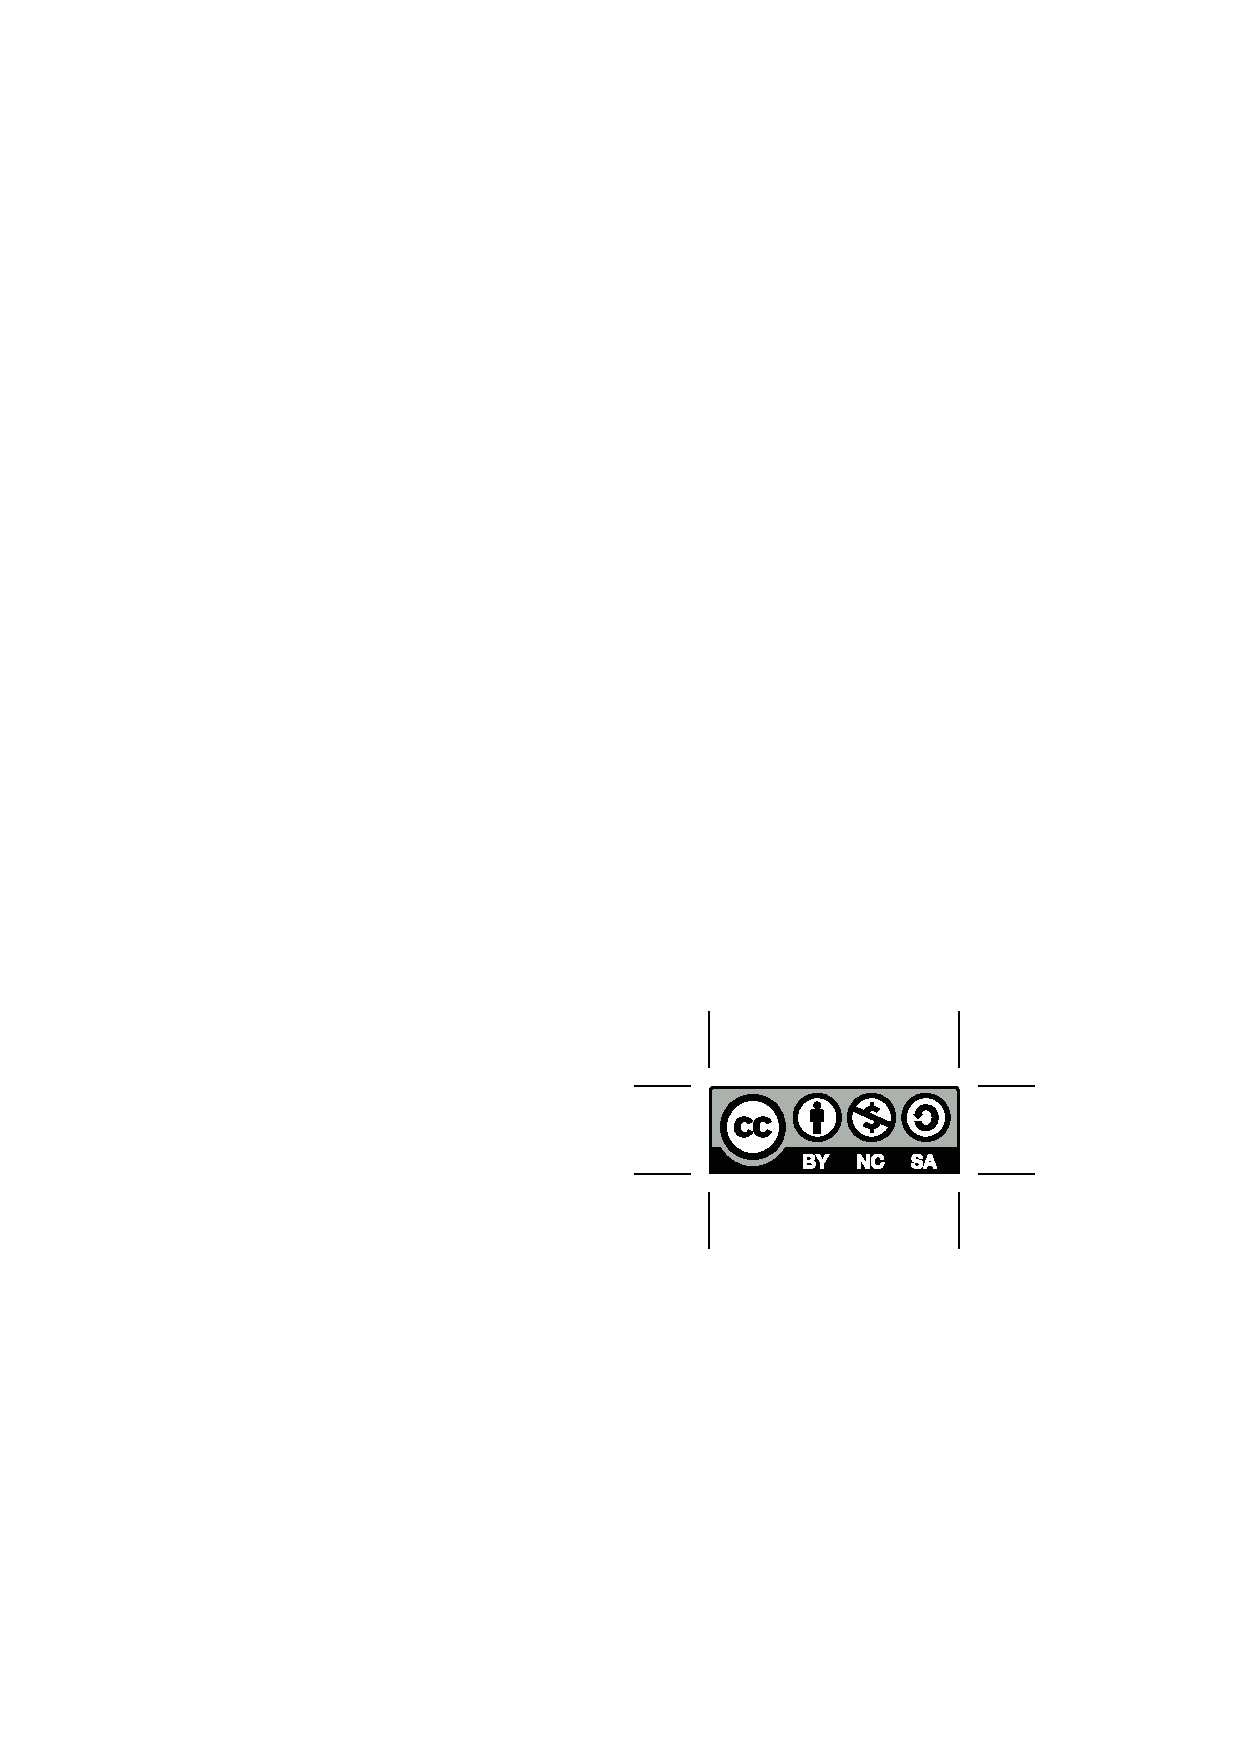
\includegraphics[width=1.38in]{figures/license}
\quad

\includegraphics[width=1.38in]{figures/license2}
%\end{floatingfigure}

\bigskip

\noindent
\textbf{License:}
\\
This work is dual licensed under
the Creative Commons
Attribution-Non\-commercial-Share Alike 4.0 International License and
the Creative Commons
Attribution-Share Alike 4.0 International License.
To view a
copy of these licenses, visit
\url{https://creativecommons.org/licenses/by-nc-sa/4.0/}
or
\url{https://creativecommons.org/licenses/by-sa/4.0/}
or send a letter to
Creative Commons
PO Box 1866, Mountain View, CA 94042, USA\@.
%Creative Commons, 171 Second Street, Suite 300, San Francisco, California,
%94105, USA.

\bigskip

\noindent
You can use, print, duplicate, share this book as much as you want.  You can
base your own notes on it and reuse parts if you keep the license the
same.  You can assume the license is either the CC-BY-NC-SA or CC-BY-SA\@,
whichever is compatible with what you wish to do, your derivative works must
use at least one of the licenses.

\bigskip

\noindent
\textbf{Acknowledgments:}
\\
I would like to thank Debraj Chakrabarti, Anirban Dawn, Alekzander Malcom,
John Treuer, Jianou Zhang, Liz Vivas, Trevor Fancher,
and students in my classes for pointing out typos/errors
and helpful suggestions. 

\bigskip

\noindent
During the writing of this book, 
the author was in part supported by NSF grant DMS-1362337.

\bigskip

\noindent
\textbf{More information:}
\\
See \url{https://www.jirka.org/scv/} for more information
(including contact information).

\medskip

\noindent
The \LaTeX\ source for the book is available
for possible modification and customization
at github: \url{https://github.com/jirilebl/scv}


% For large print do this
%\large

\microtypesetup{protrusion=false}
\tableofcontents
\microtypesetup{protrusion=true}

%\addtocontents{toc}{\protect\vspace{-2\baselineskip}}
\addtocontents{toc}{\protect\vspace{-\baselineskip}}
%\addtocontents{toc}{\protect\enlargethispage{\baselineskip}}

%%%%%%%%%%%%%%%%%%%%%%%%%%%%%%%%%%%%%%%%%%%%%%%%%%%%%%%%%%%%%%%%%%%%%%%%%%%%%%
%%%%%%%%%%%%%%%%%%%%%%%%%%%%%%%%%%%%%%%%%%%%%%%%%%%%%%%%%%%%%%%%%%%%%%%%%%%%%%
%%%%%%%%%%%%%%%%%%%%%%%%%%%%%%%%%%%%%%%%%%%%%%%%%%%%%%%%%%%%%%%%%%%%%%%%%%%%%%

\chapter*{Introduction} \label{ch:intro}
\addcontentsline{toc}{chapter}{Introduction}
\markboth{INTRODUCTION}{INTRODUCTION}

%%%%%%%%%%%%%%%%%%%%%%%%%%%%%%%%%%%%%%%%%%%%%%%%%%%%%%%%%%%%%%%%%%%%%%%%%%%%%%

This book is a polished version of my course notes for Math 6283, Several
Complex Variables, given in
Spring 2014, Spring 2016, and then Spring 2019 semesters
at Oklahoma State University.
It is meant for a semester-long course.
There are quite a few
exercises sprinkled throughout the text, and I am assuming that a reader is
at least attempting all of them.  Many are required later in the
text.  The reader should attempt exercises in sequence as earlier exercises
can help or even be required to solve later exercises.

The prerequisites are a decent knowledge of vector calculus, basic
real-analysis, and a working knowledge of complex analysis in one variable.
It is accessible to beginning graduate students after a complex
analysis course, and the background actually required is quite minimal.
Towards the end of the course (mainly \chapterref{ch:integralkernels}),
differential forms will be useful, and
in the final chapter, \chapterref{ch:analyticvarieties},
we will use some basic ring theory from algebra.

This book is not meant as an exhaustive reference.  It is simply a whirlwind
tour of several complex variables.  See the end of the book
for a \hyperref[ch:furtherreading]{list of books} useful for
reference and further reading.  There are also two appendices for
a list of useful one-variable results and overview of differential forms,
see \appendixref{ap:onevarresults} and
\appendixref{ap:diffforms}.

%%%%%%%%%%%%%%%%%%%%%%%%%%%%%%%%%%%%%%%%%%%%%%%%%%%%%%%%%%%%%%%%%%%%%%%%%%%%%%

\section{Motivation, single variable, and Cauchy's formula} \label{sec:motivation}


Let us start with some standard notation.
We use \glsadd{not:C}$\C$ for the complex numbers, \glsadd{not:R}$\R$
for real numbers,
\glsadd{not:Z}$\Z$ for integers,
\glsadd{not:N}$\N = \{ 1,2,3,\ldots \}$ for natural
numbers,
\glsadd{not:i}$i = \sqrt{-1}$, etc.  Throughout this book, we will use
the standard terminology of \emph{\myindex{domain}} to mean connected open
set.

As complex analysis deals with the complex numbers, perhaps we should start
with $\sqrt{-1}$.  We start with the real numbers, $\R$, and wish to add
$\sqrt{-1}$ into our field.  We call this square root $i$, and we write the
complex numbers, $\C$, by
identifying 
$\C$ with $\R^2$ using
\begin{equation*}
z = x+iy,
\end{equation*}
where $z \in \C$, and $(x,y) \in \R^2$.  
A subtle philosophical issue is that there are two square roots of $-1$.
There are 
two chickens running around in our yard, and because we like to
know which is which, we catch one and write ``$i$'' on it.  If we happened
to have caught the other chicken, we would have gotten an exactly equivalent
theory, which we could not tell apart from the original.

Given a complex number $z$, its ``opposite'' is 
the \emph{\myindex{complex conjugate}} of $z$ and is defined as
\glsadd{not:conj}%
\begin{equation*}
\bar{z} \overset{\text{def}}{=} x-iy.
\end{equation*}
The size of $z$ is measured by the so-called \emph{\myindex{modulus}},
which is really just the \emph{\myindex{Euclidean distance}}:
\glsadd{not:mod}%
\begin{equation*}
\abs{z} \overset{\text{def}}{=} \sqrt{z \bar{z}} = \sqrt{x^2+y^2} .
\end{equation*}

If $z = x+iy \in \C$ for $x,y \in \R$, then $x$ is called the
\emph{\myindex{real part}} and $y$ is called the
\emph{\myindex{imaginary part}} and we write
\glsadd{not:real}%
\glsadd{not:imag}%
\begin{equation*}
\Re z = 
\Re (x+iy) =
\frac{z+\bar{z}}{2}
= x, \qquad 
\Im z = 
\Im (x+iy) =
\frac{z-\bar{z}}{2i}
=
y .
\end{equation*}


A function $f \colon U \subset \R^n \to \C$ for an open set $U$
is said to be continuously differentiable, or $C^1$ if the first (real)
partial derivatives exist and are continuous.
\glsadd{not:Ck}%
Similarly, it is $C^k$ or \emph{$C^k$-smooth}
\index{Ck-smooth function@$C^k$-smooth function}
if the first $k$ partial derivatives all exist and are differentiable.
\glsadd{not:Cinfty}%
Finally, a function is said to be $C^\infty$ or simply
\emph{smooth}\index{smooth function}\footnote{%
While $C^\infty$ is the common definition of \emph{smooth}, not everyone
always means
the same thing by the word \emph{smooth}.  I have seen it mean
differentiable, $C^1$, piecewise-$C^1$, $C^\infty$, holomorphic, \ldots}
if it is \emph{\myindex{infinitely differentiable}},
or in other words, if it is $C^k$ for all $k \in \N$.

\medskip

Complex analysis is the study of holomorphic (or complex-analytic)
functions.
There is an awful lot one can do with polynomials, but sometimes they are
just not enough.  For example, there is no nonzero polynomial function that solves
the simplest of differential equations, $f' = f$.  We need the exponential
function, which is holomorphic.  
Holomorphic functions are a generalization of polynomials,
and to get there one leaves the land of algebra to arrive in the realm of
analysis.

Let us start with polynomials.  In one variable, a polynomial in $z$ is
an expression of the form
\begin{equation*}
P(z) = \sum_{j=0}^d c_j \, z^j ,
\end{equation*}
where $c_j \in \C$ and $c_d \not= 0$.  The number $d$ is called the
\emph{degree}\index{degree of a polynomial}
of the
polynomial $P$.  We can plug in some number $z$ and simply compute
$P(z)$, so we have a function $P \colon \C \to \C$.

We try to write
\begin{equation*}
f(z) = \sum_{j=0}^\infty c_j \, z^j
\end{equation*}
and all is very fine until we wish to know what $f(z)$ is for some number
$z \in \C$.
We usually mean 
\begin{equation*}
\sum_{j=0}^\infty c_j \, z^j
=
\lim_{d\to\infty}
\sum_{j=0}^d c_j \, z^j .
\end{equation*}
As long as the limit exists, we have a function.  You know all
this; it is your one-variable complex analysis.  We usually
start with the functions and prove that we can expand into series.

Let $U \subset \C$ be open.  A function $f \colon U \to \C$
is \emph{\myindex{holomorphic}}
(or \emph{\myindex{complex-analytic}}) if it is
\emph{\myindex{complex-differentiable}} at every point,
that is, if
\begin{equation*}
f'(z)
%=
%\lim_{w \in \C \to z} \frac{f(w)-f(z_0)}{w-z} 
=
\lim_{\xi \in \C \to 0} \frac{f(z+\xi)-f(z)}{\xi} 
\qquad \text{exists for all $z \in U$.}
\end{equation*}
Importantly, the limit is taken with respect to
complex %$w$ or
$\xi$.
Another vantage point is to start with a continuously 
differentiable\footnote{Holomorphic functions end up being infinitely
differentiable anyway, so this hypothesis is not overly restrictive.} $f$,
and say that $f = u + i\, v$ is holomorphic if it satisfies
the \emph{\myindex{Cauchy--Riemann equations}}:
\begin{equation*}
\frac{\partial u}{\partial x} = 
\frac{\partial v}{\partial y} ,
\qquad
\frac{\partial u}{\partial y} = 
-
\frac{\partial v}{\partial x} .
\end{equation*}
The so-called \emph{\myindex{Wirtinger operators}},
\begin{equation*}
\frac{\partial}{\partial z}
\overset{\text{def}}{=}
\frac{1}{2}
\left(
\frac{\partial}{\partial x} - i
\frac{\partial}{\partial y}
\right),
~ ~ ~ ~ ~
\frac{\partial}{\partial \bar{z}}
\overset{\text{def}}{=}
\frac{1}{2}
\left(
\frac{\partial}{\partial x} + i
\frac{\partial}{\partial y}
\right)
,
\end{equation*}
provide an easier way to understand the
Cauchy--Riemann equations.
These operators are determined by insisting
\glsadd{not:wirt}%
\begin{equation*}
\frac{\partial}{\partial z} z = 1, \quad
\frac{\partial}{\partial z} \bar{z} = 0, \quad
\frac{\partial}{\partial \bar{z}} z = 0, \quad
\frac{\partial}{\partial \bar{z}} \bar{z} = 1.
\end{equation*}

The function $f$ is holomorphic if and only if
\begin{equation*}
\frac{\partial f}{\partial \bar{z}} = 0 .
\end{equation*}
That seems a far nicer statement of the Cauchy--Riemann equations, and it is
now just one complex equation.  It says
a function is holomorphic if and only if it depends on $z$ but not on
$\bar{z}$ (perhaps that might not make a whole lot of sense at first
glance).
Let us check:
\begin{equation*}
\frac{\partial f}{\partial \bar{z}} 
=
\frac{1}{2}
\left(
\frac{\partial f}{\partial x} + i
\frac{\partial f}{\partial y}
\right)
=
%\frac{1}{2}
%\left(
%\frac{\partial }{\partial x} (u + iv) + i
%\frac{\partial }{\partial y} (u + iv)
%\right)
%=
\frac{1}{2}
\left(
\frac{\partial u}{\partial x} 
+ i \frac{\partial v}{\partial x} 
+ i \frac{\partial u}{\partial y}
- \frac{\partial v}{\partial y}
\right) 
=
\frac{1}{2}
\left(
\frac{\partial u}{\partial x} 
- \frac{\partial v}{\partial y}
\right)
+
\frac{i}{2}
\left(
\frac{\partial v}{\partial x} 
+ \frac{\partial u}{\partial y}
\right) .
\end{equation*}
This expression is zero if and only if the real parts and the imaginary
parts are zero.  In other words %if and only if
\begin{equation*}
\frac{\partial u}{\partial x} 
- \frac{\partial v}{\partial y}
= 0,
\qquad
\text{and}
\qquad
\frac{\partial v}{\partial x} 
+ \frac{\partial u}{\partial y} = 0
.
\end{equation*}
That is, the Cauchy--Riemann equations are satisfied.

%Another common way to define a holomorphic function is to say that
%the complex derivative at each point exists.  If $f'$ exists
%at every point, it equals the derivative in $z$.
If $f$ is holomorphic, the derivative in $z$ is the standard complex derivative you know and love:
\begin{equation*}
\frac{\partial f}{\partial z} (z_0)
=
f'(z_0)
=
\lim_{\xi \to 0} \frac{f(z_0+\xi)-f(z_0)}{\xi} .
\end{equation*}
That's because 
\begin{equation*}
\begin{split}
\frac{\partial f}{\partial z} 
=
\frac{1}{2}
\left(
\frac{\partial u}{\partial x} 
+ \frac{\partial v}{\partial y}
\right)
+
\frac{i}{2}
\left( \frac{\partial v}{\partial x} - \frac{\partial u}{\partial y}
\right) 
& =
\frac{\partial u}{\partial x} 
+ i \frac{\partial v}{\partial x}
 =
\frac{\partial f}{\partial x}
\\
& =
\frac{1}{i} \left(
\frac{\partial u}{\partial y}
+ i
\frac{\partial v}{\partial y} 
\right)
 =
\frac{\partial f}{\partial (iy)}
.
\end{split}
\end{equation*}

A function on $\C$ is really a function defined on
$\R^2$ as identified above and hence it is a function of $x$ and $y$.
Writing
$x = \frac{z+\bar{z}}{2}$ and
$y = \frac{z-\bar{z}}{2i}$, we think of it as a function of two
complex variables $z$ and $\bar{z}$.  Pretend for a moment as if $\bar{z}$ did not
depend on $z$.
The Wirtinger operators
work as if $z$ and $\bar{z}$ really were independent variables.  For example:
\begin{equation*}
\frac{\partial}{\partial z}
\left[ z^2 \bar{z}^3 + z^{10} \right]
=
2z \bar{z}^3 + 10 z^{9}
\qquad
\text{and}
\qquad
\frac{\partial}{\partial \bar{z}}
\left[ z^2 \bar{z}^3 + z^{10} \right]
=
z^2 ( 3 \bar{z}^2 ) + 0 .
\end{equation*}
So a holomorphic function is a function not depending on $\bar{z}$.

One of the most important theorems in one variable is
the \emph{\myindex{Cauchy integral formula}}\index{Cauchy formula}.

\begin{thm}[Cauchy integral formula]
Let $U \subset \C$ be a bounded domain where the boundary $\partial U$
is a piecewise smooth
simple closed path (a Jordan curve).  Let $f \colon \overline{U} \to \C$ be a continuous function,
holomorphic in $U$.
Orient $\partial U$ positively (going around counter-clockwise).
Then
\begin{equation*}
f(z) =
\frac{1}{2\pi i}
\int_{\partial U}
\frac{f(\zeta)}{\zeta-z}
\,
d \zeta 
\qquad \text{for all $z \in U$.}
\end{equation*}
\end{thm}

%The path integral for a smooth path $\gamma \colon [a,b] \to \C$ is defined as
%\begin{equation*}
%\int_\gamma f(z) \, dz
%=
%\int_a^b f\bigl(\gamma(t)\bigr) \gamma'(t) \, dt .
%\end{equation*}

The Cauchy formula is the essential ingredient we need from 
one complex variable.  It follows, for example,
from Green's theorem (Stokes' theorem in two
dimensions).  You can look forward to
\thmref{thm:generalizedcauchy} for a proof of a more general formula,
the Cauchy--Pompeiu integral formula.

As a differential form, \glsadd{not:dz}$dz = dx + i \, dy$.  If you are uneasy
about differential forms, you probably defined the path integral above
directly using
the Riemann--Stieltjes integral in your one-complex-variable class.
Let us write down the formula in terms of the standard Riemann integral
in a special case.  Take the \emph{\myindex{unit disc}}
\glsadd{not:D}%
\begin{equation*}
\D
\overset{\text{def}}{=}
\bigl\{ z \in \C : \sabs{z} < 1 \bigr\} .
\end{equation*}
The boundary is the unit circle
$\partial \D = \bigl\{ z \in \C : \sabs{z} = 1 \bigr\}$ oriented positively,
that is, counter-clockwise.   Parametrize $\partial \D$
by $e^{it}$, where $t$ goes from 0 to $2\pi$.  If $\zeta = e^{it}$,
then $d\zeta = ie^{it}dt$, and
\begin{equation*}
f(z) =
\frac{1}{2\pi i}
\int_{\partial \D}
\frac{f(\zeta)}{\zeta-z}
\,
d \zeta 
=
\frac{1}{2\pi}
\int_0^{2\pi}
\frac{f(e^{it}) e^{it} }{e^{it}-z}
\,
dt .
\end{equation*}
If you are not completely comfortable
with
path %or surface
integrals, try to think about how you would parametrize the path, and
write the integral as an integral any calculus student would recognize.

I venture a guess that 90\% of what you learned in a one-variable complex analysis
course (depending on who taught it)
is more or less a straightforward consequence of the Cauchy
integral formula.
An important theorem from one variable that follows from
the Cauchy formula is the
\emph{\myindex{maximum modulus principle}} (or just
the \emph{\myindex{maximum principle})},
which has several versions.  Let us give the simplest one.

\begin{thm}[Maximum modulus principle]
Suppose $U \subset \C$ is a domain and $f \colon U \to \C$
is holomorphic.
If for some $z_0 \in U$
\begin{equation*}
\sup_{z \in U} \, \sabs{f(z)} = \sabs{f(z_0)} ,
\end{equation*}
\glsadd{not:identeq}%
then $f$ is constant, that is, $f \equiv f(z_0)$.
\end{thm}

That is, if the supremum is attained in the interior of the domain,
then the function must be constant.  Another way to state the maximum
principle is to say: if $f$ extends continuously to the boundary of a
domain, then the supremum of $\sabs{f(z)}$ is attained on the boundary.
In
one variable you learned that the maximum principle is really a
property of harmonic functions.

\begin{thm}[Maximum principle]
Let $U \subset \C$ be a domain and $h \colon U \to \R$
harmonic, that is,
\glsadd{not:laplacian}%
\begin{equation*}
\nabla^2 h = \frac{\partial^2 h}{\partial x^2} + \frac{\partial^2 h}{\partial
y^2} = 0 .
\end{equation*}
If for some $z_0 \in U$
\begin{equation*}
\sup_{z \in U} \, h(z) = h(z_0)
\qquad \text{or} \qquad
\inf_{z \in U} \, h(z) = h(z_0) ,
\end{equation*}
then $h$ is constant, that is, $h \equiv h(z_0)$.
\end{thm}

In one variable, if $f = u+iv$ is holomorphic for real valued $u$ and $v$,
then $u$ and $v$ are harmonic.  Locally, any harmonic function is
the real (or imaginary) part of a holomorphic function, so in
one complex variable, studying 
harmonic functions is almost equivalent to studying holomorphic
functions.  Things are decidedly different
in two or more variables.

\medskip

Holomorphic functions admit a power series representation in $z$
at each point $a$:
\begin{equation*}
f(z) = \sum_{j=0}^\infty c_j {(z-a)}^j .
\end{equation*}
There is no $\bar{z}$ necessary there
since $\frac{\partial f}{\partial \bar{z}} = 0$.

Let us see the proof using the Cauchy integral formula as we will
require this computation in several variables as well.
Given $a \in \C$ and $\rho > 0$, define the disc of radius $\rho$ around $a$
\glsadd{not:disc}%
\begin{equation*}
\Delta_\rho(a)
\overset{\text{def}}{=}
\bigl\{ z \in \C : \sabs{z-a} < \rho \bigr\} .
\end{equation*}
Suppose $U \subset \C$ is a domain, $f \colon U \to \C$ is holomorphic,
$a \in U$, and $\overline{\Delta_\rho(a)} \subset U$ (that is, the closure
of the disc is in $U$, and so its boundary $\partial \Delta_\rho(a)$ is also in $U$).

For $z \in \Delta_\rho(a)$ and $\zeta \in \partial \Delta_\rho(a)$, 
\begin{equation*}
\abs{\frac{z-a}{\zeta-a}} =
\frac{\sabs{z-a}}{\rho} < 1 .
\end{equation*}
In fact, if $\sabs{z-a} \leq \rho' < \rho$, then
$\abs{\frac{z-a}{\zeta-a}} \leq \frac{\rho'}{\rho} < 1$.  Therefore,
the geometric series
\begin{equation*}
\sum_{j=0}^\infty
{\left(\frac{z-a}{\zeta-a}\right)}^j
=
\frac{1}{1-
\frac{z-a}{\zeta-a}}
=
\frac{\zeta-a}{\zeta-z}
\end{equation*}
converges uniformly absolutely for $(z,\zeta) \in \overline{\Delta_{\rho'}(a)}
\times \partial \Delta_\rho(a)$ (that is, $\sum_j {\bigl\lvert
\frac{z-a}{\zeta-a} \bigr\rvert}^j$
converges uniformly).
%In particular, the
%series converges uniformly absolutely in $z$ on compact subsets of $\Delta_{\rho}(a)$. 

Let $\gamma$
be the path going around 
$\partial \Delta_\rho(a)$ once in the positive direction.  Compute
\begin{equation*}
\begin{split}
f(z)
& =
\frac{1}{2\pi i}
\int_{\gamma}
\frac{f(\zeta)}{\zeta-z}
\,
d \zeta 
\\
& =
\frac{1}{2\pi i}
\int_{\gamma}
\frac{f(\zeta)}{\zeta-a}
\frac{\zeta-a}{\zeta-z}
\,
d \zeta 
\\
& =
\frac{1}{2\pi i}
\int_{\gamma}
\frac{f(\zeta)}{\zeta-a}
\sum_{j=0}^\infty
{\left(\frac{z-a}{\zeta-a}\right)}^j
\,
d \zeta 
\\
& =
\sum_{j=0}^\infty
\left(
\frac{1}{2\pi i}
\int_{\gamma}
\frac{f(\zeta)}{{(\zeta-a)}^{j+1}}
\,
d \zeta 
\right)
{(z-a)}^j .
\end{split}
\end{equation*}
In the last equality, we are allowed to 
interchange the limit on the sum with the integral either
by Fubini's theorem or by uniform convergence:
$z$ is fixed and if $M$ is the supremum of $\abs{\frac{f(\zeta)}{\zeta-a}} =
\frac{\sabs{f(\zeta)}}{\rho}$ on $\partial \Delta_\rho(a)$,
then
\begin{equation*}
\abs{
\frac{f(\zeta)}{\zeta-a}
{\left(\frac{z-a}{\zeta-a}\right)}^j
}
\leq
M 
{\left(\frac{\abs{z-a}}{\rho}\right)}^j,
\qquad \text{and} \qquad
\frac{\abs{z-a}}{\rho} < 1 .
\end{equation*}

The key point is writing the \emph{\myindex{Cauchy kernel}}
$\frac{1}{\zeta-z}$ as
\begin{equation*}
\frac{1}{\zeta-z}
=
\frac{1}{\zeta-a}
\frac{\zeta-a}{\zeta-z} ,
\end{equation*}
and then using the geometric series.

Not only have we proved that $f$ has a power series, but we computed
that the radius of convergence is at least $R$, where $R$ is the maximum $R$
such that $\Delta_R(a) \subset U$.  We also obtained a formula for the
coefficients
\begin{equation*}
c_j = 
\frac{1}{2\pi i}
\int_{\gamma}
\frac{f(\zeta)}{{(\zeta-a)}^{j+1}}
\,
d \zeta  .
\end{equation*}

For a set $K$ denote the \emph{\myindex{supremum norm}}:
\glsadd{not:supnorm}%
\begin{equation*}
\snorm{f}_K
\overset{\text{def}}{=}
\sup_{z \in K} \sabs{f(z)} .
\end{equation*}
By a brute force estimation, we obtain the very useful
\emph{\myindex{Cauchy estimates}}:
\begin{equation*}
\sabs{c_j} = 
\abs{
\frac{1}{2\pi i}
\int_{\gamma}
\frac{f(\zeta)}{{(\zeta-a)}^{j+1}}
\,
d \zeta 
}
\leq
\frac{1}{2\pi}
\int_{\gamma}
\frac{\snorm{f}_{\gamma}}{\rho^{j+1}}
\,
\sabs{d \zeta} 
=
\frac{\snorm{f}_{\gamma}}{\rho^{j}} .
\end{equation*}

We differentiate Cauchy's formula $j$ times (using the Wirtinger
$\frac{\partial}{\partial z}$ operator),
\begin{equation*}
f^{(j)}(z)
=
\frac{\partial^j f}{\partial z^j} (z)
=
\frac{1}{2\pi i}
\int_{\gamma}
\frac{j! f(\zeta)}{{(\zeta-z)}^{j+1}}
\,
d \zeta  ,
\end{equation*}
and therefore
\begin{equation*}
j! \, c_j =
f^{(j)}(a)
=
\frac{\partial^j f}{\partial z^j}(a) .
\end{equation*}
Consequently,
This estimate says that we can control derivatives of $f$
by the size of the function.  This is one of the key properties of
holomorphic functions, and the reason why the proper topology for
the set of holomorphic functions is the same as the topology for continuous functions.
\begin{equation*}
\babs{f^{(j)}(a)}
=
\abs{\frac{\partial^j f}{\partial z^j}(a)}
\leq
\frac{j! \snorm{f}_{\gamma}}{\rho^{j}} .
\end{equation*}
This estimate says that we can control derivatives of $f$ by the size of the
function.  This is one of the key properties of holomorphic functions, and
the reason why the proper topology for the set of holomorphic functions is
the same as the topology for continuous functions.  Consequently,
obstructions to solving problems in complex analysis are often topological
in character.

For further review of one-variable results useful in this book,
see \appendixref{ap:onevarresults}.

%%%%%%%%%%%%%%%%%%%%%%%%%%%%%%%%%%%%%%%%%%%%%%%%%%%%%%%%%%%%%%%%%%%%%%%%%%%%%%
%%%%%%%%%%%%%%%%%%%%%%%%%%%%%%%%%%%%%%%%%%%%%%%%%%%%%%%%%%%%%%%%%%%%%%%%%%%%%%
%%%%%%%%%%%%%%%%%%%%%%%%%%%%%%%%%%%%%%%%%%%%%%%%%%%%%%%%%%%%%%%%%%%%%%%%%%%%%%

\chapter{Holomorphic functions in several variables} \label{ch:holfunc}

%%%%%%%%%%%%%%%%%%%%%%%%%%%%%%%%%%%%%%%%%%%%%%%%%%%%%%%%%%%%%%%%%%%%%%%%%%%%%%

\section{Onto several variables} \label{sec:ontosevvar}

Let $\C^n = \overbrace{\C \times \C \times \cdots \times \C}^{\text{$n$
times}}$ denote the $n$-dimensional
\emph{\myindex{complex Euclidean space}}\index{Euclidean space}.  Denote
by $z = (z_1,z_2,\ldots,z_n)$ the coordinates of $\C^n$.
Let $x =
(x_1,x_2,\ldots,x_n)$ and $y = (y_1,y_2,\ldots,y_n)$ denote coordinates in
$\R^n$.
We 
identify $\C^n$ with
$\R^{2n}$ by letting
$z = x+iy$, that is, $z_j = x_j + i y_j$ for every $j$.
As in one complex variable, we write $\bar{z} = x-iy$.
We call $z$ the \emph{\myindex{holomorphic coordinates}}
and $\bar{z}$ the \emph{\myindex{antiholomorphic coordinates}}.

\begin{defn}
For $\rho = (\rho_1,\rho_2,\ldots,\rho_n)$ where $\rho_j > 0$ and $a \in \C^n$,
define
a \emph{\myindex{polydisc}}
\glsadd{not:disc}%
\begin{equation*}
\Delta_\rho(a)  \overset{\text{def}}{=}
\bigl\{ z \in \C^n : \sabs{z_j - a_j} < \rho_j ~\text{for $j=1,2,\ldots,n$} \bigr\} .
\end{equation*}
We call $a$ the
\emph{center}\index{center of a polydisc}
and $\rho$ the
\emph{polyradius}\index{polyradius of a polydisc}
or simply the
\emph{radius}\index{radius of a polydisc}
of the polydisc $\Delta_\rho(a)$.
If $\rho > 0$ is a number, then
\begin{equation*}
\Delta_\rho(a)  \overset{\text{def}}{=}
\bigl\{ z \in \C^n : \sabs{z_j - a_j} < \rho ~\text{for $j=1,2,\ldots,n$} \bigr\} .
\end{equation*}
In two variables, a polydisc is sometimes called a \emph{\myindex{bidisc}}.

As there is the unit disc $\D$ in one variable, so is there
the \emph{\myindex{unit polydisc}} in several variables:
\begin{equation*}
\D^n = \D \times \D \times \cdots \times \D = \Delta_1(0) = 
\bigl\{ z \in \C^n : \sabs{z_j} < 1 ~\text{for $j=1,2,\ldots,n$} \bigr\} .
\end{equation*}
\end{defn}

In more than one complex dimension, it is difficult to draw exact pictures
for lack of real dimensions on our paper.
We visualize the unit polydisc in two variables
by drawing the following
picture by plotting just against the modulus of the variables:
\begin{myfig}
\subimport*{figures/}{polydisc.pdf_t}
\end{myfig}

Recall the
\emph{\myindex{Euclidean inner product}} on $\C^n$:
\glsadd{not:hermprod}%
\begin{equation*}
\linnprod{z}{w} \overset{\text{def}}{=} %z \cdot \bar{w}
z_1 \bar{w}_1 +
z_2 \bar{w}_2 + \cdots +
z_n \bar{w}_n .
\end{equation*}
The inner product gives us the standard
\emph{\myindex{Euclidean norm}} on $\C^n$:
\glsadd{not:eucnorm}%
\begin{equation*}
\snorm{z}  \overset{\text{def}}{=} \sqrt{\linnprod{z}{z}}
=
\sqrt{\sabs{z_1}^2 +
\sabs{z_2}^2 + \cdots +
\sabs{z_n}^2} .
\end{equation*}
This norm agrees with the standard Euclidean norm on $\R^{2n}$.
Define \emph{balls}\index{ball} as in $\R^{2n}$:
\glsadd{not:ball}%
\begin{equation*}
B_\rho(a)  \overset{\text{def}}{=}
\bigl\{ z \in \C^n : \snorm{z - a} < \rho \bigr\} ,
\end{equation*}
And define the \emph{\myindex{unit ball}} as
\glsadd{not:unitball}%
\begin{equation*}
\bB_n \overset{\text{def}}{=} B_1(0) =
\bigl\{ z \in \C^n : \snorm{z} < 1 \bigr\} .
\end{equation*}

A ball centered at the origin
can also be pictured by plotting against the modulus of the
variables since the inequality defining the ball only
depends on the moduli of the variables.
Not every domain can be drawn like this, but those that can
are called \emph{\myindex{Reinhardt domain}}, more on this later.
Here is a picture of $\bB_2$:
\begin{myfig}
\subimport*{figures/}{ball.pdf_t}
\end{myfig}

\begin{defn}
Let $U \subset
\C^n$ be an open set.  A
function
$f \colon U \to \C$ is \emph{\myindex{holomorphic}} if
it is \emph{locally bounded}%
\index{locally bounded function}\footnote{For
every $p \in U$, there is a neighborhood $N$ of $p$
such that $f|_N$ is bounded.  It is a deep result of Hartogs that we might
in fact just drop ``locally bounded'' from the definition and obtain the same
set of functions.}
%A deep result of Hartogs, which we skip, says that
%we do not need to assume $f$ to be locally bounded.}
and holomorphic in each variable separately.
In other words, $f$ is holomorphic if it is locally bounded
and complex-differentiable in each variable separately:
\begin{equation*}
\lim_{\xi \in \C \to 0} \frac{f(z_1,\ldots,z_k+\xi,\ldots,z_n) - f(z)}{\xi}
\qquad \text{exists for all $z \in U$ and all $k=1,2,\ldots,n$}.
\end{equation*}
In this book, however, the words ``differentiable'' and ``derivative''
(without the ``complex-'') refer
to plain vanilla real differentiability.
\end{defn}

As in one variable, we define the \emph{\myindex{Wirtinger operators}}
\glsadd{not:wirt}%
\begin{equation*}
\frac{\partial}{\partial z_j}  \overset{\text{def}}{=}
\frac{1}{2} \left(
\frac{\partial}{\partial x_j} - i \frac{\partial}{\partial y_j}
\right) ,
\qquad
\frac{\partial}{\partial \bar{z}_j}  \overset{\text{def}}{=}
\frac{1}{2} \left(
\frac{\partial}{\partial x_j} + i \frac{\partial}{\partial y_j}
\right) .
\end{equation*}
An alternative definition is to say that a continuously
differentiable function $f \colon U \to \C$ is
\emph{holomorphic} if
it satisfies the
\emph{\myindex{Cauchy--Riemann equations}}
\begin{equation*}
\frac{\partial f}{\partial \bar{z}_j}  = 0 \qquad \text{for $j=1,2,\ldots,n$}.
\end{equation*}
As in one variable, if you defined partial derivatives
of holomorphic functions
as the limits of the definition above,
then you would get the Wirtinger $\frac{\partial}{\partial z_k}$
for holomorphic functions.  That is, if $f$ is holomorphic, then
\begin{equation*}
\frac{\partial f}{\partial z_k}(z)
=
\lim_{\xi \in \C \to 0} \frac{f(z_1,\ldots,z_k+\xi,\ldots,z_n) - f(z)}{\xi}
.
\end{equation*}

Due to the following proposition, the alternative definition using the
Cauchy--Riemann equations is just as good as the definition we gave.

\begin{prop}
Let $U \subset \C^n$ be an open set and
suppose $f \colon U \to \C$ is holomorphic.  Then $f$ is infinitely
differentiable.
\end{prop}

\begin{proof}
Suppose $\Delta = \Delta_{\rho}(a) = \Delta_1 \times \cdots \times \Delta_n$
is a polydisc centered at $a$, where each $\Delta_j$ is a disc
and suppose $\overline{\Delta} \subset U$, that is, $f$ is holomorphic
on a neighborhood of the closure of $\Delta$.
Let $z$ be in $\Delta$.
Orient $\partial \Delta_1$ positively and
apply the Cauchy formula (after all $f$ is holomorphic in $z_1$):
\begin{equation*}
f(z) =
\frac{1}{2\pi i}
\int_{\partial \Delta_1}
\frac{f(\zeta_1,z_2,\ldots,z_n)}{\zeta_1-z_1}
\,
d \zeta_1 .
\end{equation*}
Apply it again on the second variable, again orienting
$\partial \Delta_2$ positively:
\begin{equation*}
f(z) =
\frac{1}{{(2\pi i)}^2}
\int_{\partial \Delta_1}
\int_{\partial \Delta_2}
\frac{f(\zeta_1,\zeta_2,z_3,\ldots,z_n)}{(\zeta_1-z_1)(\zeta_2-z_2)}
\,
d \zeta_2
\,
d \zeta_1 .
\end{equation*}

Applying the formula $n$ times we obtain
\begin{equation} \label{iteratedcauchy:eq}
f(z) =
\frac{1}{{(2\pi i)}^n}
\int_{\partial \Delta_1}
\int_{\partial \Delta_2}
\cdots
\int_{\partial \Delta_n}
\frac{f(\zeta_1,\zeta_2,\ldots,\zeta_n)}{(\zeta_1-z_1)(\zeta_2-z_2)\cdots(\zeta_n-z_n)}
\,
d \zeta_n
\cdots
d \zeta_2
\,
d \zeta_1 .
\end{equation}
As $f$ is bounded on the compact set
$\partial \Delta_1 \times \cdots \times \partial \Delta_n$,
we find that $f$ is continuous in $\Delta$.
We may differentiate underneath the
integral, because $f$ is bounded on 
$\partial \Delta_1 \times \cdots \times \partial \Delta_n$
and so are the derivatives of the integrand
with respect to $x_j$ and $y_j$, where $z_j=x_j+i y_j$, as long as
$z$ is a positive distance away from
$\partial \Delta_1 \times \cdots \times \partial \Delta_n$.
We may differentiate as many times as we wish.
%We are really differentiating only in the real and imaginary
%parts of the $z_j$ variables, and the integrand is
%infinitely differentiable in those variables.
\end{proof}

%In the definition of holomorphicity,
%we may have assumed $f$ is smooth and satisfies
%the Cauchy--Riemann equations.  However, the way we stated the
%definition makes it easier to apply.

Above in \eqref{iteratedcauchy:eq}, we really derived the Cauchy integral formula in several variables.  To
write the formula more concisely we apply the Fubini's theorem to write it as
a single integral.  We will write it down using differential forms.  If you
are unfamiliar with differential forms, think of the integral
as the iterated integral above, and you can read the next few paragraphs
a little lightly.
It is enough to understand real differential forms; we simply allow
complex coefficients.
For a good introduction to differential forms
see Rudin~\cite{Rudin:principles}.

Recall that given coordinates $x = (x_1,\ldots,x_n)$, a one-form $d x_j$ is a linear functional on tangent vectors
such that when $d x_j \bigl( \frac{\partial}{\partial x_j} \bigr) = 1$ and
$d x_j \bigl( \frac{\partial}{\partial x_k} \bigr) = 0$ if $j \not= k$.
Because
$z_j = x_j + i y_j$ and
$\bar{z}_j = x_j - i y_j$,
\glsadd{not:dz}\glsadd{not:dzbar}%
\begin{equation*}
d z_j = d x_j + i \, d y_j , 
\qquad
d \bar{z}_j = d x_j - i \, d y_j . 
\end{equation*}
As expected,
\begin{equation*}
d z_j \left( \frac{\partial}{\partial z_k} \right) = \delta_j^k ,
\qquad
d z_j \left( \frac{\partial}{\partial \bar{z}_k} \right) = 0 ,
\qquad
d \bar{z}_j \left( \frac{\partial}{\partial z_k} \right) = 0 ,
\qquad
d \bar{z}_j \left( \frac{\partial}{\partial \bar{z}_k} \right) = \delta_j^k
,
\end{equation*}
%\begin{equation*}
%\begin{array}{lll}
%d z_j \left( \frac{\partial}{\partial z_k} \right) = \delta_j^k ,
%& \quad &
%d z_j \left( \frac{\partial}{\partial \bar{z}_k} \right) = 0 , \\
%d \bar{z}_j \left( \frac{\partial}{\partial z_k} \right) = 0 ,
%& \quad &
%d \bar{z}_j \left( \frac{\partial}{\partial \bar{z}_k} \right) = \delta_j^k
%,
%\end{array}
%\end{equation*}
\glsadd{not:kronecker}%
where $\delta_{j}^k$ is the Kronecker delta, that is, $\delta_j^j = 1$,
and $\delta_j^k = 0$ if $j \not= k$.  One-forms are objects of the form
\begin{equation*}
\sum_{j=1}^n \alpha_j \, d z_j + 
\beta_j \, d \bar{z}_j ,
\end{equation*}
where $\alpha_j$ and $\beta_j$ are functions (of $z$).
Also recall the wedge product $\omega \wedge \eta$ is anti-commutative on
one-forms,
that is, for one-forms $\omega$ and $\eta$,
$\omega \wedge \eta = - \eta \wedge \omega$.  A wedge product of two
one-forms is a two-form, and so on.  A $k$-form is an object that 
can be integrated on a so-called $k$-chain, for example, a
$k$-dimensional surface.  The wedge product takes care of the orientation.

At this point, we need to talk about orientation in $\C^n$.  There are really two
natural real-linear isomorphisms of $\C^n$ and $\R^{2n}$.  That is, we
identify $z = x+iy$ as
\begin{equation*}
(x,y) = (x_1,\ldots,x_n,y_1,\ldots,y_n) \qquad
\text{or} \qquad
(x_1,y_1,x_2,y_2,\ldots,x_n,y_n) .
\end{equation*}
If we take the natural orientation of $\R^{2n}$,
it is possible that we obtain (if $n$ is even)
two opposite orientations on $\C^n$.
The one we take as the natural orientation of $\C^n$ (in this book)
corresponds to
the second ordering above, that
is, $(x_1,y_1,\ldots,x_n,y_n)$.  Both isomorphisms may be used
in computation as long as they are used consistently, and the underlying
orientation is kept in mind.

\begin{thm}[Cauchy integral formula]
\index{Cauchy integral formula in several variables}\index{Cauchy formula}
Let $\Delta \subset \C^n$ be a polydisc. 
% centered at $a \in \C^n$.
Suppose
$f \colon \overline{\Delta} \to \C$ is a continuous function
holomorphic in $\Delta$.
Write $\Gamma = \partial \Delta_1 \times \cdots \times \partial \Delta_n$
oriented appropriately (each $\partial \Delta_j$ has positive orientation).
Then for $z \in \Delta$
\begin{equation*}
f(z) =
\frac{1}{{(2\pi i)}^n}
\int_{\Gamma}
\frac{f(\zeta_1,\zeta_2,\ldots,\zeta_n)}{(\zeta_1-z_1)(\zeta_2-z_2)\cdots(\zeta_n-z_n)}
\,
d \zeta_1 
\wedge
d \zeta_2
\wedge
\cdots
\wedge
d \zeta_n .
\end{equation*}
\end{thm}

We stated a more general result where $f$ is only continuous 
on $\overline{\Delta}$ and holomorphic in $\Delta$.  The proof of this
slight generalization is contained within the next two exercises.

\begin{exbox}
\begin{exercise}
Suppose $f \colon \overline{\D^2} \to \C$ is continuous and holomorphic
on $\D^2$.  For any $\theta \in \R$, prove
\begin{equation*}
g_1(\xi) = f(\xi,e^{i\theta}) \qquad \text{and} \qquad
g_2(\xi) = f(e^{i\theta},\xi)
\end{equation*}
are holomorphic in $\D$.
\end{exercise}

\begin{exercise}
Prove the theorem above, that is, the slightly more general Cauchy integral
formula given $f$ is only continuous on $\overline{\Delta}$ and
holomorphic in $\Delta$.
\end{exercise}
\end{exbox}


The Cauchy integral formula shows
an important and subtle point about holomorphic functions in several
variables:
the value of
the function $f$ on $\Delta$ is completely determined by the values of $f$ on
the set $\Gamma$, which is much smaller than the boundary of the polydisc
$\partial \Delta$.  In fact, the $\Gamma$ is of real dimension $n$, while
the boundary of the polydisc has real dimension $2n-1$.

\begin{samepage}
The set $\Gamma = \partial \Delta_1 \times \cdots \times \partial \Delta_n$
is called the \emph{\myindex{distinguished boundary}}.  For
the unit bidisc we have:
\begin{myfig}
\subimport*{figures/}{polydisc-dist.pdf_t}
\end{myfig}
\end{samepage}

The set $\Gamma$ is a 2-dimensional torus, like the surface of a
donut.  Whereas the set $\partial \D^2 =
(\partial \D \times \overline{\D}) \cup
(\overline{\D} \times \partial \D)$ is the union of two filled donuts, or more
precisely it is both the inside and the outside of the donut put together,
and these two things meet on the surface of the donut.  So the
set $\Gamma$ is quite small in comparison to the entire boundary.

\begin{exbox}
\begin{exercise}
%Prove the following stronger version of the maximum principle.
Suppose $\Delta$ is a polydisc, $\Gamma$ its distinguished boundary,
and $f \colon \overline{\Delta} \to \C$ is continuous on $\overline{\Delta}$
and holomorphic on $\Delta$.
Prove
$\sabs{f(z)}$ achieves its maximum on $\Gamma$.
\end{exercise}

\begin{exercise}
A ball is different from a polydisc.  Prove that for any $z \in \partial \bB_n$
there exists a continuous $f \colon \overline{\bB_n} \to \C$, holomorphic
on $\bB_n$ such that $\sabs{f(z)}$ achieves a strict maximum at $z$.
\end{exercise}

\begin{exercise}
Show that in the real setting, differentiable
in each variable separately does not imply differentiable even if
the function is locally bounded.
Let $f(x,y) = \frac{xy}{x^2+y^2}$ outside the origin
and $f(0,0) = 0$.  Prove that $f$ is a
locally bounded function in $\R^2$, which is differentiable
in each variable separately (all partial derivatives exist), but 
the function is not even continuous.  There is something very
special about the holomorphic category.
\end{exercise}

\begin{exercise}
Suppose $U \subset \C^n$ is open.
Prove that $f \colon U \to \C$ is holomorphic, if and only if,
$f$ is locally bounded and
for every $a,b \in \C^n$, the
function
$\zeta \mapsto f(\zeta a + b)$ is holomorphic on
the open set $\{ \zeta \in \C : \zeta a + b \in U \}$.
\end{exercise}

\begin{exercise}
Prove a several complex variables version of Morera's theorem (see
\thmref{thm:onevarmorera}).
A triangle $T \subset \C^n$ is the closed convex hull of three points, so
including the inside.  Orient $T$ in some way (will not matter which way)
and orient $\partial T$ accordingly.
Suppose $U \subset \C^n$ is open and $f \colon U \to \C$ is continuous.
Prove that $f$ is holomorphic if and only if
\begin{equation*}
\int_{\partial T} f(z) \, dz_k = 0
\end{equation*}
for every triangle $T \subset U$ and every $k=1,2,\ldots,n$.
Hint: The previous exercise may be useful.
\end{exercise}
\end{exbox}

%%%%%%%%%%%%%%%%%%%%%%%%%%%%%%%%%%%%%%%%%%%%%%%%%%%%%%%%%%%%%%%%%%%%%%%%%%%%%%

\section{Power series representation}

As you noticed, writing out all the components can be a pain.  It would become
even more painful later on.  Just as we write 
vectors as $z$ instead of $(z_1,z_2,\ldots,z_n)$, we similarly
define the so-called
\emph{\myindex{multi-index notation}}
to deal with formulas such as the ones above.

Let $\alpha \in \N_0^n$
be a vector of nonnegative integers
\glsadd{not:N0}%
(where $\N_0 = \N \cup \{ 0\}$).
We write
\glsadd{not:zalpha}%
\glsadd{not:dzmulti}%
\glsadd{not:absalpha}%
\glsadd{not:alphabang}%
\glsadd{not:alphader}%
\begin{align*}
z^\alpha & \overset{\text{def}}{=} z_1^{\alpha_1}z_2^{\alpha_2} \cdots
z_n^{\alpha_n} ,
&
\frac{1}{z} & \overset{\text{def}}{=} \frac{1}{z_1z_2 \cdots z_n} ,
&
\frac{z}{w} & \overset{\text{def}}{=}
\left(\frac{z_1}{w_1}, \frac{z_2}{w_2}, \ldots, \frac{z_n}{w_n} \right) ,
\\
\sabs{\alpha} & \overset{\text{def}}{=} \alpha_1 + \alpha_2 + \cdots + \alpha_n ,
&
\alpha! & \overset{\text{def}}{=} \alpha_1!\alpha_2! \cdots \alpha_n! ,
&
dz & \overset{\text{def}}{=} dz_1 \wedge dz_2 \wedge \cdots \wedge dz_n ,
\\
\frac{\partial^{\sabs{\alpha}}}{\partial z^\alpha} & \overset{\text{def}}{=}
\frac{\partial^{\alpha_1}}{\partial z_1^{\alpha_1}}
\frac{\partial^{\alpha_2}}{\partial z_2^{\alpha_2}}
\cdots
\frac{\partial^{\alpha_n}}{\partial z_n^{\alpha_n}} .
\end{align*}
We can also make sense of this notation, especially the notation $z^\alpha$,
if $\alpha \in \Z^n$, that is, if it includes negative integers,
although usually $\alpha$ is assumed to be in $\N_0^n$.
Furthermore, when we use $1$ as a vector it means $(1,1,\ldots,1)$.
For example, if $z \in \C^n$ then,
\begin{equation*}
1-z = (1-z_1,1-z_2,\ldots,1-z_n) ,
\qquad \text{or} \qquad
z^{\alpha+1} = z_1^{\alpha_1+1}z_2^{\alpha_2+1} \cdots z_n^{\alpha_n+1} .
\end{equation*}
It goes without saying that when using this notation it is
important to be careful to always realize which symbol lives where,
and most of all, to not get carried away.  For
example one could interpret $\frac{1}{z}$ in two different ways depending
on if we interpret $1$ as a vector or not, and if we are
expecting a vector or a number.  Best to just keep to the limited set of
cases as given above.

In this notation, the Cauchy formula becomes the perhaps deceptively simple
\begin{equation*}
f(z) =
\frac{1}{{(2\pi i)}^n}
\int_{\Gamma}
\frac{f(\zeta)}{\zeta-z}
\,
d \zeta .
\end{equation*}

Let us move to power series.  For simplicity we start with
power series at the origin.  Using the multinomial notation we write
such a series as
\begin{equation*}
\sum_{\alpha \in \N_0^n} c_\alpha {z}^\alpha .
\end{equation*}
You have to admit that the
above is far nicer to write than, for example, for 3 variables writing
\begin{equation} \label{eq:iteratedsum}
\sum_{j=0}^\infty
\sum_{k=0}^\infty
\sum_{\ell=0}^\infty
c_{jk\ell} z_1^jz_2^kz_3^\ell ,
\end{equation}
which is not even exactly the definition of the series sum (see
below).
When it is clear
from context that we are talking about a power series
and all the powers are nonnegative,
we often write just
\glsadd{not:zalphasum}%
\begin{equation*}
\sum_{\alpha} c_\alpha {z}^\alpha .
\end{equation*}

It is important to note what this means.  The sum does not
have a natural ordering.  We are summing over $\alpha \in \N_0^n$, and there
is no natural ordering of $\N_0^n$.  So it makes no sense to
talk about conditional convergence.  When we say the series
\emph{converges}%
\index{power series convergence}%
\index{convergence of power series}, we mean absolutely.
Fortunately power series converge
absolutely, and so the ordering does not matter.  So if you want to write
down the limit in terms of partial sums, you pick some ordering of the
multiindices: $\alpha(1), \alpha(2), \ldots$, and then
\begin{equation*}
\sum_{\alpha}
c_\alpha {z}^\alpha 
=
\lim_{m \to \infty}
\sum_{k=1}^m 
c_{\alpha(k)} {z}^{\alpha(k)} .
\end{equation*}
By the Fubini theorem (for sums) this is also equal to the iterated
sum such as in \eqref{eq:iteratedsum}.

We say a power series $\sum_\alpha c_\alpha z^\alpha$
\emph{\myindex{converges uniformly absolutely}}
\index{uniform absolute convergence}
for $z \in X$ when $\sum_\alpha \sabs{c_\alpha z^\alpha}$
converges uniformly for $z \in X$.

As in one variable,
we need the \emph{\myindex{geometric series in several variables}}.
For
$z \in \D^n$ (unit polydisc),
\begin{equation*}
\begin{split}
\frac{1}{1-z} & =
\frac{1}{(1-z_1)(1-z_2)\cdots(1-z_n)} =
\left(
\sum_{j=0}^\infty {z_1}^j
\right)
\left(
\sum_{j=0}^\infty {z_2}^j
\right)
\cdots
\left(
\sum_{j=0}^\infty {z_n}^j
\right)
\\
& = 
\sum_{j_1=0}^\infty
\sum_{j_2=0}^\infty
\cdots
\sum_{j_n=0}^\infty
\left(
{z_1}^{j_1}
{z_n}^{j_2}
\cdots
{z_n}^{j_n}
\right)
=
\sum_{\alpha} z^\alpha .
\end{split}
\end{equation*}
The series converges uniformly absolutely
%(that is, $\sum_\alpha \sabs{z^\alpha}$ converges uniformly)
on all compact subsets of the unit
polydisc:  Any compact set in the unit
polydisc is contained in a closed polydisc $\overline{\Delta}$
centered at 0 of radius $1-\epsilon$
for some $\epsilon > 0$.  The convergence is uniformly absolute on 
$\overline{\Delta}$.  This claim follows by simply noting the
same fact for each factor is true in one dimension.

We now prove that holomorphic functions are precisely those having
a power series expansion.

\begin{thm}
Let $\Delta = \Delta_\rho(a) \subset \C^n$ be a polydisc.
Suppose
$f \colon \overline{\Delta} \to \C$ is a continuous function
holomorphic in $\Delta$.
Then on $\Delta$, $f$ is equal to a power series 
converging uniformly absolutely on compact subsets of $\Delta$:
\begin{equation} \label{holfunc:ps}
f(z) = \sum_{\alpha} c_\alpha {(z-a)}^\alpha .
\end{equation}

Conversely, if $f \colon \Delta \to \C$ is defined by \eqref{holfunc:ps} converging
uniformly absolutely on compact subsets of $\Delta$, then $f$ is holomorphic on
$\Delta$.
\end{thm}

\begin{proof}
First assume a continuous $f \colon \overline{\Delta} \to \C$ is holomorphic
on $\Delta$.
Write
$\Gamma = \partial \Delta_1 \times \cdots \times \partial \Delta_n$
and orient it positively.
Take $z \in \Delta$ and $\zeta \in \Gamma$.
As in one variable, write the Cauchy kernel as
\begin{equation*}
\frac{1}{\zeta-z} =
\frac{1}{\zeta-a}\frac{1}{\left(1-\frac{z-a}{\zeta-a}\right)} =
\frac{1}{\zeta-a}
\sum_{\alpha}
{\left(\frac{z-a}{\zeta-a}\right)}^\alpha .
\end{equation*}
Here, make sure you interpret the formulas as
$\frac{1}{\zeta-z} = \frac{1}{(\zeta_1-z_1) \cdots (\zeta_n-z_n)}$,
$\frac{1}{\zeta-a} = \frac{1}{(\zeta_1-a_1) \cdots (\zeta_n-a_n)}$
and
$\frac{z-a}{\zeta-a} =
\left(
\frac{z_1-a_1}{\zeta_1-a_1}, \ldots,
\frac{z_n-a_n}{\zeta_n-a_n}
\right)$.

The multivariable geometric series is a product of geometric series
in one variable, and geometric series in one variable
are uniformly absolutely convergent on compact subsets of the unit disc.
So the series
above converges uniformly absolutely for $(z,\zeta) \in K \times \Gamma$ 
for any compact subset $K$ of $\Delta$.

Compute
\begin{equation*}
\begin{split}
f(z)
& =
\frac{1}{{(2\pi i)}^n}
\int_{\Gamma}
\frac{f(\zeta)}{\zeta-z}
d \zeta 
%\\
% (this step doesn't work without extra notation in several variables.)
%& =
%\frac{1}{{(2\pi i)}^n}
%\int_{\Gamma}
%\frac{f(\zeta)}{\zeta-a}
%\frac{\zeta-a}{\zeta-z}
%d \zeta 
\\
& =
\frac{1}{{(2\pi i)}^n}
\int_{\Gamma}
\frac{f(\zeta)}{\zeta-a}
\sum_{\alpha}
{\left(\frac{z-a}{\zeta-a}\right)}^{\alpha}
d \zeta 
\\
& =
\sum_{\alpha}
\left(
\frac{1}{{(2\pi i)}^n}
\int_{\Gamma}
\frac{f(\zeta)}{{(\zeta-a)}^{\alpha+1}}
\,
d \zeta 
\right)
{(z-a)}^{\alpha} .
\end{split}
\end{equation*}
The last equality follows by Fubini or uniform convergence just as it does in one variable.
%because the convergence of the sum is uniform in
%$\zeta \in \Gamma$ for a fixed $z$.

Uniform absolute convergence (as $z$ moves) on compact subsets of the final
series follows from the
uniform absolute convergence of the geometric series.  It is also a direct
consequence of the Cauchy estimates below.

We have shown that
\begin{equation*}
f(z) =
\sum_{\alpha}
c_{\alpha}
{(z-a)}^{\alpha} ,
\end{equation*}
where
\begin{equation*}
c_\alpha
=
\frac{1}{{(2\pi i)}^n}
\int_{\Gamma}
\frac{f(\zeta)}{{(\zeta-z)}^{\alpha+1}}
\,
d \zeta .
\end{equation*}
Notice how strikingly similar the computation is to one variable.

%To prove the converse statement,
%let $\Delta'' \subset \Delta' \subset \Delta$
%be two polydiscs with the same center $a$
%such that $\overline{\Delta''} \subset \Delta'$
%and $\overline{\Delta'} \subset \Delta$.
%Let $\Gamma'$ be the distinguished boundary of $\Delta'$.
%The partial sums are holomorphic so
%write the partial sums as
%\begin{equation*}
%\sum_{\abs{\alpha} \leq k}
%c_\alpha {(z-a)}^\alpha
%=
%\frac{1}{{(2\pi i)}^n}
%\int_{\Gamma'}
%\frac{1}{{(\zeta-z)}^{\alpha+1}}
%\sum_{\abs{\alpha} \leq k}
%c_\alpha {(\zeta-a)}^\alpha
%\,
%d \zeta .
%\end{equation*}
%The convergence of the series is uniform on $\overline{\Gamma'}$, and
%therefore we can take a limit as $k \to \infty$.  Same computation also
%works ... this is too complicated ...

To prove the converse statement,
we note that the limit
is continuous as it is a uniform-on-compact-sets limit of continuous
functions, and hence it is locally bounded in $\Delta$.  Second
we restrict to each variable in turn, that is,
\begin{equation*}
z_j \mapsto \sum_{\alpha} c_\alpha {(z-a)}^\alpha ,
\end{equation*}
and this function is holomorphic via the corresponding one-variable argument.
\end{proof}

The converse statement also follows by applying the Cauchy--Riemann equations to the series
term-wise.  First one must show that the term-by-term derivative
series also converges uniformly absolutely on compact subsets.  It is left as an
exercise.  Then you apply the theorem from real analysis about derivatives
of limits: if a sequence of functions and its derivatives converges
uniformly, then the derivatives converge to the derivative of the limit.
%The proof is similar as the one for one-variable series.

\begin{exbox}
\begin{exercise}
Prove the claim above that if a power series converges uniformly absolutely
on compact subsets of a polydisc $\Delta$, then the term-by-term derivative
converges.
Do the proof without using the analogous result for single variable series.
\end{exercise}
\end{exbox}

A third way to prove the converse statement of the theorem
is to note that partial sums are
holomorphic and write them using the Cauchy formula.  Uniform
convergence shows that the limit also satisfies the Cauchy formula, and
differentiating under the integral obtains the result.

\begin{exbox}
\begin{exercise}
Follow the logic above to prove the converse of the
theorem.
Do the proof without using the analogous result for single variable series.
Hint:
Let
$\Delta'' \subset \Delta' \subset \Delta$
be two polydiscs with the same center $a$
such that $\overline{\Delta''} \subset \Delta'$
and $\overline{\Delta'} \subset \Delta$.
Apply Cauchy formula on $\Delta'$
for $z \in \overline{\Delta''}$.
%pass limit into the integral, then
%show the result is holomorphic by differentiating under the integral.
\end{exercise}
\end{exbox}

Next we organize some immediate consequences of the theorem
and the calculation in the proof.

\pagebreak[3]
\begin{prop}
Let $\Delta = \Delta_\rho(a) \subset \C^n$ be a polydisc,
and $\Gamma$ its distinguished boundary.
Suppose
$f \colon \overline{\Delta} \to \C$ is a continuous function
holomorphic in $\Delta$.
Then, for $z \in \Delta$,
\begin{equation*}
\frac{\partial^{\sabs{\alpha}}f}{\partial z^\alpha} (z) =
\frac{1}{{(2\pi i)}^n}
\int_{\Gamma}
\frac{\alpha! f(\zeta)}{{(\zeta-z)}^{\alpha+1}}
\,
d \zeta .
\end{equation*}
In particular if $f$ is given by \eqref{holfunc:ps}, 
\begin{equation*}
c_\alpha = \frac{1}{\alpha!} \frac{\partial^{\sabs{\alpha}}f}{\partial
z^\alpha} (a),
\end{equation*}
\nopagebreak
and we have the \emph{\myindex{Cauchy estimates}}:
\begin{equation*}
\abs{c_\alpha} = \frac{\snorm{f}_\Gamma}{\rho^\alpha} .
\end{equation*}
\end{prop}

In particular the coefficients of the power series only depend on
derivatives of $f$ at $a$ (and so the values of $f$ in an arbitrarily small
neighborhood of $a$) and not the specific polydisc used in the theorem.

\begin{proof}
Using the Leibniz rule (taking derivatives under the integral),
as long as $z \in \Delta$ and not on the boundary,
we can differentiate under the integral.  We are talking regular real
partial differentiation, and we use it to apply the Wirtinger operator.
The point is that
\begin{equation*}
\frac{\partial}{\partial z_j} \left[
\frac{1}{{(\zeta_j-z_j)}^k} \right]
=
\frac{k}{{(\zeta_j-z_j)}^{k+1}} .
\end{equation*}
Let us do a single derivative to
get the idea:
\begin{equation*}
\begin{split}
\frac{\partial f}{\partial z_1}(z) &=
\frac{\partial}{\partial z_1} \left[
\frac{1}{{(2\pi i)}^n}
\int_{\Gamma}
\frac{f(\zeta_1,\zeta_2,\ldots,\zeta_n)}{(\zeta_1-z_1)(\zeta_2-z_2)\cdots(\zeta_n-z_n)}
\,
d \zeta_1 
\wedge
d \zeta_2
\wedge
\cdots
\wedge
d \zeta_n 
\right]
\\
& =
\frac{1}{{(2\pi i)}^n}
\int_{\Gamma}
\frac{f(\zeta_1,\zeta_2,\ldots,\zeta_n)}{{(\zeta_1-z_1)}^2(\zeta_2-z_2)\cdots(\zeta_n-z_n)}
\,
d \zeta_1 
\wedge
d \zeta_2
\wedge
\cdots
\wedge
d \zeta_n .
\end{split}
\end{equation*}
How about we do it a second time:
\begin{equation*}
\frac{\partial^2 f}{\partial z_1^2}(z) 
=
\frac{1}{{(2\pi i)}^n}
\int_{\Gamma}
\frac{2 f(\zeta_1,\zeta_2,\ldots,\zeta_n)}{{(\zeta_1-z_1)}^3(\zeta_2-z_2)\cdots(\zeta_n-z_n)}
\,
d \zeta_1 
\wedge
d \zeta_2
\wedge
\cdots
\wedge
d \zeta_n .
\end{equation*}
Notice the 2 before the $f$.  Next time 3 is coming out, so after $j$
derivatives in $z_1$ you will get the constant $j!$.
It is exactly the same thing that is happening in one variable.  A moment's
thought will convince you that the following formula is correct for
$\alpha \in \N_0^n$:
\begin{equation*}
\frac{\partial^{\sabs{\alpha}}f}{\partial z^\alpha} (z) =
\frac{1}{{(2\pi i)}^n}
\int_{\Gamma}
\frac{\alpha! f(\zeta)}{{(\zeta-z)}^{\alpha+1}}
\,
d \zeta .
\end{equation*}

Therefore
\begin{equation*}
\alpha! \, c_\alpha = 
\frac{\partial^{\sabs{\alpha}} f}{\partial z^\alpha} (a) .
\end{equation*}
And we obtain the Cauchy estimates as before:
\begin{equation*}
\abs{\frac{\partial^{\sabs{\alpha}}f}{\partial z^\alpha}(a)}
=
\abs{
\frac{1}{{(2\pi i)}^n}
\int_{\Gamma}
\frac{\alpha! f(\zeta)}{{(\zeta-a)}^{\alpha+1}}
\,
d \zeta }
\leq
\frac{1}{{(2\pi)}^n}
\int_{\Gamma}
\frac{\alpha! \sabs{f(\zeta)}}{\rho^{\alpha+1}}
\,
\sabs{d \zeta}
\leq
\frac{\alpha!}{\rho^\alpha}
\snorm{f}_\Gamma . \qedhere
\end{equation*}
%Or
%\begin{equation*}
%\sabs{c_\alpha} \leq 
%\frac{\snorm{f}_\Gamma}{\rho^\alpha} .
%\end{equation*}
\end{proof}

As in one-variable theory, the Cauchy estimates prove the following
proposition.

\begin{prop}
Let $U \subset \C^n$ be an open set.
Suppose $f_j \colon U \to \C$ converge uniformly on compact subsets
to $f \colon U \to \C$.  If every $f_j$ is holomorphic, then $f$ is
holomorphic and 
$\frac{\partial^{\sabs{\alpha}} f_j}{\partial z^\alpha}$ converge to
$\frac{\partial^{\sabs{\alpha}} f}{\partial z^\alpha}$ uniformly on compact
subsets.
\end{prop}

\begin{exbox}
\begin{exercise}
Prove the above proposition.
\end{exercise}
\end{exbox}

Let $W \subset \C^n$ be the set where a power series converges
such that it diverges on the complement.  The interior of $W$
is called the
\emph{\myindex{domain of convergence}}.
In one variable, every domain of convergence is a disc, and hence it is
described with a single number (the radius).
In several variables, the domain where a series
converges is not as easy to describe.
%We content ourselves for now with
%a few simple examples.
For the multivariable geometric series 
the domain of convergence is the unit polydisc, but more
complicated examples are easy to find.

\begin{example}
In $\C^2$, the power series
\begin{equation*}
\sum_{k=0}^\infty z_1 z_2^k
\end{equation*}
converges absolutely on the set
\begin{equation*}
\bigl\{ z \in \C^2 : \sabs{z_2} < 1 \bigr\}
\cup
\bigl\{ z \in \C^2 : z_1 = 0 \bigr\} ,
\end{equation*}
and nowhere else.
This set is not quite a polydisc.  It is neither an open set nor a closed set,
and its closure is not the closure of the domain of convergence,
which is the set $\bigl\{ z \in \C^2 : \sabs{z_2} < 1 \bigr\}$.
\end{example}

\begin{example}
The power series
\begin{equation*}
\sum_{k=0}^\infty z_1^k z_2^k
\end{equation*}
converges absolutely exactly on the set
\begin{equation*}
\bigl\{ z \in \C^2 : \sabs{z_1 z_2} < 1 \bigr\} .
\end{equation*}

\pagebreak[2]
The picture is definitely more complicated than a polydisc:

\medskip

\begin{myfig}
\subimport*{figures/}{convergence-example-2.pdf_t}
\end{myfig}
\end{example}

\begin{exbox}
\begin{exercise}
Find the domain of convergence of $\sum_{j,k} \frac{1}{k!} z_1^jz_2^k$
and draw the corresponding picture.
\end{exercise}

\begin{exercise}
Find the domain of convergence of $\sum_{j,k} c_{j,k} z_1^jz_2^k$
and draw the corresponding picture if $c_{k,k} = 2^k$, $c_{0,k} = c_{k,0} =
1$ and $c_{j,k} = 0$ otherwise.
\end{exercise}

\begin{exercise}
Suppose a power series in two variables can be written
as a sum of a power series in $z_1$ and a power series in $z_2$.
Show that the domain of convergence is a polydisc.
\end{exercise}
\end{exbox}

Suppose $U \subset \C^n$ is a domain is such that if $z \in U$
and
$\sabs{z_j} = \sabs{w_j}$ for all $j$, then $w \in U$.
Such a $U$ is called a
\emph{\myindex{Reinhardt domain}}.  The domains we were drawing so far are
Reinhardt domains, they are exactly the domains that you can
draw by plotting what happens for the moduli of the variables.
A domain is called a \emph{\myindex{complete Reinhardt domain}} if whenever
$z \in U$ then for $r = (r_1,\ldots,r_n)$ where $r_j = \sabs{z_j}$
for all $j$, we have that the whole polydisc $\overline{\Delta_r(0)} \subset U$.
So a complete Reinhardt domain is a union (possibly infinite) of polydiscs
centered at the origin.

\begin{exbox}
\begin{exercise}
Let $W \subset \C^n$ be the set where a certain
power series at the origin converges.
Show that the interior of $W$ is a complete Reinhardt domain.
\end{exercise}
\end{exbox}

\begin{thm}[Identity theorem\index{identity theorem}]
Let $U \subset \C^n$ be a domain (connected open set) and let
$f \colon U \to \C$ be holomorphic.  Suppose 
$f|_N \equiv 0$ for a nonempty open
subset $N \subset U$.
Then $f \equiv 0$.
\end{thm}

\begin{proof}
Let $Z$ be the set where all derivatives of $f$ are zero; then
$N \subset Z$, so $Z$ is nonempty.  The set $Z$ is closed in $U$
as all derivatives are continuous.
Take an arbitrary $a \in Z$.
Expand $f$
in a power series around $a$ converging to $f$ in a polydisc
$\Delta_\rho(a) \subset U$. 
As the coefficients are given by derivatives 
of $f$, the power series is the zero series.  Hence, $f$ is
identically zero in $\Delta_\rho(a)$.  Therefore $Z$ is open. 
As $Z$ is also closed and nonempty, and $U$ is connected, we have
$Z = U$.
\end{proof}

The theorem is often used to show that 
if two holomorphic functions $f$ and $g$ 
are equal on a small open set,
then $f \equiv g$.

\begin{thm}[Maximum principle\index{maximum principle}]
Let $U \subset \C^n$ be a domain (connected open set).
Let $f \colon U \to \C$ be holomorphic and suppose $\sabs{f(z)}$
attains a local maximum at some $a \in U$.  Then $f \equiv f(a)$.
\end{thm}

\begin{proof}
Suppose $\sabs{f(z)}$ attains a local maximum at $a \in U$.  Consider a polydisc
$\Delta = \Delta_1 \times \cdots \times \Delta_n \subset U$
centered at $a$.  The function
\begin{equation*}
z_1 \mapsto f(z_1,a_2,\ldots,a_n) 
\end{equation*}
is holomorphic
on the disc $\Delta_1$ and its modulus attains the maximum
at the center.  Therefore it is constant by maximum principle in one variable,
that is, $f(z_1,a_2,\ldots,a_n)  = f(a)$ for all $z_1 \in \Delta_1$.  For
any fixed $z_1
\in \Delta_1$, consider the function
\begin{equation*}
z_2 \mapsto f(z_1,z_2,a_3,\ldots,a_n)  .
\end{equation*}
This function, holomorphic on the disc $\Delta_2$, again attains its maximum modulus at the center of $\Delta_2$
and hence is constant on $\Delta_2$.  Iterating this procedure we obtain
that $f(z) = f(a)$ for all $z \in \Delta$.  By the identity theorem we have
that $f(z) = f(a)$ for all $z \in U$.
\end{proof}

\begin{exbox}
\begin{exercise} \label{exercise:averageDelta}
Let $V$ be the volume measure on $\R^{2n}$ and hence on $\C^n$.
Suppose $\Delta$ centered at $a \in \C^n$, and $f$ is a function holomorphic on
a neighborhood of $\overline{\Delta}$.  Prove
\begin{equation*}
f(a) =
\frac{1}{V(\Delta)}
\int_{\Delta} f(\zeta) \, dV(\zeta) ,
\end{equation*}
where $V(\Delta)$ is the volume of $\Delta$ and $dV$ is the volume measure.
That is, $f(a)$ is an average of the values on a polydisc centered at $a$.
\end{exercise}

\begin{exercise}
Prove the maximum principle by using the Cauchy formula instead.  (Hint:
Use the previous exercise)
\end{exercise}

\begin{exercise}
Prove a several variables analogue of the \emph{\myindex{Schwarz's lemma}}:
Suppose $f$ is holomorphic in a neighborhood of $\overline{\D^n}$,
$f(0) = 0$, and for some $k \in \N$ we have
$\frac{\partial^{\sabs{\alpha}} f}{\partial z^\alpha} (0) =
0$ whenever $\sabs{\alpha} < k$.  Further suppose 
for all $z \in \D^n$,
$\sabs{f(z)} \leq M$ for some $M$.  Show that
\begin{equation*}
\sabs{f(z)} \leq M \snorm{z}^k
\qquad
\text{for all $z \in \overline{\D^n}$}.
\end{equation*}
\end{exercise}

\begin{exercise}
Apply the one-variable Liouville's theorem to prove it for several variables.
That is, suppose $f \colon \C^n \to \C$ is holomorphic and bounded.
Prove $f$ is constant.
\end{exercise}

\begin{exercise}
Improve Liouville's theorem slightly in $\C^2$.
A complex line though the origin is
the image of a linear map $L \colon \C \to \C^n$.
\begin{exparts}
\item
Prove that 
for any collection of finitely many complex lines through the origin,
there exists an entire nonconstant holomorphic function ($n \geq 2$)
bounded (hence constant) on these complex lines.
\item
Prove that if an entire holomorphic function in $\C^2$ is bounded on
countably many distinct
complex lines through the origin then it is constant.
\item
Find a nonconstant entire holomorphic function in $\C^3$ that is
bounded on
countably many distinct
complex lines through the origin.
\pagebreak[2]
\end{exparts}
\end{exercise}

\begin{exercise}
Prove the several variables version of \emph{\myindex{Montel's theorem}}:
Suppose $\{ f_k \}$ is a sequence of holomorphic functions on $U
\subset \C^n$ that is uniformly bounded.
Show that there exists a subsequence $\{ f_{k_j} \}$ that converges
uniformly on compact subsets to some holomorphic function $f$.
Hint: Mimic the one-variable proof.
\end{exercise}

\begin{exercise}
Prove a several variables version of \emph{\myindex{Hurwitz's theorem}}:
Suppose $\{ f_k \}$ is a sequence of nowhere zero
holomorphic functions on a domain $U
\subset \C^n$ converging uniformly on compact subsets to a function $f$.
Show that either $f$ is identically zero, or that $f$ is nowhere zero.
Hint: Feel free to use the \hyperref[thm:onevarhurwitz]{one-variable result}.
\end{exercise}
\end{exbox}

Let us define notation for the set of holomorphic functions.
At the same time, we notice that the set of holomorphic functions is
a commutative ring under pointwise addition and multiplication.

\begin{defn}
Let $U \subset \C^n$ be an open set.
\glsadd{not:O}%
Define $\sO(U)$ to be the \emph{\myindex{ring of holomorphic functions}}.
The letter $\sO$ is used to recognize the fundamental contribution to
several complex variables by
Kiyoshi Oka\footnote{%
See \url{https://en.wikipedia.org/wiki/Kiyoshi_Oka}}.
\end{defn}


\begin{exbox}
\begin{exercise}
Prove that $\sO(U)$ is actually a commutative ring with the operations
\begin{equation*}
(f+g)(z) = f(z)+g(z), \qquad (fg)(z) = f(z)g(z) .
\end{equation*}
\end{exercise}

\begin{exercise}
Show that $\sO(U)$ is an \myindex{integral domain} (has no zero divisors) if and only
if $U$ is connected.  
That is, show that $U$ being connected is equivalent to showing that
if $h(z) = f(z)g(z)$ is identically zero for $f,g \in \sO(U)$, then either $f(z)$ or $g(z)$ are
identically zero.
\end{exercise}
\end{exbox}

A function $F$ defined on a dense open subset of $U$ is
\emph{\myindex{meromorphic}} if locally near every $p \in U$,
$F = \nicefrac{f}{g}$ for $f$ and $g$ holomorphic in some neighborhood of
$p$.
We remark that it follows from a deep result
of Oka that
for domains $U \subset \C^n$, every meromorphic function can be represented
as $\nicefrac{f}{g}$ globally.  That is, the ring of meromorphic functions
is the field of fractions of $\sO(U)$.
This problem is the so-called
\emph{\myindex{Poincar\`e problem}}, and its solution is no longer positive
once we generalize $U$ to complex manifolds.

The points where
$g=0$ are called the \emph{\myindex{poles}} of $F$.
Unlike in one variable we do not require poles to be isolated, and we will
see that poles are in fact never isolated in more than one variable.
There is also a new type of singular
point for meromorphic functions in more than one
variable:

\begin{exbox}
\begin{exercise}
In two variables one can no longer think of a meromorphic function $F$ simply
taking on the value of $\infty$, when the denominator vanishes.  Show that $F(z,w) = \nicefrac{z}{w}$ achieves all values of $\C$
in every neighborhood of the origin.  The origin is called
a \emph{\myindex{point of indeterminacy}}.
\end{exercise}

\begin{exercise} \label{exercise:noisolatedzeros}
Prove that zeros (and so poles) are never isolated in $\C^n$ for $n \geq 2$.
In particular, consider $z_1 \mapsto f(z_1,z_2,\ldots,z_n)$ as you move
$z_2,\ldots,z_n$ around, and use for example
\hyperref[thm:onevarhurwitz]{Hurwitz}.
\end{exercise}
\end{exbox}


%%%%%%%%%%%%%%%%%%%%%%%%%%%%%%%%%%%%%%%%%%%%%%%%%%%%%%%%%%%%%%%%%%%%%%%%%%%%%%

\section{Derivatives}

Given a function $f = u+iv$, the complex conjugate is $\bar{f} = u-iv$,
defined simply by $z \mapsto \overline{f(z)}$.
When $f$ is holomorphic, then $\bar{f}$ is
called an \emph{\myindex{antiholomorphic function}}.  An antiholomorphic function is a
function that does not depend on $z$, but only on $\bar{z}$.
So if we write the variable, we write $\bar{f}$ as
$\bar{f}(\bar{z})$.  Let us see why this makes sense.  Using the definitions
of the Wirtinger operators,
\begin{equation*}
\frac{\partial \bar{f}}{\partial z_j} = 
\overline{\frac{\partial f}{\partial \bar{z}_j}} = 0,
\qquad
\frac{\partial \bar{f}}{\partial \bar{z}_j} = \overline{
\left(\frac{\partial f}{\partial z_j} \right) } ,
\qquad
\text{for all $j=1,\ldots,n$.}
\end{equation*}

For functions that are neither holomorphic or anti-holomorphic we
pretend they depend on both $z$ and $\bar{z}$.
Since we want to write functions in terms of $z$ and $\bar{z}$,
let us figure out how the chain rule works for Wirtinger derivatives,
rather than writing derivatives in terms of $x$ and $y$, which
gets tedious very quick.

\begin{prop}[Complex chain rule]\index{complex chain rule}
Suppose 
$U \subset \C^n$ and $V \subset \C^m$ are open sets and suppose
$f \colon U \to V$, and $g \colon V \to \C$ are (real) differentiable
functions (mappings).  Write the variables as
$z = (z_1,\ldots,z_n) \in U \subset \C^n$ and $w = (w_1,\ldots,w_m) \in V
\subset \C^m$.  Then for any $j=1,\ldots,n$,
\begin{equation} \label{eq:chainrule}
\frac{\partial}{\partial z_j} \left[ g \circ f \right]
=
\sum_{\ell=1}^m \left(
\frac{\partial g}{\partial w_\ell}
\frac{\partial f_\ell}{\partial z_j}
+
\frac{\partial g}{\partial \bar{w}_\ell}
\frac{\partial \bar{f}_\ell}{\partial z_j}
\right),  \qquad
\frac{\partial}{\partial \bar{z}_j} \left[ g \circ f \right]
=
\sum_{\ell=1}^m \left(
\frac{\partial g}{\partial w_\ell}
\frac{\partial f_\ell}{\partial \bar{z}_j}
+
\frac{\partial g}{\partial \bar{w}_\ell}
\frac{\partial \bar{f}_\ell}{\partial \bar{z}_j}
\right) .
\end{equation}
\end{prop}

\begin{proof}
Write $f = u+iv$, $z = x+iy$, $w=s+it$,
$f$ is a function of $z$, and $g$ is a function of $w$.
The composition plugs in $f$ for $w$, and so it plugs in $u$ for $s$, and
$v$ for $t$.
Using the standard chain rule,
\begin{equation*}
\begin{split}
\frac{\partial}{\partial z_j} \left[ g \circ f \right]
& =
\frac{1}{2}
\left(
\frac{\partial}{\partial x_j} - i
\frac{\partial}{\partial y_j}
\right)
 \left[ g \circ f \right]
\\
& = 
\frac{1}{2}
\sum_{\ell=1}^m \left(
\frac{\partial g}{\partial s_\ell} \frac{\partial u_\ell}{\partial x_j}
+
\frac{\partial g}{\partial t_\ell} \frac{\partial v_\ell}{\partial x_j}
-
i
\left(
\frac{\partial g}{\partial s_\ell} \frac{\partial u_\ell}{\partial y_j}
+
\frac{\partial g}{\partial t_\ell} \frac{\partial v_\ell}{\partial y_j}
\right)
\right)
\\
& = 
\sum_{\ell=1}^m \left(
\frac{\partial g}{\partial s_\ell}
\,
\frac{1}{2}
\left(
\frac{\partial u_\ell}{\partial x_j}
-
i
\frac{\partial u_\ell}{\partial y_j}
\right)
+
\frac{\partial g}{\partial t_\ell}
\,
\frac{1}{2}
\left(
\frac{\partial v_\ell}{\partial x_j}
-
i
\frac{\partial v_\ell}{\partial y_j}
\right)
\right)
\\
& = 
\sum_{\ell=1}^m \left(
\frac{\partial g}{\partial s_\ell}
\frac{\partial u_\ell}{\partial z_j}
+
\frac{\partial g}{\partial t_\ell}
\frac{\partial v_\ell}{\partial z_j}
\right) .
\end{split}
\end{equation*}
%For any $\ell = 1, \ldots, m$, we solve
For $\ell = 1, \ldots, m$,
\begin{equation*}
\frac{\partial}{\partial s_\ell}
=
\frac{\partial}{\partial w_\ell}
+
\frac{\partial}{\partial \bar{w}_\ell} ,
\qquad
\frac{\partial}{\partial t_\ell}
=
i \left(
\frac{\partial}{\partial w_\ell}
-
\frac{\partial}{\partial \bar{w}_\ell}
\right) .
\end{equation*}
Continuing:
\begin{equation*}
\begin{split}
\frac{\partial}{\partial z_j} \left[ g \circ f \right]
& = 
\sum_{\ell=1}^m \left(
\frac{\partial g}{\partial s_\ell}
\frac{\partial u_\ell}{\partial z_j}
+
\frac{\partial g}{\partial t_\ell}
\frac{\partial v_\ell}{\partial z_j}
\right)
\\
& = 
\sum_{\ell=1}^m \left(
\left(
\frac{\partial g}{\partial w_\ell}
\frac{\partial u_\ell}{\partial z_j}
+
\frac{\partial g}{\partial \bar{w}_\ell}
\frac{\partial u_\ell}{\partial z_j}
\right)
+
i
\left(
\frac{\partial g}{\partial w_\ell}
\frac{\partial v_\ell}{\partial z_j}
-
\frac{\partial g}{\partial \bar{w}_\ell}
\frac{\partial v_\ell}{\partial z_j}
\right)
\right)
\\
& = 
\sum_{\ell=1}^m \left(
\frac{\partial g}{\partial w_\ell}
\left(
\frac{\partial u_\ell}{\partial z_j}
+
i
\frac{\partial v_\ell}{\partial z_j}
\right)
+
\frac{\partial g}{\partial \bar{w}_\ell}
\left(
\frac{\partial u_\ell}{\partial z_j}
-i
\frac{\partial v_\ell}{\partial z_j}
\right)
\right)
\\
& = 
\sum_{\ell=1}^m \left(
\frac{\partial g}{\partial w_\ell}
\frac{\partial f_\ell}{\partial z_j}
+
\frac{\partial g}{\partial \bar{w}_\ell}
\frac{\partial \bar{f}_\ell}{\partial z_j}
\right) .
\end{split}
\end{equation*}

The $\bar{z}$ derivative works similarly.
\end{proof}

Because of the proposition,
when we deal with an arbitrary, possibly
non-holomorphic, function $f$, we often write $f(z,\bar{z})$ and treat $f$ as
a function of $z$ and $\bar{z}$.

\begin{remark}
It is good to notice the subtlety of what we just said.  Formally it seems
as if we are treating $z$ and $\bar{z}$ as independent variables when taking
derivatives, but in reality they are not independent if we actually wish to
evaluate the function.  Under the hood, a smooth function that is not
necessarily holomorphic is really a function of real variables
$x$ and $y$, where $z = x+iy$.
\end{remark}

\begin{remark}
Another remark is that we could have swapped $z$ and $\bar{z}$, by
flipping the bars everywhere.  There is no difference between the two,
they are twins in effect.  We just need to know which one is which.
After all, it all starts with taking the two square roots of $-1$ and
deciding which one is $i$ (remember the chickens?).
There is no ``natural choice'' for that, but once
we make that choice we must be consistent.  And once we picked which
root
is $i$, we also picked what is holomorphic and what is
antiholomorphic.  This is a subtle philosophical as much as a mathematical point.
\end{remark}

\begin{defn}
Let $U \subset \C^n$ be an open set.  A mapping $f \colon U \to \C^m$
is said to be holomorphic if each component is holomorphic.  That
is, if $f = (f_1,\ldots,f_m)$ then each $f_j$ is a holomorphic function.
\end{defn}

As in one variable, the composition of holomorphic functions (mappings) is
holomorphic.

\begin{thm}
Let $U \subset \C^n$ and $V \subset \C^m$ be open sets and suppose
$f \colon U \to V$ and $g \colon V \to \C^k$ are both holomorphic.
\glsadd{not:composition}%
Then the composition $g \circ f$ is holomorphic.
\end{thm}

\begin{proof}
The proof is almost trivial by chain rule.
Again let $g$ be a function of $w \in V$ and $f$ be a function of $z \in U$.
For any $j = 1,\ldots,n$ and any $p=1,\ldots,k$, we compute
\begin{equation*}
\frac{\partial}{\partial \bar{z}_j} \left[ g_p \circ f \right]
=
\sum_{\ell=1}^m 
\left(
\frac{\partial g_p}{\partial w_\ell} 
\cancelto{0}{\frac{\partial f_\ell}{\partial \bar{z}_j}}
+
\cancelto{0}{\frac{\partial g_p}{\partial \bar{w}_\ell}}
\frac{\partial \bar{f}_\ell}{\partial \bar{z}_j} 
\right)
=
0 . \qedhere
\end{equation*}
\end{proof}

For holomorphic functions the chain rule simplifies, and it formally looks
like the familiar vector calculus rule.
Suppose again
$U \subset \C^n$ and $V \subset \C^m$ are open sets and 
$f \colon U \to V$, and $g \colon V \to \C$ are holomorphic.
Again let the variables be named
$z = (z_1,\ldots,z_n) \in U \subset \C^n$ and $w = (w_1,\ldots,w_m) \in V
\subset \C^m$.  In formula \eqref{eq:chainrule} for the $z_j$ derivative,
the $\bar{w}_j$ derivative of $g$ is zero and the $z_j$ derivative of
$\bar{f}_\ell$ is also zero because $f$ and $g$ are holomorphic.
Therefore for any $j=1,\ldots,n$,
\begin{equation*}
\frac{\partial}{\partial z_j} \left[ g \circ f \right]
=
\sum_{\ell=1}^m 
\frac{\partial g}{\partial w_\ell}
\frac{\partial f_\ell}{\partial z_j} .
\end{equation*}

\begin{exbox}
\begin{exercise}
Prove using only the Wirtinger derivatives that a holomorphic function
that is real-valued must be constant.
\end{exercise}

\begin{exercise}
Let $f$ be a holomorphic function on $\C^n$.
When we write $\bar{f}$ we mean the function $z \mapsto \overline{f(z)}$
and we usually write $\bar{f}(\bar{z})$ as the function is antiholomorphic.
However if we write $\bar{f}(z)$ we really mean $z \mapsto \overline{f(\bar{z})}$,
that is composing both the function and the argument with conjugation.
Prove $z \mapsto \bar{f}(z)$ is holomorphic and prove $f$ is
real-valued on $\R^n$ (when $y=0$) if and only if $f(z) =
\bar{f}(z)$ for all $z$.
\end{exercise}
\end{exbox}

For a $U \subset \C^n$, a holomorphic mapping $f \colon U \to \C^m$,
and a point $a \in U$,
define the holomorphic derivative, sometimes called the
\emph{\myindex{Jacobian matrix}},
\glsadd{not:Df}%
\begin{equation*}
Df(a)
\overset{\text{def}}{=}
\left[
\frac{\partial f_j}{\partial z_k} (a)
\right]_{jk} .
\end{equation*}
The notation $f'(a) = Df(a)$ is also used.

Using the holomorphic chain rule above, as in the theory of real functions,
the derivative of the composition is the composition of derivatives
(multiplied as matrices).

\begin{prop}[Chain rule for holomorphic mappings\index{chain rule for holomorphic mappings}]
Let $U \subset \C^n$ and $V \subset \C^m$ be open sets.  Suppose
$f \colon U \to V$ and $g \colon V \to \C^k$ are both holomorphic,
and $a \in U$.  Then
\begin{equation*}
D(g \circ f)(a) = Dg\bigl(f(a)\bigr) \, Df(a) .
\end{equation*}
\end{prop}

In short-hand we often simply write $D(g \circ f) = Dg Df$.

\begin{exbox}
\begin{exercise}
Prove the proposition.
\end{exercise}
\end{exbox}

Suppose $U \subset \C^n$, $a \in U$, and $f \colon U \to \C^m$
is a differentiable function at $a$.
Since $\C^n$ is identified with $\R^{2n}$, the mapping $f$
takes $U \subset \R^{2n}$ to $\R^{2m}$.  The normal vector calculus Jacobian at $a$
of this mapping (a $2m \times 2n$ real matrix) is called the
\emph{\myindex{real Jacobian}}, and we write it as
\glsadd{not:DRf}%
$D_\R f (a)$.

\begin{prop}
Let $U \subset \C^n$ be an open set, $a \in U$, and 
$f \colon U \to \C^n$ be holomorphic.  Then
\begin{equation*}
\abs{\det D f(a) }^2 = 
\det D_\R f(a) .
\end{equation*}
\end{prop}

The expression $\det D f(a)$ is called the \emph{\myindex{Jacobian
determinant}} and clearly it is important to know if we are talking about
the holomorphic Jacobian determinant or the standard real Jacobian
determinant $\det D_\R f(a)$.  Recall from vector calculus that
if the real Jacobian determinant $\det D_\R
f(a)$ of a smooth mapping is positive, then the mapping preserves
orientation.  In particular, the proposition
says that holomorphic mappings preserve orientation.

\begin{proof}
The real mapping using our identification is
$(\Re f_1,\Im f_1, \ldots, \Re f_n, \Im f_n)$
as a function of $(x_1,y_1,\ldots,x_n,y_n)$.
The statement is about the two Jacobians, that is the derivatives
at $a$, and hence, we can assume that
$a=0$ and $f$ is complex linear, that is $f(z) = Az$ for some $n \times n$
matrix $A$.  It is just a statement about matrices.
So $A$ is the (holomorphic) Jacobian matrix of $f$, and
let $B$ be the real Jacobian matrix of $f$.

Let us change basis of $B$ to be $(z,\bar{z})$
using $z = x+iy$ and $\bar{z}=x-iy$,
on both the target and the source.
In other words, there is some invertible
complex matrix $M$ such that
$M^{-1} B M$ (the real Jacobian matrix $B$ in these new coordinates)
is a matrix 
of the derivatives of
$(f_1,\ldots,f_n,\bar{f}_1,\ldots,\bar{f}_n)$
in terms of
$(z_1,\ldots,z_n,\bar{z}_1,\ldots,\bar{z}_n)$.
In other words,
\begin{equation*}
M^{-1} B M =
\begin{bmatrix}
A & 0 \\
0 & \overline{A}
\end{bmatrix} .
\end{equation*}
Thus
\begin{equation*}
\det (B) =
\det(M^{-1}M B)
=
\det(M^{-1} B M)
=
\det(A) \det(\overline{A})
=
\det(A) \, \overline{\det(A)}
=
\abs{\det(A)}^2 .  \qedhere.
\end{equation*}
\end{proof}

The regular implicit function theorem and the chain rule
give that the implicit function theorem holds in the holomorphic setting.
The main thing to check is to check that the solution given by the
standard implicit function theorem is holomorphic, which follows by the
chain rule.

\begin{thm}[Implicit function theorem\index{implicit function
theorem}\index{holomorphic implicit function theorem}] \label{thm:ift}
Let $U \subset \C^{n} \times \C^{m}$ be an open set, let  $(z,w) \in \C^n \times
\C^m$ be our coordinates, and let $f \colon U \to \R^m$
be a holomorphic mapping.  Let $(z^0,w^0) \in U$ be a point such that
$f(z^0,w^0) = 0$ and such that the $m \times m$ matrix
\begin{equation*}
\left[
\frac{\partial f_j}{\partial w_k} (z^0,w^0)
\right]_{jk}
\end{equation*}
is invertible.
Then there exists an
open set $V \subset \C^n$ with $z^0 \in V$,
open set $W \subset \C^m$ with $w^0 \in W$,
$V \times W \subset U$,
and
a holomorphic
mapping $g \colon V \to W$, with $g(z^0) = w^0$
such that
for every $z \in V$, the point $g(z)$ is the unique point in $W$
such that
\begin{equation*}
f\bigl(z,g(z)\bigr) = 0 .
\end{equation*}
\end{thm}

\begin{exbox}
\begin{exercise}
Prove the holomorphic implicit function theorem above.
Hint: Check that the normal implicit function theorem for $C^1$
functions applies, and then show that the $g$ you obtain is holomorphic.
\end{exercise}
\end{exbox}



%%%%%%%%%%%%%%%%%%%%%%%%%%%%%%%%%%%%%%%%%%%%%%%%%%%%%%%%%%%%%%%%%%%%%%%%%%%%%%

\section{Inequivalence of ball and polydisc}

\begin{defn}
Two domains $U \subset \C^n$ and $V \subset \C^n$ are said to be
\emph{\myindex{biholomorphic}} or
\emph{\myindex{biholomorphically equivalent}}
if there exists a one-to-one and onto holomorphic map $f
\colon U \to V$ such that the inverse
\glsadd{not:inverse}%
$f^{-1} \colon V \to U$ is holomorphic.
The mapping $f$ is said to be a
\emph{biholomorphic map}\index{map!biholomorphic} or a 
\emph{\myindex{biholomorphism}}.
\end{defn}

As function theory on two biholomorphic domains is the same,
one of the main questions in complex analysis is to classify domains up
to biholomorphic transformations.  In one variable, there is the rather
striking theorem due to Riemann:

\begin{thm}[Riemann mapping theorem\index{Riemann mapping theorem}]
If $U \subset \C$ is a nonempty simply connected domain such that $U \neq \C$,
then $U$ is biholomorphic to $\D$.
\end{thm}

In one variable, a topological property on $U$ is enough to classify a whole
class of domains.  It is one of the reasons why studying the disc is so
important in one variable, and why many theorems are stated for
the disc only.
There is simply no such theorem in several variables.
We will show momentarily that the unit ball and the polydisc,
\begin{equation*}
\bB_n = \bigl\{ z \in \C^n : \snorm{z} < 1 \bigr\}
\qquad \text{and} \qquad
\D^n = \bigl\{ z \in \C^n : \sabs{z_j} < 1 ~\text{for $j=1,\ldots,n$} \bigr\} ,
\end{equation*}
are \emph{not} biholomorphically equivalent.  Both are simply
connected (have no holes), and they are the two most obvious generalizations
of the disc to several variables.  They are homeomorphic, that is, topology
does not see any difference.

\begin{exbox}
\begin{exercise}
Prove that there exists a \emph{\myindex{homeomorphism}} $f \colon \bB_n \to
\D^n$,
that is, $f$ is a bijection, and both $f$ and $f^{-1}$ are continuous.
\end{exercise}
\end{exbox}


Let us stick with $n=2$.
Instead of proving that $\bB_2$ and
$\D^2$ are biholomorphically 
inequivalent we will prove a stronger theorem.  First a
definition.

\begin{defn}
Suppose $f \colon X \to Y$ is a continuous map between two topological
spaces.  Then $f$ is a \emph{\myindex{proper map}}\index{map!proper} if for every compact
\glsadd{not:compact}%
\glsadd{not:pullback}%
$K \subset \subset Y$, the set $f^{-1}(K)$ is compact.
\end{defn}

The notation ``$\subset \subset$'' is a common notation for compact, or relatively
compact subset.  Often the distinction between compact and relatively
compact is not important, for example, in the above definition we can replace
compact with relatively compact.

Vaguely, ``proper'' means that ``boundary goes to the boundary.''
As a continuous map, $f$ pushes compacts to compacts; a proper map is
one where the inverse does so too.  If the inverse is a continuous
function, then clearly $f$ is proper,
but not every proper map is invertible.  For
example, the map $f \colon \D \to \D$ given by $f(z) = z^2$ is proper, but
not invertible.  The codomain of $f$ is important.  If we 
replace $f$ by $g \colon \D \to \C$, still given by $g(z)=z^2$,
then the map is
no longer proper.  Let us state the main result of this section.

\begin{thm}[Rothstein 1935] \label{thm:Rothstein}
\index{Rothstein's theorem}
There exists no proper holomorphic mapping of the unit bidisc $\D^2 = \bD \times \bD
\subset \C^2$ to the unit ball $\bB_2 \subset \C^2$.
\end{thm}

As a biholomorphic mapping is proper,
the unit bidisc is not biholomorphically
equivalent to the unit ball in $\C^2$.  This fact was first proved by
Poincar\'e by computing the automorphism groups of $\D^2$ and $\bB_2$,
although his proof
assumed the maps extended past the boundary.  The first
complete proof was by Henri Cartan in 1931, though popularly the theorem is
attributed to Poincar\'e.  It seems standard practice that any general audience talk
about several complex variables contains a mention of Poincar\'e,
and often the reference is to this exact theorem.

We need some lemmas before we get to the proof of the result.  First,
a certain one-dimensional object plays an important role in the geometry
of several complex variables.  It allows us to apply one-variable
results in several variables.  It is especially important in
understanding the boundary behavior of holomorphic functions.  It also
prominently appears in complex geometry.

\begin{defn}
A non-constant holomorphic mapping
$\varphi \colon \D \to \C^n$ is called an \emph{\myindex{analytic disc}}.
If the mapping $\varphi$ extends continuously to the closed unit disc
$\overline{\D}$, then the mapping
$\varphi \colon \overline{\D} \to \C^n$ is called
a \emph{\myindex{closed analytic disc}}.

Often we call the image $\Delta = \varphi(\D)$ the analytic disc
rather than the mapping.  For a closed analytic disc we write
$\partial \Delta = \varphi( \partial \D)$ and call it the boundary
of the analytic disc.
\end{defn}

In some sense, analytic discs play the role of line segments in $\C^n$.  It
is important to always have in mind that there is a mapping defining the
disc, even if we are more interested in the set.  Obviously for a given
image, the mapping $\varphi$ is not unique.

Let us consider the boundaries of 
the unit bidisc $\bD \times \bD \subset \C^2$
and the unit ball $\bB_2 \subset \C^2$.  We notice the boundary
of the unit bidisc contains analytic discs $\{p\} \times \bD$
and $\bD \times \{p\}$ for $p \in \partial \bD$.  That is, through
every point in the boundary, except for the distinguished
boundary $\partial \D \times \partial \D$, there exists an analytic disc
lying entirely inside the boundary.  On the other hand, the ball
contains no analytic discs in its boundary.

\begin{prop}
\glsadd{not:unitsphere}%
The unit sphere $S^{2n-1} = \partial \bB_n \subset \C^n$ 
contains no analytic discs.
\end{prop}

\begin{proof}
Suppose there is a holomorphic function $g \colon \D \to \C^n$
such that the image $g(\D)$ is inside the unit sphere.  In other words
\begin{equation*}
\snorm{g(z)}^2 = \sabs{g_1(z)}^2 + \sabs{g_2(z)}^2 + \cdots + \sabs{g_n(z)}^2 = 1
\end{equation*}
for all $z \in \D$.  Without loss of generality (after composing with a
unitary matrix) assume that
$g(0) = (1,0,0,\ldots,0)$.  Consider the first component
and notice that $g_1(0) = 1$.  If a sum of
positive numbers is less than or equal to 1,
then they all are, and hence $\sabs{g_1(z)} \leq 1$.  Maximum principle
says
that $g_1(z) = 1$ for all $z \in \D$.  But then $g_j(z) = 0$
for all $j=2,\ldots,n$ and all $z \in \D$.  Therefore $g$ is constant and
thus not an analytic disc.
\end{proof}

The fact that the sphere contains no analytic discs
is the most important geometric distinction between the boundary of
the polydisc and the sphere.

\begin{exbox}
\begin{exercise}
Modify the proof to show some stronger results.
\begin{exparts}
\item
Let $\Delta$ be an analytic disc
and $\Delta \cap \partial \bB_n \not= \emptyset$.
Prove $\Delta$ contains points not in
$\overline{\bB_n}$.
\item
Let $\Delta$ be an analytic disc.
Prove that $\Delta \cap \partial \bB_n$ is nowhere dense in $\Delta$.
\item
Find an analytic disc, such that $(1,0) \in \Delta$, $\Delta \cap \bB_n =
\emptyset$, and 
locally near
$(1,0) \in \partial \bB_2$, the set
$\Delta \cap \partial \bB_2$ is the
curve defined by $\Im z_1=0$, $\Im z_2=0$,
${(\Re z_1)}^2+ {(\Re z_2)}^2 = 1$.
\end{exparts}
\end{exercise}
\end{exbox}

Before we prove the theorem let us prove a lemma making the statement about
proper maps taking boundary to boundary precise.

\begin{lemma} \label{lemma:bndrytobndry}
Let $U \subset \R^n$ and $V \subset \R^m$ be bounded domains and
let $f \colon U \to V$ be continuous.
Then $f$ is proper if and only if
for every sequence $\{ p_k \}$ in $U$ such that $p_k \to p \in \partial U$,
the set of limit points of $\bigl\{ f(p_k) \bigr\}$ lies in $\partial V$.
\end{lemma}

\begin{proof}
First suppose $f$ is proper.  Take a 
sequence $\{ p_k \}$ in $U$ such that $p_k \to p \in \partial U$.
Then take any convergent subsequence $\bigl\{ f(p_{k_j}) \bigr\}$ of
$\bigl\{ f(p_k) \bigr\}$
converging to some $q \in \overline{V}$.  Consider
$E = \bigl\{ f(p_{k_j}) \bigr\}$ as a set.  Let $\overline{E}$ be the closure of $E$
in $V$ (relative topology).  If $q \in V$, then $\overline{E} = E \cup \{ q
\}$ and $\overline{E}$ is compact.
Otherwise, if $q \notin V$, then
$\overline{E} = E$.
The inverse image $f^{-1}(\overline{E})$
is not compact (it contains a sequence going to $p \in \partial U$)
and hence $\overline{E}$ is not
compact either as $f$ is proper.  Thus $q \notin V$, and hence $q \in
\partial V$.  As we took an arbitrary subsequence of $\bigl\{ f(p_k) \bigr\}$, $q$ was
an arbitrary limit point.  Therefore, all limit points are in $\partial V$.

%We prove the converse by contrapositive.
Let us prove the converse.
Suppose that for every sequence
$\{ p_k \}$ in $U$ such that $p_k \to p \in \partial U$,
the set of limit points of $\bigl\{ f(p_k) \bigr\}$ lies in $\partial V$.
Take a closed set $E \subset V$ (relative topology) and look at $f^{-1}(E)$.  If $f^{-1}(E)$
is not compact, then there exists a sequence $\{ p_k \}$ in $f^{-1}(E)$
such that $p_k \to p \in \partial U$.  That is because $f^{-1}(E)$ is closed
(in $U$) but not compact.  The hypothesis then says that the limit points of
$\bigl\{ f(p_k) \bigr\}$ are in $\partial V$.  Hence $E$ has limit points in
$\partial V$ and is not compact.
\end{proof}

A more general version of the above characterization of proper maps is the following exercise:

\begin{exbox}
\begin{exercise}
Let $f \colon X \to Y$ be a continuous function of locally compact Hausdorff topological spaces.
Let $X_\infty$ and $Y_\infty$ be the 
one-point compactifications of $X$ and $Y$.
Then $f$ is a proper map if and only if it extends as a continuous map
$f_\infty \colon X_\infty \to Y_\infty$ by letting
$f_\infty |_X = f$ and
 $f_\infty(\infty) = \infty$.
\end{exercise}
\end{exbox}

We now have all the lemmas needed to prove the theorem of Rothstein.

\begin{proof}[Proof of \thmref{thm:Rothstein}]
Suppose there is a proper holomorphic map $f \colon \D^2
\to \bB_2$.
Fix some $e^{i\theta}$ in the boundary of the disc $\bD$.  Take a sequence
$w_k \in \bD$ such that $w_k \to e^{i\theta}$.   The functions
$g_k(\zeta) =  f(\zeta,w_k)$ map the unit disc into $\bB_2$.  By the standard
\hyperref[thm:onevarmontel]{Montel's theorem}, by passing to a subsequence we assume that
the sequence of functions converges (uniformly on compact subsets) to
a limit $g \colon \bD \to \overline{\bB}_2$.  As $(\zeta,w_k) \to
(\zeta,e^{i\theta}) \in \partial \D^2$, then by
\lemmaref{lemma:bndrytobndry} we have that $g(\bD) \subset \partial \bB_2$
and hence $g$ must be constant.

Let $g_k'$ denote the derivative (we differentiate each component).
The functions $g_k'$ converge
%(uniformly on compact subsets) %%%%that's not needed
to $g' = 0$. So for any fixed $\zeta \in \bD$,
$\frac{\partial f}{\partial z_1} (\zeta, w_k) \to 0$.
This limit holds for all $e^{i\theta}$ and some subsequence of
an arbitrary sequence $\{ w_k \}$ where $w_k \to e^{i\theta}$.  The
holomorphic mapping $w \mapsto \frac{\partial f}{\partial z_1} (\zeta, w)$
therefore extends continuously
to the closure $\overline{\D}$ and is zero on $\partial \D$.
We apply the maximum
principle or the Cauchy formula and the fact that $\zeta$ was arbitrary to find 
$\frac{\partial f}{\partial z_1} \equiv 0$.  By symmetry
$\frac{\partial f}{\partial z_2} \equiv 0$.  Therefore $f$ is constant,
which is a contradiction as $f$ was proper.

The proof is illustrated in the following picture:

\begin{myfig}
\subimport*{figures/}{rothstein.pdf_t}
\end{myfig}

In the picture, on the left hand side is the bidisc, and we
restrict $f$ to the horizontal gray lines (where the second component is
fixed to be $w_k$) and take a limit to produce an analytic disc
in the boundary of $\bB_2$.  We then show that $\frac{\partial f}{\partial
z_1} = 0$ on the vertical gray line (where the first component is fixed to
be $\zeta$).  The right hand side shows the disc where $z_1 = \zeta$ is
fixed, which corresponds to the vertical gray line on the left.
\end{proof}

The proof says that the reason why there is not even a proper mapping is the fact
that the boundary of the polydisc contains analytic discs, while
the sphere does not.
The proof extends easily to higher dimensions as well, and the proof
of the generalization is left as an exercise.

\begin{thm} \label{thm:nopropmapprodandnodisc}
Let $U = U' \times U'' \subset \C^n \times \C^k$, $n,k \geq 1$, and $V
\subset \C^m$, $m \geq 1$, be bounded
domains such that $\partial V$ contains no analytic discs.
Then there exist no proper
holomorphic mapping $f \colon U \to V$.
\end{thm}

\begin{exbox}
\begin{exercise}
Prove \thmref{thm:nopropmapprodandnodisc}.
\end{exercise}
\end{exbox}

The key take-away from this section is that
in several variables, when looking at which domains are equivalent,
it is the geometry 
of the boundaries makes a difference, not just the topology
of the domains.

There is a fun exercise in one dimension about proper maps of discs:

\begin{exbox}
\begin{exercise}
Let $f \colon \bD \to \bD$ be a proper holomorphic  map.  Then
\begin{equation*}
f(z) = 
e^{i\theta} \prod_{j=1}^k \frac{z-a_j}{1-\bar{a_j} z} ,
\end{equation*}
for some real $\theta$ and some $a_j \in \bD$ (that is, $f$ is a finite
Blaschke product).  Hint: Consider the set $f^{-1}(0)$.
\end{exercise}
\end{exbox}

In several variables, when $\D$ is replaced by a ball,
this question (what are the proper maps)
becomes much more involved, and when the dimensions of the balls are
different, it is not solved in general.

\begin{exbox}
\begin{exercise}
Suppose $f \colon U \to \bD$ be a proper holomorphic map where $U \subset
\C^n$ is a nonempty domain.  Prove that $n=1$.  Hint: Consider the same idea as in
\exerciseref{exercise:noisolatedzeros}.
\end{exercise}
\end{exbox}

%%%%%%%%%%%%%%%%%%%%%%%%%%%%%%%%%%%%%%%%%%%%%%%%%%%%%%%%%%%%%%%%%%%%%%%%%%%%%%

\section{Cartan's uniqueness theorem}

The following theorem is another analogue of Schwarz's lemma to
several variables.  It says that for a bounded domain, it is enough to know
that a self mapping is the identity at a single point to show that it is the
identity everywhere.  As there are quite a few theorems named for Cartan,
this one is often referred to as the
\emph{\myindex{Cartan's uniqueness theorem}}.  It is very useful in
computing the automorphism groups of certain domains.
An \emph{\myindex{automorphism}} of $U$ is a biholomorphic map from $U$ onto $U$.
Automorphisms form a group under composition, called the
\emph{\myindex{automorphism group}}.  As 
exercises,
you will use the theorem to compute the automorphism groups of $\bB_n$ and $\D^n$.

\begin{thm}[Cartan]
Suppose $U \subset \C^n$ is a bounded domain, $a \in U$, $f \colon U \to U$ is a
holomorphic mapping, $f(a) = a$, and $Df(a)$ is the identity.  Then
$f(z) = z\,$
for all $z \in U$.
\end{thm}

\begin{exbox}
\begin{exercise}
Find a counterexample to the theorem if $U$ is unbounded.  Hint: For simplicity take
$a=0$ and $U=\C^n$.
\end{exercise}
\end{exbox}


Before we get into the proof, let us write down the Taylor
series of a function in a nicer way, splitting it up into parts of different
degree.

A polynomial $P \colon \C^n \to \C$ is \emph{\myindex{homogeneous}} 
of degree $d$ if
\begin{equation*}
P(s z) = s^d P(z)
\end{equation*}
for all $s \in \C$ and $z \in \C^n$.
A homogeneous polynomial of degree $d$ is a polynomial whose
every monomial
is of total degree $d$.  For example, $z^2w-iz^3+9zw^2$ is homogeneous of
degree 3 in the variables $(z,w) \in \C^2$.
A polynomial vector-valued mapping is homogeneous, if each component is.
If $f$ is holomorphic near $a \in \C^n$, then
write the power series of $f$ at $a$ as
\begin{equation*}
\sum_{j=0}^{\infty} f_j(z-a) ,
\end{equation*}
where $f_j$ is a homogeneous polynomial of degree $j$.  The $f_j$ is 
called the
\emph{\myindex{degree $d$ homogeneous part}}\index{homogeneous part} of $f$
at $a$.  The $f_j$ would be vector-valued if $f$ is vector-valued, such as in the statement of the theorem.
In the proof, we will require the vector-valued
Cauchy estimates (exercise below)\footnote{The normal Cauchy estimates 
could also be used in the proof of Cartan by applying them
componentwise.}.

\begin{exbox}
\begin{exercise}
Prove a vector-valued version of the Cauchy estimates.  Suppose $f
\colon \overline{\Delta_r(a)} \to \C^m$ is continuous function holomorphic
on a polydisc $\Delta_r(a) \subset \C^n$.  Let $\Gamma$ denote the distinguished
boundary of $\Delta$.  Show that for any multi-index $\alpha$ we get
\begin{equation*}
\norm{\frac{\partial^{\abs{\alpha}}f}{\partial z^\alpha} (a)}
\leq
\frac{\alpha!}{r^\alpha} \sup_{z\in \Gamma} \norm{f(z)} .
\end{equation*}
\end{exercise}
\end{exbox}



\begin{proof}[Proof of Cartan's uniqueness theorem]
Without loss of generality, assume $a=0$.  Write $f$ 
as a power series at the origin, written in homogeneous parts:
\begin{equation*}
f(z) = z + f_k(z) + \sum_{j=k+1}^\infty f_j(z) ,
\end{equation*}
where $k \geq 2$ is an integer such that $f_j(z)$ is zero for all
$2 \leq j < k$.  The degree-one homogeneous part is simply the vector $z$,
because
the derivative of the mapping at the origin is the identity.
Compose $f$ with itself $\ell$ times:
\begin{equation*}
f^\ell(z) = \underbrace{f \circ f \circ \cdots \circ f}_{\ell\text{ times}}
(z) .
\end{equation*}
As $f(U) \subset U$, then $f^\ell$ is a holomorphic map
of $U$ to $U$.  As $U$ is bounded, there is an $M$ such that $\snorm{z} \leq
M$ for all $z \in U$.  Therefore $\snorm{f(z)} \leq M$ for all $z \in U$, and
$\snorm{f^\ell(z)} \leq M$ for all $z \in U$.

Notice that if we plug in $z + f_k(z) + {}$higher order terms
into $f_k$, we get $f_k(z) + {}$some other higher order terms.
Therefore $f^2(z) = z + 2 f_k(z) + {}$higher order terms.
Continuing this procedure,
\begin{equation*}
f^\ell(z) = z + \ell f_k(z) + \sum_{j=k+1}^\infty \tilde{f}_j(z) ,
\end{equation*}
for some other degree $j$ homogeneous polynomials $\tilde{f}_j$.  Suppose $\Delta_r(0)$ is a polydisc whose
closure is in $U$.
Via Cauchy estimates,
for any multinomial $\alpha$ with $\sabs{\alpha}=k$,
\begin{equation*}
\frac{\alpha!}{r^\alpha} M
\geq
\norm{\frac{\partial^{\sabs{\alpha}} f^\ell}{\partial z^\alpha}(0)}
=
\ell
\norm{\frac{\partial^{\sabs{\alpha}} f}{\partial z^\alpha}(0)} .
\end{equation*}
The inequality holds for all $\ell \in \N$, and so
$\frac{\partial^{\sabs{\alpha}} f}{\partial z^\alpha}(0) = 0$.  Therefore
$f_k \equiv 0$.  Hence on the domain of convergence of the expansion
we get $f(z) = z$, as there is no other
nonzero homogeneous part in the expansion of $f$.  As $U$ is connected,
then the identity theorem says $f(z) = z$ for all $z \in U$.
\end{proof}

As an application, let us classify all biholomorphisms of all bounded
circular domains that fix a point.
A \emph{\myindex{circular domain}} is a domain
$U \subset \C^n$ such that if $z \in U$, then $e^{i\theta} z \in U$ for
all $\theta \in \R$.

\begin{cor}
Suppose $U, V \subset \C^n$ are bounded circular domains with $0 \in U$, $0 \in
V$, and $f \colon U \to V$ is
a biholomorphic map such that $f(0) = 0$.  Then $f$ is linear.
\end{cor}

For example, $\bB_n$ is circular and bounded, so a biholomorphism of $\bB_n$
(an automorphism)
that fixes the origin is linear.  Similarly a polydisc centered at zero is
also circular and bounded.

\begin{proof}
The map $g(z) = f^{-1}\bigl(e^{-i\theta}f(e^{i\theta} z)\bigr)$ is an
automorphism of $U$ and via the
chain-rule, $g'(0) = I$.  Therefore,
$f^{-1}\bigl(e^{-i\theta}f(e^{i\theta} z)\bigr) = z$, or in other words
\begin{equation*}
f(e^{i\theta} z) = e^{i\theta}f(z) .
\end{equation*}
Write $f$ near zero as $f(z) = \sum_{j=1}^\infty f_j(z)$ where $f_j$ are
homogeneous polynomials of degree $j$ (notice $f_0 = 0$).  Then
\begin{equation*}
\sum_{j=1}^\infty e^{i\theta} f_j(z) 
=
e^{i\theta} \sum_{j=1}^\infty f_j(z) 
=
\sum_{j=1}^\infty f_j(e^{i\theta} z)
=
\sum_{j=1}^\infty e^{ij\theta}f_j(z) .
\end{equation*}
By the uniqueness of the Taylor expansion, 
$e^{i\theta} f_j(z)  = e^{ij\theta} f_j(z)$, or
$f_j(z)  = e^{i(j-1)\theta} f_j(z)$,
for all $j$, all $z$, and all $\theta$.
If $j\not=1$, we obtain that $f_j \equiv
0$, which proves the claim.
\end{proof}

\begin{exbox}
\begin{exercise}
Show that every automorphism $f$ of $\D^n$ (that is a biholomorphism $f \colon \D^n \to \D^n$)
is given as
\begin{equation*}
f(z) = P \left(
e^{i\theta_1} \frac{z_1-a_1}{1-\bar{a}_1z_1} ,
e^{i\theta_2} \frac{z_2-a_2}{1-\bar{a}_2z_2} , \ldots,
e^{i\theta_n} \frac{z_n-a_n}{1-\bar{a}_nz_n} \right)
\end{equation*}
for $\theta \in \R^n$, $a \in \D^n$, and
a permutation matrix $P$.
\end{exercise}

\begin{exercise}
Given $a \in \bB_n$, define the linear map $P_a z =
\frac{\linnprod{z}{a}}{\linnprod{a}{a}}a$ if $a \not= 0$ and $P_0z = 0$.
Let $s_a = \sqrt{1-\snorm{a}^2}$.  Show that every automorphism $f$ of
$\bB_n$ (that is a biholomorphism $f \colon \bB_n \to \bB_n$)
can be written as
\begin{equation*}
f(z) = U \frac{a-P_az-s_a(I-P_a)z}{1-\linnprod{z}{a}}
\end{equation*}
for a unitary matrix $U$ and some $a \in \bB_n$.
\end{exercise}

\begin{exercise}
Using the previous two exercises, show that $\D^n$ and $\bB_n$, $n \geq 2$,
are not biholomorphic via a method more in the spirit of what Poincar\'e
used: Show that the groups of automorphisms of the two domains are
different groups when $n \geq 2$.
\end{exercise}

\begin{exercise}
Suppose $U \subset \C^n$ is a bounded domain, $a \in U$, and $f \colon U \to U$ is a
holomorphic mapping such that $f(a) = a$.  Show that every eigenvalue
$\lambda$ of the matrix $Df(a)$ satisfies $\sabs{\lambda} \leq 1$.
\end{exercise}

\begin{exercise}[Tricky]
Find a domain $U \subset \C^n$ such that the only biholomorphism $f \colon U
\to U$ is the identity $f(z) = z$.  Hint: Take the polydisc (or the ball)
and remove some number of points (be careful in how you choose them).  Then
show that $f$ extends to a biholomorphism of the polydisc.  Then see what
happens to those points you took out.
\end{exercise}
\end{exbox}

%%%%%%%%%%%%%%%%%%%%%%%%%%%%%%%%%%%%%%%%%%%%%%%%%%%%%%%%%%%%%%%%%%%%%%%%%%%%%%

\section{Riemann extension theorem, zero sets, and injective maps}

In one dimension if a function is holomorphic in $U
\setminus \{ p \}$ and
locally bounded\index{locally bounded in $U$}\footnote{
$f \colon U \setminus X \to \C$ is locally bounded in $U$
if for every $p \in U$, there is a neighborhood $W$ of
$p$ such that $f$ is bounded on $W \cap (U \setminus X)$}
in $U$, in particular bounded near
$p$, then the function extends holomorphically to $U$ (see
\propref{prop:onevarclassifysing} \ref{prop:onevarclassifysing:i}).  In several
variables the same theorem holds, and the analogue of a single point
is the zero set of a holomorphic function.

\begin{thm}[\myindex{Riemann extension theorem}]
Let $U \subset \C^n$ be a domain and let $g \in \sO(U)$ that is not
identically zero.  Let
$N = g^{-1}(0)$ be the zero set of $g$.  Suppose 
$f \in \sO(U \setminus N)$ %and suppose $f$
is locally bounded in $U$.
Then there exists a unique $F \in \sO(U)$ such that $F|_{U \setminus N} = f$.
\end{thm}

The proof is an application of the Riemann extension theorem from one dimension.

\begin{proof}
Take any $p \in N$, and let $L$ be a complex line through $p$.
That is,
$L$ is an image of an affine mapping
$\varphi \colon \C \to \C^n$ defined by
$\varphi(\xi) = a\xi + p$, for a vector $a \in \C^n$.
The composition $g \circ \varphi$
is a holomorphic function of one variable, and it
is either identically zero, or
the zero at $\xi=0$ is isolated.
The function $g$ is not identically zero in any neighborhood of $p$.
%The function $g \circ \varphi$ cannot be identically zero for all lines
%going through $p$, as otherwise $g$ would be identically zero in a
%neighborhood of $p$ and hence
%everywhere in $U$.
So there is some line $L$ such that $g \circ \varphi$
is not identically zero, or in other words, $p$
is an isolated point of $L \cap N$.

Write $z' =
(z_1,\ldots,z_{n-1})$ and $z=(z',z_n)$.
Without loss of generality $p = 0$, and $L$ is the line
obtained by $z' = 0$.
So $g \circ \varphi$ is $\xi \mapsto g(0,\xi)$.
There is some small
$r > 0$ such that $g$ is nonzero on the set
given by $\sabs{z_n} = r$ and $z' = 0$.
By continuity,
$g$ is nonzero on the set given by
$\sabs{z_n} = r$ and $\snorm{z'} <\epsilon$ for some $\epsilon >0$.
In particular, for any fixed small $s \in \C^{n-1}$, with $\snorm{s} < \epsilon$,
setting $z' = s$,
the zeros of $\xi \mapsto g(s,\xi)$ are isolated.

\begin{myfig}
\subimport*{figures/}{riemann-ext-zeros.pdf_t}
\end{myfig}

For $\snorm{z'} <
\epsilon$ and $\abs{z_n} < r$, write
\begin{equation*}
F(z',z_n) =
\frac{1}{2\pi i}
\int_{\sabs{\xi}=r} \frac{f(z',\xi)}{\xi-z_n} \,d\xi .
\end{equation*}
The function $\xi \to f(z',\xi)$ extends holomorphically to the entire
disc of radius $r$ by the Riemann extension from one dimension.  By Cauchy
integral formula,
$F$ is equal to $f$ at the points where they are both defined.
By differentiating under the integral, the function $F$ is holomorphic
in all variables.

In a neighborhood of each point of 
$N$, $f$ extends to a continuous (holomorphic in fact) function.
A continuous extension of $f$ must be unique
on the closure of
$U \setminus N$ in the subspace topology,
$\overline{(U \setminus N)} \cap U$.  The set $N$ has empty interior,
so $\overline{(U \setminus N)} \cap U = U$.  Hence, $F$ is the unique
continuous extension of $f$ to $U$.
%We made the extension locally so we have to show that the extension is
%unique.  
%By the identity theorem, $g^{-1}(0)$ has empty interior and its complement
%is connected by \exerciseref{exercise:connectedcomplement}, so as any extension
%$F$ is continuous, it must be unique.
\end{proof}

The set of zeros of a holomorphic function has a nice structure at most
points.

\begin{thm} \label{thm:regptsdense}
Let $U \subset \C^n$ be a domain and
$f \in \sO(U)$ and $f$ is not identically zero.
Let $N = f^{-1}(0)$.  Then there exists a open dense subset
$N_{\mathit{reg}} \subset N$
such that near each $p \in N_{\mathit{reg}}$, after possibly reordering variables,
$N$ can be locally written as
\begin{equation*}
z_n = g(z_1,\ldots,z_{n-1})
\end{equation*}
for a holomorphic function $g$.
\end{thm}

\begin{proof}
If $N$ is locally a graph at $p$, then it is a graph
for every point of $N$ near $p$.  So $N_{\mathit{reg}}$
is open.  Hence, once we show that $N_{\mathit{reg}}$ is nonempty, 
we will be done as we can
repeat the procedure on any open subset of $N$.

Since $f$ is not identically zero, then not all derivatives of $f$
vanish identically on $N$.  Pick a derivative of $f$ of order $k$
such that all derivatives of $f$ order less than $k$ vanish identically on
$N$.\linebreak[1]
We obtain a function $h \colon U \to \C$, holomorphic, vanishing on $N$,
and such that 
without loss of generality the $z_n$ derivative does not vanish identically
on $N$.  Then there is some point $p \in N$ such that $\frac{\partial
h}{\partial z_n}(p) \not= 0$.
We apply the implicit function theorem at $p$ to find $g$ such that
\begin{equation*}
h\bigr(z_1,\ldots,z_{n-1},g(z_1,\ldots,z_{n-1})\bigr) = 0 ,
\end{equation*}
and $z_n = g(z_1,\ldots,z_{n-1})$ is the unique solution to
$h=0$ near $p$.

Near $p$ the zero set of $h$ contains the zero set of $f$, and
we need to show equality.
Write $p = (p',p_n)$.  Then the function
\begin{equation*}
\xi \mapsto f(p',\xi)
\end{equation*}
has an isolated zero in a small disc $\Delta$ around $p_n$ and is
nonzero on the circle $\partial \Delta$.  By
\hyperref[thm:onevarrouche]{Rouch\`e's theorem},
$\xi \mapsto f(z',\xi)$ must have a zero for all $z'$ sufficiently close to $p'$
(close enough to make $\sabs{f(q',\xi)-f(z',\xi)} < \sabs{f(q',\xi)}$ for all $\xi \in
\partial \Delta$).
%since $f(z',\xi)$ is close to $f(p',\xi)$ for $\xi \in \partial \Delta$).
Since $g(z')$ is the unique solution $z_n$ to $h(z',z_n) = 0$
near $p$ and the
zeros of $f$ are contained in the zeros of $h$, we are done.
\end{proof}

The zero set $N$ of a holomorphic function is a so-called
\emph{\myindex{analytic set}} or a \emph{\myindex{subvariety}},
although the general definition of an
analytic set is a little more complicated, and includes more sets.
See \chapterref{ch:analyticvarieties}.
Points where $N$ is written as a graph of a holomorphic mapping are called
\emph{regular points}\index{regular point}, and we write them as
$N_{\mathit{reg}}$ as above.  In particular,
since $N$ is a graph of a single holomorphic function, they are called
regular points of (complex) dimension $n-1$, or (complex) codimension 1.
The set of regular points is what is called an
$(n-1)$-dimensional \emph{\myindex{complex submanifold}}.  It is also a real
submanifold of real dimension $2n-2$.
The points on an analytic set that are not regular are called
\emph{singular points}\index{singular point}.

\begin{example}
For $U = \C^2$,
let $f(z) = z_1^2-z_2^2$ and consider $X = f^{-1}(0)$. As $\nabla f =
(2z_1,2z_2)$,
outside of the origin, we can solve for $z_1$ or $z_2$ and so
all points of $X \setminus 0$ are regular.  In fact,
$z_1 = z_2$ and $z_1 = -z_2$ are the two possibilities.
In any neighborhood of the origin, however, there is no way to solve for either
$z_1$ or $z_2$, since you always get two possible solutions:  If you could
solve $z_1 = g(z_2)$, then both $z_2 = g(z_2)$ and $-z_2 = g(z_2)$ must be
true, a contradiction for any nonzero $z_2$.  Similarly we cannot solve for $z_1$.
So the origin is a singular point.

To see that you may have need to use derivatives of the function, notice
that the function $\varphi(z) = {(z_1^2-z_2^2)}^2$ has the same zero set $X$,
but both
$\frac{\partial \varphi}{\partial z_1}$ and
$\frac{\partial \varphi}{\partial z_2}$ vanish on $X$.  Using
$h= \frac{\partial \varphi}{\partial z_1}$ or
$h= \frac{\partial \varphi}{\partial z_2}$ in the proof will work.
\end{example}

\begin{exbox}
\begin{exercise}
Find all the regular points of the analytic set
$X = \bigl\{ z \in \C^2 : z_1^2 = z_2^3 \bigr\}$.
Hint: The trick is showing that you've found all of them.
\end{exercise}

\begin{exercise} \label{exercise:connectedcomplement}
Suppose $U \subset \C^n$ is a domain and $f \in \sO(U)$.
Show that the complement of the zero set, $U \setminus f^{-1}(0)$, is
connected.
\end{exercise}
\end{exbox}

Let us now prove that a one-to-one holomorphic
mapping is biholomorphic, a result definitely not true in the
smooth setting: $x \mapsto x^3$ is smooth, one-to-one, onto map
of $\R$ to $\R$, but the inverse is not differentiable.

\begin{thm} \label{thm:injective}
Suppose $U \subset \C^n$ is a domain and $f \colon U \to \C^n$ is
holomorphic and one-to-one.  Then the Jacobian determinant is never equal to zero 
on $U$.

In particular if a holomorphic map $f \colon U \to V$ is
one-to-one and onto for two domains $U,V \subset \C^n$, then $f$ is
biholomorphic.
\end{thm}

The function $f$ is locally biholomorphic, in particular
$f^{-1}$ is holomorphic,
on the set where the Jacobian determinant $J_f$, that is the determinant
\begin{equation*}
J_f(z) = \det Df(z) = \det \left[ \frac{\partial f_j}{\partial z_k}(z)
\right]_{jk} ,
\end{equation*}
is not zero.  This follows from the inverse function theorem, which is just
a special case of the implicit function theorem.
The trick is to show that $J_f$ happens to be nonzero
everywhere.

In one complex dimension, every holomorphic function $f$ can, in
the proper local holomorphic coordinates (and up to adding a constant),
be written as $z^d$ for $d=0,1,2,\ldots$:
Near a $z_0 \in \C$,
there exists a constant $c$ and a local biholomorphic $g$
with $g(z_0) = 0$ such that
$f(z) = c + {\bigl( g(z) \bigr)}^d$.
Such a simple result
does not hold in several variables in general, but if the mapping is
locally one-to-one then the present theorem says that such a mapping can be
locally written as the identity.

\begin{proof}[Proof of the theorem]
We proceed by induction.  We know the theorem for $n=1$.
Suppose $n > 1$ and suppose we know the theorem is true for dimension $n-1$.

Suppose for contradiction that $J_f = 0$ somewhere.
First suppose that $J_f$ is not identically zero.
%The Jacobian determinant cannot be identically zero.  For example, by the
%classical theorem of Sard the set of critical values (the image of the set
%where the Jacobian determinant vanishes) is a null set.
Find a regular point $q$ on the zero set of $J_f$.
Write the zero set of $J_f$ near $q$ as
\begin{equation*}
z_n = g(z_1,\ldots,z_{n-1})
\end{equation*}
for some holomorphic $g$.
If we prove the theorem near $q$, we are done.  Without loss of generality
assume $q=0$.  The biholomorphic (near the origin) map
\begin{equation*}
\Psi(z_1,\ldots,z_n) = \bigl(z_1,z_2,\ldots,z_{n-1},z_n-g(z_1,\ldots,z_{n-1}) \bigr)
\end{equation*}
takes the zero set of $J_f$ to the set given by $z_n=0$.  By considering
$f \circ \Psi^{-1}$ instead of $f$, we may assume
that $J_f = 0$ on the set given by $z_n=0$.  We may also
assume that $f(0) = 0$.

If $J_f$ vanishes identically then there is no need to do anything other
than a translation.  In either case,
we may assume that $0 \in U$, $f(0)=0$, and
$J_f = 0$ when $z_n=0$.

We wish to show that all the derivatives of $f$ in the $z_1,\ldots,z_{n-1}$
variables vanish whenever $z_n = 0$.  This
would clearly contradict $f$ being one-to-one,
as $f(z_1,\ldots,z_{n-1},0)$ would be constant.
So for any point on $z_n=0$ we consider one of the components
of $f$ and one of the derivatives of that component.
Without loss of generality, suppose the point is 0, and
for contradiction suppose
$\frac{\partial f_1}{\partial z_1}(0) \not= 0$.
The map
\begin{equation*}
G(z_1,\ldots,z_n) = \bigl(f_1(z),z_2,\ldots,z_n\bigr)
\end{equation*}
is biholomorphic on a small neighborhood of the origin.
The function $f \circ G^{-1}$ is holomorphic and one-to-one on a small
neighborhood.  By the definition of $G$,
\begin{equation*}
f \circ G^{-1} (w_1,\ldots,w_n) = \bigl(w_1,h(w)\bigr) ,
\end{equation*}
where $h$ is a holomorphic mapping taking a neighborhood of the
origin in $\C^n$ to $\C^{n-1}$.
%For any small $\xi \in \C$ near the origin,
The mapping
\begin{equation*}
\varphi(w_2,\ldots,w_n) = h(0,w_2,\ldots,w_n)
\end{equation*}
is a one-to-one holomorphic mapping of a neighborhood of the origin in
$\C^{n-1}$ to $\C^{n-1}$.  By the induction hypothesis, the Jacobian determinant of
$\varphi$ is nowhere zero.

If we differentiate $f \circ G^{-1}$, we notice 
$D(f \circ G^{-1}) = Df \circ D(G^{-1})$.
So at the origin
\begin{equation*}
\det D(f \circ G^{-1}) = \bigl(\det Df\bigr) \bigl(\det D(G^{-1})\bigr) = 0.
\end{equation*}
We obtain a contradiction, as at the origin
\begin{equation*}
\det 
D(f \circ G^{-1})
%= \det Dh =
= \det D\varphi \not= 0 . \qedhere
\end{equation*}
\end{proof}

The theorem is no longer true if the domain and range dimensions of the
mapping are not equal.

\begin{exbox}
\begin{exercise}
Take the analytic set
$X = \bigl\{ z \in \C^2 : z_1^2 = z_2^3 \bigr\}$.
Find a one-to-one holomorphic mapping $f \colon \C \to X$.
Then note that the derivative of $f$ vanishes at a certain point.
So \thmref{thm:injective} has no analogue when the domain and range have
different dimension.
\end{exercise}

\begin{exercise}
Find a continuous function $f \colon \R \to \R^2$ that is one-to-one but
such that the inverse $f^{-1} \colon f(\R) \to \R$ is not continuous.
\end{exercise}
\end{exbox}

We now state a well-known and as yet unsolved conjecture (and most
likely ridiculously hard to solve):
the \emph{\myindex{Jacobian conjecture}}.
This conjecture is a converse to the above
theorem in a special case:
\emph{Suppose $F \colon \C^n \to \C^n$ is a polynomial map (each component is a
polynomial) and the Jacobian derivative $J_F$ is never zero, then $F$ is
invertible with a polynomial inverse.}
Clearly $F$ would be locally one-to-one, but proving (or
disproving)
the existence of a global polynomial inverse is the content of the conjecture.

\begin{exbox}
\begin{exercise}
Prove the Jacobian conjecture for $n=1$.  That is, prove that if
$F \colon \C \to \C$ is a polynomial such that $F'$ is never zero,
then $F$ has an inverse, which is a polynomial.
\end{exercise}

\begin{exercise}
Let $F \colon \C^n \to \C^n$ be an injective polynomial map.
Prove $J_F$ is a nonzero constant.
\end{exercise}

\begin{exercise}
Prove that the Jacobian conjecture is false if
``polynomial'' is replaced with ``entire holomorphic,'' even for $n=1$.
\end{exercise}

\begin{exercise}
Prove that if a holomorphic $f \colon \C \to \C$ is injective then it is
onto, and therefore $f(z) = az + b$ for $a \not= 0$.
\end{exercise}
\end{exbox}

Let us also remark that while every injective holomorphic
map of $f \colon \C \to \C$ is onto, the same is not true in higher
dimensions.
In $\C^n$, $n \geq 2$, there exist so-called
\emph{Fatou--Bieberbach domains}\index{Fatou--Bieberbach domain},
that is proper subsets of $\C^n$ that are biholomorphic to $\C^n$.


%%%%%%%%%%%%%%%%%%%%%%%%%%%%%%%%%%%%%%%%%%%%%%%%%%%%%%%%%%%%%%%%%%%%%%%%%%%%%%
%%%%%%%%%%%%%%%%%%%%%%%%%%%%%%%%%%%%%%%%%%%%%%%%%%%%%%%%%%%%%%%%%%%%%%%%%%%%%%
%%%%%%%%%%%%%%%%%%%%%%%%%%%%%%%%%%%%%%%%%%%%%%%%%%%%%%%%%%%%%%%%%%%%%%%%%%%%%%

\chapter{Convexity and pseudoconvexity} \label{ch:convexity}

%%%%%%%%%%%%%%%%%%%%%%%%%%%%%%%%%%%%%%%%%%%%%%%%%%%%%%%%%%%%%%%%%%%%%%%%%%%%%%

\section{Domains of holomorphy and holomorphic extensions}

It turns out that not every domain in $\C^n$ is a natural domain for
holomorphic functions.

\begin{defn}
Let $U \subset \C^n$ be a domain (connected open set).  The set $U$ is
called a \emph{\myindex{domain of holomorphy}} if there do not exist
nonempty open sets
$V$ and $W$, with $V \subset U \cap W$, $W \not\subset U$, and $W$
connected, such that for every $f \in \sO(U)$ there exists an $F \in
\sO(W)$ with $f(z) = F(z)$ for all $z \in V$.
\end{defn}

\begin{myfig}
\subimport*{figures/}{domain-of-hol-def.pdf_t}
\end{myfig}

The idea is that if a domain $U$
is not a domain of holomorphy and $V$, $W$ exist as in the
definition, then $f$ ``extends across the boundary'' somewhere.

\begin{example}
The unit ball $\bB_n \subset \C^n$ is a domain of holomorphy.  Proof: 
Consider $U=\bB_n$, and suppose $V$, $W$ as in the definition exist.
As $W$ is
connected and open, it is path connected.  There exist
points in $W$ that are not in $\bB_n$, so there
is a path $\gamma$ in $W$ that goes
from a point $q \in V$ to some $p \in \partial \bB_n \cap W$.
Without loss of generality (after composing with
rotations, that is unitary matrices), assume $p =
(1,0,0,\ldots,0)$.  Take the function $f(z) = \frac{1}{1-z_1}$.  
The function $F$ must agree with $f$ on the component of
$\bB_n \cap W$ that contains $q$.  But that component also contains $p$ and
so $F$ must blow up (in particular it cannot be holomorphic) at
$p$.  The contradiction shows that no $V$ and $W$ exist.
\end{example}

In one dimension this notion has no real content.  Every domain is a domain
of holomorphy.

\begin{exbox}
\begin{exercise}[Easy]
In $\C$, every domain is a domain of holomorphy.
\end{exercise}

\begin{exercise}
If $U_j \subset \C^n$ are domains of holomorphy (possibly an infinite set of
domains), then the intersection
\begin{equation*}
\bigcap_{j} U_j
\end{equation*}
is either empty or every connected component is a domain of holomorphy.
\pagebreak[1]
\end{exercise}

\begin{exercise}[Easy]
Show that a polydisc in $\C^n$ is a domain of holomorphy.
\end{exercise}

\begin{exercise}
\begin{exparts}
\item
Given $p \in \partial \bB_n$, find a function $f$ holomorphic on
$\bB_n$,
$C^\infty$-smooth on $\overline{\bB_n}$ (all real partial derivatives of
all orders extend
continuously to $\overline{\bB_n}$), that does not extend past $p$
as a holomorphic function.
Hint: For the principal branch of $\sqrt{\cdot}$ the function $\xi \mapsto
e^{-1/\sqrt{\xi}}$ is holomorphic for $\Re \xi > 0$ and extends to
be continuous (even smooth) on all of $\Re \xi \geq 0$.
\item
Find a function $f$ holomorphic on $\bB_n$
that does not extend past any point of
$\partial \bB_n$.
\end{exparts}
\end{exercise}
\end{exbox}

Various notions of convexity will play a big role later on.
A set $S$ is \emph{\myindex{geometrically convex}}\index{convex}
if $t x + (1-t)y \in S$ 
for all $x,y \in S$ and $t \in [0,1]$.
The exercise below
says that any geometrically convex domain is a domain of holomorphy.
There are other,
nonconvex domains of holomorphy (any domain in $\C$),
so classical convexity is not the correct notion, but it is
in the right direction.

\begin{exbox}
\begin{exercise}
Show that a geometrically convex domain in $\C^n$ is a domain of holomorphy.
\end{exercise}
\end{exbox}

In the following when we say $f \in \sO(U)$ extends holomorphically to $V$ where
$U \subset V$, we mean that there
exists a function $F \in \sO(V)$ such that $f = F$ on
$U$.

\begin{remark}
The subtlety of the definition of domain of holomorphy is that it does not
necessarily talk about functions extending to a larger set, since we must
take into account single-valuedness.  For example, let $f$ be the principal branch
of the logarithm defined on the slit plane
$U = \C \setminus \{ z \in \C : \Im z = 0, \Re z \leq 0 \}$.
We can locally define an extension from one side through the boundary
of the domain, but we cannot define an extension on a open set that
contains $U$.  This example should be motivation for why we let $V$ 
be a proper subset of $U \cap W$, and why $W$ need not include all of $U$.
\end{remark}

In dimension two or more, not every domain is a domain of holomorphy.  We have
the following theorem.  The domain $H$ in the theorem is called the
\emph{\myindex{Hartogs figure}}.

\begin{thm} \label{thm:extensionhartogsfigure}
Let $(z,w) = (z_1,\ldots,z_m,w_{1},\ldots,w_{k}) \in \C^m \times \C^k$ be the coordinates.  For two numbers
$0 < a,b < 1$, let the set $H \subset \D^{m+k}$
be defined by
\begin{equation*}
H = \bigl\{ (z,w) \in \D^{m+k} : \sabs{z_j} > a ~\text{for $j=1,\ldots,m$}
\bigr\} \cup
\bigl\{ (z,w) \in \D^{m+k} : \sabs{w_j} < b ~\text{for $j=1,\ldots,k$}
\bigr\} .
\end{equation*}
If $f \in \sO(H)$, then $f$ extends holomorphically to $\D^{m+k}$.
\end{thm}

\begin{samepage}
In $\C^2$ if $m=1$ and $k=1$, the figure looks like (the $c$ will come up in
the proof):

\newcommand{\hartogstext}{\parbox[t]{2.3in}{In diagrams, the Hartogs figure is
often drawn as:}}

\begin{myfig}
\subimport*{figures/}{hartogs-figure.pdf_t}
\end{myfig}
\end{samepage}

\begin{proof}
Pick a $c \in (a,1)$.  Let
\begin{equation*}
\Gamma =
\bigl\{ z \in \D^{m} : \sabs{z_j} = c ~\text{for $j=1,\ldots,m$ } \bigr\}.
\end{equation*}
That is, $\Gamma$ is the distinguished boundary of $c \D^m$,
a polydisc centered at 0 of radius $c$ in $\C^m$.
We define the function
\begin{equation*}
F(z,w)
=
\frac{1}{{(2\pi i)}^m}
\int_\Gamma \frac{f(\xi,w)}{\xi-z} \, d\xi .
\end{equation*}
Clearly $F$ is well-defined on
\begin{equation*}
c\D^m \times \D^k
\end{equation*}
as $\xi$ only
ranges through $\Gamma$ and so as long as $w \in \D^k$ then $(\xi,w) \in H$.

The function $F$ is holomorphic in $w$ as we can differentiate
underneath the integral and $f$ is holomorphic in $w$ on $H$.  Furthermore,
$F$ is holomorphic in $z$ as the kernel $\frac{1}{\xi-z}$ is holomorphic in
$z$ as long as $z \in c\D^m$.

For any $w$ with $\sabs{w_j} < b$ for all $j$,
the Cauchy integral formula says
$F(z,w) = f(z,w)$ for all $z \in c \D^m$.
Hence, $F=f$ on the open set
$c\D^m \times b\D^k$,
and so they are equal on 
$(c\D^m \times \D^k) \cap H$.
Combining $F$ and $f$ we obtain a holomorphic
function on $\D^{m+k}$ that extends $f$.
\end{proof}

The theorem is used 
in many situations to extend holomorphic functions.
We usually need to
translate, scale, 
rotate (apply a unitary matrix),
and even take more general biholomorphic mappings
of $H$, to place it wherever we need it.  The corresponding polydisc---or the image of
the polydisc under the appropriate biholomorphic mapping if one was
used---to which all holomorphic functions on $H$ extend is denoted
by $\widehat{H}$ and is called the \emph{hull} of $H$.%
\index{hull of a Hartogs figure}

Let us state a simple but useful case of the so-called
\emph{\myindex{Hartogs phenomenon}}.

\begin{cor}
Let $U \subset \C^n$, $n \geq 2$, be an open set and $p \in U$.
Then every $f \in \sO(U \setminus \{ p \} )$
extends holomorphically to $U$.
%In particular, holomorphic functions
%in several variables have no isolated zeros.
\end{cor}

\begin{proof}
Without loss of generality,
by translating and scaling (those operations are after all holomorphic),
we assume that $p = (\frac{3}{4},0,\ldots,0)$
and the unit polydisc $\D^n$ is contained in $U$.  We fit a Hartogs figure $H$
in $U$
by letting $m=1$ and $k=n-1$, writing $\C^n = \C^{1} \times \C^{n-1}$,
and taking $a = b = \frac{1}{2}$.
Then $H \subset U$, and $p \in \D^n \setminus H$.
\thmref{thm:extensionhartogsfigure} says that
$f$ extends to be holomorphic at $p$.
\end{proof}

This result provides another reason why holomorphic functions in several
variables have no isolated zeros.  That is, suppose $U \subset \C^n$,
$n \geq 2$, and $f \in \sO(U)$ with $f$ being zero only at $p$, that
is $f^{-1}(0) = \{ p \}$.  Then $\frac{1}{f}$ would be holomorphic in
$U \setminus \{ p \}$.  It would not be possible to extend $f$
through $p$ (not even continuously let alone holomorphically),
and we obtain a contradiction.

The extension works in an even more surprising fashion.  We could
take out a very large set, for example, any geometrically
convex subset:

\begin{exbox}
\begin{exercise} \label{exercise:convexhartogs}
Suppose $U \subset \C^n$, $n \geq 2$, be an open set and $K \subset \subset U$
is a compact geometrically
convex subset.
If $f \in \sO(U \setminus K)$,
then $f$ extends to be holomorphic in $U$.
Hint: Find a nice point on $\partial K$ and try extending a little bit.
Then make sure your extension is single-valued.
\end{exercise}
\end{exbox}

Convexity of $K$ is not needed; we only need that $U\setminus K$
is connected, however, the proof is much harder.
The single-valuedness of the extension is the key point that makes the
general proof harder.

Notice the surprising fact that any holomorphic function on
the shell
\begin{equation*}
\bB_n \setminus \overline{B_{1-\epsilon}(0)} =
\bigl\{ z \in \C^n : 1-\epsilon < \snorm{z} < 1 \bigr\}
\end{equation*}
for any $\epsilon > 0$ automatically
extends to a holomorphic function of $\bB_n$.  We need $n > 1$.
The extension result decisively does not work in one dimension; for
example take $\nicefrac{1}{z}$.
Notice that if $n \geq 2$, then if $f \in \sO(\bB_n)$
the set of its zeros must 
``touch the boundary'' or be empty:  If the set of zeros was 
compact in $\bB_n$, then we could try to
extend the function $\nicefrac{1}{f}$.

\begin{exbox}
\begin{exercise}[\myindex{Hartogs triangle}]\label{exercise:hartogstriangle}
Let
\begin{equation*}
T = \bigl\{ (z_1,z_2) \in \D^2 : \sabs{z_2} < \sabs{z_1} \bigr\} .
\end{equation*}
Show that $T$ is a domain of holomorphy.  Then show that if
\begin{equation*}
\widetilde{T} = T \cup B_{\epsilon}(0)
\end{equation*}
for an arbitrarily small $\epsilon > 0$, then $\widetilde{T}$ is not a domain
of holomorphy.  In fact, every function holomorphic on $\widetilde{T}$
extends to a holomorphic function of $\D^2$.
\end{exercise}

\begin{exercise} \label{exercise:C2minusR2}
Take the natural embedding of $\R^2 \subset \C^2$.  Suppose 
$f \in \sO(\C^2 \setminus \R^2)$.  Show that $f$ extends to be holomorphic
in all of $\C^2$.  Hint: Change coordinates before using Hartogs.
\end{exercise}

\begin{exercise} \label{exercise:fatcylinder1}
Suppose 
\begin{equation*}
U = \bigl\{ (z,w) \in \D^2 : \nicefrac{1}{2} < \sabs{z} \bigr\} .
\end{equation*}
Draw $U$.  
Let $\gamma = \bigl\{ z \in \C : \sabs{z} = \nicefrac{3}{4} \bigr\}$ oriented positively.
If $f \in \sO(U)$, then show that the function
\begin{equation*}
F(z,w)
=
\frac{1}{2\pi i}
\int_\gamma \frac{f(\xi,w)}{\xi-z} \, d\xi
\end{equation*}
is well-defined in
$\bigl( (\nicefrac{3}{4}) \D \bigr) \times \D$, holomorphic where defined, yet
it is not necessarily true that $F = f$ on the intersections of their
domains.
\end{exercise}

\begin{exercise}
Suppose $U \subset \C^n$ is an open set such that for every
$z \in \C^n \setminus \{ 0 \}$, there is a $\lambda \in \C$ such that
$\lambda z \in U$.  Let $f \colon U \to \C$ be holomorphic with
$f(\lambda z) = f(z)$ whenever $z \in U$, $\lambda \in \C$ and $\lambda z
\in U$.
\begin{exparts}
\item
(easy) Prove that $f$ is constant.
\item
(hard) Relax the requirement on
$f$ to being meromorphic, that is $f = \nicefrac{g}{h}$
for holomorphic $g$ and $h$,
find a nonconstant example and prove that such an $f$ must be rational (that
is $g$ and $h$ must be polynomials).
\end{exparts}
\end{exercise}

\begin{exercise} \label{exercise:fatcylinder2}
Suppose 
\begin{equation*}
U = \bigl\{ z \in \D^3 :
\nicefrac{1}{2} < \sabs{z_1} \quad\text{or}\quad
\nicefrac{1}{2} < \sabs{z_2} \bigr\} .
\end{equation*}
Prove that every function $f \in \sO(U)$ extends to $\D^3$.
Compare to \exerciseref{exercise:fatcylinder1}.
\end{exercise}
\end{exbox}

\begin{example}
By
\exerciseref{exercise:C2minusR2},
$U_1 = \C^2 \setminus \R^2$
is not a domain of holomorphy.  On the other hand,
$U_2 = \C^2 \setminus \{ z \in \C^2 : z_2 = 0 \}$ is a domain of holomorphy;
simply
use $f(z) = \frac{1}{z_2}$ as the function that cannot extend.
Therefore $U_1$ and $U_2$ are very different as far as complex variables are
concerned, yet they are the same set if we ignore the complex structure.
They are both simply a 4-dimensional real vector space minus a 2-dimensional
real vector subspace.  That is, $U_1$ is the set
where either $\Im z_1 \not= 0$ or $\Im z_2 \not= 0$,
while $U_2$ is the set
where either $\Re z_2 \not= 0$ or $\Im z_2 \not= 0$.

The condition of being a domain of holomorphy,
requires something more than just some real geometric condition on the
set.  In particular we have shown that the image of a domain of holomorphy
via an orthonormal
real-linear mapping 
(so preserving distances, angles, straight lines,
etc.)\ need not be a domain of holomorphy.  Therefore, when we want to
``rotate'' in complex analysis we need to use a complex linear mapping,
so a unitary matrix.
\end{example}

%%%%%%%%%%%%%%%%%%%%%%%%%%%%%%%%%%%%%%%%%%%%%%%%%%%%%%%%%%%%%%%%%%%%%%%%%%%%%%

\section{Tangent vectors, the Hessian, and convexity}

An exercise in the previous section showed that any convex domain is a
domain of holomorphy.  However, classical convexity is too strong.

\begin{exbox}
\begin{exercise}
Show that if $U \subset \C^m$ and $V \subset \C^k$ are both domains of
holomorphy, then $U \times V$ is a domain of holomorphy.
\end{exercise}
\end{exbox}

In particular, the exercise says that
given any domain $U \subset \C$ and any domain $V \subset \C$, the domain
$U \times V$ is a domain of holomorphy in $\C^2$.  The domains
$U$ and $V$, and therefore $U \times V$ can be spectacularly non-convex.
But we should not discard convexity completely, there is a notion of
\emph{pseudoconvexity}, which vaguely means ``convexity in the 
complex directions'' that is the correct notion to classify which
domains are domains of holomorphy.
%In this course
%we will only define the notion for domains with smooth boundaries.

\begin{defn} \label{def:hypersurface}
A set $M \subset \R^n$ is a real
\glsadd{not:Ck}%
$C^k$-smooth \emph{\myindex{hypersurface}}%
\index{Ck-smooth hypersurface@$C^k$-smooth hypersurface}
if at each point
$p \in M$, there exists a $k$-times continuously
differentiable function $r \colon V \to
\R$, defined in a neighborhood $V$ of $p$ with nonvanishing derivative
such that $M \cap V = \bigl\{ x \in V : r(x) = 0 \bigr\}$.  The function $r$ is
called the \emph{\myindex{defining function}} (at $p$).

A domain $U$ with
\emph{$C^k$-smooth boundary}%
\index{Ck-smooth boundary@$C^k$-smooth boundary}
is a domain where
$\partial U$ is a $C^k$-smooth hypersurface, where we further require
for a defining function $r$ of $\partial U$ near some $p$,
that $r < 0$ for points in $U$ and $r > 0$
for points not in $U$.

If we say simply
\index{domain with smooth boundary}
\emph{smooth}\index{smooth boundary},
\glsadd{not:Cinfty}%
we mean $C^\infty$-smooth,\index{Cinfinity-smooth@$C^\infty$-smooth}
that is, the $r$ above is infinitely differentiable.
\end{defn}

\begin{myfig}
\subimport*{figures/}{deffun.pdf_t}
\end{myfig}

For simplicity, in this book we generally deal with smooth
(that is, $C^\infty$) functions and hypersurfaces only.  Dealing with
$C^k$-smooth functions for finite $k$ introduces technicalities that make
certain theorems and arguments unnecessarily difficult.


Notice that the definition of a domain with smooth boundary is not just that the
boundary is a smooth hypersurface, that is not enough.  It also says that 
one side of that hypersurface is in $U$ and one side is not in $U$.  That is
because if the derivative of $r$ never vanishes, then $r$ must have
different signs on different sides of $\bigl\{ x \in V : r(x) = 0 \bigr\}$.  The
verification of this fact is left to the reader (Hint: Look at where the
gradient points to).

Same definition works for $\C^n$ where we simply treat $\C^n$ as $\R^{2n}$.
For example, the ball $\bB_n$ is a domain with smooth boundary with defining
function $r(z,\bar{z}) = \snorm{z}^2-1$.  We can, in fact, find a
single global defining function for every domain, but we have no need of this.

\begin{defn}
For any $p \in \R^n$, the set of tangent vectors $T_p \R^n$ is given by
\glsadd{not:realtangentspace}%
\begin{equation*}
T_p \R^n = \operatorname{span}_{\R} \left\{
\frac{\partial}{\partial x_1}\Big|_p,
\ldots,
\frac{\partial}{\partial x_n}\Big|_p \right\} .
\end{equation*}
That is, a vector $X_p \in T_p \R^n$ is an object of the form
\begin{equation*}
X_p = \sum_{j=1}^n a_j 
\frac{\partial}{\partial x_j}\Big|_p ,
\end{equation*}
for real numbers $a_j$.
\glsadd{not:evalpartial}%
An object $\frac{\partial}{\partial x_j}\Big|_p$ is a linear functional
on the space of smooth functions:
when applied to a smooth function $g$ it gives
$\frac{\partial g}{\partial x_j} \Big|_p$.  Therefore $X_p$ is also such a
functional.

Let $M \subset \R^n$ be a smooth hypersurface, %$C^k$-smooth hypersurface for $k \geq 1$,
$p \in M$, and $r$ is the defining function at $p$,
then a vector $X_p \in T_p \R^n$ is tangent 
to $M$ at $p$ if
\begin{equation*}
X_p r = 0, \qquad \text{or in other words} \qquad
\sum_{j=1}^n a_j \frac{\partial r}{\partial x_j} \Big|_p = 0 .
\end{equation*}
\glsadd{not:realtangentspace}%
The space of tangent vectors to $M$ is denoted by $T_p M$.  The
space $T_pM$ is an $(n-1)$-dimensional real vector space.  
The definition of $T_pM$ is independent of the choice of $r$ by the next two
exercises.

\begin{exbox}
\begin{exercise}
Let $r$ and $\tilde{r}$ be two smooth defining functions for $M$ at $p$.
Show that there exists a nonvanishing smooth function $g$ such that
$\tilde{r} = g r$ (in a neighborhood of $p$).
Hint: First assume $r=x_n$, so that $M$ is the set $x_n = 0$,
and find a $g$ such that $\tilde{r} = x_n g$.  Then think
about a local change of variables that makes $M$ into $x_n$.  Hint for the
hint: Notice
the basic calculus fact that if $f(0) = 0$ and $f$ is smooth then
$s \int_0^1 f'(ts) \,dt = f(s)$
and $\int_0^1 f'(ts) \,dt$ is a smooth function of $s$.
\end{exercise}

\begin{exercise}
Show that $T_pM$ is independent of which defining function we take.  That
is,
prove that if $r$ and $\tilde{r}$ are defining functions for $M$ at $p$, then
$\sum_j a_j \frac{\partial r}{\partial x_j} \Big|_p = 0$
if and only if
$\sum_j a_j \frac{\partial \tilde{r}}{\partial x_j} \Big|_p = 0$.
\end{exercise}
\end{exbox}

The disjoint union
\glsadd{not:realtangentbundle}%
\begin{equation*}
T\R^n = \bigcup_{p \in \R^n} T_p \R^n
\end{equation*}
is called the \emph{\myindex{tangent bundle}}.  There is a
natural identification $\R^n \times \R^n \cong T\R^n$, that is,
\begin{equation*}
(p,a) \in \R^n \times \R^n
\quad
\mapsto
\quad
\sum_{j=1}^n a_j \frac{\partial}{\partial x_j} \Big|_p \in T\R^n .
\end{equation*}
The topology and smooth structure on $T\R^n$ comes from this identification.
The wording ``bundle'' (a bundle of fibers)
comes from the natural projection $\pi \colon T\R^n
\to \R^n$, where fibers are $\pi^{-1}(p) = T_p\R^n$.

A smooth %$C^k$-smooth
\emph{\myindex{vector field}} in $T\R^n$ is an object of the form 
\begin{equation*}
X = \sum_{j=1}^n a_j
\frac{\partial}{\partial x_j} ,
\end{equation*}
where $a_j$ are smooth %$C^k$-smooth
functions.
That is, $X$ is a function
$X \colon V \subset \R^n \to T\R^n$ such that $X(p) \in T_p \R^n$, and the vectors vary 
%$C^k$-smoothly.
smoothly.
Usually we write $X_p$ rather than $X(p)$.
To be more fancy we could
say $X$ is a \emph{\myindex{section}} of $T \R^n$.

Similarly,
\glsadd{not:realtangentbundle}%
\begin{equation*}
TM = \bigcup_{p \in M} T_p M
\end{equation*}
is the tangent bundle of $M$.  A vector field $X$ in $TM$ is a vector field
such that $X_p \in T_p M$ for all $p \in M$.
\end{defn}

Now that we know what tangent vectors are, let us define convexity
for domains with smooth boundary.

\begin{defn}
Suppose $U \subset \R^n$ is a domain with
smooth boundary, %$C^k$-smooth boundary, $k \geq 2$,
and 
$r$ is a defining function for $\partial U$ at $p \in \partial
U$ such that $r < 0$ on $U$.

If for all nonzero
tangent vectors
$X_p \in T_p \partial U$,
\begin{equation*}
X_p = \sum_{j=1}^n a_j 
\frac{\partial}{\partial x_j}\Big|_p ,
\end{equation*}
we have
\begin{equation*}
\sum_{j=1,\ell=1}^n
a_j a_\ell \frac{\partial^2 r}{\partial x_j \partial x_\ell} \Big|_p \geq 0 ,
\end{equation*}
then $U$ is said to be \emph{\myindex{convex}} at $p$.  If the inequality
above is strict for all nonzero $X_p \in T_p \partial U$, then $U$ is said to be
\emph{\myindex{strongly convex}} at $p$.

The domain $U$ is \emph{convex} if it is convex at all $p \in \partial U$.
If $U$ is bounded\footnote{Matters are a little more complicated
with the ``strong'' terminology if $U$ is unbounded.}, we say
$U$ is \emph{strongly convex} if it is strongly convex at all $p \in
\partial U$.
\end{defn}

The matrix
\begin{equation*}
\left[ \frac{\partial^2 r}{\partial x_j \partial x_\ell} \Big|_p
\right]_{j\ell}
\end{equation*}
is called the
\emph{\myindex{Hessian}} of $r$ at $p$.
So, $U$ is convex at $p \in \partial U$ if
the Hessian
of $r$ at $p$ as a bilinear form is positive definite (or positive
semidefinite) when restricted to tangent vectors in $T_p \partial U$.
Essentially, this matrix is the second fundamental form from Riemannian
geometry in mild disguise (or perhaps it is the other way around).

Notice that we cheated above a little bit since we have not proved that
the notion is well-defined.  In particular, we may have more than
one defining function.

\begin{exbox}
\begin{exercise}
Show that the definition of convexity is independent of the defining
function.  Hint: If $\tilde{r}$ is another defining function near $p$,
then there is a function $g > 0$ such that $\tilde{r} = g r$.
\end{exercise}

\begin{exercise}
Show that if a domain is strongly convex at a point, then it is
strongly convex at all nearby points.  On the other hand find an example of
a domain that is convex at one point $p$, but not convex at points
arbitrarily near $p$.
\end{exercise}
\end{exbox}

\begin{example}
Let us look at an example.  Let us prove that the unit disc in $\R^2$ is
convex (actually strongly convex).  Let $x,y$ be our coordinates and then
our defining function is $r(x,y) = x^2+y^2-1$.

The tangent space of the circle is one-dimensional, so we simply need to
find a single nonzero tangent vector at each point.
Consider the gradient
\glsadd{not:gradient}%
$\nabla r = (2x,2y)$ to check that
%the tangent space at $p = (x,y)$ on the
%circle, that is when $x^2+y^2 = 1$, is composed of vectors
%\begin{equation*}
%a \frac{\partial}{\partial x}|_p + 
%b \frac{\partial}{\partial y}|_p,
%\qquad
%\text{where} \qquad
%a \frac{\partial r}{\partial x}|_p + 
%b \frac{\partial r}{\partial y}|_p =
%2(ax + by) = 0 .
%\end{equation*}
%Without loss of generality assume that $y\not=0$, then $b= -a \frac{x}{y}$.
%So any vector in $T_p \partial U$ is a multiple of the vector
\begin{equation*}
X = y \frac{\partial}{\partial x} - x \frac{\partial}{\partial y}
\end{equation*}
is tangent to the circle, that is,
$Xr = X(x^2+y^2-1) = (2x,2y) \cdot (y,-x) = 0$ on the circle (it is in fact zero everywhere,
but that's a fluke).
The vector field $X$ is also nonzero on the circle.

The Hessian matrix of $r$ is
\begin{equation*}
\begin{bmatrix}
\frac{\partial^2 r}{\partial x^2} &
\frac{\partial^2 r}{\partial x \partial y} \\
\frac{\partial^2 r}{\partial y \partial x} &
\frac{\partial^2 r}{\partial y^2}
\end{bmatrix}
=
\begin{bmatrix}
2 & 0 \\
0 & 2
\end{bmatrix} .
\end{equation*}
Applying the vector $(y,-x)$ gets us
\begin{equation*}
\begin{bmatrix}
y & -x
\end{bmatrix}
\begin{bmatrix}
2 & 0 \\
0 & 2
\end{bmatrix}
\begin{bmatrix}
y \\ -x
\end{bmatrix}
=
2y^2+2x^2 = 2 > 0 .
\end{equation*}
So the domain given by $r < 0$ is strongly convex at all points.
\end{example}

In general, it is easy to construct a tangent vector field on the plane
by considering
$r_y \frac{\partial}{\partial x} - r_x \frac{\partial}{\partial y}$.  In
higher dimensions you can just run through enough pairs of variables to get
a basis of $TM$.

\begin{exbox}
\begin{exercise}
Show that the domain in $\R^2$ defined by $x^4+y^4 < 1$ is convex, but not strongly convex.
Find all the points where the domain is not strongly convex.
\end{exercise}

\begin{exercise}
Show that the domain in $\R^3$ defined by ${(x_1^2+x_2^2)}^2 < x_3$ is
strongly convex at all points except the origin, where it is just convex
(but not strongly).
\end{exercise}
\end{exbox}

For computations it is often useful to use a more convenient
defining function.
\glsadd{not:Ol}%
We use the \emph{\myindex{big-oh notation}},
although we use it in perhaps less standard short hand\footnote{%
The standard notation for $O(\ell)$ is $O(\snorm{x}^{\ell})$ and
is usually defined as saying that
$\abs{\frac{f(x)}{\snorm{x}^\ell}}$ is bounded as $x \to p$.}.
A smooth function is $O(\ell)$ at a point $p$ (usually the origin),
if all its derivatives of order $0, 1, \ldots,  \ell-1$ vanish at $p$.
For example, if $f$ is $O(3)$ at the origin
then $f(0)=0$, and its first and second derivatives vanish at the origin.
%Often we write
%$O(3)$ instead of $f$ to denote any function in $O(3)$ to simplify notation.

\begin{lemma} \label{lemma:realgraphcoords}
Suppose $M \subset \R^n$ is a smooth hypersurface, %$C^k$-smooth hypersurface, $k \geq 1$,
and $p \in M$.  Then after a rotation and translation, 
$p$ is the origin and near the origin $M$ is defined by
\begin{equation*}
y = \varphi(x) ,
\end{equation*}
where $(x,y) \in \R^{n-1} \times \R$ are our coordinates and
$\varphi$ is a smooth %$C^k$
function that is $O(2)$ at the origin,
%that vanishes to second order,
that is $\varphi(0) = 0$ and $d\varphi(0) = 0$.
%such that $\varphi(0) = 0$ and $d\varphi(0) = 0$, that is we usually say $\varphi$
%is $O(2)$ at the origin.

If $M$ is the boundary of a domain $U$ with smooth boundary and
$r < 0$ on $U$,
then the rotation can be chosen
such that for points in $U$ we have $y > \varphi(x)$.
\end{lemma}

\begin{myfig}
\subimport*{figures/}{deffun-graph.pdf_t}
\end{myfig}


\begin{proof}
Let $r$ be a defining function at $p$.  Take $v = \nabla r (p)$.
By translating $p$ to zero, and applying a rotation (an orthogonal matrix),
we assume that $v = (0,0,\ldots,0,v_n)$, where $v_n < 0$.  Denote our
coordinates by $(x,y) \in \R^{n-1} \times \R$.  As $\nabla r(0) =
v$, then $\frac{\partial r}{\partial y}(0) \not= 0$.  We apply 
the implicit function theorem to find a
smooth %$C^k$
function $\varphi$ such that
$r\bigl(x,\varphi(x)\bigr) = 0$ for all $x$ in a neighborhood of the
origin, and in fact that $\{ (x,y) : y=\varphi(x) \}$ are all the
solutions to $r = 0$ near the origin.

What is left is to show that the derivative at 0 of $\varphi$ vanishes.
We have
$r\bigl(x,\varphi(x)\bigr) = 0$ for all $x$ in a neighborhood of the
origin.
For any $j=1,\ldots,n-1$,
\begin{equation*}
0 = 
\frac{\partial}{\partial x_j} \Bigl[
r\bigl(x,\varphi(x)\bigr) 
\Bigr]
=
\left(
\sum_{\ell=1}^{n-1}
\frac{\partial r}{\partial x_\ell}
\frac{\partial x_\ell}{\partial x_j}
\right)
+
\frac{\partial r}{\partial y}
\frac{\partial \varphi}{\partial x_j}
=
\frac{\partial r}{\partial x_j}
+
\frac{\partial r}{\partial y}
\frac{\partial \varphi}{\partial x_j} .
\end{equation*}
At the origin,
$\frac{\partial r}{\partial x_j}(0,0) = 0$ and
$\frac{\partial r}{\partial y}(0,0) = v_n \not= 0$ and therefore
$\frac{\partial \varphi}{\partial x_j}(0) = 0$.

To prove the final statement suppose
$r < 0$ on the domain.  It is enough to check that $r$ is
negative for $(0,y)$ if $y > 0$ is small, which follows as $\frac{\partial
r}{\partial y}(0,0) < 0$.
\end{proof}

The advantage of this representation is that the tangent plane at $p$
can be identified with the $x$ coordinates for the purposes of computation.
The Taylor expension of any smooth function $\varphi$ at the origin is
\begin{equation*}
\varphi(x) = \varphi(0) + \nabla \varphi|_0 \cdot x + \frac{1}{2}\, x^t H x + E(x) ,
\end{equation*}
where $H$ is the Hessian matrix of $\varphi$ at the origin, that is $H = \left[
\frac{\partial^2 \varphi}{\partial x_j \partial x_k} \big|_{0} \right]_{jk}$,
and $E$ is $O(3)$.  That is, $E(0) = 0$, and
all first and second derivatives of $E$ vanish.
For the situation above, our $\varphi$ is $O(2)$ at the origin, and
hence $\varphi(0) = 0$ and $d\varphi(0) = 0$, so we write the hypersurface
$M$ as
\begin{equation*}
y = \frac{1}{2}\, x^t H x + E(x) .
\end{equation*}
If $M$ is the boundary
$\partial U$ of a domain, then
we pick the rotation so that $y > \frac{1}{2}\,x^t H x + E(x)$ on $U$.
It is an easy exercise to show that $U$ is convex at $p$ if
$H$ positive semidefinite, and $U$ is strongly convex at $p$ if $H$ is positive definite.

\begin{exbox}
\begin{exercise}
Prove the above statement about $H$ and convexity at $p$.
\end{exercise}

\begin{exercise}
$M$ is convex from both sides at $p$ if and only if for a
defining function $r$ for $M$ at $p$, both the set given by
$r > 0$ and the set given by $r < 0$ are convex at $p$.
Prove that if a hypersurface $M \subset \R^n$ is convex from both sides at all
points then it is locally just a hyperplane (the zero set of a real affine
function).
\end{exercise}
\end{exbox}

There is also a geometric notion of convexity, that is, $U$ is
\emph{\myindex{geometrically convex}} if for every $p,q \in U$ the
line between $p$ and $q$ is in $U$, or in other words
$tp +(1-t)q \in U$ for all $t \in [0,1]$.

\begin{exbox}
\begin{exercise}
Suppose a domain with smooth
%$C^2$
boundary is geometrically
convex.  Show that it is convex.
\end{exercise}
\end{exbox}

The other direction is considerably more complicated, and we will not worry
about it here.  Similar difficulties will be present once we move back to
several complex variables and try to relate pseudoconvexity with domains of
holomorphy.

%%%%%%%%%%%%%%%%%%%%%%%%%%%%%%%%%%%%%%%%%%%%%%%%%%%%%%%%%%%%%%%%%%%%%%%%%%%%%%

\section{Holomorphic vectors, the Levi form, and pseudoconvexity}

As $\C^n$ is identified with $\R^{2n}$ using $z=x+iy$, we have
$T_p\C^n = T_p\R^{2n}$.  We write
\glsadd{not:complexifiedtangentspace}%
\begin{equation*}
\C \otimes T_p\C^n
= \operatorname{span}_{\C} \left\{
\frac{\partial}{\partial x_1}\Big|_p,
\frac{\partial}{\partial y_1}\Big|_p,
\ldots,
\frac{\partial}{\partial x_n}\Big|_p ,
\frac{\partial}{\partial y_n}\Big|_p \right\} .
\end{equation*}
We simply replace all the real coefficients with complex ones.  
The space $\C \otimes T_p\C^n$ is a $2n$-dimensional complex vector space.
Both
$\frac{\partial}{\partial z_j}\big|_p$ and
$\frac{\partial}{\partial \bar{z}_j}\big|_p$ are in $\C \otimes
T_p\C^n$, and in fact:
\begin{equation*}
\C \otimes T_p\C^n
= \operatorname{span}_{\C} \left\{
\frac{\partial}{\partial z_1}\Big|_p,
\frac{\partial}{\partial \bar{z}_1}\Big|_p,
\ldots,
\frac{\partial}{\partial z_n}\Big|_p ,
\frac{\partial}{\partial \bar{z}_n}\Big|_p \right\} .
\end{equation*}
Define
\glsadd{not:holtangentspace}%
\glsadd{not:aholtangentspace}%
\begin{equation*}
T_p^{(1,0)} \C^n \overset{\text{def}}{=}
\operatorname{span}_{\C} \left\{
\frac{\partial}{\partial z_1}\Big|_p,
\ldots,
\frac{\partial}{\partial z_n}\Big|_p  \right\} 
\qquad \text{and} \qquad
T_p^{(0,1)} \C^n \overset{\text{def}}{=}
\operatorname{span}_{\C} \left\{
\frac{\partial}{\partial \bar{z}_1}\Big|_p,
\ldots,
\frac{\partial}{\partial \bar{z}_n}\Big|_p \right\} .
\end{equation*}
The vectors in $T_p^{(1,0)} \C^n$ are the
\emph{\myindex{holomorphic vectors}} and vectors in 
$T_p^{(0,1)} \C^n$ are the
\emph{\myindex{antiholomorphic vectors}}.
We decompose the full tangent space as 
\begin{equation*}
\C \otimes T_p\C^n
=
T_p^{(1,0)} \C^n \oplus
T_p^{(0,1)} \C^n .
\end{equation*}
A holomorphic function is one that vanishes on $T_p^{(0,1)} \C^n$.

Let us note what holomorphic functions do to these spaces.  Given a smooth
mapping $f$ from $\C^n$ to $\C^m$, its derivative at $p \in \C^n$
is a real-linear mapping $D_\R f(p) \colon T_p\C^n \to T_{f(p)} \C^m$.
Given the basis above, this mapping is represented by
the standard real Jacobian matrix, that is, a real $2m \times 2n$ matrix
that we before wrote as $D_\R f(p)$.

\begin{prop} \label{prop:holvectmap}
Let $f \colon U \subset \C^n \to \C^m$ be a holomorphic function with
$p \in U$.
Suppose 
$D_\R f(p) \colon T_p\C^n \to T_{f(p)} \C^m$
is the real derivative of $f$ at $p$.
\glsadd{not:DCf}%
Then we naturally
extend the derivative to $D_\C f(p) \colon \C \otimes T_p\C^n \to \C \otimes  T_{f(p)}
\C^m$.  Then
\begin{equation*}
D_\C f(p)\Bigl(T_p^{(1,0)} \C^n\Bigr) \subset T_{f(p)}^{(1,0)} \C^m
\qquad \text{and} \qquad
D_\C f(p)\Bigl(T_p^{(0,1)} \C^n\Bigr) \subset T_{f(p)}^{(0,1)} \C^m .
\end{equation*}

If $f$ is a biholomorphism, then $D_\C f(p)$ restricted to $T_p^{(1,0)} \C^n$
is a vector space isomorphism.  Similarly for $T_p^{(0,1)} \C^n$.
\end{prop}

\begin{exbox}
\begin{exercise}
Prove the proposition.
Hint: Start with $D_\R f(p)$ as a real $2m \times 2n$ matrix to show it
extends (it is the same matrix if you think of it as a matrix).  Think of $\C^n$ and $\C^m$ in terms of the $z$s and the
$\bar{z}$s and think of $f$ as a mapping
\begin{equation*}
(z,\bar{z}) \mapsto \bigl( f(z) , \bar{f}(\bar{z}) \bigr) .
\end{equation*}
Write the derivative as a matrix in terms of the $z$s and the $\bar{z}$s
and $f$s and $\bar{f}$s and the result will follow.  That is just changing
the basis.
\end{exercise}
\end{exbox}

When talking about only holomorphic functions and holomorphic vectors,
when we say derivative of $f$, we mean the holomorphic part of the
derivative, which we write as
\glsadd{not:Df}%
\begin{equation*}
D f(p) \colon T_p^{(1,0)} \C^n \to T_{f(p)}^{(1,0)} \C^m .
\end{equation*}
That is, $Df(p)$ is the restriction of $D_\C f(p)$ to $T_p^{(1,0)} \C^n$.
In other words,
if we have specific coordinates in mind, the
holomorphic derivative of $f \colon \C^{n} \to \C^m$ is represented
as the $m \times n$ Jacobian matrix
\begin{equation*}
\left[
\frac{\partial f_j}{\partial z_k}
\right]_{jk} ,
\end{equation*}
which we have seen before and which was also represented by
$Df(p)$.

Similarly as before we define the tangent bundles
\begin{equation*}
\C \otimes T\C^n,
\quad
T^{(1,0)} \C^n,
\quad \text{and} \quad
T^{(0,1)} \C^n ,
\end{equation*}
by taking the disjoint unions, and we have vector fields in these bundles.

Given a real smooth hypersurface $M \subset \C^n$ let us describe
$\C \otimes T_pM$.  Let $r$ be a real-valued defining function of
$M$ at $p$.  A vector $X_p \in \C \otimes T_pM$
is a vector in $\C \otimes T_p\C^n$ such that at $p$ we have
$X_p r = 0$.  That is,
write
\begin{equation*}
X_p = \sum_{j=1}^n
\left(
a_j 
\frac{\partial}{\partial z_j} \Big|_p
+
b_j
\frac{\partial}{\partial \bar{z}_j} \Big|_p
\right),
\end{equation*}
then $X_p \in \C \otimes T_p M$
if
\begin{equation*}
 \sum_{j=1}^n
\left(
a_j 
\frac{\partial r}{\partial z_j} \Big|_p
+
b_j
\frac{\partial r}{\partial \bar{z}_j} \Big|_p
\right)
= 0 .
\end{equation*}
%for a defining function $r$ of $M$ at $p$.
Therefore, $\C \otimes T_p M$ is a $(2n-1)$-dimensional complex vector space.
We decompose 
$\C \otimes T_p M$ as
\begin{equation*}
\C \otimes T_pM = 
T_p^{(1,0)} M \oplus T_p^{(0,1)} M \oplus B_p ,
\end{equation*}
where
\begin{equation*}
T_p^{(1,0)} M \overset{\text{def}}{=} \bigl( \C \otimes T_pM \bigr) \cap
\bigl( T_p^{(1,0)} \C^n \bigr),  \qquad \text{and}
\qquad
T_p^{(0,1)} M \overset{\text{def}}{=} \bigl( \C \otimes T_pM \bigr) \cap
\bigl( T_p^{(0,1)} \C^n \bigr) .
\end{equation*}
The $B_p$ is just the ``left-over'' and we need to
include it as otherwise the dimensions cannot possibly work out.

Make sure that you understand what all the objects are.  The space
$T_pM$ is a real vector space; $\C \otimes T_pM$, $T_p^{(1,0)}M$,
$T_p^{(0,1)} M$, and $B_p$ are complex vector spaces.  To see that
these are all vector bundles, we must show that their dimensions do not vary
from point to point.  The easiest way to see this fact is to write down
convenient local coordinates.  First, let us see what a biholomorphic map
does to the holomorphic and antiholomorphic vectors.  A biholomorphic map
$f$ is a diffeomorphism.  And if a real hypersurface $M$ is defined
by a function $r$ near $p$, then the image $f(M)$ is defined by
$r \circ f^{-1}$ near $f(p)$.

\begin{prop}
Suppose $M \subset \C^n$ is a smooth real hypersurface, $p \in M$,
and $U \subset \C^n$ is a neighborhood of $p$.
Let $f \colon U \to \C^n$ be a biholomorphic map.  Let $D_\C f(p)$ be
the complexified real derivative as before.  Then
\begin{equation*}
D_\C f(p)\Bigl(T_p^{(1,0)}M\Bigr) = T_{f(p)}^{(1,0)}f(M), \qquad
D_\C f(p)\Bigl(T_p^{(0,1)}M\Bigr) = T_{f(p)}^{(0,1)}f(M).
\end{equation*}
That is, the spaces are isomorphic as complex vector spaces.
\end{prop}

\begin{proof}
Without loss of generality assume that $M \subset U$.
The proof is simply the application of \propref{prop:holvectmap}.  We have
\begin{multline*}
D_\C f(p)\Bigl(T_p^{(1,0)}\C^n\Bigr) = T_{f(p)}^{(1,0)}\C^n, \quad 
D_\C f(p)\Bigl(T_p^{(0,1)}\C^n\Bigr) = T_{f(p)}^{(0,1)}\C^n, \quad
\text{and} \\
D_\C f(p)\bigl(\C \otimes T_pM\bigr) =\C \otimes  T_{f(p)}f(M) .
\end{multline*}
Then it is clear that $D_\C f(p)$ must take
$T_p^{(1,0)}M$ to $T_{f(p)}^{(1,0)}f(M)$ and
$T_p^{(0,1)}M$ to $T_{f(p)}^{(0,1)}f(M)$.
\end{proof}

In the next proposition it is important to note that a translation and
applying a unitary matrix are biholomorphic changes of coordinates.

\pagebreak[3]
\begin{prop}
Suppose $M \subset \C^n$ is a smooth real hypersurface, $p \in M$.
After a translation and rotation via a unitary
matrix, $p=0$, and near the origin
$M$ is written in variables $(z,w) \in \C^{n-1}
\times \C$ as
\begin{equation*}
\Im w = \varphi(z,\bar{z},\Re w) ,
\end{equation*}
with the $\varphi(0)$  and $d\varphi(0) = 0$.  Consequently
\begin{gather*}
T_0^{(1,0)} M
= \operatorname{span}_{\C} \left\{
\frac{\partial}{\partial z_1}\Big|_0,
\ldots,
\frac{\partial}{\partial z_{n-1}}\Big|_0 \right\} ,
\qquad
T_0^{(0,1)} M
= \operatorname{span}_{\C} \left\{
\frac{\partial}{\partial \bar{z}_1}\Big|_0,
\ldots,
\frac{\partial}{\partial \bar{z}_{n-1}}\Big|_0 \right\} ,
\\
B_0 = \operatorname{span}_{\C} \left\{
\frac{\partial}{\partial (\Re w)}\Big|_0 \right\} .
\end{gather*}
In particular,
$\dim_\C T_p^{(1,0)} M = \dim_\C T_p^{(0,1)} M = n-1$ and 
$\dim_\C B_p = 1$.

If $M$ is the boundary of a domain $U$ with smooth boundary,
the rotation can be chosen so that
$\Im w > \varphi(z,\bar{z},\Re w)$ on $U$.
\end{prop}

\begin{proof}
We apply a translation to put $p=0$ and in the
same manner as in \lemmaref{lemma:realgraphcoords}
apply a unitary matrix to make sure that $\nabla r$ is
in the direction
$-\frac{\partial}{\partial (\Im w)}\big|_0$.  That $\varphi(0) = 0$
and $d\varphi(0) = 0$ follows as before.
As a translation and a unitary matrix are holomorphic
and in fact biholomorphic, then
via \propref{prop:holvectmap} we obtain that the tangent spaces are all
transformed correctly.

The rest of the proposition follows at once as
$\frac{\partial}{\partial (\Im w)}\big|_0$ is the normal vector to $M$
at $0$.
\end{proof}

\begin{remark}
When $M$ is of smaller dimension than $2n-1$ (no longer a hypersurface, but
a higher codimension submanifold), then the proposition above does not hold.
That is, we would still have $\dim_\C T_p^{(1,0)} M = \dim_\C T_p^{(0,1)}
M$, but this number need not be constant from point to point.  Fortunately,
when talking about smoothly bounded domains where the boundaries are
hypersurfaces, this complication does not arise.
\end{remark}

\begin{defn}
Suppose $U \subset \C^n$ is a domain with
smooth boundary, %$C^k$-smooth boundary, $k \geq 2$,
and suppose $r$ is a defining function for $\partial U$ at $p \in \partial
U$ such that $r < 0$ on $U$.

If for all nonzero
$X_p \in T^{(1,0)}_p \partial U$,
\begin{equation*}
X_p = \sum_{j=1}^n a_j 
\frac{\partial}{\partial z_j}\Big|_p ,
\end{equation*}
we have
\begin{equation*}
\sum_{j=1,\ell=1}^n
\bar{a}_j a_\ell \frac{\partial^2 r}{\partial \bar{z}_j \partial z_\ell} \Big|_p \geq 0 ,
\end{equation*}
then $U$ is said to be \emph{\myindex{pseudoconvex}} at $p$
(or \emph{\myindex{Levi pseudoconvex}}).  If the inequality
above is strict for all nonzero $X_p \in T^{(1,0)}_p \partial U$, then $U$ is said to be
\emph{\myindex{strongly pseudoconvex}}.
If $U$ is pseudoconvex, but not strongly pseudoconvex at $p$, then we 
say that $U$ is \emph{\myindex{weakly pseudoconvex}}.

The domain $U$ is pseudoconvex if it is pseudoconvex at all $p \in \partial U$.
For a bounded\footnote{The definition for unbounded domains is not
consistent in the literature.
Sometimes \emph{\myindex{strictly pseudoconvex}} is used.} $U$, we say $U$ is strongly pseudoconvex if it is strongly pseudoconvex at all $p \in \partial U$.

For $X_p \in T^{(1,0)}_p\partial U$, the sesquilinear form
\glsadd{not:Leviform}%
\begin{equation*}
\sL(X_p,X_p)
=
\sum_{j=1,\ell=1}^n
\bar{a}_j a_\ell \frac{\partial^2 r}{\partial \bar{z}_j \partial z_\ell} \Big|_p 
\end{equation*}
is called the \emph{\myindex{Levi form}} at $p$.  So $U$ is pseudoconvex
(resp.\ strongly pseudoconvex) at
$p \in \partial U$ if the Levi form is positive semidefinite
(resp.\ positive definite) at $p$.
The Levi form can be defined for any real hypersurface $M$,
although one has to decide which side of $M$ is ``the inside.''
\end{defn}

The matrix
\begin{equation*}
\left[ \frac{\partial^2 r}{\partial \bar{z}_j \partial z_\ell} \Big|_p
\right]_{j \ell}
\end{equation*}
is called the
\emph{\myindex{complex Hessian}}\index{Hessian!complex} of $r$ at $p$.
So, $U$ is pseudoconvex at $p \in \partial U$ if
the complex Hessian
of $r$ at $p$ as a sesquilinear form is positive (semi)definite
when restricted to tangent vectors in $T^{(1,0)}_p \partial U$.
For example, the unit ball $\bB_n$ is
strongly pseudoconvex as can be seen by
computing the 
Levi form directly from $r(z,\bar{z}) = \snorm{z}^2-1$, that is,
the complex Hessian of $r$ is the identity matrix.

We remakr that the complex Hessian is not the full Hessian.
Let us write down the full Hessian, using the
basis of $\frac{\partial}{\partial z}$s and
$\frac{\partial}{\partial \bar{z}}$s.  It is
the symmetric matrix
\begin{equation*}
\begin{bmatrix}
\frac{\partial^2 r}{\partial z_1 \partial z_1}
& \cdots &
\frac{\partial^2 r}{\partial z_1 \partial z_n}
&
\frac{\partial^2 r}{\partial z_1 \partial \bar{z}_1} 
& \cdots &
\frac{\partial^2 r}{\partial z_1 \partial \bar{z}_n} 
\\
\vdots & \ddots & \vdots & \vdots & \ddots & \vdots
\\
\frac{\partial^2 r}{\partial z_n \partial z_1}
& \cdots &
\frac{\partial^2 r}{\partial z_n \partial z_n}
&
\frac{\partial^2 r}{\partial z_n \partial \bar{z}_1} 
& \cdots &
\frac{\partial^2 r}{\partial z_n \partial \bar{z}_n} 
\\
%%%%%
\frac{\partial^2 r}{\partial \bar{z}_1 \partial z_1}
& \cdots &
\frac{\partial^2 r}{\partial \bar{z}_1 \partial z_n}
&
\frac{\partial^2 r}{\partial \bar{z}_1 \partial \bar{z}_1} 
& \cdots &
\frac{\partial^2 r}{\partial \bar{z}_1 \partial \bar{z}_n} 
\\
\vdots & \ddots & \vdots & \vdots & \ddots & \vdots
\\
\frac{\partial^2 r}{\partial \bar{z}_n \partial z_1}
& \cdots &
\frac{\partial^2 r}{\partial \bar{z}_n \partial z_n}
&
\frac{\partial^2 r}{\partial \bar{z}_n \partial \bar{z}_1} 
& \cdots &
\frac{\partial^2 r}{\partial \bar{z}_n \partial \bar{z}_n} 
\end{bmatrix}
.
\end{equation*}
The complex Hessian is the lower left,
or the transpose of the upper right, block.  In
particular, it is a smaller matrix. And we also apply it only to a subspace 
of the complexified tangent space.

Let us illustrate the change of basis on one dimension.  The change of
variables is left to student for higher dimensions.  Let $z =
x+iy$ be in $\C$ and we denote by $T$ the change of basis matrix:
\begin{equation*}
T = 
\begin{bmatrix}
\nicefrac{1}{2} & \nicefrac{1}{2} \\
\nicefrac{-i}{2} & \nicefrac{i}{2}
\end{bmatrix}
,
\qquad
T^t
\begin{bmatrix}
\frac{\partial^2 r}{\partial x \partial x} &&
\frac{\partial^2 r}{\partial x \partial y}
\\
\frac{\partial^2 r}{\partial y \partial x} &&
\frac{\partial^2 r}{\partial y \partial y}
\end{bmatrix}
T
=
\begin{bmatrix}
\frac{\partial^2 r}{\partial z \partial z} &&
\frac{\partial^2 r}{\partial z \partial \bar{z}}
\\
\frac{\partial^2 r}{\partial \bar{z} \partial z} &&
\frac{\partial^2 r}{\partial \bar{z} \partial \bar{z}}
\end{bmatrix}
.
\end{equation*}

Let us also mention how a complex linear change of variables
acts on the Hessian matrix.  A complex linear change of variables is not an
arbitrary $2n \times 2n$ matrix.  If the Hessian is in the 
basis of $\frac{\partial}{\partial z}$s and
$\frac{\partial}{\partial \bar{z}}$s, an $n \times n$ complex linear matrix $A$
acts on the Hessian as $A \oplus \overline{A}$, that is
$\left[ \begin{smallmatrix} A & 0 \\ 0 & \overline{A} \end{smallmatrix}
\right]$.
Write the real Hessian as
$\left[ \begin{smallmatrix} X & L^t \\ L & \overline{X} \end{smallmatrix}
\right]$, where $L$ is the complex Hessian.  Then the complex linear change
of variables $A$ transforms
the Hessian as
\begin{equation*}
{\begin{bmatrix} A & 0 \\ 0 & \overline{A} \end{bmatrix}}^t
\begin{bmatrix} X & L^t \\ L & \overline{X} \end{bmatrix}
\begin{bmatrix} A & 0 \\ 0 & \overline{A} \end{bmatrix}
=
\begin{bmatrix} A^tXA & {(A^*LA)}^t \\ A^*LA & \overline{A^tXA} \end{bmatrix} ,
\end{equation*}
where $A^* = \overline{A}^t$ is the conjugate
transpose of $A$.
In other words, $A$
transforms the complex Hessian $L$ as $A^* L A$, that is, by $*$-congruence.

While the Levi form depends on the defining function,
the inertia (the number of positive, negative, and zero
eigenvalues) is independent of $r$ (see exercise below).

\begin{exbox}
\begin{exercise}
If $r$ is real-valued, then the complex Hessian of $r$ is Hermitian, that
is, the matrix is equal to its conjugate transpose.
\end{exercise}

\begin{exercise}
Show that pseudoconvexity of $U$ at $p \in \partial U$ is not dependent
on the defining function.
(In fact the inertia
%, the number of positive negative and zero eigenvalues,
of the Levi form does not depend on $r$.)
\end{exercise}

\begin{exercise}
Show that a convex domain is pseudoconvex, and show that (a bounded)
strongly convex
domain is strongly pseudoconvex.
\end{exercise}

\begin{exercise}
Show that if a domain is strongly pseudoconvex at a point, it is strongly
pseudoconvex at all nearby points.
\end{exercise}
\end{exbox}

We are generally interested what happens under a holomorphic change of
coordinates, that is, a biholomorphic mapping.  And as far as pseudoconvexity
is concerned we are interested in local changes of coordinates as
pseudoconvexity is a local property.

\begin{example}
Let us change variables to show how we write $\bB_n$ in different
local holomorphic coordinates where the Levi form is displayed nicely.
Let $\bB_n$ be defined in the variables $Z = (Z_1,\ldots,Z_n) \in \C^n$
by $\snorm{Z} = 1$.

%Let us take the change of variables given by 
%\begin{equation*}
%(Z_1,Z_2,\ldots,Z_{n-1},Z_n) \mapsto
%\left(\frac{iZ_1}{1-Z_n},\frac{iZ_2}{1-Z_n},\ldots,\frac{iZ_2}{1-Z_n},\frac{i(1+Z_n)}{1-Z_n}\right).
%\end{equation*}
Let us change variables 
to $(z_1,\ldots,z_{n-1},w)$ where
\begin{equation*}
z_j = \frac{Z_1}{1-Z_n} \quad \text{ for all $j=1,\ldots,n-1$}, \qquad
w = i\frac{1+Z_n}{1-Z_n} .
\end{equation*}
This change of variables is a biholomorphic mapping from the set where $Z_n \not= 1$
to the set where $w\not= -i$ (exercise).  For us it is 
sufficient to notice that the map is invertible near
$(0,\ldots,0,-1)$, which follows by simply computing the derivative.
Notice
that the last component is the inverse of the Cayley transform (that takes
the disc to the upper half plane).

We claim that the mapping takes the unit sphere given by $\snorm{Z} = 1$, to
the set defined by
\begin{equation*}
\Im w = \sabs{z_1}^2 + \cdots + \sabs{z_{n-1}}^2 ,
\end{equation*}
and that it takes $(0,\ldots,0,-1)$ to the origin (this part is trivial).
Let us check:
\begin{equation*}
\begin{split}
\sabs{z_1}^2 + \cdots + \sabs{z_{n-1}}^2 - \Im w
& =
\abs{\frac{Z_1}{1-Z_n}}^2
+ \cdots +
\abs{\frac{Z_{n-1}}{1-Z_n}}^2
-
\frac{
i\frac{1+Z_n}{1-Z_n} -
\overline{
i\frac{1+Z_n}{1-Z_n}}
}{2i}
\\
& =
\frac{\sabs{Z_1}^2}{\sabs{1-Z_n}^2}
+ \cdots +
\frac{\sabs{Z_{n-1}}^2}{\sabs{1-Z_n}^2}
-
\frac{1+Z_n}{2(1-Z_n)} -
\frac{1+\bar{Z}_n}{2(1-\bar{Z}_n)}
\\
& = 
\frac{\sabs{Z_1}^2 %}{\sabs{1-Z_n}^2}
+ \cdots +
%\frac{
\sabs{Z_{n-1}}^2 %}{\sabs{1-Z_n}^2}
+
%\frac{
\sabs{Z_n}^2-1}{\sabs{1-Z_n}^2} .
\end{split}
\end{equation*}
Therefore $\sabs{Z_1}^2 + \cdots + \sabs{Z_n}^2 = 1$ if and only if $\Im w =
\sabs{z_1}^2 + \cdots + \sabs{z_{n-1}}^2$.
As the map takes the point $(0,\ldots,0,-1)$ to the origin, we can
think of the set given by
\begin{equation*}
\Im w = \sabs{z_1}^2 + \cdots + \sabs{z_{n-1}}^2 
\end{equation*}
as the sphere in local holomorphic coordinates at $(0,\ldots,0,-1)$ (by symmetry
of the sphere we could have done this at any point by rotation).
The inside of the sphere is taken to the set given by
\begin{equation*}
\Im w > \sabs{z_1}^2 + \cdots + \sabs{z_{n-1}}^2 .
\end{equation*}

In these new coordinates, the Levi form is just the identity matrix at the
origin.  In particular the domain is strictly pseudoconvex.
We have not yet proved that pseudoconvexity is a biholomorphic invariant,
but when we do, it will also mean that the ball is strictly pseudoconvex.

Of course not the entire sphere gets transformed, the points where $Z_n=1$
get sent to infinity.
The hypersurface $\Im w = \sabs{z_1}^2 + \cdots + \sabs{z_{n-1}}^2$
is sometimes called the \emph{\myindex{Lewy hypersurface}}, and in the
literature some even say it \emph{is} the sphere\footnote{That is not, in
fact, completely incorrect.
If you think of the sphere in the complex projective space,
we are simply looking at the sphere in a different coordinate patch.}.

As an aside,
the hypersurface 
$\Im w = \sabs{z_1}^2 + \cdots + \sabs{z_{n-1}}^2$ is also often called the
\emph{\myindex{Heisenberg group}}.  The group in this case
is the group defined on the parameters $(z,\Re w)$ of this manifold with the
group law defined by $(z,\Re w)(z',\Re w') =
(z+z',\Re w + \Re w' + 2 \Im z \cdot z')$.
\end{example}

\begin{exbox}
\begin{exercise}
Prove the assertion in the example about the mapping being biholomorphic
on the sets described above.
\end{exercise}
\end{exbox}

Let us see how the Hessian of $r$ changes under a biholomorphic change
of coordinates.  That is, let $f \colon U \to V$ be a biholomorphic map
between two domains in $\C^n$, and let $r \colon V \to \R$ be a smooth
function with nonvanishing derivative.  Let us compute the Hessian of
$r \circ f$.  We first compute what happens to the non-mixed derivatives.
As we have to apply chain rule twice we write the
derivatives as functions.  That is, $r$ is a function of $z$ and $\bar{z}$,
$f$ is a function of $z$, and $\bar{f}$ is a function of $\bar{z}$.

\begin{equation} \label{eq:nonmixedderschangeofcoords}
\begin{split}
\frac{\partial^2 (r \circ f)}{\partial z_j \partial z_k} (z,\bar{z})
& =
\frac{\partial}{\partial z_j }
\sum_{\ell=1}^n 
\biggl(
\frac{\partial r}{\partial z_\ell} \bigl(f(z),\bar{f}(\bar{z})\bigr)
\frac{\partial f_\ell}{\partial z_k} (z) 
+
\frac{\partial r}{\partial \bar{z}_\ell} \bigl(f(z),\bar{f}(\bar{z})\bigr)
\cancelto{0}{\frac{\partial \bar{f}_\ell}{\partial z_k} (\bar{z})}
\biggr)
\\
& =
\sum_{\ell,m=1}^n 
\biggl(
\frac{\partial^2 r}{\partial z_m \partial z_\ell}
\bigl(f(z),\bar{f}(\bar{z})\bigr)
\frac{\partial f_m}{\partial z_j} (z) 
\frac{\partial f_\ell}{\partial z_k} (z) 
+
\frac{\partial^2 r}{\partial \bar{z}_m \partial z_\ell} \bigl(f(z),\bar{f}(\bar{z})\bigr)
\cancelto{0}{\frac{\partial \bar{f}_m}{\partial z_j} (\bar{z}) }
\frac{\partial f_\ell}{\partial z_k} (z) 
\biggr)
\\
& \qquad +
\sum_{\ell=1}^n 
\frac{\partial r}{\partial z_\ell} \bigl(f(z),\bar{f}(\bar{z})\bigr)
\frac{\partial^2 f_\ell}{\partial z_j \partial z_k} (z)
\\
&=
\sum_{\ell,m=1}^n 
\frac{\partial^2 r}{\partial z_m \partial z_\ell}
\frac{\partial f_m}{\partial z_j}
\frac{\partial f_\ell}{\partial z_k}
+
\sum_{\ell=1}^n 
\frac{\partial r}{\partial z_\ell}
\frac{\partial^2 f_\ell}{\partial z_j \partial z_k} .
\end{split}
\end{equation}
In particular, the matrix 
$\left[ \frac{\partial^2 (r \circ f)}{\partial z_j \partial z_k} \right]$
can have different eigenvalues than the matrix
$\left[ \frac{\partial^2 r}{\partial z_j \partial z_k} \right]$.  In fact,
if $r$ has nonvanishing gradient, then
using the second term, we can (locally) choose $f$ in such a way as to make
the matrix
$\left[ \frac{\partial^2 (r \circ f)}{\partial z_j \partial z_k} \right]$
be the zero matrix at a certain point since we can just choose the second
derivatives of $f$ arbitrarily at a point.  See the exercise below.  So nothing about the matrix
$\left[ \frac{\partial^2 r}{\partial z_j \partial z_k} \right]$ is
preserved under a biholomorphic map.  And that is precisely why it does not
appear in the definition of pseudoconvexity.
The story for
$\left[ \frac{\partial^2 r}{\partial \bar{z}_j \partial \bar{z}_k} \right]$ is
exactly the same.

\begin{exbox}
\begin{exercise}
Given a real function $r$ with nonvanishing gradient at $p \in \C^n$.  Find
a local change of coordinates $f$ at $p$ (so $f$ ought to be a holomorphic
mapping with an invertible derivative at $p$) such that 
$\left[ \frac{\partial^2 (r \circ f)}{\partial z_j \partial z_k} \Big|_p \right]$
and
$\left[ \frac{\partial^2 (r \circ f)}{\partial \bar{z}_j \partial \bar{z}_k}
\Big|_p \right]$
are just the zero matrices.
\end{exercise}
\end{exbox}

Let us look at the mixed derivatives:
\begin{equation*}
\begin{split}
\frac{\partial^2 (r \circ f)}{\partial \bar{z}_j \partial z_k} (z,\bar{z})
& =
\frac{\partial}{\partial \bar{z}_j }
\sum_{\ell=1}^n 
\left(
\frac{\partial r}{\partial z_\ell} \bigl(f(z),\bar{f}(\bar{z})\bigr)
\frac{\partial f_\ell}{\partial z_k} (z) 
\right)
\\
& =
\sum_{\ell,m=1}^n 
\frac{\partial^2 r}{\partial \bar{z}_m \partial z_\ell }
\bigl(f(z),\bar{f}(\bar{z})\bigr)
\frac{\partial \bar{f}_m}{\partial \bar{z}_j} (\bar{z}) 
\frac{\partial f_\ell}{\partial z_k} (z) 
+
\sum_{\ell=1}^n 
\frac{\partial r}{\partial z_\ell} \bigl(f(z),\bar{f}(\bar{z})\bigr)
\cancelto{0}{\frac{\partial^2 f_\ell}{\partial \bar{z}_j \partial z_k} (z)}
\\
&=
\sum_{\ell,m=1}^n 
\frac{\partial^2 r}{\partial \bar{z}_m \partial z_\ell}
\frac{\partial \bar{f}_m}{\partial \bar{z}_j} 
\frac{\partial f_\ell}{\partial z_k} .
\end{split}
\end{equation*}
The complex Hessian of $r \circ f$ is simply the complex Hessian $H$ of $r$
conjugated as $D^*HD$ where $D$ is the holomorphic
derivative matrix of $f$ at $z$ and
$D^*$ is the conjugate transpose.  Sylvester's Law of Inertia from linear
algebra then says that the number of positive, negative, and zero
eigenvalues of $D^*HD$ is the same as that for $H$.  The
eigenvalues might have changed, but their sign did not.

In particular, if $H$ is positive definite, then $D^*HD$ is positive
definite.  If a smooth hypersurface $M$ is given by $r=0$, then $f^{-1}(M)$ is
a smooth hypersurface given by $r \circ f = 0$.
The holomorphic derivative of $f$ (given by $D$)
takes the
$T_{z}^{(1,0)}f^{-1}(M)$
space isomorphically to
$T_{f(z)}^{(1,0)}M$.
%Therefore, the
%law of inertia holds when restricting to the tangent space.
So $H$ is positive semidefinite (resp.\ positive definite)
on $T_{f(z)}^{(1,0)}M$ if and only if $D^*HD$ is positive semidefinite
(resp.\ positive definite) on
$T_{z}^{(1,0)} f^{-1}(M)$.
We have essentially proved the following theorem.  That is, pseudoconvexity is a
biholomorphic invariant.

\begin{thm}
Suppose $U, U' \subset \C^n$ are domains with smooth boundary,
$p \in \partial U$, $V \subset \C^n$ a neighborhood of $p$,
$q \in \partial U'$, $V' \subset \C^n$ a neighborhood of $q$,
and $f \colon V \to V'$ a biholomorphic map with $f(p) = q$, such that
$f(U \cap V) = U' \cap V'$.

Then $U$ is pseudoconvex at $p$ if and only if $U'$ is pseudoconvex at $q$.
Similarly
$U$ is strongly pseudoconvex at $p$ if and only if $U'$ is strongly pseudoconvex at $q$.
\end{thm}

\begin{myfig}
\subimport*{figures/}{bndry-bihol.pdf_t}
\end{myfig}

The only thing left is to observe that if
$f(U \cap V) = U' \cap V'$ then $f(\partial U \cap V) = \partial U' \cap
V'$.

\begin{exbox}
\begin{exercise}
Find an example of a bounded domain with smooth boundary that is not convex,
but that is pseudoconvex.
\end{exercise}
\end{exbox}

We proved a stronger result than the theorem.  We proved that the inertia
of the Levi form is invariant under a biholomorphic change of coordinates.
Putting this together with the other observations we made above,
we will find the normal form for the
quadratic part of the defining equation for a smooth real hypersurface
under biholomorphic transformations.
It is possible to do better than the following lemma, but it is not possible
to get rid of the dependence on $\Re w$ except in the quadratic
terms.

Recall that $O(k)$ at the origin means
a function that together with its derivatives up to order $k-1$ vanish
at the origin.
%We use the \emph{\myindex{big-oh notation}}.
%A smooth function is $O(k)$ (or ``$O(k)$ at the origin'' to be
%precise), if
%the function and its first, second, \ldots, $(k-1)$th
%derivatives vanish at the origin.
%For example, if $E$ is $O(3)$ at the origin
%then $E(0)=0$, and its first and second derivatives vanish.
%Often we write
%$O(k)$ to denote any function in $O(k)$ to simplify notation.

\begin{lemma} \label{lemma:normformquad}
Let $M$ be a smooth real hypersurface in $\C^n$ and $p \in M$.  Then there
exists a local biholomorphic change of coordinates taking $p$ to the origin
and $M$ to the manifold given by
\begin{equation*}
\Im w = \sum_{j=1}^\alpha \sabs{z_j}^2 - \sum_{j=\alpha+1}^{\alpha+\beta}
\sabs{z_j}^2 +
E(z,\bar{z},\Re w) ,
\end{equation*}
where $E$ is $O(3)$ at the origin.
Here $\alpha$ is the number of positive eigenvalues of the Levi form at $p$,
$\beta$ is the number of negative eigenvalues, and $\alpha+\beta \leq
n-1$.
\end{lemma}

%While it is possible to do better than this proposition, it is not possible
%to completely get rid of the dependence on $\Re w$ except in the quadratic
%terms.

\begin{proof}
Change coordinates so that $M$ is given by
$\Im w = \varphi(z,\bar{z},\Re w)$,  where $\varphi$ is $O(2)$.
Apply Taylor's theorem to $\varphi$ up to the second order:
%Take $r = \varphi - \Im w$.
%We have seen in the computation above that we can use a local
%biholomorphic transformation $f$ where the first derivative is the identity
%and the second derivative is picked appropriately to make sure the Hessian
%of $r \circ f$ has no non-mixed terms.  That is, we let $f_j(z,w) = z_j +
%g_j(z,w)$ for $j=1,\ldots,n-1$ and $f_n(z,w) = w + g_n(z,w)$ and all the
%$g_j$ vanish to second order.  So using Taylor's theorem we see
%\begin{equation*}
%r \circ f =
%\varphi(z,\bar{z},\Re w) - \Im w - \Im g_n(z,w) + O(2)
%\end{equation*}
\begin{equation*}
\varphi(z,\bar{z},\Re w) = q(z,\bar{z}) + (\Re w) (Lz + \overline{Lz}) +
a {(\Re w)}^2 +
O(3) ,
\end{equation*}
where $q$ is quadratic, $L \colon \C^{n-1} \to \C$ is linear, and $a \in \R$.
If $L
\not= 0$, do
a linear change of coordinates in the $z$ only to make $Lz = z_1$.  So
assume $Lz = \epsilon z_1$ where $\epsilon = 0$ or $\epsilon =
1$. 

Change variables
by letting $w = w'+bw'^2+cw'z_1$.  Let us ignore $q(z,\bar{z})$ for a moment as
this change of coordinates does not affect it.  Also let us only look up to
second order.
\begin{equation*}
\begin{split}
-\Im w +
\epsilon (\Re w) (z_1+\bar{z}_1)
+
a {(\Re w)}^2
& =
-\frac{w-\bar{w}}{2i} +
\epsilon \frac{w+\bar{w}}{2}(z_1+\bar{z}_1)
+
a{\left(\frac{w+\bar{w}}{2}\right)}^2
\\
& =
-\frac{w'+bw'^2+cw'z_1-\bar{w}'-\bar{b}\bar{w}'^2-\bar{c}\bar{w}'\bar{z}_1}{2i} 
\\
& \phantom{=}~
+\epsilon \frac{w'+bw'^2+cw'z_1+\bar{w}'+\bar{b}\bar{w}'^2+\bar{c}\bar{w}'\bar{z}_1}{2}(z_1+\bar{z}_1)
\\
& \phantom{=}~
+ \frac{{(w'+bw'^2+cw'z_1+\bar{w}'+\bar{b}\bar{w}'^2+\bar{c}\bar{w}'\bar{z}_1)}^2}{4}
%\\
%& =
%-\frac{w'-\bar{w}'}{2i} 
%+\frac{(i-c)w'z_1+(i+\bar{c})\bar{w}'\bar{z}_1 
%+iw'\bar{z}_1+i\bar{w}'z_1}{2i}
%+O(3)
\\
& =
-\frac{w'-\bar{w}'}{2i} 
\\
& \phantom{=}~
+\frac{
\bigl((\epsilon i-c)w'
+\epsilon i\bar{w}'\bigr)z_1
+\bigl((\epsilon i+\bar{c})\bar{w}'
+\epsilon iw'\bigr)\bar{z}_1
}{2i}
\\
& \phantom{=}~
+ \frac{(ai-2b)w'^2+(ai+2\bar{b})\bar{w}'^2+2iaw'\bar{w}'}{4i}
+O(3) .
\end{split}
\end{equation*}
We cannot quite get rid of all the quadratic terms in this equation, but we can set
$b$ and $c$ to make the second order terms not depend on $\Re w'$.
Setting $b=ai$ and $c=2\epsilon i$, and adding $q(z,\bar{z}) + O(3)$ into the mix we obtain
\begin{equation*}
\begin{split}
-\Im w & +
q(z,\bar{z}) +
\epsilon (\Re w) (z_1+\bar{z}_1)
+ a{(\Re w)}^2
+O(3)
\\
%& =
%-\frac{w'-\bar{w}'}{2i} 
%+
%q(z,\bar{z})
%+\frac{
%\bigl(-iw'
%+i\bar{w}'\bigr)z_1
%+\bigl(-i\bar{w}'
%+iw'\bigr)\bar{z}_1
%}{2i}
%+O(3)
%\\
& =
-\frac{w'-\bar{w}'}{2i} 
+
q(z,\bar{z}) 
%\\
%& \phantom{=}~
- \epsilon i
\frac{w' -\bar{w}'}{2i}
( z_1 -\bar{z}_1)
+ a {\left(\frac{w'-\bar{w}'}{2i}\right)}^2
+O(3)
\\
& =
-\Im w'
+ q(z,\bar{z})
-
\epsilon i
(\Im w')
( z_1 -\bar{z}_1)
+
a {(\Im w')}^2
+O(3) .
\end{split}
\end{equation*}
The right hand side depends on $\Im w'$, so we apply the implicit
function theorem to write the hypersurface as a graph again.
We solve
for $\Im w'$.  The expression for $\Im w'$
is $O(2)$, and therefore $-i\epsilon (\Im w')(z_1-\bar{z}_1)+a{(\Im w')}^2$
is $O(3)$.
So if we write $M$ as a graph:
\begin{equation*}
\Im w' = q(z,\bar{z}) + E(z,\bar{z},\Re w'),
\end{equation*}
then $E$ is $O(3)$.

Next we 
apply the computation in \eqref{eq:nonmixedderschangeofcoords}.
%where the $n$th variable will be $w'$ or $w''$ instead of $z_n$,
%depending if we are in the domain of $r$ or not.
We again change variables in the $w'$; we fix the $z$s and we set
$w' = w'' + g(z)$, where $g$ is $O(2)$.  
That is, the biholomorphic mapping is
$f_j(z,w'') = z_j$ for $j=1,\ldots,n-1$, and $f_n(z,w'') = w'' +g(z)$.
We let $r = - \Im w' + q(z,\bar{z}) + E(z,\bar{z},\Re w')$, so
$r$ is a function of $(z_1,\ldots,z_{n-1},w')$ and
$f$ and $(r \circ f)$ are functions of $(z_1,\ldots,z_{n-1},w'')$

The only
holomorphic derivative of $r$ that does not vanish at the origin is the $w'$
derivative.  Also the second order derivatives of $r$ involving $w'$ or
$\bar{w}'$ all vanish at the origin.
%Let $q_{jk}$ denote the coefficient
%of $z_j z_k$ in $q$.
Using
\eqref{eq:nonmixedderschangeofcoords} at the origin for
$j,k=1,\ldots,n-1$ we get
\begin{equation*}
\frac{\partial^2 (r \circ f)}{\partial z_j \partial z_k}
\Big|_0 = 
\sum_{\ell,m=1}^{n-1} \frac{\partial^2 r}{\partial z_m \partial z_\ell}
\Big|_0
\delta_{m}^j \delta_{\ell}^k
+
\frac{\partial r}{\partial w'} \Big|_0
\frac{\partial^2 g}{\partial z_j \partial z_k} \Big|_0
=
\frac{\partial^2 q}{\partial z_j \partial z_k} \Big|_0
+
\frac{1}{2i} 
\frac{\partial^2 g}{\partial z_j \partial z_k} \Big|_0 .
\end{equation*}
Here $\delta_{j}^k$ is the Kronecker delta, that is, $\delta_j^j = 1$,
and $\delta_j^k = 0$ if $j \not= k$.  Notice the $q$ on the right hand
side.
Pick the $z_j z_k$ coefficient in $g$
such that $\frac{\partial^2 g}{\partial z_k \partial z_j} \big|_0 =
\frac{-1}{2i} \frac{\partial^2 q}{\partial z_k \partial z_j} \big|_0$
making the expression vanish.
The left hand side of the equation are the coefficients of
quadratic the holomorphic terms in $z$ of $r \circ f$, that is, the
holomorphic terms of the new $q$.
This change of coordinates
sets all the holomorphic terms of $q$ to zero.
It is left as an exercise that as $q$ is real-valued,
the coefficient of $\bar{z}_j \bar{z}_k$ in $q$ also becomes zero.
Therefore, after this change of coordinates we may assume
\begin{equation*}
q(z,\bar{z}) = \sum_{j,k=1}^{n-1} c_{jk} z_j \bar{z}_k .
\end{equation*}
That is, $q$ is a sesquilinear form.  Since $q$ is real-valued the matrix
$C = [ c_{jk} ]$ must be Hermitian.  In linear algebra notation,
$q(z,\bar{z}) = z^*Cz$,
\glsadd{not:star}%
where the $*$ denotes the conjugate transpose,
and we think of $z$ as a column vector.
If $T$ is a linear transformation on the $z$ variables, we
obtain ${(Tz)}^*CTz = z^* ( T^*CT) z$.  Thus, we normalize $C$
up to $*$-congruence.  A Hermitian matrix
is $*$-congruent to a diagonal matrix with only $1$s, $-1$s, and $0$s on the
diagonal.  Writing out what that means is precisely the conclusion of the
proposition.
\end{proof}

\begin{lemma}[Narasimhan's lemma\index{Narasimhan's lemma}%
\footnote{A statement essentially of Narasimhan's lemma was already used by Helmut
Knesser in 1936.}]
Suppose $U \subset \C^n$ is a domain with smooth boundary.
If $U$ is strongly
pseudoconvex at $p \in \partial U$, then there exists a local biholomorphic change of
coordinates fixing $p$ such that in these new coordinates $U$ is strongly convex in a neighborhood of $p$.
\end{lemma}

\begin{exbox}
\begin{exercise}
Prove the above lemma.  Hint: See the proof of \lemmaref{lemma:normformquad}.
\end{exercise}
\end{exbox}

Narasimhan's lemma only works at points of strong
pseudoconvexity.  For weakly pseudoconvex points the situation is far more
complicated.

\medskip


Let us prove the easy direction of the famous 
\emph{\myindex{Levi-problem}}.  The Levi-problem was a long standing
problem%
\footnote{E.\ E.\ Levi stated the problem in 1911, but it was not completely
solved until the 1950s, by Oka and others.}
in several complex variables to classify domains of holomorphy in
$\C^n$.  The answer is that a domain is a domain of holomorphy if and only
if it is pseudoconvex.  Just as the problem of trying to show that
the classical geometric convexity is the same as convexity as we have
defined it, 
the Levi-problem has an easier direction and a harder direction.
The easier direction is to show that a domain of holomorphy is pseudoconvex, and
the harder direction is to show that a pseudoconvex domain is a domain of
holomorphy.

\begin{thm}[Tomato can principle\index{tomato can principle}] \label{thm:tomatocan}
Suppose
$U \subset \C^n$ is a smoothly bounded domain and at some point $p \in
\partial U$ the Levi form has a negative eigenvalue.
Then $U$ is not
a domain of holomorphy.  In particular, every holomorphic function on $U$
extends to a neighborhood of $p$.
\end{thm}

Pseudoconvex at $p$ means that all eigenvalues of the Levi form are
nonnegative.
The theorem says that a domain of holomorphy must be pseudoconvex.
The theorem's name comes from the proof, and sometimes other theorems using a
similar proof of a ``tomato can'' of analytic discs are called
tomato can principles.
The general statement of the principle is that ``an
analytic function holomorphic in a neighborhood of the sides and the bottom
of a tomato can extends to the inside.''

\begin{proof}
We change variables so that $p = 0$, and
near $p$, $U$ is given by
\begin{equation*}
\Im w > -\sabs{z_1}^2 + \sum_{j=2}^{n-1} \epsilon_j \sabs{z_j}^2 +
E(z_1,z',\bar{z}_1,\bar{z}',\Re w) ,
\end{equation*}
where $z' = (z_2,\ldots,z_{n-1})$, $\epsilon_j = -1,0,1$, and $E$ is $O(3)$.
We embed an analytic disc via the map
$\xi \overset{\varphi}{\mapsto} (\lambda \xi, 0, 0, \ldots, 0)$ for some small $\lambda > 0$.
%That is we can
%think of simply setting $z_2$ through $z_n$ and $w$ to 0.
%
Clearly $\varphi(0) = 0 \in \partial U$.  For $\xi \not= 0$ near the origin
\begin{equation*}
-\lambda^2 \sabs{\xi}^2 + \sum_{j=2}^{n-1} \epsilon_j \sabs{0}^2 + E(\lambda
\xi,0,\lambda \bar{\xi},0,0)
=
-\lambda^2 \sabs{\xi}^2 + E(\lambda
\xi,0,\lambda \bar{\xi},0,0)
%=
%-\sabs{\xi}^2 + E(\xi,0,\bar{\xi},0,0)
< 0 .
\end{equation*}
That is because by second derivative test the function above has a strict minimum
at $\xi = 0$.  Therefore for $\xi$ near the origin, but not zero, we have 
$\varphi(\xi) \in U$.  By picking $\lambda$ small enough, we have
$\varphi(\overline{\D}\setminus\{0\}) \subset U$.

As $\varphi(\partial \D)$ is compact we can ``wiggle it a little'' and
find discs in $U$.  In particular, for small enough $s > 0$, the disc
\begin{equation*}
\xi \overset{\varphi_s}{\mapsto} (\lambda \xi, 0, 0, \ldots, 0, i s) 
\end{equation*}
is entirely inside $U$ (that is for slightly positive $\Im w$).
Suppose $\epsilon > 0$ is small and $\epsilon < s$.
Define the Hartogs figure
\begin{equation*}
\begin{split}
H =
& \bigl\{ (z,w) : \lambda - \epsilon < \sabs{z_1} < \lambda + \epsilon
\text{ and }
\sabs{z_j} < \epsilon \text{ for $j=2,\ldots,n-1$, and }
\sabs{w-is} < s+\epsilon \bigr\} 
\\
&
\cup 
\bigl\{ (z,w) : \sabs{z_1} < \lambda + \epsilon \text{, and } \sabs{z_j} < \epsilon \text{ for $j=2,\ldots,n-1$, and }
\sabs{w-is} < \epsilon \bigr\} .
\end{split}
\end{equation*}
For small enough $\epsilon >0$, $H \subset U$.
That is because the set where $\sabs{z_1} = \lambda$, $z' = 0$
and $\sabs{w} \leq s$, is inside $U$ for all small enough $s$.  So we can
take an $\epsilon$-neighborhood of that.
Further for
$w = is$ the whole disc where $\sabs{z_1} \leq \lambda$ is in $U$.
So we can take an $\epsilon$-neighborhood of that.
We are really just taking a Hartogs figure in the $z_1,w$ variables, and then
``fattening it up'' to the $z'$ variables.
We picture the Hartogs figure in the $\sabs{z_1}$ and $\sabs{w-is}$
variables.  The boundary $\partial U$ and $U$ are only pictured diagrammatically.
Also we make a ``picture'' the analytic discs giving the ``tomato can''.
In the picture the $U$ is below its boundary $\partial U$, unlike usually.

\begin{myfig}
\subimport*{figures/}{hartogs-figure-tomato.pdf_t}
\end{myfig}

The origin is in the hull of $H$, and so
every function holomorphic in $U$, and so in $H$, extends through the origin.
Hence $U$ is not a domain of holomorphy.
\end{proof}

\begin{exbox}
\begin{exercise}
Take $U \subset \C^2$ defined by $\Im w > \sabs{z}^2(\Re w)$.  Find all the
points in $\partial U$ where $U$ is weakly pseudoconvex and all the points
where it is strongly pseudoconvex.
\end{exercise}

\begin{exercise}
Let $U \subset \C^n$ be a smoothly bounded domain that is
strongly pseudoconvex at $p \in \partial U$.  Show that there
exists a neighborhood $W$ of $p$ and a smooth function $f \colon
\overline{W \cap U} \to \C$ that is holomorphic on $W \cap U$
such that $f(p)=1$ and $\sabs{f(z)} < 1$ for all
$z \in \overline{W \cap U} \setminus \{ p \}$.
\end{exercise}

\begin{exercise}
Suppose $U \subset \C^n$ is a smoothly bounded domain.  Suppose
for $p \in \partial U$, there is a neighborhood $W$ of $p$
and a holomorphic function $f \colon W \to
\C$ such that $df(p) \not= 0$, $f(p) = 0$, but
$f$ is never zero on $W \cap U$.  Show that $U$ is pseudoconvex
at $p$.  Hint: You may need the holomorphic implicit function theorem, see
\thmref{thm:ift}.
%apply the implicit function theorem and prove the result is holomorphic.
Note: The result does not require the derivative of $f$ to not vanish, but is
much harder to prove without that hypothesis.
\end{exercise}
\end{exbox}

Just as a flat hyperplane is the ``degenerate'' case of normal convexity.
There is similarly a flat case of pseudoconvexity.  A smooth hypersurface
$M \subset \C^n$ is \emph{\myindex{Levi-flat}} if the Levi form
vanishes at every point of $M$.  A zero matrix is both positive semidefinite
and positive seminegative, so both sides of $M$ are pseudoconvex.
Conversely the only hypersurface that is pseudoconvex from both sides must
be Levi-flat.

\begin{exbox}
\begin{exercise}
Suppose $U = V \times \C^{n-1} \subset \C^n$, where $V$ is a smoothly
bounded domain in $\C$.  Show that $U$ is a smoothly bounded domain with
Levi-flat boundary.
\end{exercise}

\begin{exercise}
Prove that a real hyperplane is Levi-flat.
\end{exercise}

\begin{exercise}
Let $f \in \sO(U)$ for some domain $U \subset \C^n$.
Let $M = \bigl\{ z \in U : \Im f(z) = 0 \bigr\}$.  Show that
if $df(p) \not=0$ for some $p \in M$, then near $p$,
$M$ is a Levi-flat hypersurface.
\end{exercise}


\begin{exercise}
Suppose $M \subset \C^n$ is a smooth Levi-flat hypersurface
and $p \in M$.
Suppose a complex line $L$ is tangent to $M$ at $p$.
Prove that $p$ is not an isolated point of $L \cap M$.
\end{exercise}

\begin{exercise}
Suppose $U \subset \C^n$ is a smoothly bounded domain with Levi-flat
boundary.  Show that $U$ is not bounded.
Hint: If $U$ were bounded, consider the point on $\partial U$ furtherst from
the origin.
\end{exercise}
\end{exbox}

%%%%%%%%%%%%%%%%%%%%%%%%%%%%%%%%%%%%%%%%%%%%%%%%%%%%%%%%%%%%%%%%%%%%%%%%%%%%%%

\section{Harmonic, subharmonic, and plurisubharmonic functions}
\label{sec:harmonic}

%Let us briefly touch on plurisubharmonic functions and their relation to
%pseudoconvexity.
%Let us start with harmonic and subharmonic functions.

\begin{defn}
A $C^2$-smooth
function $f \colon U \subset \R^n \to \R$ is called
\emph{\myindex{harmonic}} if\footnote{Recall
the operator $\nabla^2$, sometimes also written $\Delta$,
is called the \emph{\myindex{Laplacian}}.
It is the trace of the Hessian matrix.}
\begin{equation*}
\nabla^2 f =
\frac{\partial^2 f}{\partial x_1^2} +
\cdots +
\frac{\partial^2 f}{\partial x_n^2} = 0
\quad \text{ on $U$.}
\end{equation*}

A function $f \colon U \subset \R^n \to \R \cup \{ -\infty \}$ is called
\emph{\myindex{subharmonic}} if it is upper-semicontinuous%
\footnote{Recall $f$ is \emph{\myindex{upper-semicontinuous}}
if $\limsup_{t\to x} f(t) \leq f(x)$ for all $x$.}
and for every
ball $B_\rho(a)$ with $\overline{B_\rho(a)} \subset U$,
and every function $\varphi$ harmonic on $B_\rho(a)$ and continuous
on $\overline{B_\rho(a)}$
such that $f(x) \leq \varphi(x)$ for $x \in
\partial B_\rho(a)$, then
\begin{equation*}
f(x) \leq \varphi(x), \quad \text{ for all } x \in
B_\rho(a) .
\end{equation*}
\end{defn}

In other words, a subharmonic function is a function that is less than any
harmonic function on every ball.
We will generally look at harmonic and subharmonic functions in $\C \cong
\R^2$.
Let us
go through some basic results on harmonic and subharmonic
functions that you have seen in detail in your one-variable class.
Consequently we leave some of these results as exercises.
In this section (and not just here)
we will often write $f(z)$ for a function
even if it is not holomorphic.

\begin{exbox}
\begin{exercise}
An upper-semicontinuous function achieves a maximum on compact sets.
\end{exercise}

\begin{exercise}
Show that for a $C^2$ function $f \colon U \subset \C \to \R$,
\begin{equation*}
\frac{\partial^2}{\partial \bar{z}\partial z} f = \frac{1}{4} \nabla^2 f .
\end{equation*}
Use this to show that $f$ is harmonic if and only if it is
(locally) the real or imaginary part
of a holomorphic function.
Hint: The key is finding an antiderivative of a holomorphic function.
\end{exercise}
\end{exbox}

It follows from the exercise that
a harmonic function is infinitely differentiable.
It is often useful to find a harmonic function given boundary values.
This problem is usually called the \emph{\myindex{Dirichlet problem}}.
The proof of the following special case is contained in the exercises
following the theorem.
Let the
\emph{\myindex{Poisson kernel}} for the unit disc $\D \subset \C$ be defined by
\glsadd{not:Pr}%
\begin{equation*}
P_r(\theta)
= \frac{1}{2\pi} \frac{1-r^2}{1+r^2-2r \cos \theta}
= \frac{1}{2\pi}
\operatorname{Re} \left( \frac{1+re^{i\theta}}{1-re^{i\theta}}\right) ,
\qquad \text{for $0 \leq r < 1$.}
\end{equation*}

\begin{thm} \label{thm:dirichsol}
Given any continuous function $u \colon \partial \D \to \C$, the function
$Pu \colon \overline{\D} \to \C$ defined by
\begin{equation*}
Pu(re^{i\theta})
=
\int_{-\pi}^\pi u(e^{i\varphi}) P_r(\theta-\varphi) \, d\varphi
\quad \text{if $r < 1$} \qquad \text{and} \qquad
Pu(e^{i\theta}) = u(e^{i\theta}),
\end{equation*}
is harmonic in $\D$ and continuous on $\overline{D}$.
%  Further as $z \in \D$ tends to $z_0 \in \partial \D$,
%$\tilde{u}(z)$ tends to $u(z_0)$.  In other words,
%$\tilde{u}$ extends to a continuous function on $\overline{D}$.
\end{thm}

%In other words, there exists a continuous function $\tilde{u}$ defined on
%the closed disc, which is harmonic inside and is equal to $u$
%on $\partial \D$.

\begin{exbox}
\begin{exercise}
\begin{exparts}
\item
Prove $P_r(\theta) > 0$ for all $0 \leq r < 1$ and all $\theta$.
\item
Prove $\int_{-\pi}^{\pi} P_r(\theta) \, d\theta = 1$.
\item
Prove for any given $\delta > 0$,
$\sup \{P_r(\theta) : \delta \leq \abs{\theta} \leq \pi \} \to 0$ as
$r \to 1$.
\end{exparts}
\end{exercise}

\begin{exercise}
Prove \thmref{thm:dirichsol} using the following guideline:
\begin{exparts}
\item
Poisson kernel is harmonic
as a function of $z=re^{i\theta} \in \D$, and hence
$Pu$ is harmonic.
\item
$P_r$ acts like an
approximate identity: prove that
$Pu(re^{i\theta}) \to u(e^{i\theta})$ uniformly as
$r \to 1$ (Hint: Split the integral to $[-\delta,\delta]$ and the rest
and use the previous exercise).
\item
Prove that $Pu(z)$ tends to $u(z_0)$ as
$z \in \D \to z_0 \in \partial \D$.
\end{exparts}
\end{exercise}

\begin{exercise}
State and prove a version of \thmref{thm:dirichsol} for an arbitrary disc
$\Delta_r(a)$.
\end{exercise}
\end{exbox}

The Poisson kernel is also used as a reproducing kernel for
holomorphic functions, as holomorphic functions are harmonic (their real and
imaginary parts are).
A Poisson kernel also exists for higher dimensions, and has
analogous properties.
The solution to the Dirichlet problem using the Poisson kernel leads to
the following proposition.

\pagebreak[2]
\begin{prop}[Mean-value property and sub-mean-value property]
\index{mean-value property}
\index{sub-mean-value property}
A continuous function
$f \colon U \subset \C \to \R$
is harmonic if and only if whenever 
$\overline{\Delta_r(a)} \subset U$ then
\begin{equation*}
f(a) = \frac{1}{2\pi} \int_0^{2\pi} f(a+re^{i\theta})\, d\theta .
\end{equation*}
An upper-semicontinuous function $f \colon U \to \R \cup \{ -\infty \}$
is subharmonic if and only if whenever
$\overline{\Delta_r(a)} \subset U$ then
%then
%\begin{equation*}
%u(a) = \frac{1}{2\pi} \int_0^{2\pi} u(a+re^{i\theta})\, d\theta .
%\end{equation*}
%Therefore, as $f$ is less than a harmonic function we have
\begin{equation*}
f(a) \leq \frac{1}{2\pi} \int_0^{2\pi} f(a+re^{i\theta})\, d\theta .
\end{equation*}
\end{prop}

For the sub-mean-value property you may have to use 
the Lebesgue integral to integrate an upper-semicontinuous function.
On first reading, fell free to think of continuous subharmonic
functions and not much will be lost.
%Although continuous subharmonic functions are generally enough for this class.

\begin{exbox}
\begin{exercise}
Fill in the details of the proof of the proposition.
%Feel free to prove
%the subharmonicity result only for continuous functions if you wish.
\end{exercise}

\begin{exercise}
Show that if $f \colon U \subset \C \to \R \cup\{- \infty \}$ is subharmonic
then for $z \in U$ we have
\begin{equation*}
\limsup_{w \to z} f(w) = f(z) .
\end{equation*}
\end{exercise}
\end{exbox}

\begin{prop}[Maximum principle]
\index{maximum principle!subharmonic functions}
Suppose $U \subset \C$ is a domain and $f \colon U \to \R \cup \{ -\infty \}$
is subharmonic.  If $f$ attains a maximum in $U$, then $f$ is constant.
\end{prop}

\begin{proof}
%Recall that a function $f$ is subharmonic if and only if whenever
If
$\overline{\Delta_r(a)} \subset U$ then
%then
%\begin{equation*}
%u(a) = \frac{1}{2\pi} \int_0^{2\pi} u(a+re^{i\theta})\, d\theta .
%\end{equation*}
%Therefore, as $f$ is less than a harmonic function we have
\begin{equation*}
f(a) \leq \frac{1}{2\pi} \int_0^{2\pi} f(a+re^{i\theta})\, d\theta .
\end{equation*}
In particular $f = f(a)$ almost everywhere on $\partial \Delta_r(a)$.
By upper-semicontinuity it is true everywhere.  This was true for all $r$
with $\overline{\Delta_r(a)} \subset U$, so $f=f(a)$ on $\Delta_r(a)$,
and the set where $f=f(a)$ is open.  The set where an upper-semicontinuous
function attains a maximum is closed.  So $f=f(a)$ on $U$ as $U$ is
connected.
\end{proof}


%We will need some results about subharmonic functions, let's prove them for
%completeness.

\begin{prop}
Suppose $U \subset \C$ and $f \colon U \to \R$ is a $C^2$ function.
The function $f$ is subharmonic if and only if
$\nabla^2 f \geq 0$.
\end{prop}

\begin{proof}
We have a $C^2$-smooth function on a subset of $\C \cong \R^2$
with $\nabla^2 f \geq 0$ and we wish to show that it is subharmonic.
Take a disc $\Delta_\rho(a)$ such that
$f$ is continuous on the closure, and take a harmonic function $g$ on the
closure $\overline{\Delta_\rho(a)}$
such that $f \leq g$ on the boundary.  Because
$\nabla^2 (f-g) = \nabla^2 f \geq 0$, we assume $g = 0$ and $f \leq 0$
on the boundary of $\Delta_\rho(a)$.  We can also assume that $f = 0$ on at least one point on
the boundary.

First suppose $\nabla^2 f > 0$ at all points on $\Delta_\rho(a)$.
Suppose $f$ attains a maximum in $\Delta_\rho(a)$,
call this point $p$.  
$\nabla^2 f$ is the trace of the Hessian matrix, but for $f$ to have a
maximum, the Hessian must have only nonpositive eigenvalues at the critical
points, which is a
contradiction as the trace is the sum of the eigenvalues.  So $f$ has no
maximum inside, and therefore $f \leq 0$ on all of
$\overline{\Delta_\rho(a)}$.

Next suppose $\nabla^2 f \geq 0$.
Let $M$ be the maximum of $x^2+y^2$ on $\overline{\Delta_\rho(a)}$.
Take $f_n(x,y) = f(x,y) + \frac{1}{n}
( x^2+y^2 ) - \frac{1}{n}M$.  Clearly $\nabla^2 f_n > 0$ everywhere on
$\Delta_\rho(a)$ and
$f_n \leq 0$ on the boundary, so $f_n \leq 0$ 
on all of $\overline{\Delta_\rho(a)}$.  As $f_n \to f$ we obtain that
$f \leq 0$ on all of $\overline{\Delta_\rho(a)}$.

The other direction is left as an exercise.
%
%FIXME: this is too long I think, can be left as exercise.
%For the other direction suppose $f$ is subharmonic and $C^2$.
%Suppose that at some $p \in U$, $\nabla^2 f (p) < 0$.  So the Hessian
%of $f$ at $p$ has at least one negative eigenvalue.
%Without loss of generality we can assume $p = 0$.
%If $h(z,\bar{z})$ is harmonic, then so is
%$u(re^{i\theta}z,\overline{re^{i\theta} z})$, so such a transformation
%also prserves subharmonic functions.  As the eigenspaces of a
%$2\times 2$ real symmetric matrix are orthogonal, we can rotate and scale
%so that the Hessian of $f$ at $p$ is diagonal and we can make one of the
%eigenvalues $-1$, that is, we can make $f$ be
%\begin{equation*}
%f(x,y)
%=
%a_1+a_2y - x^2 + \lambda y^2 + o(2) .
%\end{equation*}
%The function
%$u(x,y) = a_1x+a_2y - a_3 (x^2 - y^2)$ is harmonic and $f-u$ is
%subharmonic.  $f-u = (-1+a_3)x^2 + (\lambda-a_3)y^2 + o(2)$.  We can pick
%$a_3$ so taht $f-u$ has a maximum yielding a contradiction
%
\end{proof}

\begin{exbox}
\begin{exercise}
Finish the proof of the above proposition.
\end{exercise}
\end{exbox}


\begin{prop}
Suppose $U \subset \C$ is a domain and $f_\alpha \colon U \to \R \cup \{ -\infty \}$
is a family of subharmonic functions.  Let
\begin{equation*}
\varphi(z) = \sup_\alpha\, f_\alpha(z) .
\end{equation*}
If the family is finite, then $\varphi$ is subharmonic.
If the family is infinite and we assume that $\varphi(z) \not= \infty$ for
all $z$ and that $\varphi$
is upper-semicontinuous, then $\varphi$ is subharmonic.
\end{prop}

\begin{proof}
Suppose $\overline{\Delta_r(a)} \subset U$.  For any $\alpha$,
\begin{equation*}
\frac{1}{2\pi} \int_0^{2\pi} \varphi (a+re^{i\theta})\, d\theta 
\geq
\frac{1}{2\pi} \int_0^{2\pi} f_\alpha (a+re^{i\theta})\, d\theta 
\geq f_\alpha(a) .
\end{equation*}
Taking the supremum on the right over $\alpha$ obtains the results.
\end{proof}

\begin{exbox}
\begin{exercise}
Prove that if $\varphi \colon \R \to \R$ is a monotonically increasing convex function and $f \colon U \subset
\C \to \R$ is subharmonic, then $\varphi \circ f$ is subharmonic.
\end{exercise}
\end{exbox}

%Recall from complex analysis in one variable that harmonic functions were
%precisely (locally) the real and imaginary parts of holomorphic functions.
There are too many
harmonic functions in $\C^n$.  To get the real and imaginary parts of
holomorphic functions in $\C^n$,
we require a smaller class of functions than all harmonic functions.

\begin{defn}
Twice differentiable function $f \colon U \subset \C^n \to \R$ is called
\emph{\myindex{pluriharmonic}} if for every $a,b \in \C^n$, the function
\begin{equation*}
\xi \mapsto f(a+b\xi)
\end{equation*}
is harmonic (on the set of $\xi \in \C$ where $a+b\xi \in U$).
That is, $f$ is harmonic on every complex line.

A function $f \colon U \subset \C^n \to \R \cup \{ -\infty \}$ is called
\emph{\myindex{plurisubharmonic}}, sometimes \emph{\myindex{plush}}
or \emph{\myindex{psh}} for short,
if it is upper-semicontinuous and for every 
$a,b \in \C^n$, the function
\begin{equation*}
\xi \mapsto f(a+b\xi)
\end{equation*}
is subharmonic (whenever $a+b\xi \in U$).
\glsadd{not:PSH}%
The notation $PSH(U)$ is used to denote these functions.
\end{defn}

\begin{exbox}
\begin{exercise}
A $C^2$-smooth function $f \colon U \subset \C^n \to \R$ is pluriharmonic if and
only if
\begin{equation*}
\frac{\partial^2 f}{\partial \bar{z}_j \partial z_k} = 0
\quad \text{ on $U$ for all $j,k=1,\ldots,n$.}
\end{equation*}
\end{exercise}

\begin{exercise}
Show that a pluriharmonic function is harmonic.  On the other hand, find an
example of a harmonic function that is not pluriharmonic.
%Hint: It is
%enough to look at quadratic polynomials.
\end{exercise}

\begin{exercise}
Show that a $f \colon U \subset \C^n \to \R$ is pluriharmonic if and
only if it is locally the real or imaginary part of a holomorphic function.
Hint:  Using a previous exercise
$\frac{\partial f}{\partial z_k}$ is holomorphic for all $k$.
Assume that $U$ is simply connected and
$f(z^0) = 0$.
Consider the  line integral from $z^0 \in U$ to a nearby $z \in U$:
\begin{equation*}
F(z) =
\int_{z_0}^z \sum_{k=1}^n
\frac{\partial f}{\partial z_k}(z) \, dz_k .
\end{equation*}
Prove that it is path independent, compute derivatives of $F$, and
find out what is $f-F$.
\end{exercise}

\begin{exercise}
Prove the \myindex{maximum principle!plurisubharmonic functions}.
That is, if $U \subset \C^n$ is a domain and $f \colon U \to \R \cup
\{-\infty\}$ is
plurisubharmonic and achieves a maximum at $p \in U$, then $f$ is constant.
\end{exercise}
\end{exbox}

\begin{samepage}
\begin{prop}
A $C^2$-smooth function $f \colon U \subset \C^n \to \R$ is plurisubharmonic
if and only if the complex Hessian matrix
\begin{equation*}
\left[
\frac{\partial^2 f}{\partial \bar{z}_j \partial z_k}
\right]_{jk}
\end{equation*}
is positive semidefinite at every
point.
\end{prop}
\end{samepage}

\begin{proof}
Fix a point $p$, and after translation assume $p=0$.
After a holomorphic linear change of variables assume that
the complex Hessian
$\left[
\frac{\partial^2 f}{\partial \bar{z}_j \partial z_k}
\Big|_0
\right]_{jk}$ is diagonal.  If the complex Hessian has a negative eigenvalue, then
one of the diagonal entries is negative.
Without loss of generality suppose
$\frac{\partial^2 f}{\partial \bar{z}_1 \partial z_1} < 0$ at the origin.
The function $z_1 \mapsto f(z_1,0,\ldots,0)$ has
a negative Laplacian and therefore is not subharmonic, and thus $f$ itself
is not plurisubharmonic.

For the other direction, suppose the complex Hessian is positive
semidefinite at all points.
After a linear change of coordinates assume that the
line $\xi \mapsto a+b\xi$ is simply setting all but the first variable to
zero.  As the complex Hessian is positive semidefinite we have
$\frac{\partial^2 f}{\partial \bar{z}_1 \partial z_1} \geq 0$ for all
points $(z_1,0,\ldots,0)$.  We proved above that $\nabla^2 g \geq 0$
implies $g$ is subharmonic, and we are done.
\end{proof}

\begin{exbox}
\begin{exercise} \label{exercise:modholplush}
Suppose $f \colon U \subset \C^n \to \C$ is holomorphic.
\begin{exparts}
\item
Show $\log \sabs{f(z)}$ is plurisubharmonic.  In fact, it is pluriharmonic away from the zeros of $f$.
\item
Show $\sabs{f(z)}^{\eta}$ is plurisubharmonic for all $\eta > 0$.
\end{exparts}
\end{exercise}

\begin{exercise}
Show that the set of plurisubharmonic functions on a domain $U \subset \C^n$
is a cone in the sense that if $a,b > 0$ are constants and
$f, g \colon U \to \R \cup \{ -\infty \}$ are plurisubharmonic, then
$a f + b g$ is plurisubharmonic.
\end{exercise}
\end{exbox}

\pagebreak[2]
\begin{thm} \label{thm:subharlim}
Suppose $U \subset \C^n$ is a domain and $f \colon U \to \R \cup \{
-\infty \}$ is plurisubharmonic.  For every $\epsilon > 0$,
let $U_\epsilon \subset U$
be the set of points further than $\epsilon$ away from $\partial U$.
Then there exists a smooth plurisubharmonic function
$f_\epsilon \colon U_\epsilon \to \R$ such that $f_\epsilon(z) \geq
f(z)$, and
\begin{equation*}
f(z) = \lim_{\epsilon \to 0} f_\epsilon(z) .
\end{equation*}
\end{thm}

That is, $f$ is a limit of smooth plurisubharmonic functions.
The idea of the proof is important and useful in many other
contexts.

\begin{proof}
We smooth $f$ out by convolving with so-called
\emph{mollifiers}\index{mollifier}.  Many different mollifiers 
work, but let us use a very specific one for concreteness.
For $\epsilon > 0$, define 
\begin{equation*}
g(z) = 
\begin{cases}
C e^{-1/(1-\snorm{z}^2)} & \text{ if $\snorm{z} < 1$,}
\\
0 & \text{ if $\snorm{z} \geq 1$,}
\end{cases}
\qquad
\text{and}
\qquad
g_\epsilon(z) = \frac{1}{\epsilon^{2n}} g(z/\epsilon) .
\end{equation*}
It is left as an exercise that $g$, and therefore $g_\epsilon$, is smooth.
The function $g$ clearly has compact
support as it is only nonzero inside the unit ball.  The support of
$g_\epsilon$ is the $\epsilon$-ball.  Both are nonnegative.  Choose $C$ so that
\begin{equation*}
\int_{\C^n} g\, dV = 1 ,
\qquad \text{ and therefore } \qquad
\int_{\C^n} g_\epsilon\, dV = 1 .
\end{equation*}
\glsadd{not:dV}%
Here $dV$ is the volume measure.
The function $g$ only depends on $\snorm{z}$.  To get an idea of
how these functions look, consider the following graphs of the
functions $e^{-1/(1-x^2)}$,
$\frac{1}{0.5}e^{-1/\bigl(1-{(x/0.5)}^2\bigr)}$, and
$\frac{1}{0.25}e^{-1/\bigl(1-{(x/0.25)}^2\bigr)}$.

\begin{myfig}
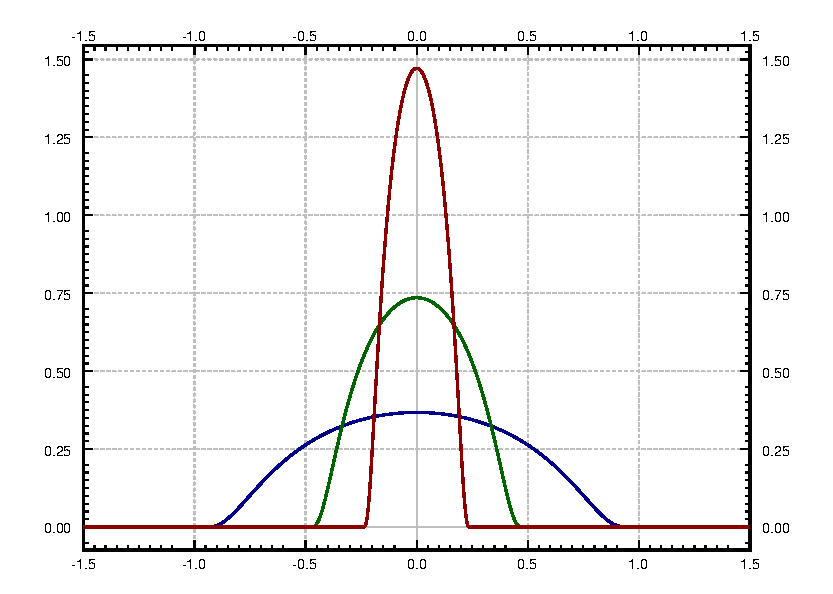
\includegraphics[width=3.0in]{figures/graph-of-mollifier.pdf}
\end{myfig}

First $f$ is bounded above on compact sets as it is upper semicontinuous.
If $f$ is not bounded below, we replace $f$ with $\max \{ f , 1/\epsilon
\}$, which is still plurisubharmonic.  Therefore, without loss of generality
we assume that $f$ is locally bounded.

For $z \in U_\epsilon$, we define $f_\epsilon$ as
the convolution with $g_\epsilon$:
\glsadd{not:convolution}%
\begin{equation*}
f_\epsilon(z) = (f * g_\epsilon)(z) =
\int_{\C^n} f(w) g_\epsilon (z-w) \, dV(w) =
\int_{\C^n} f(z-w) g_\epsilon (w) \, dV(w) .
\end{equation*}
The two forms of the integral follow easily via change of variables.
We are perhaps abusing notation a bit since $f$ is only defined on $U$,
but it is not a problem as long as $z \in
U_\epsilon$.
By differentiating the first form under the integral, $f_\epsilon$ is smooth.
Let us show that $f_\epsilon$ is plurisubharmonic.  We need to restrict to a
line $\xi \mapsto a+b\xi$.
We may translate and rotate by unitary matrices without affecting the setup.
So without loss of generality, suppose that $a = 0$, $b = (1,0,\ldots,0)$,
and that we are testing subharmonicity on a disc of radius $r$ around $\xi = 0$.
\begin{equation*}
\begin{split}
\frac{1}{2\pi} \int_0^{2\pi} f_\epsilon(re^{i\theta},0,\ldots,0)\, d\theta & =
\frac{1}{2\pi} \int_0^{2\pi}
\int_{\C^n}
f(re^{i\theta}-w_1,-w_2,\ldots,-w_n) g_\epsilon (w) \, dV(w) 
\,d\theta
\\
& =
\int_{\C^n}
\left(
\frac{1}{2\pi} \int_0^{2\pi}
f(re^{i\theta}-w_1,-w_2,\ldots,-w_n) \, d\theta \right) g_\epsilon (w) \, dV(w) 
\\
& \geq 
\int_{\C^n}
f(-w_1,-w_2,\ldots,-w_n) g_\epsilon (w) \, dV(w)  = f_\epsilon(0).
\end{split}
\end{equation*}
For the inequality we used $g_\epsilon \geq 0$.
So $f_\epsilon$ is plurisubharmonic.

As $g_\epsilon(w)$ only depends on $\sabs{w_1},\ldots,\sabs{w_n}$, we notice
that
$g_\epsilon(w_1,\ldots,w_n) =
g_\epsilon(\sabs{w_1},\ldots,\sabs{w_n})$.
Without loss of generality we consider $z=0$:
\begin{equation*}
\begin{split}
f_\epsilon(0)
& =
\int_{\C^n} f(-w) g_\epsilon (\sabs{w_1},\ldots,\sabs{w_n})
\, dV(w)
\\
& =
\int_0^\epsilon \cdots
\int_0^\epsilon
\left(
\int_0^{2\pi}
\cdots
\int_0^{2\pi}
 f(-r_1e^{i\theta_1},\ldots,
-r_ne^{i\theta_n}) \,
d\theta_1 \cdots d\theta_n \right)
\\
& \phantom{=}\qquad
g_\epsilon (r_1,\ldots,r_n) \,
 r_1 \cdots r_n \,d r_1 \cdots d r_n
\\
& \geq
\int_0^\epsilon \cdots
\int_0^\epsilon
\left(
\int_0^{2\pi}
\cdots
\int_0^{2\pi}
(2\pi)
 f(0,-r_2e^{i\theta_2},\ldots,
-r_ne^{i\theta_n}) \,
d\theta_2 \cdots d\theta_n \right)
\\
& \phantom{=}\qquad
g_\epsilon (r_1,\ldots,r_n) \,
 r_1 \cdots r_n \,d r_1 \cdots d r_n
\\
& \geq
f(0)
\int_0^\epsilon \cdots
\int_0^\epsilon
{(2\pi)}^n
g_\epsilon (r_1,\ldots,r_n) \,
 r_1 \cdots r_n \,d r_1 \cdots d r_n
\\
& = f(0) \int_{\C^n} g_\epsilon (w) d(w)
\\
& = f(0) .
\end{split}
\end{equation*}
The second equality above
follows because integral of $g_\epsilon$ only needs to be
done over the polydisc of radius $\epsilon$.
The penultimate equality follows from the fact that
$2\pi = \int_0^{2\pi}d \theta$.

We have $\limsup_{w\to z} f(w) = f(z)$ for subharmonic,
and therefore for plurisubharmonic functions.
Hence
for any $\delta >0$ find an $\epsilon
>0$ so that for $w \in B_\epsilon(0)$ we get $f(w)-f(0) \leq \delta$.
\begin{equation*}
\begin{split}
f_\epsilon(0) - f(0)
& =
\int_{B_\epsilon(0)} \bigl(f(-w)-f(0)\bigr)\, g_\epsilon (w)
\, dV(w)
\\
& \leq
\delta
\int_{B_\epsilon(0)} g_\epsilon (w)
\, dV(w)
= \delta .
\end{split}
\end{equation*}
Again we used that $g_\epsilon$ is nonnegative.
\end{proof}

\pagebreak[2]
\begin{exbox}
\begin{exercise}
Show that $g$ in the proof above is smooth on all of $\C^n$.
\end{exercise}

\begin{exercise}
\begin{exparts}
\item
Show that for a subharmonic function $\int_0^{2\pi} f(a+re^{i\theta}) \,
d\theta$ is a monotone function of $r$ (Hint: Try a $C^2$ function first and
use Green's theorem).
\item
Use this
fact to show that $f_\epsilon(z)$ from \thmref{thm:subharlim} are monotone
decreasing in $\epsilon$.
\end{exparts}
\end{exercise}

\begin{exercise}
If $g \colon U \subset \C^n \to V \subset \C^m$ is holomorphic and $f
\colon V \to \R$ is a $C^2$ plurisubharmonic function, then 
$f \circ g$ is plurisubharmonic.
Then use this to show that
this holds for all plurisubharmonic functions (Hint: monotone convergence).
\end{exercise}

\begin{exercise}
Show that plurisubharmonicity is a local property, that is,
$f$ is plurisubharmonic if and only if $f$ is plurisubharmonic in
some neighborhood of each point.
\end{exercise}

\begin{exercise}
Use the computation from
\thmref{thm:subharlim} to show that if $f$ is pluriharmonic, then
$f_\epsilon = f$ (where that makes sense), therefore obtaining another proof that 
a pluriharmonic function is $C^\infty$.
\end{exercise}

\begin{exercise}
Let the $f$ in \thmref{thm:subharlim} be continuous and suppose $K \subset
\subset U$, in particular for small enough $\epsilon >0$, $K \subset U_\epsilon$.
Show that $f_\epsilon$ converges uniformly to $f$ on $K$.
\end{exercise}

\begin{exercise}
Let the $f$ in \thmref{thm:subharlim} be $C^k$ for some $k \geq 0$.
Show that all derivatives of $f_\epsilon$ up to order $k$ converge uniformly
on compact sets to the corresponding derivatives of $f$.  See also previous
exercise.
\end{exercise}
\end{exbox}

As an application of harmonic functions, let us prove 
another useful theorem about zero sets of holomorphic functions,
the theorem of
Rad\'o.  It is sometimes covered in a one-variable course, but it is often
skipped.  It is very useful in several variables and the proof is a direct
application of the one-variable theory.
It is really a complementary theorem to the
Riemann extension theorem, when on the one hand the function is
continuous and vanishes on the set you wish to extend across, but on the
other hand you know nothing about this set.

\begin{thm}[Rad\'o] \index{Rad\'o's theorem}\label{thm:rado}
Let $U \subset \C^n$ be an open set and $f \colon U \to \C$ be a continuous
function that is holomorphic on the set
\begin{equation*}
U' = \{ z \in U : f(z) \not= 0 \} .
\end{equation*}
Then $f \in \sO(U)$.
\end{thm}

\begin{proof}
First assume $n=1$.  As the theorem is local, it is
enough to prove it for a small disc $\Delta$ such that $f$ is continuous
on the closure $\overline{\Delta}$, let $\Delta'$ be the part of the disc
where $f$ is nonzero as before.  If $\Delta'$ is empty, then we are done as
$f$ is just identically zero and hence holomorphic.

%Let us first show $\overline{\Delta'} = \overline{\Delta}$. Suppose
%the zero set of $f$ on $\Delta$ has interior.  Without loss of generality
%after composing with an automorphism of the disc

Let $u$ be the real part of $f$.  On $\Delta'$, $u$ is a harmonic function.
Let $Pu$ be the Poisson integral of $u$ on $\Delta$.  Hence $Pu$
equals $u$ on $\partial \Delta$, and $Pu$ is harmonic in all of $\Delta$.
Consider the function
$Pu(z) - u(z)$ on $\overline{\Delta}$.  The function is zero
on $\partial \Delta$ and it is harmonic on $\Delta'$.  By rescaling $f$
we can without loss of generality assume that $\abs{f(z)} < 1$ for all $z
\in \overline{\Delta}$.  For any $t >0$, the function 
$z \mapsto t \log \abs{f(z)}$ is subharmonic on $\Delta'$ and
upper-semicontinuous on $\overline{\Delta'}$.  Further, it is negative
on $\partial \Delta$.  The function $z \mapsto -t \log \abs{f(z)}$ is
superharmonic on $\Delta'$,
lower-semicontinuous on $\overline{\Delta'}$ and positive on $\partial
\Delta$.  On the set where $f$ is zero, the two functions are $-\infty$ and
$\infty$ respectively.  Therefore we have
\begin{equation*}
t \log \abs{f(z)} \leq Pu(z)-u(z) \leq -t \log \abs{f(z)} .
\end{equation*}
on $\overline{\Delta}$ for all $t > 0$.  Fixing $z \in \Delta'$ and letting
$t \to 0$ shows that $Pu = u$ on $\Delta'$.  In the same way we find that if
$v$ is the imaginary part of $f$, $Pv = v$ on $\Delta'$.  So we find that
$\tilde{f} = Pu + i Pv$ equals $f$ on $\overline{\Delta'}$, which includes
$\partial \Delta$.
Let $W = \Delta \setminus \overline{\Delta'}$.  If
this open set is empty we are finished.  If it is not empty,
the continuous
function $\tilde{f}-f$ is zero on $\overline{\Delta'}$, which includes
the boundary of $\Delta$.  So $\tilde{f}-f$ is zero on $\partial W$.
As $f$ is zero on $W$ then $\tilde{f}-f$ is holomorphic on $W$ and
by the maximum principle it must be zero on $W$.  Thus
$\tilde{f} = f$ everywhere and we are done.  The theorem is proved for
$n=1$.

The extension of the proof to several variables is left as an exercise.
\end{proof}

\begin{exbox}
\begin{exercise}
Use the one-variable result to extend the theorem to several variables.
\end{exercise}
\end{exbox}

%%%%%%%%%%%%%%%%%%%%%%%%%%%%%%%%%%%%%%%%%%%%%%%%%%%%%%%%%%%%%%%%%%%%%%%%%%%%%%

\section{Hartogs pseudoconvexity}

It is worth it to mention explicitly that by the above
exercises, plurisubharmonicity is preserved under holomorphic mappings.
That is if $g$ is holomorphic and $f$ is plurisubharmonic, then
$f \circ g$ is plurisubharmonic.  In particular if $\varphi \colon \D \to
\C^n$ is an analytic disc and $f$ is plurisubharmonic in a neighborhood of
$\varphi(\D)$,
then $f \circ \varphi$ is subharmonic.

\begin{defn}
Let $\sF$ be a class of (extended\footnote{%
By extended reals we mean $\R \cup \{ -\infty,\infty\}$.})-real-valued functions defined on $U \subset \R^n$.  If $K
\subset U$, define $\widehat{K}$, the \emph{\myindex{hull}} of $K$ with
respect to $\sF$, as the set
\glsadd{not:Khat}%
\begin{equation*}
\widehat{K} \overset{\text{def}}{=} \Bigl\{ z \in U : f(z) \leq \sup_{w\in K} f(w)
\text{ for all $f \in \sF$ } \Bigr\} .
\end{equation*}

A domain $U$ is said to be \emph{convex with respect to $\sF$}\index{convex!with respect to $\sF$}
if for every $K \subset \subset U$, the hull $\widehat{K} \subset \subset U$.%
\footnote{Recall that $\subset \subset$ means relatively compact.}
\end{defn}

Clearly $K \subset \widehat{K}$.  The key is to show that $\widehat{K}$
is not ``too large'' for $U$.
Keep in mind that the functions in $\sF$ are defined on $U$, so $\widehat{K}$
depends on $U$ not just on $K$.  An easy mistake is to consider functions defined
on a larger set, obtaining a smaller $\sF$ and hence a larger
$\widehat{K}$.  Sometimes it is useful to write $\widehat{K}_{\sF}$ to
denote the dependence on $\sF$, especially when talking about several different
hulls.
%We will instead explicitly say so in words to avoid too much notation.
%and avoid having to say so in words, but we do not take this shortcut.

\begin{exbox}
\begin{exercise}
Show that a domain $U \subset \R^n$
is geometrically convex (that is, the line segment
between any two points in $U$ is contained in $U$) if and only if it is
convex with respect to the convex functions on $U$.
\end{exercise}

\begin{exercise}
Show that any domain $U \subset \R^n$ is convex with respect to real
polynomials.
% in real variables $x_1,\ldots,x_n$.  Hint: Weierstrass
%approximation theorem makes this easy. (would be too easy)
\end{exercise}
%
%\begin{exercise}[Easy]
%Show that if $\overline{\Delta} \subset U$ is a closed analytic disc, then
%$\Delta$ is a subset of the hull of $\partial \Delta$ with respect to the
%plurisubharmonic functions.
%\end{exercise}
\end{exbox}

\begin{thm}[Kotinuit\"atssatz---Continuity
principle\index{Kotinuit\"atssatz}\index{continuity principle}]
Suppose $U \subset \C^n$ is convex with respect to plurisubharmonic
functions,
then given any collection of closed analytic discs $\Delta_\alpha$
such that $\bigcup_\alpha \partial \Delta_\alpha \subset \subset U$,
we have
$\bigcup_\alpha \Delta_\alpha \subset \subset U$.
\end{thm}

Various similar theorems are named the \emph{continuity principle}.
Generally what they have in common is the family of analytic discs whose
boundaries stay inside the domain, and whose conclusion has to do
with extension of holomorphic functions, or domains of holomorphy.

\begin{proof}
Let $f$ be a plurisubharmonic function on $U$.  If $\varphi_\alpha \colon
\overline{\D} \to U$ is the holomorphic (in $\D$) mapping giving the closed
analytic disc, then $f \circ \varphi_\alpha$ is subharmonic.
By the maximum principle,
$f$ on $\Delta_\alpha$ must be less than or equal to the supremum
of $f$ on $\partial \Delta_\alpha$, so $\overline{\Delta_\alpha}$
is in the hull of 
$\partial \Delta_\alpha$.
In other words
$\bigcup_\alpha \Delta_\alpha$ is in the hull of
$\bigcup_\alpha \partial \Delta_\alpha$ and therefore 
$\bigcup_\alpha \Delta_\alpha \subset \subset U$ by convexity.
\end{proof}

Let us illustrate the failure of the continuity principle.  If the domain
is not convex with respect to plurisubharmonic functions, then you could have
discs (denoted by straight line segments) that approach the boundary as in
the following picture.  In the diagram the boundaries of the discs are
denoted by the dark dots at the end of the segments.

\begin{myfig}
\subimport*{figures/}{contprinc.pdf_t}
\end{myfig}

\begin{defn}
Let $U \subset \C^n$ be a domain.  An $f \colon U \to \R$ is an \emph{\myindex{exhaustion function}} for $U$ if
\begin{equation*}
\bigl\{ z \in U : f(z) < r \bigr\} \subset \subset U
\qquad \text{for every $r \in \R$.}
\end{equation*}

A domain $U \subset \C^n$ is
\emph{\myindex{Hartogs pseudoconvex}}\index{pseudoconvex}
%(or usually just \emph{\myindex{pseudoconvex}})
if
there exists a continuous plurisubharmonic exhaustion function.
The set
$\{ z \in U : f(z) < r \}$ is called the \emph{\myindex{sublevel set}} of
$f$,
or the $r$-\emph{sublevel set}.
\end{defn}

\begin{example}
The unit ball $\bB_n$ is Hartogs pseudoconvex.  The continuous
function
\begin{equation*}
z \mapsto - \log \bigl( 1-\snorm{z} \bigr) 
\end{equation*}
is an exhaustion function, and it is easy to
check directly that it is plurisubharmonic.
\end{example}

\begin{example}
The entire $\C^n$ is Hartogs pseudoconvex as $\snorm{z}^2$ is
a continuous plurisubharmonic exhaustion function.
Also, because $\snorm{z}^2$ is plurisubharmonic, then given any $K \subset \subset
\C^n$, the hull $\widehat{K}$ with respect to plurisubharmonic functions must 
be bounded.  In other words, $\C^n$ is convex with respect to
plurisubharmonic functions.
\end{example}

\begin{samepage}
\begin{thm}
Suppose $U \subsetneq \C^n$ is a domain.  The following are equivalent:
\begin{enumerate}[(i)]
\item \label{thm:pscvx:itemi}
$-\log \rho(z)$ is plurisubharmonic, where $\rho(z)$ is the distance from $z$
to $\partial U$.
\item \label{thm:pscvx:itemii}
$U$ has a continuous plurisubharmonic exhaustion function,
that is, $U$ is Hartogs pseudoconvex.
\item \label{thm:pscvx:itemiii}
$U$ is convex with respect to plurisubharmonic functions defined on $U$.
\end{enumerate}
\end{thm}
\end{samepage}

\begin{proof}
\ref{thm:pscvx:itemi}
$\Rightarrow$
\ref{thm:pscvx:itemii}:
If $U$ is bounded,
the function $-\log \rho(z)$ is clearly a continuous exhaustion function.
If $U$ is unbounded, take 
$z \mapsto \max \{ -\log \rho(z) , \snorm{z}^2 \}$.

\ref{thm:pscvx:itemii}
$\Rightarrow$
\ref{thm:pscvx:itemiii}:
Suppose $f$ is a continuous plurisubharmonic exhaustion function.
If $K \subset \subset U$, then for some $r$ we have
$K \subset \{ z \in U : f(z) < r \} \subset \subset U$.
But then by definition of the hull $\widehat{K}$ we have
$\widehat{K} \subset \{ z \in U : f(z) < r \} \subset \subset U$.

\ref{thm:pscvx:itemiii}
$\Rightarrow$
\ref{thm:pscvx:itemi}:
For $c \in \C^n$ with $\snorm{c}=1$, let us define
\begin{equation*}
\rho_c(z) =
\sup \bigl\{ \lambda > 0 :
z+ \lambda t c \in U \text{ for all $\sabs{t} < 1$} \bigr\} .
\end{equation*}
So $\rho_c(z)$ is the radius of the largest affine disc centered at $z$
in the direction $c$ that still lies in $U$.
As $\rho(z) = \inf_c \rho_c(z)$,
\begin{equation*}
- \log \rho(z) = \sup_{\snorm{c}=1} \bigl(-\log \rho_c(z)\bigr) .
\end{equation*}
If we prove that for any $a, b, c$ the function $\xi \mapsto -\log \rho_c(a+b\xi)$ is
subharmonic, then $\xi \mapsto - \log \rho(a+b\xi)$ is subharmonic and we are done.
Here is the setup, the disc is drawn as a line:
\begin{myfig}
\subimport*{figures/}{distfun-hartogs.pdf_t}
\end{myfig}

Suppose $\Delta \subset \C$ is a disc such that for all $\xi \in
\overline{\Delta}$, $a+b\xi \in U$.  We need to show that if there is a
harmonic function $u$ on $\Delta$ continuous up to the boundary such
that $- \log \rho_c(a+b\xi) \leq u(\xi)$ on $\partial \Delta$, then
the inequality holds on $\Delta$.  Let $u = \Re f$ for a holomorphic
function $f$.
%Let us also suppose that without loss of generality $\Delta =
%\D$, $a = 0$.
For $\xi \in \partial \Delta$ we have  $- \log \rho_c(a+b\xi) \leq \Re
f(\xi)$,
or in other words
\begin{equation*}
\rho_c(a+b\xi) \geq e^{-\Re f(\xi)} = \babs{e^{-f(\xi)}}.
\end{equation*}
Using the definition of $\rho_c(a+b\xi)$, the statement above is equivalent
to saying that whenever $\sabs{t} < 1$ then 
\begin{equation*}
(a+b\xi)+cte^{-f(\xi)} \in U .
\end{equation*}
This statement holds when $\xi \in \partial \Delta$.  If we prove that it also
holds for $\xi \in \Delta$, then we are finished.

We think of $\varphi_t(\xi) = 
(a+b\xi)+cte^{-f(\xi)}$ as a closed analytic disc with boundary inside
$U$.  We have a family of analytic discs, parametrized by $t$, whose boundaries are in
$U$ for all $t$ with $\sabs{t} < 1$.  For $t=0$ the entire disc is
inside $U$.  Take $t_0 < 1$ such that
$\varphi_t(\Delta) \subset U$ for all $t$ with $\sabs{t} < t_0$.
Then
\begin{equation*}
\bigcup_{\sabs{t} < t_0} \varphi_t(\partial \Delta)
\subset
\bigcup_{\sabs{t} \leq t_0} \varphi_t(\partial \Delta)
\subset \subset U ,
\end{equation*}
because continuous functions take compact sets to compact sets.
Convexity with respect to plurisubharmonic  functions implies 
\begin{equation*}
\bigcup_{\sabs{t} < t_0} \varphi_t(\Delta)
\subset \subset U .
\end{equation*}
Again by continuity we have $\varphi_t(\Delta) \subset \subset U$ for
all $t$ with $\sabs{t} = t_0$, and consequently it is true when $\sabs{t}$
is even slightly larger than $t_0$.
Hence $\varphi_t(\D) \subset U$
for all $t$ with $\sabs{t} < 1$.  Thus
$(a+b\xi)+cte^{-f(\xi)} \in U$ for all $\xi \in \Delta$ and all $\sabs{t} <
1$.  And this implies $\rho_c(a+b\xi) \geq e^{-\Re f(\xi)}$, which in
turn implies $-\log \rho_c(a+b\xi) \leq \Re f(\xi) = u(\xi)$, and
therefore $-\log \rho_c(a+b\xi)$ is subharmonic.
\end{proof}

\begin{exbox}
\begin{exercise}
Show that if domains $U_1 \subset \C^n$ and $U_2 \subset \C^n$ are Hartogs
pseudoconvex then so are all the topological components of $U_1 \cap U_2$.
\end{exercise}

\begin{exercise}
Show that if domains $U \subset \C^n$ and $V \subset \C^m$ are Hartogs
pseudoconvex then so is $U \times V$.
\end{exercise}

\begin{exercise}
Show that every domain $U \subset \C$ is Hartogs pseudoconvex.
\end{exercise}

\begin{exercise} \label{exercise:nestedunions}
Show that the union $\bigcup_j U_j$ of a nested sequence of Hartogs pseudoconvex
domains $U_{j-1} \subset U_j \subset \C^n$ is Hartogs pseudoconvex.
\end{exercise}

\begin{exercise}
Let $\R^2 \subset \C^2$ be naturally embedded (that is, it is the
set where $z_1$ and $z_2$ are real).  Show that the set $\C^2 \setminus
\R^2$ is not Hartogs pseudoconvex.
\end{exercise}

\begin{exercise} \label{exercise:biholHartogs}
Suppose $U,V \subset \C^n$ are biholomorphic domains.
Prove that $U$ is Hartogs pseudoconvex if and only if $V$ is
Hartogs pseudoconvex.
\end{exercise}
\end{exbox}

The statement corresponding to \exerciseref{exercise:nestedunions} on nested unions
for domains of holomorphy is
the \emph{\myindex{Behnke--Stein theorem}}, which follows using this exercise and the solution
of the Levi-problem.  Although historically Behnke--Stein was proved
independently and used to solve the Levi-problem.

\exerciseref{exercise:biholHartogs} says that (Hartogs) pseudoconvexity is a
biholomorphic invariant.  That is a good indication that we are looking at a
correct notion.  It also allows us to change variables to more convenient
ones when proving a specific domain is (Hartogs) pseudoconvex.

It is not immediately clear from the definition, but Hartogs pseudoconvexity
is a local property.

\begin{lemma}
A domain $U \subset \C^n$ is Hartogs pseudoconvex if and only if
for every point $p \in \partial U$ there exists a neighborhood $W$ of $p$
such that $W \cap U$ is Hartogs pseudoconvex.
\end{lemma}

\begin{proof}
One direction is trivial,
%follows by an exercise above.  If $U$ is Hartogs pseudoconvex
%we pick a Hartogs pseudoconvex $W$ and then $U \cap W$ must be Hartogs
%pseudoconvex.
so let us consider the other direction.  For $p \in \partial U$ let
$W$ be such that $U \cap W$
is Hartogs pseudoconvex.  By intersecting with a ball, which is
Hartogs pseudoconvex, we assume $W = B_r(p)$ (a ball centered at $p$).
Let $B = B_{r/2}(p)$.  For
any $z \in B \cap U$, the distance from $z$ to the boundary of $W \cap U$ is the same as
the distance to $\partial U$.  The setup is illustrated in the following
figure.  The part of the boundary $\partial U$ in $W$ is marked by a thick
black line, the part of the boundary of $\partial (W \cap U)$ that arises as
the boundary of $W$ is marked by a thick gray line.  A point $q \in B$ is
marked and a ball of radius $\nicefrac{r}{2}$ around $q$ is dotted.

\begin{myfig}
\subimport*{figures/}{hartogs-pseudoconvex-local.pdf_t}
\end{myfig}

No point of distance $\nicefrac{r}{2}$ from $q$ can be in $\partial W$, and 
the distance of $q$ to $\partial U$ is at most $\nicefrac{r}{2}$ as $p \in \partial U$
and $p$ is the center of $B$.
\glsadd{not:dist}%
Let $\operatorname{dist}(x,y)$ denote the
euclidean distance function\footnote{If either $x$ and/or $y$ are sets
of points we take the infimum of the euclidean distance over all the points.}.
Then for $z \in B \cap U$
\begin{equation*}
- \log \, \operatorname{dist}(z, \partial U) = 
- \log \, \operatorname{dist}\bigl(z, \partial (U \cap W)\bigr).
\end{equation*}
We know the right hand side is plurisubharmonic.  We have such a ball $B$ of
positive radius around every $p \in \partial U$, so we have a
plurisubharmonic
exhaustion function near the boundary.

If $U$ is bounded, then $\partial U$ is compact.  So there is some
$\epsilon > 0$ such that $- \log \, \operatorname{dist}(z, \partial U)$
is plurisubharmonic if $\operatorname{dist}(z, \partial U) < 2\epsilon$.
The function
\begin{equation*}
\varphi(z) = \max \bigl\{
- \log \, \operatorname{dist}(z, \partial U) , - \log \epsilon \bigr\} 
\end{equation*}
is a continuous plurisubharmonic exhaustion function.  The proof for
unbounded $U$ requires some function of $\snorm{z}^2$ rather than a constant
$\epsilon$,
and is left as an exercise.
\end{proof}

\begin{exbox}
\begin{exercise}
Finish the proof of the lemma for unbounded domains.
\end{exercise}
\end{exbox}



It may seem that we defined a totally different concept, but it turns
out that Levi and Hartogs pseudoconvexity are one and the same on domains
where both concepts make sense.

\begin{thm}
Let $U \subset \C^n$ be a domain with smooth boundary. 
Then $U$ is Hartogs pseudoconvex if and only if $U$ is Levi pseudoconvex.
\end{thm}

As a consequence of this theorem we say simply ``pseudoconvex'' and there
is no ambiguity.

\begin{proof}
%Let us first suppose $U$ is Hartogs pseudoconvex.
Suppose
$U \subset \C^n$ is a domain with smooth boundary that is not
Levi pseudoconvex at $p \in \partial U$.
As in
\thmref{thm:tomatocan}, change coordinates so that $p=0$ and $U$ is defined
by
\begin{equation*}
\Im z_n > - \sabs{z_1}^2 + \sum_{j=2}^{n-1} \epsilon_j \sabs{z_j}^2 + O(3) .
\end{equation*}
For some small fixed $\lambda > 0$, the
analytic discs defined by $\xi \mapsto (\lambda \xi, 0, \cdots, 0, is)$
are in $U$ for all small enough $s > 0$.  As the origin
is in their limit set,
%we found a family of analytic discs in $U$
%whose boundaries were uniformly a positive distance away from $\partial U$,
%but such that $p$ was in the limit set of their interiors.  In fact we found an entire
%Hartogs figure in $U$.  So
Kontinuit\"atssatz is not satisfied, and $U$ is not 
convex with respect to the plurisubharmonic functions.  Therefore 
$U$ is not Hartogs pseudoconvex.

Next suppose $U$ is Levi pseudoconvex.  Take any $p \in \partial U$.
After translation and rotation by a unitary, assume $p=0$ and
write the defining function $r$ as
\begin{equation*}
r(z,\bar{z}) = \varphi(z',\bar{z}',\Re z_n) - \Im z_n ,
\end{equation*}
where $z' = (z_1,\ldots,z_{n-1})$ and
$\varphi$ is $O(2)$ at the origin.
The condition of Levi pseudoconvexity says 
\begin{equation} \label{eq:psconvcond}
\sum_{j=1,\ell=1}^n
\bar{a}_j a_\ell \frac{\partial^2 r}{\partial \bar{z}_j \partial z_\ell} \Big|_q \geq 0 
\quad \text{whenever} \quad
\sum_{j=1}^n
a_j \frac{\partial r}{\partial z_j} \Big|_q = 0 ,
\end{equation}
for all $q \in \partial U$ near $0$.
If we translate $\partial U$ slightly in the $\Im z_n$ direction, we still
have a Levi pseudoconvex boundary.  That is, we
look at the hypersurface given by $r=s$ for a small real constant $s$.
The condition \eqref{eq:psconvcond} is 
satisfied for the function $r-s$ instead of $r$,
as $\frac{\partial r}{\partial z_j} =
\frac{\partial (r-s)}{\partial z_j}$ for all $j$ and the
complex Hessians of $r$ and $r-s$ are also equal.
So condition \eqref{eq:psconvcond} holds for $r$ for all $q \in U$ near $0$.
We will use $r$ to manufacture a plurisubharmonic exhaustion function, that
is one with a semidefinite Hessian.  Therefore, we already
have what we need in all but one direction.

Let $\nabla_z r(q) =
\Bigl(
\frac{\partial r}{\partial z_1}\Big|_q,\ldots,
\frac{\partial r}{\partial z_n}\Big|_q \Bigr)$ denote the gradient of $r$ in
the holomorphic directions only.
Given $q \in U$ near $0$,
decompose an arbitrary $c \in \C^n$ as $c = a+b$, where $a = (a_1,\ldots,a_n)$
satisfies
\begin{equation*}
\sum_{j=1}^n
a_j \frac{\partial r}{\partial z_j} \Big|_q = 
\blinnprod{a}{\overline{\nabla_z r(q)}}
=
0 .
\end{equation*}
Taking the orthogonal decomposition, $b$ is a scalar multiple of $\overline{\nabla_z r(q)}$.
Then by Cauchy--Schwarz we find
\begin{equation*}
\abs{\sum_{j=1}^n c_j \frac{\partial r}{\partial z_j} \Big|_q}
=
\abs{\sum_{j=1}^n b_j \frac{\partial r}{\partial z_j} \Big|_q}
=
\Babs{\blinnprod{b}{\overline{\nabla_z r(q)}}}
=
\snorm{b} \snorm {\nabla_z r(q)} .
\end{equation*}
As $\nabla_z r(0) = (0,\ldots,0,-\nicefrac{1}{2i})$, then for $q$ sufficiently near $0$ we have that
$\snorm{\nabla_z r(q)} \geq \nicefrac{1}{3}$.  Therefore for such $q$,
\begin{equation*}
\snorm{b} =
\frac{\abs{\sum_{j=1}^n c_j \frac{\partial r}{\partial z_j} \Big|_q}}{\snorm {\nabla_z r(q)}}
\leq
3 \abs{\sum_{j=1}^n c_j \frac{\partial r}{\partial z_j} \Big|_q}
.
\end{equation*}
As $c = a+b$ is the orthogonal decomposition we have that $\snorm{c} \geq
\snorm{b}$.

\pagebreak[1]
Next, let $M \geq 0$ be the operator norm of the Hessian matrix of $r$.
Again using Cauchy--Schwarz
\begin{equation*}
\begin{split}
\sum_{j=1,\ell=1}^n
\bar{c}_j c_\ell \frac{\partial^2 r}{\partial \bar{z}_j \partial z_\ell} \Big|_q 
& =
\sum_{j=1,\ell=1}^n
( \bar{a}_j + \bar{b}_j )  (a_\ell + b_\ell) \frac{\partial^2 r}{\partial \bar{z}_j \partial z_\ell} \Big|_q 
\\
& =
\sum_{j=1,\ell=1}^n
\bar{a}_j a_\ell \frac{\partial^2 r}{\partial \bar{z}_j \partial z_\ell} \Big|_q 
\\
& \phantom{=}~
+
\sum_{j=1,\ell=1}^n
\bar{b}_j c_\ell \frac{\partial^2 r}{\partial \bar{z}_j \partial z_\ell} \Big|_q 
+
\sum_{j=1,\ell=1}^n
\bar{c}_j  b_\ell \frac{\partial^2 r}{\partial \bar{z}_j \partial z_\ell} \Big|_q 
-
\sum_{j=1,\ell=1}^n
\bar{b}_j  b_\ell \frac{\partial^2 r}{\partial \bar{z}_j \partial z_\ell} \Big|_q 
\\
& \geq
\sum_{j=1,\ell=1}^n
\bar{a}_j a_\ell \frac{\partial^2 r}{\partial \bar{z}_j \partial z_\ell} \Big|_q 
-
M\snorm{b}\snorm{c}
-
M\snorm{c}\snorm{b}
-
M\snorm{b}^2
\\
& \geq
-
3 M\snorm{c}\snorm{b} .
\end{split}
\end{equation*}
Together with what we know about
$\snorm{b}$ we get:
\begin{equation*}
\sum_{j=1,\ell=1}^n
\bar{c}_j c_\ell \frac{\partial^2 r}{\partial \bar{z}_j \partial z_\ell} \Big|_q 
\geq -3M \snorm{c} \snorm{b} %=
%-M \frac{\snorm{c}\Babs{\sum_{j=1}^n c_j \frac{\partial r}{\partial z_j}
%\big|_q}}{\snorm{\nabla_z r (q)}}
\geq
-3^2 M \snorm{c}\abs{\sum_{j=1}^n c_j \frac{\partial r}{\partial z_j}
\Big|_q} .
\end{equation*}
For $z \in U$ sufficiently close to $0$ define
\begin{equation*}
f(z) = -\log \bigl(-r(z)\bigr) + A \snorm{z}^2 ,
\end{equation*}
where $A > 0$ is some constant we will choose later.
The log is there to make the function blow up as we approach the boundary
and the $A \snorm{z}^2$ is adding a constant diagonal matrix to the complex
Hessian of $f$, which we hope is enough to make it positive semidefinite.
Let us compute:
\begin{equation*}
\frac{\partial^2 f}{\partial \bar{z}_j \partial z_\ell}
=
\frac{1}{r^2}
\frac{\partial r}{\partial \bar{z}_j}
\frac{\partial r}{\partial z_\ell}
-
\frac{1}{r}
\frac{\partial^2 r}{\partial \bar{z}_j \partial z_\ell} 
+
A\delta_{j}^{\ell} ,
\end{equation*}
where $\delta_j^\ell$ is the Kronecker delta\footnote{%
Recall $\delta_j^\ell = 0$ if $j\not= \ell$ and $\delta_j^\ell = 1$ if $j =
\ell$.}.
Apply the complex Hessian of $f$ to $c$ (recall that $r$ is negative
on $U$ and so for $q \in U$, $-r = \sabs{r}$):
\begin{equation*}
\begin{split}
\sum_{j=1,\ell=1}^n
\bar{c}_j c_\ell \frac{\partial^2 f}{\partial \bar{z}_j \partial z_\ell} \Big|_q 
& =
\frac{1}{r^2}
\abs{
\sum_{\ell=1}^n
c_\ell
\frac{\partial r}{\partial z_\ell} \Big|_q
}^2
+
\frac{1}{\sabs{r}}
\sum_{j=1,\ell=1}^n
\bar{c}_j
c_\ell
\frac{\partial^2 r}{\partial \bar{z}_j \partial z_\ell} \Big|_q
+
A \snorm{c}^2
\\
& \geq
\frac{1}{r^2}
\abs{
\sum_{\ell=1}^n
c_\ell
\frac{\partial r}{\partial z_\ell} \Big|_q
}^2
-
\frac{3^2 M}{\sabs{r}}
\snorm{c}\abs{\sum_{j=1}^n c_j \frac{\partial r}{\partial z_j} \Big|_q} 
+
A \snorm{c}^2 .
\end{split}
\end{equation*}
Now comes a somewhat funky trick.
As a quadratic polynomial in $\snorm{c}$, the right hand side of the
inequality
is always nonnegative if $A > 0$ and the discriminant is negative or zero.
Let us set the discriminant to zero:
\begin{equation*}
0 = 
{\left(
\frac{3^2 M}{\sabs{r}}
\abs{\sum_{j=1}^n c_j \frac{\partial r}{\partial z_j} \Big|_q}
\right)}^2
- 4A 
\frac{1}{r^2}
\abs{
\sum_{\ell=1}^n
c_\ell
\frac{\partial r}{\partial z_\ell} \Big|_q
}^2 .
\end{equation*}
All the nonconstant terms go away and 
$A=\frac{3^4 M^2}{4}$.  Thus
\begin{equation*}
\sum_{j=1,\ell=1}^n
\bar{c}_j c_\ell \frac{\partial^2 f}{\partial \bar{z}_j \partial z_\ell} \Big|_q 
\geq 0.
\end{equation*}
In other words, the complex Hessian
of $f$ is positive semidefinite at all points $q \in U$ near $0$.
The function $f(z)$ goes to infinity as $z$ approaches $\partial U$.
So for every $t \in \R$, the $t$-sublevel set
(the set where $f(z) < t$) must be a positive
distance away from $\partial U$ near $0$.

We have a local continuous plurisubharmonic
exhaustion function for $U$ near $p$.  If we intersect
with a small ball $B$ centered at $p$, then we get that $U \cap B$ is
Hartogs pseudoconvex.  This is true at all
$p \in \partial U$, so $U$ is Hartogs pseudoconvex.
\end{proof}

%FIXME: Reinhardt/circular domains?

%%%%%%%%%%%%%%%%%%%%%%%%%%%%%%%%%%%%%%%%%%%%%%%%%%%%%%%%%%%%%%%%%%%%%%%%%%%%%%

\section{Holomorphic convexity}

\begin{defn}
Let $U \subset \C^n$ be a domain.  For a set $K \subset U$,
define the
\emph{\myindex{holomorphic hull}}
\glsadd{not:KhatU}%
\begin{equation*}
\widehat{K}_U \overset{\text{def}}{=} \Bigl\{ z \in U : \sabs{f(z)} \leq
\sup_{w\in K} \sabs{f(w)}
\text{ for all $f \in \sO(U)$}  \Bigr\} .
\end{equation*}
The domain $U$ is \emph{\myindex{holomorphically convex}} if whenever
$K \subset \subset U$, then $\widehat{K}_U \subset \subset U$.
In other words, $U$ is holomorphically convex if it is convex with
respect to moduli of holomorphic functions on $U$.\footnote{Sometimes simply
$\widehat{K}$ is used, but we use
$\widehat{K}_U$ to emphasize the dependence on $U$.}
\end{defn}


It is a simple exercise (see below) to show that a holomorphically convex
domain is Hartogs pseudoconvex.  The converse is the
Levi problem for Hartogs pseudoconvex domains and is considerably more
difficult.  The thing is that there are lots of plurisubharmonic functions
and they are easy to construct; we can even construct them locally and then
piece them together as we have already seen.  There are far fewer holomorphic functions, and clearly
we cannot just construct them locally and expect the pieces to somehow fit
together.

\begin{exbox}
\begin{exercise}
Prove that a holomorphically convex domain is Hartogs pseudoconvex.
See \exerciseref{exercise:modholplush}.
\end{exercise}

\begin{exercise}
Compute the hull
$\widehat{K}_{\D^n}$ of the set $K = \bigl\{ z \in \D^n : \sabs{z_j} =
\lambda_j \text{ for } j=1,\ldots,n \bigr\}$, where $0 \leq \lambda_j < 1$.
Prove that the unit polydisc is holomorphically convex.
\end{exercise}

\begin{exercise}
Prove that a geometrically convex domain $U \subset \C^n$
is holomorphically convex.
\end{exercise}

\begin{exercise}
Prove that the Hartogs figure is not holomorphically convex.
\end{exercise}

\begin{exercise}
Let $U \subset \C^n$ be a domain and $f \in \sO(U)$.  Show that if
$U$ is holomorphically convex then
$\widetilde{U} = \bigl\{ z \in U : f(z) \not= 0 \bigr\}$
is holomorphically convex.  
Hint: First see \exerciseref{exercise:connectedcomplement}.
\end{exercise}

\begin{exercise} \label{exercise:biholholconvex}
Suppose $U,V \subset \C^n$ are biholomorphic domains.
Prove that $U$ is holomorphically convex if and only if $V$ is
holomorphically convex.
\end{exercise}

\begin{exercise}
In the definition of holomorphic hull of $K$, replace $U$ with $\C^n$
and $\sO(U)$ with holomorphic polynomials on $\C^n$, to get the
\emph{\myindex{polynomial hull}} of $K$.  Prove that the polynomial hull of
$K \subset \subset \C^n$ is the same as the holomorphic hull $\widehat{K}_{\C^n}$.
\end{exercise}

\begin{exercise}
\begin{exparts}
\item Prove the Hartogs triangle $T$ (see \exerciseref{exercise:hartogstriangle})
is holomorphically convex.
\item Prove $T \cup B_{\epsilon}(0)$ (for a small enough $\epsilon > 0$) is
not holomorphically convex.
\end{exparts}
\end{exercise}

\begin{exercise}
Show that if domains $U_1 \subset \C^n$ and $U_2 \subset \C^n$ are
holomorphically convex
then so are all the topological components of $U_1 \cap U_2$.
\end{exercise}

\begin{exercise}[Behnke--Stein again]
\index{Behnke--Stein theorem}
Show that the union $\bigcup_j U_j$ of a nested sequence of holomorphically
convex domains $U_{j-1} \subset U_j \subset \C^n$ is holomorphically convex.
\end{exercise}
\end{exbox}

Using an above exercise we see that $\C^n$ is both holomorphically convex and
a domain of holomorphy.  In fact, these two notions are equivalent for all
other domains in $\C^n$.

\pagebreak[3]
\begin{thm}[Cartan--Thullen\index{Cartan--Thullen theorem}]
\label{thm:cartthul}
Let $U \subsetneq \C^n$ be a domain.  The following are equivalent:
\begin{enumerate}[(i)]
\item \label{thm:cartthul:domhol}
$U$ is a domain of holomorphy.
\item \label{thm:cartthul:disthull}
For all $K \subset \subset U$,
$\operatorname{dist}(K,\partial U) = \operatorname{dist}(\widehat{K}_U,\partial U)$.
\item \label{thm:cartthul:holconv}
$U$ is holomorphically convex.
\end{enumerate}
\end{thm}

\begin{proof}
Let us start with \eqref{thm:cartthul:domhol} $\Rightarrow$
\eqref{thm:cartthul:disthull}.  Suppose there is a $K \subset
\subset U$ with $\operatorname{dist}(K,\partial U) > \operatorname{dist}(\widehat{K}_U,\partial U)$.
After possibly a rotation by a unitary,
there exists a point $p \in \widehat{K}_U$ and a polydisc
$\Delta = \Delta_r(0)$ with polyradius $r = (r_1,\ldots,r_n)$ such that
$p + \Delta = \Delta_r(p)$ contains a point of $\partial U$, but
\begin{equation*}
K + \Delta = \bigcup_{q \in K} \Delta_r(q) \subset \subset U.
\end{equation*}

\begin{myfig}
\subimport*{figures/}{cart-thul-fig.pdf_t}
\end{myfig}

If $f \in \sO(U)$, then there is an $M > 0$ such that $\sabs{f} \leq M$ on
$K + \Delta$ as that is a relatively compact set.  By the Cauchy estimates
for each $q \in K$ we get
\begin{equation*}
\abs{\frac{\partial^\alpha f}{\partial z^\alpha}(q)} \leq \frac{M
\alpha!}{r^\alpha} .
\end{equation*}
This inequality therefore holds on $\widehat{K}_U$ and hence at $p$.
The series
\begin{equation*}
\sum_{\alpha}
\frac{1}{\alpha !}\frac{\partial^\alpha f}{\partial z^\alpha}(p) {(z-p)}^\alpha 
\end{equation*}
converges in $\Delta_r(p)$.  Hence $f$ extends to all of $\Delta_r(p)$ and
$\Delta_r(p)$ contains points outside of $U$, in other words,
$U$ is not a domain of holomorphy.

The implication \ref{thm:cartthul:disthull} $\Rightarrow$
\ref{thm:cartthul:holconv} is easy.

Finally let us prove
\ref{thm:cartthul:holconv} $\Rightarrow$
\ref{thm:cartthul:domhol}.
Suppose $U$ is holomorphically convex.  Let $p \in \partial U$.
By convexity we choose nested compact sets $K_{j-1} \subsetneq K_j \subset
\subset U$ such that $\bigcup_j K_j = U$, and $\widehat{(K_j)}_U = K_j$.
We pick the sequence of $K_j$ in such a way that 
there exists a 
sequence of points $p_j \in K_j \setminus K_{j-1}$ such that
$\lim_{j\to\infty} p_j = p$.

Since $p_j$ is not in the hull of $K_{j-1}$, we find a function $f_j \in
\sO(U)$ such that $\sabs{f_j} < 2^{-j}$ on $K_{j-1}$, but such that
\begin{equation*}
\sabs{f_j(p_j)} > j + \abs{\sum_{k=1}^{j-1} f_k(p_j)} .
\end{equation*}
Finding such a function is left as an exercise below.
The series $\sum_{k=1}^\infty f_k(z)$ converges uniformly on $K_j$
as for all $k > j$, $\sabs{f_k} < 2^{-k}$ on $K_j$.
As the $K_j$ exhaust $U$ the series converges uniformly on compact
subsets of $U$.  Consequently,
\begin{equation*}
f(z) = \sum_{k=1}^\infty f_k(z)
\end{equation*}
is a holomorphic function on $U$.  We bound
\begin{equation*}
\sabs{f(p_j)} \geq
\sabs{f_j(p_j)}
-
\abs{\sum_{k=1}^{j-1} f_k(p_j)}
-
\abs{\sum_{k=j+1}^\infty f_k(p_j)}
\geq
j
-
\sum_{k=j+1}^\infty 2^{-k}
\geq j-1 .
\end{equation*}
So $\lim_{j\to\infty} f(p_j) = \infty$.
Clearly there cannot be any open $W \subset \C^n$
containing $p$ to which $f$ extends (see definition of domain of holomorphy).  As any
connected open $W$ such that $W \setminus U \not= \emptyset$ must contain a
point of $\partial U$, we are done.
\end{proof}

\exerciseref{exercise:biholholconvex}
says that holomorphic convexity is a biholomorphic invariant.
Therefore,
being a domain of holomorphy is also a biholomorphic invariant.  This
fact is not easy to prove directly from the definition of a domain of
holomorphy, as the
biholomorphism is only defined on the interior of our domains.

Holomorphic convexity is an intrinsic notion; that is, it does not require
knowing anything about points outside of $U$.  Therefore, it is a much
better way to think about domains of holomorphy.  In fact holomorphic
convexity generalizes easily to more complicated complex
manifolds\footnote{Manifolds with complex structure, that is, ``manifolds
with multiplication by $i$ on the tangent space''.}, while
the notion of a domain of holomorphy only makes sense in $\C^n$.

\begin{exbox}
\begin{exercise}
Find the function $f_j \in \sO(U)$ as indicated in the proof above.
\end{exercise}

\begin{exercise}
Extend the proof to show that if $U \subset \C^n$
is holomorphically convex then there
exists a single function $f \in \sO(U)$, that does not extend through any
point $p \in \partial U$.
\end{exercise}
\end{exbox}

%%%%%%%%%%%%%%%%%%%%%%%%%%%%%%%%%%%%%%%%%%%%%%%%%%%%%%%%%%%%%%%%%%%%%%%%%%%%%%
%%%%%%%%%%%%%%%%%%%%%%%%%%%%%%%%%%%%%%%%%%%%%%%%%%%%%%%%%%%%%%%%%%%%%%%%%%%%%%
%%%%%%%%%%%%%%%%%%%%%%%%%%%%%%%%%%%%%%%%%%%%%%%%%%%%%%%%%%%%%%%%%%%%%%%%%%%%%%

\chapter{CR geometry} \label{ch:crgeometry}

%%%%%%%%%%%%%%%%%%%%%%%%%%%%%%%%%%%%%%%%%%%%%%%%%%%%%%%%%%%%%%%%%%%%%%%%%%%%%%

\section{Real analytic functions and complexification}

\begin{defn}
Let $U \subset \R^n$ be open.
A function $f \colon U \to \C$ is 
\emph{\myindex{real-analytic}} (or simply \emph{analytic} if
clear from context) if at each point $p \in U$, the function $f$
has a convergent power series that converges (absolutely) to $f$ in some
neighborhood of $p$.
\glsadd{not:Comega}%
A common notation for real-analytic is $C^\omega$.
\end{defn}

Before we discuss the connection to holomorphic functions let us prove a simple
lemma.

\begin{lemma}
Let $\R^n \subset \C^n$ be the natural inclusion and suppose
$U \subset \C^n$ is a domain such that $U \cap \R^n \not= \emptyset$.
Suppose $f,g \colon U \to \C$ be holomorphic functions such that
$f=g$ on $U \cap \R^n$.  Then $f=g$ on all of $U$.
\end{lemma}

\begin{proof}
By taking $f-g$ we can assume that $g=0$.
Let $z = x+iy$ as usual so that $\R^n$ is given by $y=0$.
Our assumption is that $f = 0$ when $y=0$,
so the derivative of $f$ with respect to $x_j$ is zero.
So when $y=0$,
the Cauchy--Riemann equations say
\begin{equation*}
0 = \frac{\partial f}{\partial x_j} =
-i \frac{\partial f}{\partial y_j} .
\end{equation*}
Therefore, on $y=0$,
\begin{equation*}
\frac{\partial f }{\partial z_j} = 0 .
\end{equation*}
The derivative $\frac{\partial f }{\partial z_j}$ is holomorphic
and $\frac{\partial f }{\partial z_j} = 0$ on $y=0$.  Then
by induction all derivatives of $f$ at $p \in \R^n \cap U$ vanish, it has a zero 
power series.  Hence $f$ is identically zero in a neighborhood of
$p$ in $\C^n$ and by the identity theorem it is zero on all of $U$.
\end{proof}


Let us return to $\R^n$ for a moment.
We write a power series in $\R^n$ in multinomial notation as usual.
Suppose that for some
$a \in \R^n$
and some polyradius
$r=(r_1,\ldots,r_n)$,
the series
\begin{equation*}
\sum_{\alpha} c_{\alpha} {(x-a)}^\alpha
\end{equation*}
converges whenever $\sabs{x_j-a_j} \leq r_j$ for all $j$.
Here convergence is absolute convergence.  That is,
\begin{equation*}
\sum_{\alpha} \sabs{c_{\alpha}}\, \sabs{x-a}^\alpha
\end{equation*}
converges.
If we replace $x_j \in \R$ with $z_j \in \C$ such that
$\sabs{z_j-a_j} \leq \sabs{x_j-a_j}$, then the series still converges.
Hence the series
\begin{equation*}
\sum_{\alpha} c_{\alpha} {(z-a)}^\alpha
\end{equation*}
converges absolutely in $\Delta_r(a) \subset \C^n$.

\begin{prop}[Complexification part I\index{complexification}]
Suppose $U \subset \R^n$ is a domain and
$f \colon U \to \C$ is real-analytic.
Let $\R^n \subset \C^n$ be the natural inclusion.
Then there exists a domain $V \subset \C^n$ such that $U \subset V$
and a unique holomorphic function $F \colon V \to \C$ such that $F|_U = f$.
\end{prop}

In particular, among many other things that follow from this proposition, we
can now conclude that a real-analytic function is $C^\infty$.  Be careful
and notice that $U$ is a domain in $\R^n$, but it is not an open set
when considered as a subset of $\C^n$.  Furthermore, $V$ may be a very
``thin'' neighborhood around $U$.  There is no way of finding $V$ just from
knowing $U$.  You need to also know $f$.
As an example, consider
$f(x) = \frac{1}{\epsilon^2+x^2}$ for $\epsilon > 0$, which is
real-analytic on $\R$, but the complexification is not holomorphic at $\pm
\epsilon i$.

\begin{proof}
We already proved the local version.  But we must prove that if we
extend our $f$ near every point, we always get the same function.
That follows from the lemma above; any two such functions are
equal on $\R^n$, and hence equal.  There is a subtle topological technical
point in this, so let us elaborate.  A key topological fact is that we define
$V$ as a union of the polydiscs where the series converges.  If there was a
point where we get two distinct values, then this point must be in two
distinct such polydiscs.  The intersection of two polydiscs is always
connected, so we can apply the lemma above.
\end{proof}

Recall that a polynomial $P(x)$ in $n$ real variables $(x_1,\ldots,x_n)$ is homogeneous of degree $d$ if
$P(s x) = s^d P(x)$ for all $s \in \R$ and $x \in \R^n$.
That is, a homogeneous polynomial of degree $d$ is a polynomial whose
every monomial
is of total degree $d$.
%  For example, $x^2y-iy^3+9xy^2$ is homogeneous of
%degree 3.
If $f$ is real-analytic near $a \in \R^n$, then
write the power series of $f$ at $a$ as
\begin{equation*}
\sum_{j=0}^{\infty} f_j(x-a) ,
\end{equation*}
where $f_j$ is a homogeneous polynomial of degree $j$.  The $f_d$ is then
called the
\emph{\myindex{degree $d$ homogeneous part}}\index{homogeneous part} of $f$
at $a$.

When dealing with real-analytic functions in $\C^n$, there is usually a better
way to complexify.
Suppose $U \subset \C^n \cong \R^{2n}$, and suppose $f \colon U \to
\C$ is real-analytic.  Let us assume that $a=0$ for simplicity.
Writing $z = x+iy$,
\begin{equation*}
f(x,y)
= 
\sum_{j=0}^\infty
f_j(x,y)
= 
\sum_{j=0}^\infty
f_j\left(
\frac{z+\bar{z}}{2},
\frac{z-\bar{z}}{2i}\right) .
\end{equation*}
The polynomial $f_j$ becomes a homogeneous polynomial of degree $j$
in the variables $z$ and $\bar{z}$.  Therefore the entire
series becomes a power series in $z$ and $\bar{z}$.  As we mentioned before,
we simply write $f(z,\bar{z})$, and when we consider the
power series representation it will be in $z$ and $\bar{z}$ rather than
in $x$ and $y$.
In multinomial notation we write a power series at $a \in \C^n$ as
\begin{equation*}
\sum_{\alpha,\beta} c_{\alpha,\beta} {(z-a)}^\alpha
{(\bar{z}-\bar{a})}^\beta .
\end{equation*}

Notice that a holomorphic function
is real-analytic, but not vice-versa.  A holomorphic function
is a real-analytic function that does not depend on $\bar{z}$.

Before we discuss complexification in terms of $z$ and $\bar{z}$ we need
the following lemma.

\begin{lemma}
Let $U \subset \C^n \times \C^n$ be a domain, let the coordinates be $(z,\zeta) \in \C^n \times
\C^n$, let
\begin{equation*}
D = \bigl\{ (z,\zeta) \in \C^n \times \C^n : \zeta = \bar{z} \bigr\},
\end{equation*}
and suppose $D \cap U \not= \emptyset$.
Suppose $f,g \colon U \to \C$ be holomorphic functions such that
$f=g$ on $D \cap U$.  Then $f=g$ on all of $U$.
\end{lemma}

The set $D$ is sometimes called the \emph{\myindex{diagonal}}.

\begin{proof}
Again assume without loss of generality that $g=0$.
Whenever $(z,\bar{z}) \in U$, we have $f(z,\bar{z}) = 0$, which is really
$f$ composed with the map that takes $z$ to $(z,\bar{z})$.  Using the chain rule
\begin{equation*}
0 =
\frac{\partial}{\partial \bar{z}_j} \bigl(f(z,\bar{z})\bigr)
=
\frac{\partial f}{\partial \zeta_j}(z,\bar{z}) .
\end{equation*}
Let us do this again with the $z_j$
\begin{equation*}
0 =
\frac{\partial}{\partial z_j} \bigl(f(z,\bar{z})\bigr)
=
\frac{\partial f}{\partial z_j}(z,\bar{z}) .
\end{equation*}
Each time we get another holomorphic function that is zero on $D$.
By induction, for all $\alpha$ and $\beta$ we get
\begin{equation*}
0 =
\frac{\partial^{\sabs{\alpha}+\sabs{\beta}}}{\partial z^\alpha \partial \bar{z}^\beta} \bigl(f(z,\bar{z})\bigr)
=
\frac{\partial^{\sabs{\alpha}+\sabs{\beta}} f}{\partial z^\alpha \partial
\zeta^\beta}(z,\bar{z}) .
\end{equation*}
Therefore all holomorphic derivatives of $f$ are zero on every point
$(z,\bar{z})$.  So $f$ must be identically zero in a neighborhood of any
point $(z,\bar{z})$.  The lemma follows by the identity
theorem.
\end{proof}

Let $f$ be a real-analytic function.  Suppose 
the series (in multinomial notation)
\begin{equation*}
f(z,\bar{z}) =
\sum_{\alpha,\beta} c_{\alpha,\beta} {(z-a)}^\alpha
{(\bar{z}-\bar{a})}^\beta
\end{equation*}
converges in a polydisc $\Delta_r(a) \subset \C^n$.
By convergence we mean absolute
convergence as we discussed before: that is,
\begin{equation*}
\sum_{\alpha,\beta} \sabs{c_{\alpha,\beta}} \, \sabs{z-a}^\alpha
\sabs{\bar{z}-\bar{a}}^\beta
\end{equation*}
converges.
Therefore the series still converges if we replace $\bar{z}_j$  with
$\zeta_j$ where $\sabs{\zeta_j-\bar{a}} \leq \sabs{\bar{z}_j-\bar{a}}$.
So the series
\begin{equation*}
F(z,\zeta) =
\sum_{\alpha,\beta} c_{\alpha,\beta} {(z-a)}^\alpha
{(\zeta-\bar{a})}^\beta
\end{equation*}
converges for all $(z,\zeta) \in \Delta_r(a) \times \Delta_r(\bar{a})$.

Putting together the above with the lemma we obtain.

\begin{prop}[Complexification part II\index{complexification}] \label{prop:complexificationpt2}
Suppose $U \subset \C^n$ is a domain and $f \colon U \to \C$ is
real-analytic.
Then there exists a domain $V \subset \C^n \times \C^n$ such that
\begin{equation*}
\bigl\{ (z,\zeta) : \zeta = \bar{z} \text{ and } z \in U \bigr\} \subset V ,
\end{equation*}
and a unique holomorphic function $F \colon V \to \C$ such that
$F(z,\bar{z}) = f(z,\bar{z})$ for all $z \in U$.
\end{prop}

The function $f$ can be thought of as the restriction of $F$ to the set
where $\zeta = \bar{z}$.  We will abuse notation and write
simply $f(z,\zeta)$ both for $f$ and its extension.

\begin{remark}
The domain $V$ above is not simply $U$ times the conjugate of $U$.  In
general it is much smaller.  For example a real-analytic $f \colon \C^n \to
\C$ does not necessarily complexify to all of $\C^n \times \C^n$.  That is
because the domain of convergence for a real-analytic function on $\C^n$
is not necessarily all of $\C^n$.  For example, in one dimension
the function
\begin{equation*}
f(z,\bar{z})
= \frac{1}{1+\sabs{z}^2}
\end{equation*}
is real-analytic on $\C$, but it is not a restriction to the diagonal
of a holomorphic function on all of $\C^2$.  The problem is that the complexified
function
\begin{equation*}
f(z,\zeta)
= \frac{1}{1+z \zeta}
\end{equation*}
cannot be defined along the set where $z \zeta = -1$, which by a fluke
never happens when $\zeta = \bar{z}$.
\end{remark}

\begin{remark}
This form of complexification is sometimes called
\emph{\myindex{polarization}} due to its relation to the polarization
identities\footnote{Such as $4 \linnprod{z}{w} =
\snorm{z+w}^2-\snorm{z-w}^2 +i \bigl( \snorm{z+iw}^2 - \snorm{z-iw}^2 \bigr)$.}.  That is, suppose $A$ is a Hermitian matrix, we 
recover $A$ and therefore the sesquilinear form $\linnprod{Az}{w}$ for
$z,w\in \C^n$, by simply knowing the values of
\begin{equation*}
\linnprod{Az}{z} = z^*Az = \sum_{j,k=1}^n a_{jk} \, \bar{z}_j z_k 
\end{equation*}
for all $z \in \C^n$.  In fact, under the hood \propref{prop:complexificationpt2} is
polarization in an infinite-dimensional Hilbert space, but we digress.
\end{remark}

The idea of treating $\bar{z}$ as a separate variable is very powerful, and
as we have just seen it is completely natural when speaking about
real-analytic functions.  This is one of the reasons why real-analytic
functions play a special role in several complex variables.

\begin{example}
Not every $C^\infty$ smooth function is real-analytic.  For example,
on the real line
\begin{equation*}
f(x) =
\begin{cases}
e^{-1/x^2} & \text{if $x > 0$,} \\
0 & \text{if $x \leq 0$.}
\end{cases}
\end{equation*}
The function
$f \colon \R \to \R$ is $C^\infty$ and $f^{(k)}(0) = 0$ for all $k$.
So the Taylor series of $f$ at the origin does
not converge to $f$ in any neighborhood of the origin.  It converges to the
zero function but not to $f$.
\end{example}

\begin{exbox}
\begin{exercise}
Prove the statements of the above example.
\end{exercise}
\end{exbox}

\begin{defn}
A real hypersurface $M \subset \R^n$ is said to be real-analytic
if locally at every point it is the graph of a real-analytic function.  That
is near every point (that is, locally), after perhaps a rotation $M$ can be written as
\begin{equation*}
y = \varphi(x) ,
\end{equation*}
where $\varphi$ is real-analytic.
\end{defn}

Compare this definition to \defnref{def:hypersurface}.  In fact, we could
define a real-analytic hypersurface as in 
\defnref{def:hypersurface} and then prove an analogue of
\lemmaref{lemma:realgraphcoords} to show that this would be identical to the
definition above.  The definition we gave will be sufficient and so we avoid
the complication and leave it to the interested reader.

\begin{exbox}
\begin{exercise}
Show that the definition above is equivalent to an analogue of
\defnref{def:hypersurface}.  That is, state the alternative definition of
real-analytic hypersurface and then prove the analogue of 
\lemmaref{lemma:realgraphcoords}.
\end{exercise}
\end{exbox}

A mapping to $\R^m$ is real-analytic if all the components are real-analytic
functions.  Via complexification we give a simple proof of the following
result.

\begin{prop}
Let $U \subset \R^n$, $V \subset \R^k$ be domains and let
$f \colon U \to V$ and $g \colon V \to \R^m$ be real-analytic.
Then $g \circ f$ is real-analytic.
\end{prop}

\begin{proof}
Let $x \in \R^n$ be our coordinates in $U$ and $y \in \R^k$ be
our coordinates in $V$.  We complexify $f(x)$ and $g(y)$ by
allowing $x$ to be a complex vector in a small neighborhood of $U$ in
$\C^n$
and  $y$ to be a complex vector in a small neighborhood of $V$ in $\C^k$.
So we treat $f$ and $g$ as holomorphic functions.  On a certain
neighborhood of $U$ in $\C^n$, the composition $f \circ g$ makes sense
and it is holomorphic as composition of holomorphic mappings is holomorphic.
Restricting the complexified $f \circ g$ back to $\R^n$ we obtain a
real-analytic function.
\end{proof}

The proof demonstrates a very simple application of complexification.  Many
properties of holomorphic functions are easy to prove because
holomorphic functions are solutions to certain PDE (the Cauchy--Riemann
equations).  However, there is no PDE
that defines real-analytic functions, so complexification provides a useful
tool to transfer certain properties of holomorphic functions to
real-analytic functions.  We must be careful however, hypotheses on
real-analytic functions only give us hypotheses on certain points of the
complexified holomorphic functions.

\begin{exbox}
\begin{exercise}
Suppose $\varphi \colon U \to \R$ is a pluriharmonic function for $U \subset
\C^n$.  Knowing that $\varphi$ is real-analytic, let $z_0 \in U$ be fixed.
Using complexification, write down a formula for a holomorphic function near
$z_0$ whose real part is $\varphi$.
\end{exercise}
\end{exbox}

%%%%%%%%%%%%%%%%%%%%%%%%%%%%%%%%%%%%%%%%%%%%%%%%%%%%%%%%%%%%%%%%%%%%%%%%%%%%%%

\section{CR functions}

We first need to know what it means for a function $f \colon X \to \C$
to be smooth if $X$ is not an open set, for example, if $X$ is a hypersurface.

\begin{defn}
Let $X \subset \R^n$ be a set.
The function $f \colon X \to \C$ is smooth (resp.\
real-analytic) if for each point $p \in X$ there is a
neighborhood $U \subset \R^n$ of $p$ and a smooth (resp.\ real-analytic) $F
\colon U \to \C$ such that $F(q) = f(q)$ for $q \in X \cap U$.
\end{defn}

For an arbitrary set $X$, issues surrounding this definition can be very subtle.  It
is very natural, however, if $X$ is nice, such as a hypersurface, or if $X$ is
a closure of a domain with smooth boundary.

\begin{prop}
If $M \subset \R^n$ is a smooth (resp.\ real-analytic) real hypersurface, then $f \colon M \to \C$
is smooth (resp.\ real-analytic) if and only if whenever near some point we write $M$
as
\begin{equation*}
y = \varphi(x)
\end{equation*}
for a smooth (resp.\ real-analytic) function $\varphi$, then
the function $f\bigl(x,\varphi(x)\bigr)$ is a smooth (resp.\ real-analytic) function of $x$.
\end{prop}

\begin{exbox}
\begin{exercise}
Prove the proposition above.
\end{exercise}

\begin{exercise}
Prove that in the definition if $X$ is a smooth or real-analytic
hypersurface, then the function $F$ from the definition is never unique,
even for a fixed neighborhood $U$.
\end{exercise}
\end{exbox}

\begin{defn}
Let $M \subset \C^n$ be a smooth real hypersurface.  Then
a smooth function $f \colon M \to \C$ is a
\emph{\myindex{smooth CR function}}\index{CR function} if
\begin{equation*}
X_p f = 0
\end{equation*}
for all $p \in M$ and all vectors $X_p \in T^{(0,1)}_p M$.
\end{defn}

\begin{remark}
Of course one only needs one-derivative in the above definition.  One can also
define a continuous CR function if the derivative is taken in the
distribution sense, but we digress.
\end{remark}

\begin{remark}
When $n=1$, a real hypersurface $M \subset \C$ is a curve and $T^{(0,1)}_p M$
is trivial.  Therefore, all functions are CR functions.
\end{remark}

\begin{prop}
Let $M \subset U$ be a smooth (resp.\ real-analytic) real hypersurface in a domain $U
\subset \C^n$.  Suppose $F \colon U \to \C$ is a holomorphic function,
then the restriction $f = F|_M$ is a smooth (resp.\ real-analytic) CR function.
\end{prop}

\begin{proof}
First let us prove that $f$ is smooth.  Given any $p \in M$ write $M$
as $\Im w = \varphi(z,\bar{z},\Re w)$ for a smooth $\varphi$.
Then $F\bigl(z,\Re w + i \varphi(z,\bar{z},\Re w) \bigr)$
is clearly smooth as it is a composition of smooth functions.
If both $M$ and $\varphi$ are real-analytic, we obtain that 
$F\bigl(z,\Re w + i \varphi(z,\bar{z},\Re w) \bigr)$ is real-analytic, which
we could also prove directly by complexifying as before.

Let us show it is CR\@.
We have $X_p F = 0$
for all $X_p \in T_p^{(0,1)} \C^n$.
As $T_p^{(0,1)} M \subset T_p^{(0,1)} \C^n$ we have
$X_p f = 0$ for all $X_p \in T_p^{(0,1)} M$.
\end{proof}

Not every smooth CR function is a restriction of a holomorphic function.

\begin{example}
Take the smooth function $f \colon \R \to \R$ we defined before
that is not real-analytic at the origin.
Take $M \subset \C^2$ be the set defined by $\Im z_2 = 0$, this is a
real-analytic real hypersurface.  Clearly
$T_p^{(0,1)} M$ is one-complex-dimensional and at each point
$\frac{\partial}{\partial \bar{z}_1}$ is tangent and therefore spans
$T_p^{(0,1)} M$.  Define $g \colon M \to \C$ by
\begin{equation*}
g(z_1,z_2,\bar{z}_1,\bar{z}_2) = f(\Re z_2) .
\end{equation*}
Then $g$ is CR as it is independent of $\bar{z}_1$.
If $G \colon U \subset \C^2 \to \C$ is a holomorphic
function where $U$ is some open set containing the origin, then $G$
restricted to $M$ must be real-analytic (a power series in $\Re z_1$, $\Im
z_1$, and $\Re z_2$) and therefore $G$ cannot equal to 
$g$ on $M$.
\end{example}

\begin{exbox}
\begin{exercise}
Suppose $M \subset \C^n$ is a smooth hypersurface
and $f \colon M \to \C$ is a CR function that is a restriction
of a holomorphic function $F \colon U \to \C$ defined in
some neighborhood $U \subset \C^n$ of $M$.  Show that $F$ is unique,
that is if $G \colon U \to \C$ is another holomorphic function such that
$G|_M = f = F|_M$, then $G=F$.
\end{exercise}

\begin{exercise}
Show that there is no maximum principle of CR functions.  In fact, find a
smooth hypersurface $M \subset \C^n$, $n \geq 2$, and a smooth CR function
$f$ on $M$ such that $\sabs{f}$ attains a strict maximum at a point.
\end{exercise}

\begin{exercise}
Suppose $M \subset \C^n$, $n \geq 2$, is the hypersurface given by $\Im z_n
= 0$.  Show that any smooth CR function on $M$ is holomorphic in the variables
$z_1,\ldots,z_{n-1}$.  Use this to show that for no smooth CR function $f$ on $M$ can
$\sabs{f}$ attain a \emph{strict} maximum on $M$.  But show that there do
exist functions such that $\sabs{f}$ attains a (nonstrict) maximum $M$.
\end{exercise}
\end{exbox}

Real-analytic CR functions on a real-analytic
hypersurface $M$ always extend to holomorphic functions of a neighborhood of $M$.
Before we prove that fact, let us find a convenient way to write the defining
equation for a real-analytic hypersurface.

\begin{prop}
Suppose $M \subset \C^n$ is a real-analytic hypersurface and $p \in M$.
Then there are holomorphic coordinates near $p$ taking $p$ to 0,
such that locally $M$ is given by
\begin{equation*}
\bar{w} = \Phi(z,\bar{z},w) ,
\end{equation*}
for a holomorphic function $\Phi$ defined on a neighborhood of the origin
in $\C^{n-1} \times \C^{n-1} \times \C$ that is $O(2)$ at the origin.
Furthermore, a local basis for $T^{(0,1)} M$ vector fields is given by
\begin{equation*}
\frac{\partial}{\partial \bar{z}_j}
+\frac{\partial \Phi}{\partial \bar{z}_j} \frac{\partial}{\partial \bar{w}} ,
\qquad j=1,\ldots,n-1.
\end{equation*}
\end{prop}

\begin{proof}
Find coordinates such that $M$ is given by
\begin{equation*}
\Im w = \varphi(z,\bar{z},\Re w) .
\end{equation*}
Write the defining function
as $r(z,w,\bar{z},\bar{w}) = -(\nicefrac{1}{2i})(w-\bar{w})
+\varphi\bigl(z,\bar{z},(\nicefrac{1}{2})(w+\bar{w})\bigr)$.
Complexifying, write
$r(z,w,\zeta,\omega)$ as
a holomorphic function of $2n$ variables, and the derivative in
$\omega$ (that is $\bar{w}$) does not vanish near the origin.
Use the implicit function theorem for holomorphic functions to write 
$r = 0$ as
\begin{equation*}
\omega = \Phi(z,\zeta,w) .
\end{equation*}
Restricting to the diagonal, $\bar{w} = \omega$ and $\bar{z}=\zeta$,
we get the result.
The statement about the CR vector fields then follows since those vector
fields annihilate the defining function $\Phi(z,\bar{z},w)-\bar{w}$.
\end{proof}

\begin{prop}[Severi] \label{prop:severi}\index{Severi's theorem}
Suppose $M \subset \C^n$ is a real-analytic hypersurface and $p \in M$.
For any real-analytic CR function $f \colon M \to \C$, there exists
a holomorphic function $F \in \sO(U)$ for a neighborhood $U$ of $p$
such that $F|_{M \cap U} = f$.
\end{prop}

\begin{proof}
Write $M$ near $p$ as $\bar{w} = \Phi(z,\bar{z},w)$.
Let $\sM$ be the set in the $2n$ variables $(z,w,\zeta,\omega)$ given by
$\omega = \Phi(z,\zeta,w)$.
Take $f(z,w,\bar{z},\bar{w})$ and consider any real-analytic extension
to a neighborhood.  Complexify as before to
$f(z,w,\zeta,\omega)$.  On $\sM$ we have
$f(z,w,\zeta,\omega) = f\bigl(z,w,\zeta,\Phi(z,\zeta,w)\bigr)$.  Let
\begin{equation*}
F(z,w,\zeta) = f\bigl(z,w,\zeta,\Phi(z,\zeta,w)\bigr).
\end{equation*}
Clearly $F(z,w,\bar{z})$ equals $f$ on $M$.  
As $f$ is a CR function, it is annihilated by
$\frac{\partial}{\partial \bar{z}_j}
+\frac{\partial \Phi}{\partial \bar{z}_j} \frac{\partial}{\partial
\bar{w}}$ on $M$.  So
\begin{equation*}
\frac{\partial F}{\partial \zeta_j}
+\frac{\partial \Phi}{\partial \zeta_j} \frac{\partial F}{\partial
\omega}
=
\frac{\partial F}{\partial \zeta_j} = 0
\end{equation*}
on the subset of $\sM$ where $\bar{z} = \zeta$ (and $\bar{w}=\omega$).
Therefore the equation holds on all of $\sM$ or in other words for
all $z,\zeta,w$ in a neighborhood.  Consequently
\begin{equation*}
\frac{\partial F(z,w,\bar{z})}{\partial \bar{z}_j} = 0
\end{equation*}
for all $j$,
and $F$ is actually a holomorphic function in $z$ and $w$ only.
\end{proof}

CR functions can often be considered as boundary values of
holomorphic functions.

\begin{prop}
Suppose $U \subset \C^n$ is a domain with smooth boundary.  Suppose
$f \colon \overline{U} \to \C$ is a smooth function, holomorphic on $U$.
Then $f|_{\partial U}$ is a smooth CR function.
\end{prop}

\begin{proof}
The function $f|_{\partial U}$ is clearly smooth.

Suppose $p \in \partial U$.
If $X_p \in T_p^{(0,1)} \partial U$ is such that
\begin{equation*}
X_p = \sum_{j=1}^n a_j \frac{\partial}{\partial \bar{z}_j} \Big|_p ,
\end{equation*}
take $\{ q_k \}$ in $U$ that approaches $p$, then take
\begin{equation*}
X_{q_k} = \sum_{j=1}^n a_j \frac{\partial}{\partial \bar{z}_j} \Big|_{q_k} .
\end{equation*}
Then $X_{q_k} f = 0$ for all $k$ and by continuity $X_p f = 0$.
\end{proof}

\pagebreak[2]
The boundary values of a holomorphic function define the function uniquely.

\begin{prop}
Suppose $U \subset \C^n$ is a domain with smooth boundary and $f \colon \overline{U} \to \C$ is 
a continuous function, holomorphic on $U$.  If $f=0$ on a nonempty open subset of $\partial
U$, then $f=0$ on all of $U$.
\end{prop}

\begin{proof}
Take $p \in \partial U$ such that $f=0$ on a neighborhood of $p$ in
$\partial U$.  Consider a small neighborhood $\Delta$ of $p$ such
that $f$ is zero on $\partial U \cap \Delta$.  Define $g \colon \Delta \to
\C$ by setting $g(z) = f(z)$ if $z \in U$ and $g(z) = 0$ otherwise.
It is not hard to see that $g$ is continuous, and it is clearly holomorphic
where it is not zero.  Rad{\'o}'s theorem
(\thmref{thm:rado}) says that $g$ is holomorphic, and as it is zero on a
nonempty open subset of $\Delta$, it is identically zero on $\Delta$,
meaning $f$ is zero on a nonempty open subset of $U$, and we are done by
identity.

\begin{myfig}
\subimport*{figures/}{zero-onbound.pdf_t}
\end{myfig}
%
%Now consider $n \geq 2$.
%Take $p \in \partial U$ such that $f=0$ on a neighborhood of $p$ in
%$\partial U$.  Without loss of generality $p=0$ and near $0$ write $U$ as
%\begin{equation*}
%\Im w > \varphi(z,\bar{z},\Re w)
%\end{equation*}
%for $(z,w) \in \C^{n-1} \times \C$, and where $\varphi$ is $O(2)$.
%Next fix any small $z$.  Considering $f$ as a function of $w$
%defined on
%$\Im w \geq \varphi(z,\bar{z},\Re w)$ the corresponding
%one-dimensional result says that $f$ is identically zero inside the domain.
%This holds for every small fixed $z$, so it holds in an open subset of $U$ and by
%identity it holds everywhere.
\end{proof}

\begin{exbox}
\begin{exercise}
Find a domain $U \subset \C^n$, $n \geq 2$, with smooth boundary and a smooth
CR function $f \colon \partial U \to \C$ such that there is no holomorphic function
on $U$ or $\C^n \setminus U$ whose boundary values are $f$.
\end{exercise}

\begin{exercise}
\begin{exparts}
\item
Suppose $U \subset \C^n$ is a bounded domain with smooth boundary,
$f \colon \overline{U} \to \C$ is a continuous function, holomorphic in
$U$, and $f|_{\partial U}$ is real-valued.  Show that $f$ is
constant.
\item
Find a counterexample to the statement if you allow $U$
to be unbounded.
\end{exparts}
\end{exercise}

\begin{exercise}
Find a smooth CR function on the sphere $S^{2n-1} \subset \C^n$ that is not
a restriction of a holomorphic function of a neighborhood of $S^{2n-1}$.
\end{exercise}
\end{exbox}

%%%%%%%%%%%%%%%%%%%%%%%%%%%%%%%%%%%%%%%%%%%%%%%%%%%%%%%%%%%%%%%%%%%%%%%%%%%%%%

\section{Approximation of CR functions}

The following theorem (proved circa 1980) holds in much more generality, but
we state its simplest version.  One of the simplifications we make is that
we consider only smooth CR functions here, although the theorem holds even
for continuous CR functions where the CR conditions are interpreted in the
sense of distributions.

\pagebreak[2]
\begin{thm}[Baouendi--Tr{\`e}ves]%
\index{Baouendi--Tr{\`e}ves approximation theorem}
Suppose $M \subset \C^n$ is a smooth real hypersurface.
Let $p \in M$ be fixed and let $z=(z_1,\ldots,z_n)$ be holomorphic
coordinates near $p$.
Then there exists a compact
neighborhood $K \subset M$ of $p$, such that for any smooth CR function $f \colon M \to \C$,
there exists a sequence $\{ p_j \}$ of polynomials such that
\begin{equation*}
p_j(z) \to f(z)
\qquad \text{uniformly in $K$.}
\end{equation*}
\end{thm}

A key point is that $K$ cannot be chosen arbitrarily, it depends on $p$ and $M$.
On the other hand it does not depend on $f$.  Given $M$ and $p \in M$
there is a $K$ such that \emph{every} CR function on $M$ is approximated
uniformly on $K$ by polynomials.  The theorem also applies in one
dimension, although in that case the 
theorem of Mergelyan
(see \thmref{thm:mergelyan}) is much more general.

\begin{example}
Let us show that $K$ cannot possibly be arbitrary.  Let us give an example
in one dimension.  Let $S^1 \subset \C$ be the unit circle (boundary of the disc),
then any smooth function on $S^1$ is a smooth CR function.  So pick let us
say a nonconstant real function such as $\Re z$.  Let us suppose for
contradiction that we could take $K = S^1$.  Then $\Re z$ would be uniformly
approximated by holomorphic polynomials on $S^1$.  By the maximum principle, the
polynomials would converge on $\D$ to a holomorphic function on $\D$
continuous on $\overline{\D}$ this function would have nonconstant real boundary values,
which is impossible.  Clearly $K$ cannot be the entire circle.

The example is easily extended to $\C^n$
by considering 
$M = S^1 \times \C^{n-1}$, then $\Re z_1$ is a smooth CR function on $M$ that cannot be
approximated uniformly by holomorphic polynomials on $S^1 \times \{ 0 \}$.
\end{example}

The technique of the above example will be used later in a more general
situation, to extend CR functions using Baouendi--Tr{\`e}ves.

\begin{remark}
It is important to note the difference
between Baouendi--Tr{\`e}ves (and similar theorems
in complex analysis)
and the Weierstrass approximation theorem.  In Baouendi--Tr{\`e}ves we obtain
approximation by holomorphic polynomials, while Weierstrass gives us
polynomials in the real variables, or in $z$ and $\bar{z}$.  For example,
via Weierstrass, any continuous function is uniformly approximable on $S^1$ via polynomials
in $\Re z$ and $\Im w$, and therefore by polynomials in $z$ and $\bar{z}$,
but these polynomials will not in general converge anywhere but on $S^1$.
\end{remark}

\begin{exbox}
\begin{exercise}
Let $z=x+iy$ as usual in $\C$.
Find a sequence of polynomials in $x$ and $y$ that converge uniformly to $e^{x-y}$ on $S^1$,
but diverge everywhere else.
\end{exercise}
\end{exbox}


The proof is an ingenious 
use of the standard technique used to prove the Weierstrass approximation
theorem.  Also, as we have seen mollifiers before, the technique will not be
completely foreign even to the reader who does not know the Weierstrass
approximation theorem.  Basically what we do is use the standard convolution
argument, this time against a holomorphic function.  Letting $z=x+iy$
we only do the convolution in the
$x$ variables keeping $y=0$.  Then we use the fact that the
function is CR to show that we get an approximation even for other $y$.

In the formulas below, given any vector $v = (v_1,\ldots,v_n)$,
it will be useful to write
\glsadd{not:bracketsquare}%
\begin{equation*}
[v]^2 \overset{\text{def}}{=} v_1^2 + \cdots + v_n^2 .
\end{equation*}

The following lemma is a neat application of ideas from several complex
variables to solve a problem that does not at first seems to involve
holomorphic functions.

\begin{lemma} \label{lemma:matrixint}
Let $W$ be the set of $n \times n$ complex matrices $A$ such that
\begin{equation*}
\snorm{(\Im A)x} < \snorm{(\Re A)x}
\end{equation*}
for all nonzero $x \in \R^n$ and $\Re A$ is positive definite.
Then for all $A \in W$,
\begin{equation*}
\int_{\R^n} e^{-{[Ax]}^2} \det A \, dx  = \pi^{n/2} .
\end{equation*}
\end{lemma}

\begin{proof}
Suppose $A$ has real entries and $A$ is positive definite (so
$A$ is also invertible).  By a
change of coordinates
\begin{equation*}
\int_{\R^n} e^{-{[Ax]}^2} \det A \, dx  =
\int_{\R^n} e^{-{[x]}^2} \, dx  =
\left(\int_\R e^{-x_1^2} \, dx_1 \right)
\cdots
\left(\int_\R e^{-x_n^2} \, dx_n \right)
=
{(\sqrt{\pi})}^n .
\end{equation*}
Next suppose $A$ is any matrix in $W$.
There is some $\epsilon > 0$
such that $\snorm{(\Im A) x}^2 \leq
(1-\epsilon^2) \snorm{(\Re A) x}^2$ for all $x \in \R^n$.  That is because
we only need to check this for $x$ in the unit sphere, which is compact
(exercise).  Also note that by reality of $\Re A$, $\Im A$, and $x$
we get 
${[(\Re A)x]}^2 = \snorm{(\Re A)x}^2$ and
${[(\Im A)x]}^2 = \snorm{(\Im A)x}^2$.
\begin{equation*}
\abs{e^{-{[Ax]}^2}}
\leq
e^{-{[(\Re A)x]}^2 + {[(\Im A)x]}^2}
\leq
e^{-\epsilon^2 {[(\Re A)x]}^2} .
\end{equation*}
Therefore the integral exists for all $A$ in $W$.

The expression
\begin{equation*}
\int_{\R^n} e^{-{[Ax]}^2} \det A \, dx
\end{equation*}
is a well-defined holomorphic function in the entries of $A$ thinking of
$W$ as a domain (see exercises below) in $\C^{n^2}$.  We have a holomorphic function that is
constantly equal to $\pi^{n/2}$ on $W \cap \R^{n^2}$ and hence it is equal
to $\pi^{n/2}$ everywhere on $W$.
\end{proof}

\begin{exbox}
\begin{exercise}
Prove the existence of $\epsilon > 0$ in the proof above. 
\end{exercise}

\begin{exercise}
Show that $W \subset \C^{n^2}$ in the proof above is a domain (open and connected).
\end{exercise}

\begin{exercise}
Prove that we can really differentiate under the integral to show that the
integral is holomorphic in the entries of $A$.
\end{exercise}

\begin{exercise}
Show that some hypotheses are needed for the lemma.  In particular take
$n=1$ and find the exact set of $A$ (now just a complex number) for which
the theorem is true.
\end{exercise}
\end{exbox}

Below for an $n \times n$ matrix $A$, we use the standard operator norm
\begin{equation*}
\snorm{A} = \sup_{\snorm{v}=1} \snorm{Av} = \sup_{v \in \C^n, v\not= 0}
\frac{\snorm{Av}}{\snorm{v}} .
\end{equation*}

\begin{exbox}
\begin{exercise}
Let $W$ be as in \lemmaref{lemma:matrixint}.  Let $B$ be an $n \times n$
real matrix such that $\snorm{B} < 1$.   Show that $I + iB \in W$.
\end{exercise}
\end{exbox}

\begin{proof}[Proof of the theorem of Baouendi--Tr{\`e}ves]
Suppose $M \subset \C^n$ is a smooth real hypersurface, and without loss
of generality suppose $p=0 \in M$.
Let $z=(z_1,\ldots,z_n)$ be the holomorphic coordinates, write $z=x+iy$,
$y=(y',y_n)$, and
suppose $M$ is given by
\begin{equation*}
y_n = \psi(x,y') ,
\end{equation*}
where $\psi$ is $O(2)$.
Note that $(x,y')$ parametrize $M$ near 0.  In other words,
\begin{equation*}
z_j = x_j+iy_j , \quad \text{ for $j < n$, and } \quad
z_n = x_n + i \psi(x,y') .
\end{equation*}
Write the mapping
\begin{equation*}
\varphi(x,y') = \bigl(y_1,\ldots,y_{n-1},\psi(x,y')\bigr) .
\end{equation*}
We then write $z = x + i\varphi(x,y')$ as our parametrization.

Let $r > 0$ and $d > 0$ be small numbers to be determined later.
We assume they are small enough such
that $f$ and $\varphi$ are defined on some neighborhood of the
set where $\snorm{x} \leq r$ and $\snorm{y'} \leq d$.

There exists a smooth function $g \colon \R^n \to [0,1]$ such that $g \equiv 1$ on
$B_{r/2}(0)$ and $g \equiv 0$ outside of $B_{r}(0)$.  Explicit formula
can be given, or we can also obtain such a function by use of
mollifiers on the function that is identically one on
$B_{3r/4}(0)$ and zero elsewhere.  Such a $g$ is commonly called a
\emph{\myindex{cutoff function}}.

\begin{exbox}
\begin{exercise}
Find an explicit formula for $g$ without using mollifiers.
\end{exercise}
\end{exbox}

Let
\begin{equation*}
K' = \bigl\{ (x,y') : \snorm{x} \leq \nicefrac{r}{4} , \snorm{y'} \leq d
\bigr\} .
\end{equation*}
Let $K = z(K')$, that is the image of $K'$ under the mapping $z(x,y')$,
as we will think of $z$ as a function of $(x,y')$.

Let us consider the CR function $f$ to be a function of $(x,y')$
and write $f(x,y')$.
For $\ell \in \N$,
let $\alpha_{\ell}$ be a differential $n$-form defined (thinking
of $w \in \C^n$ as a constant parameter) by
\begin{equation*}
\begin{split}
\alpha_{\ell}(x,y')
& =
{\left(\frac{\ell}{\pi}\right)}^{n/2}
e^{-\ell [w - z]^2} g(x) f(x,y')
\,
dz
\\
& =
{\left(\frac{\ell}{\pi}\right)}^{n/2}
e^{-\ell [w - x-i\varphi(x,y')]^2} g(x) f(x,y')
\\
& \qquad \qquad
(dx_1 + idy_1)  \wedge
\cdots \wedge
(dx_{n-1} + i dy_{n-1})
\wedge
\bigl(dx_{n} + i d \psi (x,y') \bigr) .
\end{split}
\end{equation*}
The key is the exponential, which looks like the bump function
mollifier, except that now we have $w$ and $z$
possibly complex.  The exponential is holomorphic in $w$ and that is key.  And as long as we
do not stray far in the $y'$ direction it should go to zero quickly for
$w\not=z$.

%
%\begin{equation*}
%{\left(\frac{\ell}{\pi}\right)}^{n/2}
%\exp \bigl( -\ell [z - x-i\varphi(x,y')]^2 \bigr) g(x) f(x,y')
%(dx_1 + idy_1) \wedge
%\cdots \wedge
%(dx_{n-1} + idy_{n-1})
%\wedge
%\bigl(dx_{n} + i
%(
%\psi_{x_1} (x,y') dx_1
%+ \cdots +
%\psi_{x_n} (x,y') dx_n
%+
%\psi_{y_1} (x,y') dy_1
%+ \cdots +
%\psi_{y_{n-1}} (x,y') dy_{n-1}
%)
%\bigr)
%\end{equation*}
Fix $y'$ with $0 < \snorm{y'} < d$ and let $D$ be defined by
\begin{equation*}
D = \bigl\{ (x,s) \in \R^n \times \R^{n-1} : \snorm{x} < r \text{ and } s = t y' \text{ for
$t \in (0,1)$} \bigr\} .
\end{equation*}
$D$ is an $(n+1)$-dimensional ``cylinder.''  That is, we take a ball in the
$x$ direction and then take a single fixed direction $y'$.  We orient $D$ in
the standard way as if it sat in the $(x,t)$ variables in $\R^n \times \R$.
Via Stokes' theorem we get
\begin{equation*}
\int_D d \alpha_{\ell} (x,s)
=
\int_{\partial D} \alpha_{\ell} (x,s) .
\end{equation*}
Since $g(x) = 0$ if $\snorm{x} \geq r$ then
\begin{equation} \label{eq:BTstokes}
\begin{split}
\int_{\partial D} \alpha_{\ell}(x,s)
=
&
{\left(\frac{\ell}{\pi}\right)}^{n/2}
\int_{x\in\R^n}
e^{-\ell [w - x-i\varphi(x,y')]^2 } g(x) f(x,y')
\,
dx_1  \wedge
\cdots \wedge
dx_{n-1}
\wedge
\bigl(dx_{n} + i d_x \psi (x,y') \bigr) 
\\
& 
-
{\left(\frac{\ell}{\pi}\right)}^{n/2}
\int_{x \in \R^n}
e^{  -\ell [w - x-i\varphi(x,0)]^2 } g(x) f(x,0)
\,
dx_1  \wedge
\cdots \wedge
dx_{n-1}
\wedge
\bigl(dx_{n} + i d_x \psi (x,0) \bigr) ,
\end{split}
\end{equation}
where $d_x$ means the derivative in the $x$ directions only.
That is, $d_x \psi =
\frac{\partial \psi}{\partial x_1} dx_1
+ \cdots +
\frac{\partial \psi}{\partial x_n} dx_n$.
As is usual in these types of arguments the integral extends to all of
$\R^n$ because of $g$.  We can ignore that $f$ and $\varphi$ are undefined
where $g$ is identically zero.

We will show that the left hand side of \eqref{eq:BTstokes} goes to zero uniformly for $w \in K$
and the first term on the right hand side will go to $f(\tilde{x},y')$
if $w = z(\tilde{x},y')$ is in $M$.  We
define entire functions that we will show approximate $f$
\begin{equation*}
f_\ell(w)
=
{\left(\frac{\ell}{\pi}\right)}^{n/2}
\int_{x \in \R^n}
e^{  -\ell [w - x-i\varphi(x,0)]^2 } g(x) f(x,0)
\,
dx_1  \wedge
\cdots \wedge
dx_{n-1}
\wedge
\bigl(dx_{n} + i d_x \psi (x,0) \bigr) .
\end{equation*}
Clearly each $f_\ell$ is holomorphic and defined for all $w \in \C^n$.

In the next claim it is important that $f$ is a CR function.

\begin{claim}
We have
\begin{equation*}
%\int_D
d \alpha_\ell(x,s)
=
{\left(\frac{\ell}{\pi}\right)}^{n/2}
%\int_D
e^{-\ell [w - z(x,s)]^2} f(x,s)
\,
dg(x) 
\wedge
dz(x,s) ,
\end{equation*}
and for sufficiently small $r>0$ and $d>0$,
\begin{equation*}
\lim_{\ell\to\infty}
{\left(\frac{\ell}{\pi}\right)}^{n/2}
\int_{(x,s)\in D}
e^{-\ell [w - z(x,s)]^2} f(x,s)
\,
dg(x) 
\wedge
dz(x,s)
= 0
\end{equation*}
uniformly as a function of $w \in K$ and $y' \in B_d(0)$ (recall that $D$ depends on
$y'$).
\end{claim}

\begin{proof}
First we claim that at each point $df$ is a linear combination of $dz_1$
through $dz_n$ (recall that we are considering $f$ and $z_1,\ldots,z_n$ as
functions on $M$).  After a complex affine change of coordinates we simply
need to show this at the origin.  Let the new holomorphic coordinates be
$\xi_1,\ldots,\xi_n$, and suppose the $T^{(1,0)}_0 M$ tangent space is spanned
by $\frac{\partial}{\partial \xi_1},\ldots,\frac{\partial}{\partial
\xi_{n-1}}$, and such that $\frac{\partial}{\partial \Re \xi_n}$ is tangent
and $\frac{\partial}{\partial \Im \xi_n}$ is normal.  At the origin the CR conditions give us
\begin{equation*}
df(0) =
\frac{\partial f}{\partial \xi_1}(0) \, d\xi_1(0) + \cdots +
\frac{\partial f}{\partial \xi_{n-1}}(0) \, d\xi_{n-1}(0)  +
\frac{\partial f}{\partial \Re \xi_{n}}(0) \, d(\Re \xi_{n})(0) 
.
\end{equation*}
But at the origin $d\xi_n(0) = d(\Re \xi_n)(0)$.
As $\xi$ is an affine function of $z$, then $d\xi_j$ are linear
combinations of $dz_1$ through $dz_n$, an the claim follows.
So for any CR function
$f$ we get that $d(f\,dz) = df \wedge dz = 0$ since $dz_j \wedge dz_j = 0$ of course.

The function
$e^{-\ell [w - z(x,s)]^2}$ is CR as a function of $(x,s)$, and so
is $f(x,s)$.  Therefore
\begin{equation*}
d \alpha_{\ell}(x,s)
=
{\left(\frac{\ell}{\pi}\right)}^{n/2}
e^{-\ell [w - z(x,s)]^2 } f(x,s)
\,
dg(x) 
\wedge
dz(x,s) .
\end{equation*}
Since $dg$ is zero for $\snorm{x} \leq \nicefrac{r}{2}$, we get that
\begin{equation*}
\int_D
d \alpha_\ell(x,s)
=
{\left(\frac{\ell}{\pi}\right)}^{n/2}
\int_D
e^{ -\ell [w - z(x,s)]^2} f(x,s)
\,
dg(x) 
\wedge
dz(x,s)
\end{equation*}
is only evaluated for the subset of $D$ where $\snorm{x} > \nicefrac{r}{2}$.

Suppose $w \in K$ and $(x,s) \in D$ with $\snorm{x} > \nicefrac{r}{2}$.  We need to estimate
\begin{equation*}
\babs{e^{ -\ell {[w - z(x,s)]}^2 }} =
e^{ -\ell \Re {[w - z(x,s)]}^2 } .
\end{equation*}
Let $w = z(\tilde{x},\tilde{s})$.  Then
\begin{equation*}
-\Re {[w - z]}^2 =
-\snorm{\tilde{x}-x}^2
+
\snorm{\varphi(\tilde{x},\tilde{s})-\varphi(x,s)}^2 .
\end{equation*}
By the mean value theorem
\begin{equation*}
\snorm{\varphi(\tilde{x},\tilde{s})-\varphi(x,s)}
\leq
\snorm{\varphi(\tilde{x},\tilde{s})-\varphi(x,\tilde{s})}
+
\snorm{\varphi(x,\tilde{s})-\varphi(x,s)}
\leq
a \snorm{\tilde{x}-x}
+
A \snorm{\tilde{s}-s} ,
\end{equation*}
where $a$ and $A$ are 
\begin{equation*}
a = \sup_{\snorm{\hat{x}} \leq r, \snorm{\hat{y}'} \leq d}
\norm{\frac{\partial \varphi}{\partial x}(\hat{x},\hat{y}')},
\qquad
A = \sup_{\snorm{\hat{x}} \leq r, \snorm{\hat{y}'} \leq d}
\norm{\frac{\partial \varphi}{\partial y'}(\hat{x},\hat{y}')}.
\end{equation*}
Here $\left[ \frac{\partial \varphi}{\partial x} \right]$ and 
$\left[ \frac{\partial \varphi}{\partial y'} \right]$ are
the derivatives (matrices) of $\varphi$ with respect to $x$ and $y'$
respectively, and the norm we are taking is the operator norm.
Because $\left[ \frac{\partial \varphi}{\partial x} \right]$ is zero
at the origin, we pick $r$ and $d$ small
enough (and hence $K$ small enough) so that $a \leq \nicefrac{1}{4}$.
We furthermore pick $d$ possibly even smaller to ensure
that $d \leq \frac{r}{32A}$.  We have that $\nicefrac{r}{2} \leq \snorm{x} \leq
r$, but $\snorm{\tilde{x}} \leq \nicefrac{r}{4}$ (recall $w \in K$), so
\begin{equation*}
\frac{r}{4} \leq \snorm{\tilde{x}-x} \leq \frac{5r}{4} .
\end{equation*}
We also have $\snorm{\tilde{s}-s} \leq 2d$ by triangle inequality.

Therefore,
\begin{equation*}
\begin{split}
-\Re {[w - z(x,s)]}^2 & \leq
- \snorm{\tilde{x}-x}^2
+
a^2 \snorm{\tilde{x}-x}^2
+
A^2 \snorm{\tilde{s}-s}^2
+
2aA \snorm{\tilde{x}-x}\snorm{\tilde{s}-s}
\\
& \leq
\frac{-15}{16} \snorm{\tilde{x}-x}^2
+
A^2 \snorm{\tilde{s}-s}^2
+
\frac{A}{2} \snorm{\tilde{x}-x}\snorm{\tilde{s}-s}
\\
& \leq \frac{-r^2}{64} .
%(
%(-15/16)(1/16)
%+
%(2^2)/(2^2 * 16^2)
%+
%(1/2)(5/4)2(1/(2*16))
%) r^2
\end{split}
\end{equation*}
In other words
\begin{equation*}
\babs{
e^{-\ell[w-z(x,s)]^2}}
\leq
e^{-\ell r^2  / 64}
\end{equation*}
or
\begin{equation*}
\abs{
{\left(\frac{\ell}{\pi}\right)}^{n/2}
\int_{(x,s)\in D}
e^{-\ell [w - z(x,s)]^2} f(x,s)
\,
dg(x) 
\wedge
dz(x,s)
}
\leq
C
\ell^{n/2}
e^{-\ell r^2  / 64} .
\end{equation*}
For a constant $C$.  Do notice that $D$ depends on $y'$.  By looking at all
$y'$ with $\snorm{y'} \leq d$, which
is a compact set, we can make $C$
large enough to not depend on the $y'$ that was chosen.
The claim follows.
\end{proof}

\begin{claim}
For the given $r>0$ and $d>0$,
\begin{multline*}
\lim_{\ell\to\infty}
{\left(\frac{\ell}{\pi}\right)}^{n/2}
\int_{x \in \R^n}
e^{  -\ell [\tilde{x}+i\varphi(\tilde{x},y') - x-i\varphi(x,y')]^2 } g(x) f(x,y')
dx_1  \wedge
\cdots \wedge
dx_{n-1}
\wedge
\bigl(dx_{n} + i d_x \psi (x,y') \bigr) 
\\
= f(\tilde{x},y')
\end{multline*}
uniformly in $(\tilde{x},y') \in K'$.
\end{claim}

That is, we look at \eqref{eq:BTstokes} and we plug in $w = z(\tilde{x},y') \in K$.
Notice that the $g$ (as usual) makes sure we never evaluate $f$, $\psi$, or
$\varphi$ at
points where they are not defined.

\begin{proof}
The change of variables formula implies
\begin{equation*}
dx_1  \wedge
\cdots \wedge
dx_{n-1}
\wedge
\bigl(dx_{n} + i d_x \psi (x,y') \bigr) 
=
d_x z(x,y')
=
\det \left[\frac{\partial z}{\partial x}(x,y')\right] dx ,
\end{equation*}
where $\left[\frac{\partial z}{\partial x}(x,y)\right]$ is the matrix
corresponding to the derivative of the mapping $z$ with respect to the $x$
variables evaluated at $(x,y')$.

Let us change variables of integration via $\xi = \sqrt{\ell} ( x-\tilde{x})$:
\begin{multline*}
{\left(\frac{\ell}{\pi}\right)}^{n/2}
\int_{x \in \R^n}
e^{  -\ell [\tilde{x}+i\varphi(\tilde{x},y') - x-i\varphi(x,y')]^2 } g(x) f(x,y')
\det \left[\frac{\partial z}{\partial x}(x,y')\right] dx
\\
=
{\left(\frac{1}{\pi}\right)}^{n/2}
\int_{\xi \in \R^n}
e^{-{\left[\xi +
i\sqrt{\ell}\left(\varphi\left(\tilde{x}+\frac{\xi}{\sqrt{\ell}},y'\right) -
\varphi(\tilde{x},y')\right)\right]}^2}
\\
g\left(\tilde{x}+\frac{\xi}{\sqrt{\ell}}\right)
f\left(\tilde{x}+\frac{\xi}{\sqrt{\ell}},y'\right)
\det \left[\frac{\partial z}{\partial
x}\left(\tilde{x}+\frac{\xi}{\sqrt{\ell}},y'\right)\right] d\xi .
\end{multline*}
We now wish to take a limit as $\ell \to \infty$ and for this we need to apply
the dominated convergence theorem.  So we need to dominate the integrand.

As a function of $\xi$,
\begin{equation*}
g\left(\tilde{x}+\frac{\xi}{\sqrt{\ell}}\right)
f\left(\tilde{x}+\frac{\xi}{\sqrt{\ell}},y'\right)
\det \left[\frac{\partial z}{\partial
x}\left(\tilde{x}+\frac{\xi}{\sqrt{\ell}},y'\right)\right]
\end{equation*}
is globally bounded independent of $\ell$, because it has compact support and it is continuous.

Hence it is enough to worry about the exponential term.
We also only need to consider those $\xi$ where the integrand is not zero.
Recall that $r$ and $d$ are small enough that
\begin{equation*}
%a =
\sup_{\snorm{\hat{x}} \leq r, \snorm{\hat{y}'} \leq d}
\norm{\frac{ \partial \varphi}{\partial  x}(\hat{x},\hat{y}')} \leq \frac{1}{4} ,
\end{equation*}
and as $\snorm{\tilde{x}} \leq \nicefrac{r}{4}$ (as
$(\tilde{x},y') \in K$) and
$\norm{\tilde{x}+\frac{\xi}{\sqrt{\ell}}} \leq r$ (because $g$ is
zero otherwise) then
\begin{equation*}
\norm{\varphi\left(\tilde{x}+\frac{\xi}{\sqrt{\ell}},y'\right) -
\varphi(\tilde{x},y')}
\leq \frac{1}{4} \norm{\tilde{x}+\frac{\xi}{\sqrt{\ell}}-\tilde{x}} =
\frac{\snorm{\xi}}{4 \sqrt{\ell}} .
\end{equation*}

So under the same conditions we have
\begin{equation*}
\begin{split}
\bbabs{e^{-{\left[\xi +
i\sqrt{\ell}\left(\varphi\left(\tilde{x}+\frac{\xi}{\sqrt{\ell}},y'\right) -
\varphi(\tilde{x},y')\right)\right]}^2}}
& =
e^{-\Re {\left[\xi +
i\sqrt{\ell}\left(\varphi\left(\tilde{x}+\frac{\xi}{\sqrt{\ell}},y'\right) -
\varphi(\tilde{x},y')\right)\right]}^2}
\\
& =
e^{-\snorm{\xi}^2 + \ell
\norm{\varphi\left(\tilde{x}+\frac{\xi}{\sqrt{\ell}},y'\right) -
\varphi(\tilde{x},y')}^2}
\\
& \leq
e^{-(15/16)\snorm{\xi}^2} .
\end{split}
\end{equation*}
Therefore we can take the pointwise limit under the integral to obtain 
\begin{equation*}
{\left(\frac{1}{\pi}\right)}^{n/2}
\int_{\xi \in \R^n}
e^{-{\left[\xi + i\left[ \frac{\partial \varphi}{\partial x}(\tilde{x},y') \right] \xi \right]}^2}
g(\tilde{x})
f(\tilde{x},y')
\det \left[\frac{\partial z}{\partial
x}(\tilde{x},y')\right] d\xi .
\end{equation*}
Notice how in the exponent we actually have an expression for the derivative
in the $\xi$ direction with $y'$ fixed.  If $(\tilde{x},y') \in K'$, then
$g(\tilde{x}) = 1$ and so we can ignore $g$.

Letting $A = I + i \left[ \frac{\partial \varphi}{\partial x}(\tilde{x},y')
\right]$.  Then using \lemmaref{lemma:matrixint} we obtain 
\begin{equation*}
{\left(\frac{1}{\pi}\right)}^{n/2}
\int_{\xi \in \R^n}
e^{-{\left[\xi + i\left[ \frac{\partial \varphi}{\partial x}(\tilde{x},y') \right] \xi \right]}^2}
f(\tilde{x},y')
\det \left[\frac{\partial z}{\partial
x}(\tilde{x},y')\right] d\xi  = f(\tilde{x},y') .
\end{equation*}

The convergence of the integrand is pointwise in $\xi$
but uniform in $(\tilde{x},y') \in K'$.  That is left as an exercise.
Hence the limit of the integrals converges uniformly in 
$(\tilde{x},y') \in K'$ and we are done.
\end{proof}

\begin{exbox}
\begin{exercise}
In the proof of the above claim,
show that for a fixed $\xi$, the integrand converges uniformly in
$(\tilde{x},y') \in K'$.
\end{exercise}
\end{exbox}

We are essentially done with the proof of the theorem.
The two claims together with \eqref{eq:BTstokes} show that $f_\ell$ are entire
holomorphic functions that approximate $f$ uniformly on $K$.  Entire holomorphic
functions can be approximated by polynomials uniformly on compact subsets;
simply take the partial sums of Taylor series at the origin.
\end{proof}

\begin{exbox}
\begin{exercise}
Explain why being approximable on $K$ by (holomorphic) polynomials does not
necessarily mean that
$f$ is real-analytic.
%  That is, real-analytic means that $f$ is on some
%compact neighborhood uniformly approximated by the Taylor polynomials.
\end{exercise}

\begin{exercise}
Suppose $M \subset \C^n$ is given by $\Im z_n = 0$.  Use the standard
Weierstrass approximation theorem to show that for any $K \subset \subset M$
an arbitrary CR function $f \colon M \to \C$ can be uniformly approximated
by holomorphic polynomials on $K$.
\end{exercise}
\end{exbox}

%%%%%%%%%%%%%%%%%%%%%%%%%%%%%%%%%%%%%%%%%%%%%%%%%%%%%%%%%%%%%%%%%%%%%%%%%%%%%%

\section{Extension of CR functions}

We will now apply the so-called ``technique of analytic discs'' together
with
Baouendi--Tr{\`e}ves to prove the
Lewy extension theorem.  Lewy's original proof was different
and predates Baouendi--Tr{\`e}ves.  A local extension theorem of this type
was first proved by Helmut Knesser in 1936.

\begin{thm}[Lewy]%
\index{Lewy extension theorem}
Suppose $M \subset \C^n$ is a smooth real hypersurface and $p \in M$.
There exists a small neighborhood $U$ of $p$ with the following
property.
Suppose $r \colon U \to \R$ is
a defining function for $M \cap U$, denote by $U_- \subset U$ the set where $r$
is negative and $U_+ \subset U$ the set where $r$ is positive.
Let $f \colon M \to \R$ be a smooth CR function.
Then:

\begin{enumerate}[(i)]
\item
If the Levi form with respect to $r$ has a positive eigenvalue at $p$, then
$f$ extends to a holomorphic function on $U_-$ continuous up to $M$.
\item
If the Levi form with respect to $r$ has a negative eigenvalue at $p$, then
$f$ extends to a holomorphic function on $U_+$ continuous up to $M$.
\item
If the Levi form with respect to $r$ has eigenvalues of both signs at $p$, then any smooth
CR $f$ extends to
a function holomorphic on $U$.
\end{enumerate}
\end{thm}

In particular, if the Levi form has eigenvalues of both signs,
then near $p$ the CR function is in fact a restriction of a holomorphic
function on all of $U$.  The function $r$ can really be any defining
function for $M$, either one can extend it to all of $U$ or we could take a
smaller $U$ such that $r$ is defined on $U$.  As we have noticed before,
once we pick sides (where $r$ is positive and where it is negative), then
the number of positive eigenvalues and the number of negative eigenvalues of
the Levi form is fixed.  Taking a different $r$ can at most flip $U_-$
and $U_+$, but the conclusion of the theorem is exactly the same.

\begin{proof}
Without loss of generality, it is enough to suppose the Levi form has one positive eigenvalue to prove the
first two items, otherwise just take $-r$.
Suppose $p = 0$ and $M$ is given in some neighborhood
$\Omega$ of the origin as
\begin{equation*}
\Im w = \sabs{z_1}^2 + \sum_{j=2}^{n-1} \epsilon_j \sabs{z_j}^2 +
E(z_1,z',\bar{z}_1,\bar{z}',\Re w) ,
\end{equation*}
where $z' = (z_2,\ldots,z_{n-1})$, $\epsilon_j = -1,0,1$,
and $E$ is $O(3)$.
Let $\Omega_-$ be given by
\begin{equation*}
0 > r = \sabs{z_1}^2 + \sum_{j=2}^{n-1} \epsilon_j \sabs{z_j}^2 +
E(z_1,z',\bar{z}_1,\bar{z}',\Re w) - \Im w .
\end{equation*}
The (real) Hessian of the function
\begin{equation*}
z_1 \mapsto \sabs{z_1}^2 +
E(z_1,0,\bar{z}_1,0,0) 
\end{equation*}
is positive definite in an entire
neighborhood of the origin and the function has a strict minimum at 0.
There is some small disc $D \subset \C$ such
that this function is strictly positive on $\partial D$.  We can also assume
that the Hessian is positive definite on the closed disc $\overline{D}$.

Therefore,
for $(z',w) \in W$ in some small neighborhood $W$ of the origin in $\C^{n-1}$, the 
function
\begin{equation*}
z_1 \mapsto \sabs{z_1}^2 + \sum_{j=2}^n \epsilon_j \sabs{z_j}^2 +
E(z_1,z',\bar{z}_1,\bar{z}',\Re w) - \Im w
\end{equation*}
has a positive definite Hessian (as a function of $z_1$ only) on $D$ and
it is still strictly positive on $\partial D$.

We wish to apply
Baouendi--Tr{\`e}ves and so let $K$ be the compact neighborhood of the
origin from the theorem.  Take $D$ and $W$ small enough such
that $(D \times W) \cap M \subset K$.
Find the polynomials $p_j$ that approximate $f$ uniformly on $K$.
Take $z_1 \in D$ and fix $(z',w) \in W$ such that
$(z_1,z',w) \in \Omega_-$.
Let
$D_- = D \times \{ (z',w) \} \cap \Omega_-$.
Denote by $\partial D_-$ the boundary of $D_-$ in the subspace topology
of $\C \times \{ (z',w) \}$.
%Then each connected
%component\footnote{If we choose $W$ small enough there is only one component, but
%it is not necessary for our argument.} $\Delta$ of $D_-$ is a closed
%analytic disc with $\partial \Delta \subset M$.
Then we find that $r=0$ exactly $\partial D_-$.
We know this because $r$ is positive on $(\partial D) \times \{ (z',w) \}$
and hence $r=0$ on $\partial D_-$.
As $D \times W \cap M \subset K$, we have that $\partial D_- \subset K$.

\begin{myfig}
\subimport*{figures/}{lewy-extension-figure.pdf_t}
\end{myfig}

As $p_j \to f$ uniformly on $K$ then $p_j \to f$ uniformly on
$\partial D_-$.  As  $p_j$ are holomorphic, then by maximum
principle $p_j$ converge uniformly on all of $D_-$.  In fact, as $(z_1,z',w)$ was
an arbitrary point in $(D \times W) \cap \Omega_-$,
the polynomials $p_j$ converge uniformly on $(D \times W) \cap \{
\overline{\Omega_-} \}$.
%
Let $U = D \times W$, then $U_- = (D \times W) \cap \Omega_-$.  Notice 
$U$ depends on $K$, but not on $f$.
So $p_j$ converge to a continuous function $F$ on $\overline{U_-}$ and $F$
is holomorphic on
$U_-$.  Clearly $F$ equals $f$ on $M \cap U$.

To prove the last item, pick a side, and then use one of the first two
items to extend the function to that side.  Via the tomato can
principle (\thmref{thm:tomatocan}) the function also extends across $M$ and
therefore to a whole neighborhood of $p$.
\end{proof}

We state the next corollary for a strongly convex domain, even though it
holds with far more generality.  We will prove it for strongly pseudoconvex
domains.  In fact, a bounded domain with smooth
boundary and connected complement
will work without any assumptions on the Levi form, but 
a different approach would have to be taken.

\begin{cor}
Suppose $U \subset \C^n$, $n \geq 2$, is a bounded domain with smooth boundary that is
strongly convex 
and $f \colon \partial U \to \C$ is a smooth CR function, then
there exists a continuous function $F \colon \overline{U} \to \C$
holomorphic in $U$
such that $F|_{\partial U} = f$.
\end{cor}

\begin{proof}
A strongly convex domain is strongly pseudoconvex, so $f$ must extend to the
inside locally near any point.  The extension is locally unique as any two
extensions have the same boundary values.  Therefore, there exists a set
$K \subset \subset U$ such that $f$ extends to $U \setminus K$.
Via an exercise below we can assume that $K$ is strongly convex and
therefore we can apply the special case of Hartogs phenomenon
that you proved in \exerciseref{exercise:convexhartogs} to find an
extension holomorphic in $U$.
\end{proof}

\begin{exbox}
\begin{exercise}
Prove the existence of the strongly convex $K$ above.
\end{exercise}

\begin{exercise}
Show by example that the corollary is not true when $n=1$.  Explain where in
the proof have we used that $n \geq 2$.
\end{exercise}

\begin{exercise}
Suppose $f \colon \partial \bB_2 \to \C$ is a smooth CR function.
Write down an explicit formula for the extension $F$.
\end{exercise}

\begin{exercise}
Suppose a smooth hypersurface $M \subset \C^3$ is defined by $\Im w = \sabs{z_1}^2-\sabs{z_2}^2 + O(3)$
and $f$ is a real-valued smooth CR function on $M$.  Show
that $\sabs{f}$ does not attain a maximum at the origin.
\end{exercise}

\begin{exercise}
Suppose $M \subset \C^n$, $n \geq 3$, is a real-analytic hypersurface
such that the Levi form at $p \in M$ has eigenvalues of both signs.
Show that every smooth CR function $f$ on $M$ is in fact real-analytic in
a neighborhood of $p$.
\end{exercise}

\begin{exercise}
Let $M \subset \C^3$ be defined by $\Im w = \sabs{z_1}^2-\sabs{z_2}^2$.
\begin{exparts}
\item
Show that an arbitrary compact subset $K \subset \subset M$ will work
for the conclusion Baouendi--Tr{\`e}ves.
\item
Use this to show that every
smooth CR function $f \colon M \to \C$ is a restriction of an entire holomorphic function
$F \colon \C^3 \to \C$.
\end{exparts}
\end{exercise}

\begin{exercise}
Find an $M \subset \C^n$, $n \geq 2$, such that near some $p \in M$,
for every neighborhood $W$ of $p$ in $M$, there is a CR function $f \colon
W \to \C$ that does not extend holomorphically to either side of $M$ at $p$.
\end{exercise}
\end{exbox}

%%%%%%%%%%%%%%%%%%%%%%%%%%%%%%%%%%%%%%%%%%%%%%%%%%%%%%%%%%%%%%%%%%%%%%%%%%%%%%
%%%%%%%%%%%%%%%%%%%%%%%%%%%%%%%%%%%%%%%%%%%%%%%%%%%%%%%%%%%%%%%%%%%%%%%%%%%%%%
%%%%%%%%%%%%%%%%%%%%%%%%%%%%%%%%%%%%%%%%%%%%%%%%%%%%%%%%%%%%%%%%%%%%%%%%%%%%%%

\chapter{The \texorpdfstring{$\bar{\partial}$}{dbar}-problem} \label{ch:dbar}

%%%%%%%%%%%%%%%%%%%%%%%%%%%%%%%%%%%%%%%%%%%%%%%%%%%%%%%%%%%%%%%%%%%%%%%%%%%%%%

\section{The generalized Cauchy integral formula}
\index{generalized Cauchy integral formula}

Before we get into the $\bar{\partial}$-problem, let us prove a more general
version of Cauchy's formula using Stokes' theorem (really Green's theorem).
This version is called the \emph{\myindex{Cauchy--Pompeiu integral formula}}.
We will only need the theorem for smooth functions, but as it is often 
applied in less regular contexts and it is just an application of Stokes'
theorem, let us state it that way.  In applications, the boundary is often
only piecewise smooth, and again that is all we need for Stokes.

\begin{thm}[Cauchy--Pompeiu] \label{thm:generalizedcauchy}
Let $U \subset \C$ be a bounded domain with piecewise $C^1$-smooth boundary
$\partial U$ oriented positively, and let
$f \colon \overline{U} \to \C$ be a continuous function
with bounded continuous partial derivatives in $U$.
Then for $z \in U$:
\begin{equation*}
f(z) =
\frac{1}{2\pi i}
\int_{\partial U}
\frac{f(\zeta)}{\zeta-z}
\,
d \zeta
+
\frac{1}{2\pi i}
\int_{U}
\frac{\frac{\partial f}{\partial \bar{z}}(\zeta)}{\zeta-z}
\,
d\zeta \wedge d\bar{\zeta} .
\end{equation*}
\end{thm}

\glsadd{not:dA}%
If $\zeta = x+iy$, then the standard orientation on $\C$ is the one
corresponding to the area form $dA = dx \wedge dy$.
Then $d\zeta \wedge d\bar{\zeta}$ is the area form up to a scalar.
That is,
\begin{equation*}
d\zeta \wedge d\bar{\zeta}
=
(dx+i\,dy)\wedge (dx-i\,dy)
=
(- 2 i ) dx \wedge dy = (-2i) dA .
\end{equation*}

If $f$ is holomorphic, then the second term is zero, and we
obtain the standard Cauchy formula.

\begin{exbox}
\begin{exercise}
Observe the singularity in the second term, and prove that the integral still makes
sense (the function is integrable).  Hint: polar coordinates.
%because we integrate in $\R^2$, use polar coordinates and note the $r$ in
%$r\,dr\, d\theta$.
\end{exercise}

\begin{exercise}
Why can we not differentiate in $\bar{z}$ under the integral in the second
term?  Notice that would lead to an impossible result.
\end{exercise}
\end{exbox}

\begin{proof}
Fix $z \in U$.  We wish to apply Stokes' theorem\footnote{%
We are really using Green's theorem, which is the generalized
Stokes' theorem in 2 dimensions, see \thmref{thm:greens}.},
but the integrand is not smooth at $z$.
Let $\Delta_r(z)$ be a small disc such that
$\Delta_r(z) \subset
\subset U$.  Stokes now applies on $U \setminus \Delta_r(z)$.

\begin{myfig}
\subimport*{figures/}{cauchy-pompeiu.pdf_t}
\end{myfig}

Via Stokes we get
\begin{equation*}
\int_{\partial U} \frac{f(\zeta)}{\zeta-z}\,  d\zeta - 
\int_{\partial \Delta_r(z)} \frac{f(\zeta)}{\zeta-z}\,  d\zeta
=
\int_{U \setminus \Delta_r(z)} d\left( \frac{f(\zeta)}{\zeta-z} \, d\zeta \right)
=
\int_{U \setminus \Delta_r(z)} \frac{\frac{\partial f}{\partial
\bar{\zeta}}(\zeta)}{\zeta-z} \, d\bar{\zeta} \wedge d\zeta .
\end{equation*}
The second equality follows because holomorphic derivatives in $\zeta$
will have a $d\zeta$ and when we wedge with $d\zeta$ we just get zero.
We now wish to let the radius $r$ go to zero.
Via the exercise above,
$\frac{\frac{\partial f}{\partial \bar{\zeta}}(\zeta)}{\zeta-z} \, d\bar{\zeta} \wedge d\zeta$
is integrable over all of $U$.  Therefore,
\begin{equation*}
\lim_{r \to 0}
\int_{U \setminus \Delta_r(z)} \frac{\frac{\partial f}{\partial
\bar{\zeta}}(\zeta)}{\zeta-z} \, d\bar{\zeta} \wedge d\zeta
=
\int_{U} \frac{\frac{\partial f}{\partial
\bar{\zeta}}(\zeta)}{\zeta-z} \, d\bar{\zeta} \wedge d\zeta
=
-
\int_{U} \frac{\frac{\partial f}{\partial
\bar{\zeta}}(\zeta)}{\zeta-z} \, d\zeta \wedge d\bar{\zeta} .
\end{equation*}
The second equality is simply swapping the order of the $d\zeta$ and
$d\bar{\zeta}$.
By continuity of $f$, we find
\begin{equation*}
\lim_{r \to 0}
\frac{1}{2\pi i}
\int_{\partial \Delta_r(z)} \frac{f(\zeta)}{\zeta-z}\,  d\zeta
=
\lim_{r \to 0}
\frac{1}{2\pi}
\int_0^{2\pi} f(z + r e^{i\theta})\, d\theta
=
f(z) .
\end{equation*}
The theorem follows.
\end{proof}

\begin{exbox}
\begin{exercise}
\begin{exparts}
\item
Let $U \subset \C$ be a bounded domain with piecewise $C^1$-smooth boundary and
suppose $f \colon \overline{U} \to \C$ is a $C^1$-smooth function such
that 
$\int_{U} \frac{\frac{\partial f}{\partial \bar{z}}(\zeta)}{\zeta-z} \,
dA(\zeta) =
0$ for every $z \in \partial U$.  Prove that $f|_{\partial U}$ are the boundary
values of a holomorphic function.
\item
Given arbitrary $\epsilon > 0$, find a $C^1$ function $f$ on the closed unit disc
$\overline{\D}$,
such that $\frac{\partial f}{\partial \bar{z}}$ is identically zero
outside an $\epsilon$-neighborhood of the origin, yet $f|_{\partial \D}$
are not the boundary values of a holomorphic function.
\end{exparts}
\end{exercise}

\begin{exercise}
Let $U \subset \C$ and $f$ be as in the theorem, but let $z \notin
\overline{U}$.  Show that
\begin{equation*}
\frac{1}{2\pi i}
\int_{\partial U}
\frac{f(\zeta)}{\zeta-z}
\,
d \zeta
+
\frac{1}{2\pi i}
\int_{U}
\frac{\frac{\partial f}{\partial \bar{z}}(\zeta)}{\zeta-z}
\,
d\zeta \wedge d\bar{\zeta} 
= 0 .
\end{equation*}
\end{exercise}
\end{exbox}

%%%%%%%%%%%%%%%%%%%%%%%%%%%%%%%%%%%%%%%%%%%%%%%%%%%%%%%%%%%%%%%%%%%%%%%%%%%%%%

\section{Simple case of the \texorpdfstring{$\bar{\partial}$}{dbar}-problem}

For a smooth function $\psi$, consider the exterior derivative
\glsadd{not:dpsi}%
\begin{equation*}
d \psi =
\frac{\partial \psi}{\partial z_1} dz_1 + \cdots +
\frac{\partial \psi}{\partial z_n} dz_n
+
\frac{\partial \psi}{\partial \bar{z}_1} d\bar{z}_1 + \cdots +
\frac{\partial \psi}{\partial \bar{z}_n} d\bar{z}_n .
\end{equation*}
Let us give a name to the two parts of the derivative:
\glsadd{not:d}%
\glsadd{not:dbar}%
\begin{equation*}
\partial \psi \overset{\text{def}}{=}
\frac{\partial \psi}{\partial z_1} dz_1 + \cdots +
\frac{\partial \psi}{\partial z_n} dz_n, \qquad
\bar{\partial} \psi \overset{\text{def}}{=}
\frac{\partial \psi}{\partial \bar{z}_1} d\bar{z}_1 + \cdots +
\frac{\partial \psi}{\partial \bar{z}_n} d\bar{z}_n .
\end{equation*}
Then $d \psi = \partial \psi + \bar{\partial} \psi$.
Notice $\psi$ is holomorphic if and only if $\bar{\partial} \psi = 0$.

The so-called
\emph{\myindex{inhomogeneous $\bar{\partial}$-problem}}\index{$\bar{\partial}$-problem}
(pronounced D-bar) is to
solve the equation
\begin{equation*}
\bar{\partial} \psi = g ,
\end{equation*}
for $\psi$, given a one-form $g$:
\begin{equation*}
g = g_1 d\bar{z}_1 + \cdots + g_n d\bar{z}_n .
\end{equation*}
Such a $g$ is called a \emph{\myindex{$(0,1)$-form}}.
The fact that the partial 
derivatives of $\psi$ commute, forces certain compatibility conditions
on $g$ for us to have any hope of getting a solution (see below).

\begin{exbox}
\begin{exercise}
Find an explicit example of a $g$ in $\C^2$ such that no corresponding
$\psi$ can exist.
\end{exercise}
\end{exbox}

On any open set where $g = 0$, $\psi$ is holomorphic.  So
for a general $g$, what we are doing is finding a function that is not holomorphic in a very
specific way.

\begin{thm}
Suppose $g$ is a $(0,1)$-form
on $\C^n$, $n \geq 2$, given by
\begin{equation*}
g = g_1 d\bar{z}_1 + \cdots + g_n d\bar{z}_n ,
\end{equation*}
where $g_j \colon \C^n \to \C$ are compactly supported smooth functions
satisfying the \emph{\myindex{compatibility conditions}}
\begin{equation} \label{eq:compatconds}
\frac{\partial g_k}{\partial \bar{z}_\ell} =
\frac{\partial g_\ell}{\partial \bar{z}_k}  \qquad \text{for all $k,\ell =
1,2,\ldots,n$.}
\end{equation}
Then there exists a unique compactly supported smooth function $\psi \colon
\C^n \to \C$ such that
\begin{equation*}
\bar{\partial} \psi = g .
\end{equation*}
\end{thm}

The compatibility conditions on $g$ are necessary, but the compactness is not.
However in that case the boundary of the domain where the equation lives
would come into play.  Let us not worry about this, and prove this simple
compactly supported version always has a solution.
Without the compact support condition
the solution is clearly not unique.  Given any holomorphic
$f$, $\bar{\partial}(\psi+f) = g$.  But since the difference of
any two solutions $\psi_1$ and $\psi_2$ is holomorphic, and
the only holomorphic compactly supported function is 0, then the compactly
supported solution $\psi$ is unique.

\begin{proof}
We really have $n$ 
smooth functions, $g_1,\ldots,g_n$, so the equation $\bar{\partial} \psi = g$
is the $n$ equations
\begin{equation*}
\frac{\partial \psi}{\partial \bar{z}_k} = g_k ,
\end{equation*}
where the functions $g_k$ satisfy the compatibility conditions
\eqref{eq:compatconds}.

We claim that the following is an explicit solution:
\begin{equation*}
\begin{split}
\psi(z)
& =
\frac{1}{2\pi i}
\int_\C
\frac{
 g_1(\zeta,z_2,\ldots,z_n)
}{\zeta - z_1}
d\zeta \wedge d\bar{\zeta}
\\
& =
\frac{1}{2\pi i}
\int_\C
\frac{
 g_1(\zeta+z_1,z_2,\ldots,z_n)
}{\zeta}
d\zeta \wedge d\bar{\zeta} .
\end{split}
\end{equation*}
To show that the singularity does not matter for integrability is the same
idea as for the generalized Cauchy formula.

Let us check we have the solution.
We use the generalized Cauchy formula on the $z_1$
variable.
Take $R$ large enough so that 
$g_j(\zeta,z_2,\ldots,z_n)$ is zero when $\sabs{\zeta}\geq R$ for all $j$.
For any $j$ we get
\begin{equation*}
\begin{split}
g_j(z_1,\ldots,z_n) & =
\frac{1}{2\pi i}
\int_{\abs{\zeta}=R}
\frac{g_j(\zeta,z_2,\ldots,z_n)}{\zeta-z_1}
d \zeta
+
\frac{1}{2\pi i}
\int_{\abs{\zeta} \leq R}
\frac{\frac{\partial g_j}{\partial \bar{z}_1}(\zeta,z_2,\ldots,z_n)}{\zeta-z_1}
d\zeta \wedge d\bar{\zeta} 
\\
& =
\frac{1}{2\pi i}
\int_{\C}
\frac{\frac{\partial g_j}{\partial \bar{z}_1}(\zeta,z_2,\ldots,z_n)}{\zeta-z_1}
d\zeta \wedge d\bar{\zeta}  .
\end{split}
\end{equation*}

Using the second form of the definition of $\psi$, the
compatibility conditions \eqref{eq:compatconds}, and the above computation we get
\begin{equation*} 
\begin{split}
\frac{\partial\psi}{\partial \bar{z}_j}(z)
& =
\frac{1}{2\pi i}
\int_\C
\frac{
 \frac{\partial g_1}{\partial \bar{z}_j}(\zeta+z_1,z_2,\ldots,z_n)
}{\zeta}
d\zeta \wedge d\bar{\zeta} 
\\
& =
\frac{1}{2\pi i}
\int_\C
\frac{
 \frac{\partial g_j}{\partial \bar{z}_1}(\zeta+z_1,z_2,\ldots,z_n)
}{\zeta}
d\zeta \wedge d\bar{\zeta} 
\\
& =
\frac{1}{2\pi i}
\int_\C
\frac{
 \frac{\partial g_j}{\partial \bar{z}_1}(z_1,z_2,\ldots,z_n)
}{\zeta-z_1}
d\zeta \wedge d\bar{\zeta} 
=
g_j(z) .
\end{split}
\end{equation*}

\begin{exbox}
\begin{exercise}
Show that we were allowed to differentiate under the integral in the
computation above.
\end{exercise}
\end{exbox}

That $\psi$ has compact support follows because $g_1$ has compact
support and by analytic continuation.  In particular, $\psi$ is
holomorphic for very large $z$ since $\bar{\partial} \psi = g = 0$ when $z$
is large.  When $z_2,\ldots,z_n$ are large, then $\psi$ is identically zero
simply from its definition.  See the following diagram:

\begin{myfig}
\subimport*{figures/}{dbarcpt-fig.pdf_t}
\end{myfig}

As $\bar{\partial} \psi = 0$ on the light gray and white areas in the
diagram, $\psi$ is holomorphic there. As $\psi$ is zero on the light
gray region it is zero also on the white region by analytic continuation.
That is, $\psi$ is zero on the unbounded component of the set where $g=0$,
that is, $\psi$ has compact support.
\end{proof}

The first part of the proof still works when $n=1$, so we do get a solution
$\psi$.  However in this case the last bit of the proof does not work, so
$\psi$ will not have compact support.

\begin{exbox}
\begin{exercise} \label{exercise:supportofpsi}
\begin{exparts}
\item
Show that if $g$ is supported in $K \subset \subset \C^n$, $n \geq 2$,
then $\psi$ is supported in the complement of the unbounded component
of $\C^n \setminus K$.  In particular, show that if $K$ is the support of
$g$ and $\C^n \setminus K$ is connected, then the support of
$\psi$ is $K$.
\item
Find an explicit example where the support of $\psi$ is strictly larger
than the support of $g$.
\end{exparts}
\end{exercise}

\begin{exercise}
Find an example of a smooth function $g \colon \C \to \C$ with compact
support, such that no solution $\psi \colon \C \to \C$ to
$\frac{\partial \psi}{\partial \bar{z}} = g$ (at least one of which always exists) is
of compact support.
\end{exercise}
\end{exbox}

%%%%%%%%%%%%%%%%%%%%%%%%%%%%%%%%%%%%%%%%%%%%%%%%%%%%%%%%%%%%%%%%%%%%%%%%%%%%%%

\section{The general Hartogs phenomenon}

We can now prove the general Hartogs phenomenon as an application of the
solution of the compactly supported
inhomogeneous $\bar{\partial}$-problem.  We proved special
versions of this phenomenon using Hartogs figures before.
The proof of the theorem has a complicated history as
Hartogs' original proof from 1906 contained gaps.
Finally a fully working proof was supplied by Fueter only in 1939 for $n=2$
and independently by Bochner and Martinelli for higher $n$
in the early 40s. 
The proof we give is the
standard one used nowadays due to Leon Ehrenpreis from 1961.

\begin{thm}[Hartogs phenomenon]\index{Hartogs phenomenon}
Let $U \subset \C^n$ be a domain, $n \geq 2$, and let
$K \subset \subset U$ be a compact set such that
$U \setminus K$ is connected.  Every holomorphic $f \colon U \setminus K \to \C$
extends uniquely to a holomorphic function on $U$.
\end{thm}

\begin{myfig}
\subimport*{figures/}{hartogs-fig.pdf_t}
\end{myfig}

The idea of the proof is extending in some way and then using the solution
to the $\bar{\partial}$-problem to correct the result to make it
holomorphic.

\begin{proof}
First find a smooth function $\varphi$ that is 1 in a neighborhood of
$K$ and is compactly supported in $U$ (exercise below).  Let
$f_0 = (1-\varphi)f$ on $U \setminus K$ and $f_0 = 0$ on $K$.  The function $f_0$
is smooth on $U$ and it is holomorphic
and equal to $f$ near the boundary of $U$, where $\varphi$ is 0.
We let $g = \bar{\partial} f_0$ on $U$ and we let $g=0$ outside $U$, that is $g_k = \frac{\partial
f_0}{\partial \bar{z}_k}$.  The compatibility conditions
\eqref{eq:compatconds} are satisfied
because partial derivatives commute.
Let us see why $g_k$ is compactly supported.  The
only place to check is on $U \setminus K$ as elsewhere we have 0
automatically.  Note that $f$ is holomorphic and compute
\begin{equation*}
\frac{\partial f_0}{\partial \bar{z}_k}
=
\frac{\partial }{\partial \bar{z}_k}
\bigl((1-\varphi)f\bigr)
=
\frac{\partial f}{\partial \bar{z}_k}
- \varphi \frac{\partial f}{\partial \bar{z}_k}
- \frac{\partial \varphi}{\partial \bar{z}_k} f
=
- \frac{\partial \varphi}{\partial \bar{z}_k} f .
\end{equation*}
And 
$\frac{\partial \varphi}{\partial \bar{z}_k}$ must be compactly supported in
$U \setminus K$.
Now apply the solution of the compactly supported $\bar{\partial}$-problem
to find a
compactly supported function $\psi$ such that $\bar{\partial}\psi = g$. 
Set $F = f_0 - \psi$.  Let us check that $F$ is the desired
extension.  It is holomorphic:
\begin{equation*}
\frac{\partial F}{\partial \bar{z}_k}
=
\frac{\partial f_0}{\partial \bar{z}_k}
-
\frac{\partial \psi}{\partial \bar{z}_k}
=
g_k
-
g_k
= 0 .
\end{equation*}
Next, \exerciseref{exercise:supportofpsi} and the fact that $U \setminus
K$ is connected reveals that $\psi$ must be compactly supported in $U$.
This means that $F$ agrees with $f$ near the boundary (in particular
on an open set) and thus everywhere in $U \setminus K$ since $U \setminus K$
is connected.
\end{proof}

\begin{exbox}
\begin{exercise}
Show that $\varphi$ exists.  Hint: Use mollifiers.
\end{exercise}

\begin{exercise}
Suppose $U \subset \C^n$, $n \geq 2$, is a bounded domain with smooth boundary that is
strongly pseudoconvex
and $f \colon \partial U \to \C$ is a smooth CR function, then prove
there exists a continuous function $F \colon \overline{U} \to \C$
holomorphic in $U$
such that $F|_{\partial U} = f$.
\end{exercise}

\begin{exercise}
Suppose $U \subset \C^n$, $n \geq 2$, is a domain and the sphere $S^{2n-1}
\subset U$.  Suppose $f \colon U \to \C^n$ is a holomorphic mapping
such that locally near every point of $S^{2n-1}$, $f$ is a local
biholomorphism (that is $f$ is locally invertible, i.e.\ the 
derivative is invertible at every point of $S^{2n-1}$).  Then show that
$f$ takes the ball $\bB_n$ biholomorphically to some domain $f(\bB_n)$ with smooth
boundary.
\end{exercise}
\end{exbox}

One of many consequences of the Hartogs phenomenon is
that
the zero set of a holomorphic function $f$ is never compact in
dimension 2 or higher.  If it
were compact, $\frac{1}{f}$ would provide a contradiction, see also
\exerciseref{exercise:connectedcomplement}.

\begin{cor}
Suppose $U \subset \C^n$, $n \geq 2$, is a domain and $f \colon U \to \C$ is
holomorphic.  If the zero set $f^{-1}(0)$ is not empty, then it is not compact.
\end{cor}

We can also state a version of a theorem that is nowadays called
\emph{\myindex{Hartogs--Bochner}}\footnote{What is called
Hartogs--Bochner is 
the $C^1$ version of this theorem, and was proved by neither Hartogs nor
Bochner, but by Martinelli in 1961.}
although it was first stated
in the real-analytic case by
Severi in 1931.
%  Unfortunately the proof relies on the Hartogs phenomenon,
%so one could say it was not really proved until about 10 years later.

\begin{cor}[Severi]\index{Severi's theorem}
Suppose $U \subset \C^n$, $n \geq 2$, is a bounded domain with connected real-analytic boundary and
$f \colon \partial U \to \C$ is a real-analytic CR function.  Then
there exists some neighborhood $U' \subset \C^n$ of $\overline{U}$
and a holomorphic function $F \colon U' \to \C$ for which
$F|_{\partial U} = f$.
\end{cor}

\begin{proof}
By Severi's result (\propref{prop:severi}) $f$ extends to a small neighborhood of $\partial U$
near each point.  Because the local extension is unique for a hypersurface,
we obtain an extension in a single neighborhood of $\partial U$.
We write this neighborhood as $U' \setminus K$ for some compact $K$
and a connected $U'$ such that $\overline{U} \subset U'$.
Consider the topological components of $\C^n \setminus K$.  As
$\partial U$ is connected and $U$ is bounded,
the unbounded component of $\C^n \setminus K$ must contain all of $\partial U$.
By boundedness of $U$, all the other components are
relatively compact in $U$.  If we add them to $K$, then $K$
is still compact and $U' \setminus K$ is connected.
We apply the Hartogs phenomenon.
\end{proof}

%%%%%%%%%%%%%%%%%%%%%%%%%%%%%%%%%%%%%%%%%%%%%%%%%%%%%%%%%%%%%%%%%%%%%%%%%%%%%%
%%%%%%%%%%%%%%%%%%%%%%%%%%%%%%%%%%%%%%%%%%%%%%%%%%%%%%%%%%%%%%%%%%%%%%%%%%%%%%
%%%%%%%%%%%%%%%%%%%%%%%%%%%%%%%%%%%%%%%%%%%%%%%%%%%%%%%%%%%%%%%%%%%%%%%%%%%%%%

\chapter{Integral kernels} \label{ch:integralkernels}

%%%%%%%%%%%%%%%%%%%%%%%%%%%%%%%%%%%%%%%%%%%%%%%%%%%%%%%%%%%%%%%%%%%%%%%%%%%%%%

\section{The Bochner--Martinelli kernel}

A generalization of
the Cauchy's formula to several variables
is called the Bochner--Martinelli integral formula,
which in fact reduces 
to Cauchy's formula when $n=1$.
And just like for Cauchy's formula, we will prove the formula for all
smooth functions using Stokes theorem.

First, let us define the \emph{\myindex{Bochner--Martinelli kernel}}:
\begin{equation*}
\omega(\zeta,z)
\overset{\text{def}}{=}
\frac{(n-1)!}{{(2\pi i)}^n}
\sum_{j=1}^n
\frac{\bar{\zeta}_j-\bar{z}_j}{\norm{\zeta-z}^{2n}}
\,
d\bar{\zeta}_1 \wedge d\zeta_1 \wedge
\cdots \wedge
\widehat{ d\bar{\zeta}_j } \wedge d\zeta_j \wedge
\cdots \wedge
d\bar{\zeta}_n \wedge d\zeta_n .
\end{equation*}
\glsadd{not:hatremove}%
The notation $\widehat{ d\bar{\zeta}_j }$ means that this term is
simply left out.

\begin{thm}[Bochner--Martinelli] \label{thm:bochnermartinelli}
\index{Bochner--Martinelli integral formula}
Let $U \subset \C^n$ be a bounded domain with smooth boundary and let
$f \colon \overline{U} \to \C$ be a smooth function,
then for $z \in U$:
\begin{equation*}
f(z) =
\int_{\partial U}
f(\zeta) \omega(\zeta,z)
-
\int_{U}
\bar{\partial} f(\zeta) \wedge \omega(\zeta,z) .
\end{equation*}
In particular, if $f \in \sO(U)$, then
\begin{equation*}
f(z) =
\int_{\partial U}
f(\zeta) \omega(\zeta,z) .
\end{equation*}
\end{thm}

Recall that if $\zeta = x+iy$ are the coordinates in $\C^n$, the orientation that we assigned to $\C^n$ in
this book\footnote{Again, there is
no canonical orientation of $\C^n$, and
not all authors follow this (perhaps more prevalent) convention.}
%more prevalent.}
is the one corresponding to the volume form
\glsadd{not:dV}%
\begin{equation*}
dV = dx_1 \wedge dy_1 \wedge dx_2 \wedge dy_2 \wedge \cdots \wedge dx_n \wedge dy_n .
\end{equation*}
With this orientation,
\begin{equation*}
d\zeta_1 \wedge d\bar{\zeta}_1 \wedge
d\zeta_2 \wedge d\bar{\zeta}_2 \wedge
\cdots \wedge
d\zeta_n \wedge d\bar{\zeta}_n = {(-2i)}^n dV ,
\end{equation*}
and hence
\begin{equation*}
d\bar{\zeta}_1 \wedge d\zeta_1 \wedge
d\bar{\zeta}_2 \wedge d\zeta_2 \wedge
\cdots \wedge
d\bar{\zeta}_n \wedge d\zeta_n = {(2i)}^n dV .
\end{equation*}

\begin{exbox}
\begin{exercise}
Similarly to the Cauchy--Pompeiu formula,
note the singularity in the second term of the Bochner--Martinelli formula,
and prove that the integral still makes
sense (the function is integrable).
\end{exercise}

\begin{exercise}
Check that for $n=1$, the Bochner--Martinelli formula
becomes the standard Cauchy--Pompeiu formula.
\end{exercise}
\end{exbox}

We will, again, apply Stokes formula, but we need to apply it to forms of higher
degree.  As before, we split the derivatives into the holomorphic and
antiholomorphic parts.  We work with multiindices.  For $\alpha$ and $\beta$
with $\abs{\alpha}=p$ and 
$\abs{\beta}=q$, a differential form
\begin{equation*}
\eta = 
\sum_{\substack{\abs{\alpha}=p \\ \abs{\beta}=q}}
\eta_{\alpha \beta} \, dz^\alpha \wedge d\bar{z}^\beta 
\end{equation*}
is called a \emph{\myindex{$(p,q)$-form}} or a differential form of
\emph{\myindex{bidegree}} $(p,q)$.
Define
\glsadd{not:d}%
\glsadd{not:dbar}%
\begin{equation*}
\partial \eta \overset{\text{def}}{=}
\sum_{\substack{\abs{\alpha}=p \\ \abs{\beta}=q}}
\,
\sum_{j=1}^n
\frac{\partial \eta_{\alpha \beta}}{\partial z_j} dz_j \wedge dz^\alpha
\wedge d\bar{z}^\beta ,
\qquad \text{and} \qquad
\bar{\partial} \eta \overset{\text{def}}{=}
\sum_{\substack{\abs{\alpha}=p \\ \abs{\beta}=q}}
\,
\sum_{j=1}^n
\frac{\partial \eta_{\alpha \beta}}{\partial \bar{z}_j} d\bar{z}_j \wedge dz^\alpha
\wedge d\bar{z}^\beta .
\end{equation*}
It is not difficult to see that $d \eta = \partial \eta +
\bar{\partial} \eta$ as before.

\begin{proof}[Proof of Bochner--Martinelli]
The structure of the proof is essentially the same as that of
the Cauchy--Pompeiu theorem for $n=1$, although some of the formulas are somewhat
more involved.

Let $z \in U$ be fixed.  Suppose $r > 0$ is small enough such that
$\overline{B_r(z)} \subset U$.  We orient $\partial U$ and $\partial B_r(z)$
both positively.  Notice that 
$f(\zeta) \omega(\zeta,z)$ contains all the holomorphic $d\zeta_j$.
Therefore,
\begin{equation*}
\begin{split}
d \bigl( f(\zeta) \omega(\zeta,z) \bigr)
& =
\bar{\partial} \bigl( f(\zeta) \omega(\zeta,z) \bigr)
\\
& = 
\bar{\partial} f(\zeta) \wedge \omega(\zeta,z)
\\
& \phantom{=} +
f(\zeta)
\frac{(n-1)!}{{(2\pi i)}^n}
\sum_{j=1}^n
\frac{\partial}{\partial \bar{\zeta}_j} \left[
\frac{\bar{\zeta}_j-\bar{z}_j}{\norm{\zeta-z}^{2n}}
\right]
d\bar{\zeta}_1 \wedge d\zeta_1 \wedge
\cdots \wedge
d\bar{\zeta}_n \wedge d\zeta_n .
\end{split}
\end{equation*}
We compute
\begin{equation*}
\sum_{j=1}^n
\frac{\partial}{\partial \bar{\zeta}_j}
\left[
\frac{\bar{\zeta}_j-\bar{z}_j}{\norm{\zeta-z}^{2n}}
\right]
=
\sum_{j=1}^n
\left(
\frac{1}{\norm{\zeta-z}^{2n}}
-n
\frac{\abs{\zeta_j-z_j}^2}{\norm{\zeta-z}^{2n+2}}
\right)
= 0 .
\end{equation*}
Therefore 
$d \bigl( f(\zeta) \omega(\zeta,z) \bigr) = \bar{\partial} f(\zeta) \wedge
\omega(\zeta,z)$.
%$$
%\frac{\partial}{\partial \bar{\zeta}_j}
%\frac{\bar{\zeta}_j-\bar{z}_j}{\norm{\zeta-z}^{2n}}
%=
%\frac{\norm{\zeta-z}^{2n} - (\bar{\zeta}_j-\bar{z}_j) (n)
%\norm{\zeta-z}^{2n} (\zeta_j-z_j)}{\norm{\zeta-z}^{4n}}
%=
%\frac{1 - n \abs{\zeta_j-z_j}^2}{\norm{\zeta-z}^{2n}}
%$$
We apply Stokes as before:
\begin{equation*}
\begin{split}
\int_{\partial U}
f(\zeta) \omega(\zeta,z)
-
\int_{\partial B_r(z)}
f(\zeta) \omega(\zeta,z)
& =
\int_{U \setminus \overline{B_r(z)}}
d \bigl( f(\zeta) \omega(\zeta,z) \bigr)
%\\
%& =
%\int_{U \setminus \overline{B_r(z)}}
%\bar{\partial} \bigl( f(\zeta) \omega(\zeta,z) \bigr)
%\\
%& =
=
\int_{U \setminus \overline{B_r(z)}}
\bar{\partial} f(\zeta) \wedge \omega(\zeta,z) .
\end{split}
\end{equation*}
Again, due to the integrability, which you showed in an above exercise,
the right hand side converges to the integral over $U$ as $r \to 0$.
Just as for the Cauchy--Pompeiu formula, we now need to show that the integral
over $\partial B_r(z)$ goes to $f(z)$ as $r \to 0$.

So
\begin{equation*}
\int_{\partial B_r(z)}
f(\zeta) \omega(\zeta,z)
=
f(z)
\int_{\partial B_r(z)}
\omega(\zeta,z)
+
\int_{\partial B_r(z)}
\bigl(f(\zeta)-f(z)\bigr) \omega(\zeta,z) .
\end{equation*}
To finish the proof,
we will show that
$\int_{\partial B_r(z)}
\omega(\zeta,z) = 1$, and that the second term goes to zero.
%Let us go in order.
We apply Stokes again
and note that the volume of $B_r(z)$ is
$\frac{\pi^n}{n!}r^{2n}$.
\begin{equation*}
\begin{split}
\int_{\partial B_r(z)}
\omega(\zeta,z) &=
\int_{\partial B_r(z)}
\frac{(n-1)!}{{(2\pi i)}^n}
\sum_{j=1}^n
\frac{\bar{\zeta}_j-\bar{z}_j}{\norm{\zeta-z}^{2n}} \,
d\bar{\zeta}_1 \wedge d\zeta_1 \wedge
\cdots \wedge
\widehat{ d\bar{\zeta}_j } \wedge d\zeta_j \wedge
\cdots \wedge
d\bar{\zeta}_n \wedge d\zeta_n
\\
&=
\frac{(n-1)!}{{(2\pi i)}^n}\frac{1}{r^{2n}}
\int_{\partial B_r(z)}
\sum_{j=1}^n(\bar{\zeta}_j-\bar{z}_j)
d\bar{\zeta}_1 \wedge d\zeta_1 \wedge
\cdots \wedge
\widehat{ d\bar{\zeta}_j } \wedge d\zeta_j \wedge
\cdots \wedge
d\bar{\zeta}_n \wedge d\zeta_n
\\
&=
\frac{(n-1)!}{{(2\pi i)}^n}\frac{1}{r^{2n}}
\int_{B_r(z)}
d\left(
\sum_{j=1}^n(\bar{\zeta}_j-\bar{z}_j)
d\bar{\zeta}_1 \wedge d\zeta_1 \wedge
\cdots \wedge
\widehat{ d\bar{\zeta}_j } \wedge d\zeta_j \wedge
\cdots \wedge
d\bar{\zeta}_n \wedge d\zeta_n
\right)
\\
&=
\frac{(n-1)!}{{(2\pi i)}^n}\frac{1}{r^{2n}}
\int_{B_r(z)}
n~
d\bar{\zeta}_1 \wedge d\zeta_1 \wedge
\cdots \wedge
d\bar{\zeta}_n \wedge d\zeta_n
\\
&=
\frac{(n-1)!}{{(2\pi i)}^n}\frac{1}{r^{2n}}
\int_{B_r(z)}
n
{(2i)}^n dV
%\\
%&=
%\frac{(n-1)!}{{(2\pi i)}^n}\frac{1}{r^{2n}}
%n
%{(-2i)}^n
%\frac{\pi^n}{n!} r^{2n}
=
1 .
\end{split}
\end{equation*}

Next, we tackle the second term.
Via the same computation as above we find
\begin{multline*}
%\begin{split}
\int_{\partial B_r(z)}
\bigl(f(\zeta)-f(z)\bigr)
\omega(\zeta,z)
%&=
=
\frac{(n-1)!}{{(2\pi i)}^n}\frac{1}{r^{2n}}
\Biggl(
\int_{B_r(z)}
\bigl(f(\zeta)-f(z)\bigr)
n~
d\bar{\zeta}_1 \wedge d\zeta_1 \wedge
\cdots \wedge
d\bar{\zeta}_n \wedge d\zeta_n
\\
%&\phantom{=}\ +
%& +
+
%\frac{(n-1)!}{{(2\pi i)}^n}\frac{1}{r^{2n}}
\int_{B_r(z)}
\sum_{j=1}^n
\frac{\partial f}{\partial \bar{\zeta}_j}(\zeta)
(\bar{\zeta}_j-\bar{z}_j)
~
d\bar{\zeta}_1 \wedge d\zeta_1 \wedge
\cdots \wedge
d\bar{\zeta}_n \wedge d\zeta_n \Biggr).
%\end{split}
\end{multline*}
As $U$ is bounded, $\abs{f(\zeta)-f(z)} \leq M
\snorm{\zeta-z}$
and
$\abs{\frac{\partial f}{\partial \bar{\zeta}_j}(\zeta)
(\bar{\zeta}_j-\bar{z}_j)} \leq M \snorm{\zeta-z}$ for some $M$.
So 
for all $\zeta \in \partial B_r(z)$,
we have
$\abs{f(\zeta)-f(z)} \leq Mr$
and $\abs{\frac{\partial f}{\partial \bar{\zeta}_j}(\zeta)
(\bar{\zeta}_j-\bar{z}_j)} \leq Mr$.
Hence
\begin{equation*}
\begin{split}
\abs{
\int_{\partial B_r(z)}
\bigl(f(\zeta)-f(z)\bigr)
\omega(\zeta,z)
}
& \leq
\frac{(n-1)!}{{(2\pi)}^n}\frac{1}{r^{2n}}
\left(
\int_{B_r(z)}
n 2^n Mr \, dV
+
\int_{B_r(z)}
n 2^n Mr \, dV
\right)
=
2 M r .
\end{split}
\end{equation*}
Therefore, this term goes to zero as $r \to 0$.
\end{proof}

One drawback of the Bochner--Martinelli formula is that the kernel is not
holomorphic in $z$ unless $n=1$.  That is, it does not simply produce
holomorphic functions.  If we differentiate in $\bar{z}$ underneath the
$\partial U$ integral, we do not necessarily obtain zero.
On the other hand, we have an explicit formula and this formula does not
depend on $U$.  This will not be the case of the Bergman and Szeg\"o
kernels, which we will see next, although those will be holomorphic in the
right way.

\begin{exbox}
\begin{exercise}
Prove that if $z \notin \overline{U}$, then rather than $f(z)$ in the
formula you obtain
\begin{equation*}
\int_{\partial U}
f(\zeta) \omega(\zeta,z)
-
\int_{U}
\bar{\partial} f(\zeta) \wedge \omega(\zeta,z) = 0 .
\end{equation*}
\end{exercise}

\begin{exercise}
Suppose $f$ is holomorphic on a neighborhood of
$\overline{B_r(z)}$.
\begin{exparts}
\item
Using the Bochner--Martinelli formula, prove that
\begin{equation*}
f(z) = \frac{1}{V\bigl(B_r(z)\bigr)} \int_{B_r(z)} f(\zeta) \, dV(\zeta) ,
\end{equation*}
where $V\bigl(B_r(z)\bigr)$ is the volume of $B_r(z)$.
\item
Use part a) to prove the maximum principle for holomorphic functions.
\end{exparts}
\end{exercise}

\begin{exercise}
Use Bochner--Martinelli for the solution of $\bar{\partial}$ with compact
support.  That is, suppose $g$ is a smooth compactly supported $(0,1)$-form
on $\C^n$, $n \geq 2$, $g = g_1 d\bar{z}_1 + \cdots + g_n d\bar{z}_n$,
and
$\frac{\partial g_k}{\partial \bar{z}_\ell} =
\frac{\partial g_\ell}{\partial \bar{z}_k}$ for all $k, \ell$.
Prove that
\begin{equation*}
\psi(z) = - \int_{\C^n} g(\zeta) \wedge \omega(\zeta,z)
\end{equation*}
is a compactly supported smooth solution to $\bar{\partial} \psi = g$.
Hint: Look at the previous proof.
\end{exercise}
\end{exbox}

%%%%%%%%%%%%%%%%%%%%%%%%%%%%%%%%%%%%%%%%%%%%%%%%%%%%%%%%%%%%%%%%%%%%%%%%%%%%%%

\section{The Bergman kernel}

Let $U \subset \C^n$ be a domain.  Define
\glsadd{not:A2}%
\glsadd{not:L2}%
\begin{equation*}
A^2(U) \overset{\text{def}}{=} \sO(U) \cap L^2(U) .
\end{equation*}
That is, let $A^2(U)$ denote the space
of holomorphic functions $f \in \sO(U)$ such that
\glsadd{not:L2norm}%
\begin{equation*}
\snorm{f}_{A^2(U)}^2 \overset{\text{def}}{=} \snorm{f}_{L^2(U)}^2
= \int_U \sabs{f(z)}^2 dV < \infty .
\end{equation*}
The space $A^2(U)$ is called the
\emph{\myindex{Bergman space}} of $U$.
The inner product is the $L^2(U)$ inner product
%Define an inner product on $A^2(U)$ via
\glsadd{not:L2innprod}%
\begin{equation*}
\linnprod{f}{g} \overset{\text{def}}{=} \int_U f(z) \overline{g(z)} \, dV .
\end{equation*}
%Clearly $\linnprod{f}{g}$ is sesquilinear and
%by Cauchy--Schwarz, if $f$ and $g$ are in $A^2(U)$,
%\begin{equation*}
%\begin{split}
%\abs{\linnprod{f}{g}}^2 & = \abs{ \int_U f(z) \overline{g(z)} \, dV }^2
%\\
%& \leq
%\left(\int_U \abs{f(z)}^2 \, dV \right)
%\left(\int_U \abs{g(z)}^2 \, dV \right)
%\\
%& = 
%\snorm{f}_{A^2(U)}^2
%\snorm{g}_{A^2(U)}^2
 %< \infty .
%\end{split}
%\end{equation*}
%So $A^2(U)$ is an inner product space.
We need to prove that $A^2(U)$ is
complete, in other words that it is a Hilbert space.  We first
have to prove that we can bound
the uniform norm on compact sets via the $A^2(U)$ norm.

\begin{lemma} \label{lemma:bergmanKbound}
Let $U \subset \C^n$ be a domain and $K \subset \subset U$ compact.  Then
there exists a constant $C_K$, such that for any $f\in A^2(U)$ we have
\begin{equation*}
\snorm{f}_K
=
\sup_{z \in K} \sabs{f(z)} 
\leq C_K \snorm{f}_{A^2(U)} .
\end{equation*}
\end{lemma}

\begin{proof}
As $K$ is compact there exists an $r > 0$ such that for all $z \in K$
we have $\overline{\Delta_r(z)} \subset U$.  Fix $z \in K$,
apply \exerciseref{exercise:averageDelta} and Cauchy--Schwarz again:
\begin{equation*}
\begin{split}
\abs{f(z)} &=
\abs{\frac{1}{V\bigl(\Delta_r(z)\bigr)} \int_{\Delta_r(z)} f(\xi) \,
dV(\xi)}
\\
& \leq
\frac{1}{\pi^n r^{2n}}
\sqrt{\int_{\Delta_r(z)} 1^2 \, dV(\xi)}
\sqrt{\int_{\Delta_r(z)} \abs{f(\xi)}^2 \, dV(\xi)}
\\
& =
\frac{1}{\pi^{n/2} r^n}
\snorm{f}_{A^2(\Delta_r(z))} 
\leq
\frac{1}{\pi^{n/2} r^n}
\snorm{f}_{A^2(U)} . \qedhere
\end{split}
\end{equation*}
\end{proof}

A sequence $\{ f_j \}$ of functions in $A^2(U)$
converging in $L^2(U)$ to some $f \in
L^2(U)$ converges uniformly on compact sets.  Therefore $f \in \sO(U)$.
Consequently, $A^2(U)$ is a closed subspace of $L^2(U)$, and hence complete.
For a bounded domain $A^2(U)$ is always infinite-dimensional, see exercise
below.  However, there do exist unbounded domains for which either 
$A^2(U)$ is trivial (just the zero function) or even finite-dimensional.

\begin{exbox}
\begin{exercise}
Show that if $U \subset \C^n$ is bounded, then $A^2(U)$ is
infinite-dimensional.
\end{exercise}

\begin{exercise}
\begin{exparts}
\item
Show that $A^2(\C^n)$ is trivial.
\item
Show that $A^2(\D \times \C)$ is trivial.
\item
Find an example of an unbounded domain $U$ for which $A^2(U)$ is
infinite-dimensional.
Hint: Think in one dimension for simplicity.
\end{exparts}
\end{exercise}

\begin{exercise}
Show that $A^2(\D)$ can be identified with $A^2(\D \setminus \{ 0 \})$,
that is, every function in the latter can be extended to a function in the
former.
\end{exercise}
\end{exbox}

Again using the lemma, we notice that point evaluation is a bounded linear
functional, that is take $K= \{ z \}$, then the linear operator
\begin{equation*}
f \mapsto f(z)
\end{equation*}
is a bounded linear functional.  By Riesz--Fisher theorem, there exists
a $k_z \in A^2(U)$, such that
\begin{equation*}
f(z) = \linnprod{f}{k_z} .
\end{equation*}
Define the \emph{\myindex{Bergman kernel}} for $U$ as
\glsadd{not:Bergmanker}%
\begin{equation*}
K_U(z,\bar{\zeta}) \overset{\text{def}}{=} \overline{k_z(\zeta)} .
\end{equation*}
The function $K_U$ is defined as $(z,\bar{\zeta})$ vary over
$U \times U^*$, where $U^* = \{ \zeta \in \C^n : \bar{\zeta} \in U \}$.

Then for all $f \in A^2(U)$ we have
\begin{equation} \label{eq:repropropBergman}
f(z)
=
\int_U f(\zeta) K_U(z,\bar{\zeta}) \, dV(\zeta) .
\end{equation}
This last equation is sometimes called
the \emph{\myindex{reproducing property}} of the kernel.

It should be noted that the Bergman kernel depends on $U$, which is why we write it
as $K_U(z,\bar{\zeta})$.

\begin{prop}
The Bergman kernel $K_U(z,\bar{\zeta})$ is holomorphic in $z$ and
antiholomorphic in $\zeta$, and furthermore
\begin{equation*}
\overline{K_U(z,\bar{\zeta})} = K_U(\zeta,\bar{z}) .
\end{equation*}
\end{prop}

\begin{proof}
As each $k_z$ is in $A^2(U)$ it is holomorphic in $\zeta$.  Hence, $K_U$ is
antiholomorphic in $\zeta$.  Thus if we prove
$\overline{K_U(z,\bar{\zeta})} = K_U(\zeta,\bar{z})$, then we find that $K_U$
is holomorphic in $z$.

As $\overline{K_U(z,\bar{\zeta})} = k_z(\zeta)$ is in $A^2(U)$, then
\begin{equation*}
\begin{split}
\overline{K_U(z,\bar{\zeta})}
& =
\int_{U} \overline{K_U(z,\bar{w})} K_U(\zeta,\bar{w}) dV(w)
\\
& =
\overline{
\left(
\int_{U} \overline{K_U(\zeta,\bar{w})} K_U(z,\bar{w}) dV(w)
\right)
}
=
\overline{
\overline{
K_U(\zeta,\bar{z})
}}
=
K_U(\zeta,\bar{z}) . \qedhere
\end{split}
\end{equation*}
\end{proof}

In particular, by the proposition $K_U$ is analytic; thinking of
$\bar{\zeta}$ as the variable, then $K_U$ is a holomorphic function of
$2n$ variables.

\begin{example}
\index{Bergman kernel!unit disc}%
\index{Szeg{\"o} kernel!unit disc}%
Let us compute the Bergman kernel (and
the Szeg{\"o} kernel of the next section while we're at it)
explicitly for the
unit disc $\D \subset \C$.  Let $f \in \sO(\D) \cap C(\overline{D})$, that
is holomorphic in $\D$ and continuous up to the boundary.
Let $z \in \D$.
Then
\begin{equation*}
f(z) = \frac{1}{2\pi i} \int_{\partial \D} \frac{f(\zeta)}{\zeta-z} \,
d\zeta .
\end{equation*}
On the unit circle $\zeta \bar{\zeta} = 1$.  Let $ds$ be
the arc-length measure on the circle.  Parametrize the circle as $\zeta =
e^{is}$.
Then $d\zeta = i e^{is} ds$, and 
\begin{equation*}
\begin{split}
f(z) &= \frac{1}{2\pi i} \int_{\partial \D} \frac{f(\zeta)}{\zeta-z} \,
d\zeta \\
&= \frac{1}{2\pi i} \int_{\partial \D} \frac{f(\zeta)}{1-z\bar{\zeta}}
\bar{\zeta} \, d\zeta \\
&= \frac{1}{2\pi} \int_{\partial \D} \frac{f(\zeta)}{1-z\bar{\zeta}} \, ds .
\end{split}
\end{equation*}
The integral is now a regular line integral of a function whose
singularity, which used to be inside the unit disc, disappeared (we 
``reflected it'' to the outside).  The kernel 
$\frac{1}{2\pi} \frac{1}{1-z\bar{\zeta}}$ is called the
\emph{Szeg{\"o} kernel}, which we
will briefly mention next.  We apply Stokes to the second integral above.
\begin{equation*}
\begin{split}
\frac{1}{2\pi i} \int_{\partial \D} \frac{f(\zeta)}{1-z\bar{\zeta}}
\bar{\zeta} \, d\zeta 
&=
\frac{1}{2\pi i} \int_{\D} f(\zeta)
\frac{\partial}{\partial \bar{\zeta}} \left[
\frac{\bar{\zeta}}{1-z\bar{\zeta}} \right] \,
d\bar{\zeta} \wedge d\zeta 
\\
&=
\frac{1}{\pi} \int_{\D} 
\frac{f(\zeta)}{{(1-z\bar{\zeta})}^2} \, dA(\zeta) .
\end{split}
\end{equation*}
The Bergman kernel in the unit disc is, therefore,
\begin{equation*}
K_U(z,\bar{\zeta}) = \frac{1}{\pi} \frac{1}{{(1-z\bar{\zeta})}^2} .
\end{equation*}
The fact that this really is the Bergman kernel follows from the exercises
below.  That is, that $K_U$ is the unique conjugate symmetric
reproducing function that is in
$A^2(U)$ for a fixed $\zeta$.  
We have only shown the formula for functions continuous up to the boundary,
but those are dense in $A^2(U)$.
\end{example}

\begin{example}
On the other hand you found in an exercise that $A^2(\C^n) = \{ 0 \}$.  Therefore we have trivially
$K_{\C^n}(z,\bar{\zeta}) \equiv 0$.
\end{example}

In general it is difficult to compute the kernel explicitly
for just any $U$, although we have the following formula for it.

\begin{prop}
Suppose $\{ \varphi_j (z) \}_{j\in I}$ is a complete orthonormal system
for $A^2(U)$.  Then
\begin{equation*}
K_U(z,\bar{\zeta})
=
\sum_{j \in I} \varphi_j(z) \overline{\varphi_j(\zeta)} ,
\end{equation*}
with uniform convergence on compact subsets of $U \times U^*$.
\end{prop}

\begin{proof}
For any fixed $\zeta \in U$, the function $z \mapsto K_U(z,\bar{\zeta})$ is
in $A^2(U)$ and so expand this function
in terms of the basis and use the reproducing property of $K_U$
\begin{equation*}
K_U(z,\bar{\zeta}) = 
\sum_{j \in I}
\left(\int_U K_U(w,\bar{\zeta}) \overline{\varphi_j(w)} \, dV(w) \right)
\varphi_j(z)
=
\sum_{j \in I}
\overline{\varphi_j(\zeta)}
\varphi_j(z) .
\end{equation*}
The convergence is in $L^2$ as a function of $z$, for a fixed $\zeta$.
Let $K \subset \subset U$ be a compact set.
Via \lemmaref{lemma:bergmanKbound}, $L^2$ convergence in $A^2(U)$ is uniform convergence on
compact sets.  Therefore for a fixed $\zeta$ the convergence is uniform in
$z \in K$.  In particular we get pointwise convergence so
\begin{equation*}
\sum_{j \in I}
\abs{
\varphi_j(z) 
}^2
=
\sum_{j \in I}
\varphi_j(z) 
\overline{\varphi_j(z)}
=
K_U(z,\bar{z})
\leq C_K < \infty ,
\end{equation*}
where $C_K$ is the supremum of $K_U(z,\bar{\zeta})$ on $K \times K^*$.
Hence for $(z,\bar{\zeta}) \in K \times K^*$,
\begin{equation*}
\sum_{j \in I}
\abs{
\varphi_j(z)
\overline{\varphi_j(\zeta)}
}
\leq
\sqrt{
\sum_{j \in I}
\abs{
\varphi_j(z)
}^2
}
\sqrt{
\sum_{j \in I}
\abs{
\varphi_j(\zeta)
}^2
}
\leq
C_K < \infty .
\end{equation*}
And so the convergence is uniform on $K \times K^*$.
\end{proof}

\begin{exbox}
\begin{exercise}
\begin{exparts}
\item
Show that if $U \subset \C^n$ is bounded then for all $z \in U$
we find $K_U(z,\bar{z}) > 0$.
\item
Why can this fail if $U$ is unbounded?
Find a (trivial) counterexample.
\end{exparts}
\end{exercise}

\begin{exercise}
Show that given a domain $U \subset \C^n$, the Bergman kernel is the unique
function $K_U(z,\bar{\zeta})$ such that
\begin{exnumparts}
\item
for a fixed $\zeta$, $K_U(z,\bar{\zeta})$ is in $A^2(U)$,
\item
$\overline{K_U(z,\bar{\zeta})} =
K_U(\zeta,\bar{z})$,
\item
the reproducing property \eqref{eq:repropropBergman}
holds.
\end{exnumparts}
\end{exercise}

\begin{exercise}
Let $U \subset \C^n$ be a bounded domain with smooth boundary. Show that the functions
in $A^2(U) \cap C(\overline{U})$ are dense in $A^2(U)$.  In particular this
exercise says we
only need to check the reproducing property on functions continuous up to
the boundary to show we have the Bergman kernel.
\end{exercise}

\begin{exercise}
Let $U, V \subset \C^n$ be two domains with a biholomorphism $f \colon U \to
V$.  Show that
\begin{equation*}
K_U(z,\bar{\zeta}) = \det D f(z) \, \overline{\det D f (\zeta)} \,
K_V\bigl(f(z),\overline{f(\zeta)}\bigr) .
\end{equation*}
\end{exercise}

\begin{exercise}
Show that the Bergman kernel for the polydisc is
\begin{equation*}
K_{\D^n}(z,\bar{\zeta}) =
\frac{1}{\pi^n} \prod_{j=1}^n \frac{1}{{(1-z_j\bar{\zeta}_j)}^2}.
\end{equation*}
\end{exercise}

\begin{exercise}[Hard]
Show that for the unit ball $\bB_n$, then for some constants $c_\alpha$,
the set of all monomials $\frac{z^\alpha}{c_\alpha}$ gives a complete orthonormal
system.  Hint: To show orthonormality
compute the integral using polar coordinates in each variable
separately, that is let $z_j = r_j e^{i\theta_j}$ where $\theta \in
[0,2\pi]^n$ and $\sum_j r_j^2 < 1$.  Then show completeness by showing that
if $f \in A^2(\bB_n)$ is orthogonal to all $z^\alpha$ then $f = 0$.
Finding $c_\alpha = \sqrt{\frac{\pi^n \alpha!}{(n+\abs{\alpha})!}}$ requires
the classical $\beta$ function of special function theory.
\end{exercise}

\begin{exercise}
Using the previous exercise, show that the Bergman kernel for the unit ball
is
\begin{equation*}
K_{\bB_n}(z,\bar{\zeta}) =
\frac{n!}{\pi^n}\frac{1}{{(1-\linnprod{z}{\zeta})}^{n+1}},
\end{equation*}
where $\linnprod{z}{\zeta}$ is the standard inner product on $\C^n$.
\end{exercise}
\end{exbox}

%%%%%%%%%%%%%%%%%%%%%%%%%%%%%%%%%%%%%%%%%%%%%%%%%%%%%%%%%%%%%%%%%%%%%%%%%%%%%%

\section{The Szeg{\"o} kernel}

We can use the same techniques to create a reproducing kernel on the
boundary by starting with $L^2(\partial U, d\sigma)$ instead of $L^2(U)$ to obtain a
kernel where we integrate over the boundary rather than the domain itself.
We will give a quick overview here though we will leave out the details.

Let $U \subset \C^n$ be a bounded domain with smooth boundary.  Let
$C(\overline{U}) \cap \sO(U)$ be the holomorphic functions in $U$
continuous up to the boundary.  The restriction of
$f \in C(\overline{U}) \cap \sO(U)$ to $\partial U$ is a continuous function
and hence $f|_{\partial U}$ is in $L^2(\partial U,d\sigma)$, where $d\sigma$
is the surface measure on $\partial U$.  Taking a closure
of these restrictions in $L^2(\partial U)$ obtains the Hilbert space
$H^2(\partial U)$,
\glsadd{not:H2}%
which is called the \emph{\myindex{Hardy space}}.
The inner product in this case is the $L^2(\partial U,
d\sigma)$ inner product:
\begin{equation*}
\linnprod{f}{g} \overset{\text{def}}{=} \int_{\partial U} f(z)
\overline{g(z)} \, d\sigma(z) .
\end{equation*}

\begin{exbox}
\begin{exercise}
Show that monomials $z^\alpha$ are a complete orthonormal system in
$H^2(\partial \bB_n)$.
\end{exercise}

\begin{exercise}
Show that for any bounded $U \subset \C^n$ with smooth boundary,
$H^2(\partial U)$ is infinite-dimensional.
\end{exercise}
\end{exbox}

Let
\begin{equation*}
Pf(z) = \int_{\partial U} f(\zeta) \, P(z,\zeta) \, d \sigma(\zeta)
\end{equation*}
be the Poisson integral, that is, $P(z,\zeta)$ is the Poisson kernel, which
reproduces harmonic functions.  As holomorphic functions are harmonic we
find that if $f \in C(\overline{U}) \cap \sO(U)$, then $Pf = f$.

For $z \in U$ we can also find $Pf(z)$ for $f \in H^2(\partial U)$.  
For each $z \in U$,
\begin{equation*}
f \mapsto Pf(z)
\end{equation*}
defines a continuous linear functional.  So again we find a $s_z \in
H^2(\partial U)$ such that
\begin{equation*}
Pf(z) = \linnprod{f}{s_z} .
\end{equation*}
Hence for $z \in U$ and $\zeta \in \partial U$ we define
\glsadd{not:Szegoker}%
\begin{equation*}
S_U(z,\bar{\zeta}) \overset{\text{def}}{=} \overline{s_z(\zeta)} ,
\end{equation*}
although for a fixed $z$ this is a function only defined almost everywhere
as it is an element of $L^2(\partial U,d\sigma)$.
The function $S_U$ is the \emph{\myindex{Szeg{\"o} kernel}}.
If $f \in H^2(\partial U)$, then
\begin{equation*}
Pf(z) = \int_{\partial U} f(\zeta) \, S_U(z,\bar{\zeta}) \, d\sigma(\zeta) .
\end{equation*}

As functions in $H^2(\partial U)$ extend to $\overline{U}$, then often
$f \in H^2(\partial U)$ is considered a function on
$\overline{U}$ where values in $U$ are given by $Pf$.  Similarly we 
extend $S(z,\bar{\zeta})$ to a function on $U \times \overline{U}^*$ (where
the values on the boundary are defined only almost everywhere).
We state without proof that if $\{ \varphi_j \}$ is a complete
orthonormal system for $H^2(\partial U)$, then 
\begin{equation} \label{eq:formulaszego}
S_U(z,\bar{\zeta}) = \sum_{j} \varphi_j(z)\overline{\varphi_j(\zeta)}
\end{equation}
for $(z,\bar{\zeta}) \in U \times U^*$ uniformly on compact subsets.
As before, from this formula it can be seen that $S$ is conjugate symmetric,
and so it extends to 
$(U \times \overline{U}^*) \cup (\overline{U} \times U^*)$.

\begin{example}
For the unit disc,
we computed before that for $f \in C(\overline{\D}) \cap \sO(\D)$:
\begin{equation*}
f(z) = \frac{1}{2\pi} \int_{\partial \D} \frac{f(\zeta)}{1-z\bar{\zeta}} \, ds .
\end{equation*}
That is, $S_{\D}(z,\zeta) = 
\frac{1}{\pi}
\frac{1}{1-z\bar{\zeta}}$ .
\end{example}

\begin{exbox}
\begin{exercise}
Using \eqref{eq:formulaszego} compute $S_{\bB_n}$.
\end{exercise}
\end{exbox}

%%%%%%%%%%%%%%%%%%%%%%%%%%%%%%%%%%%%%%%%%%%%%%%%%%%%%%%%%%%%%%%%%%%%%%%%%%%%%%
%%%%%%%%%%%%%%%%%%%%%%%%%%%%%%%%%%%%%%%%%%%%%%%%%%%%%%%%%%%%%%%%%%%%%%%%%%%%%%
%%%%%%%%%%%%%%%%%%%%%%%%%%%%%%%%%%%%%%%%%%%%%%%%%%%%%%%%%%%%%%%%%%%%%%%%%%%%%%

\chapter{Complex analytic varieties} \label{ch:analyticvarieties}

%%%%%%%%%%%%%%%%%%%%%%%%%%%%%%%%%%%%%%%%%%%%%%%%%%%%%%%%%%%%%%%%%%%%%%%%%%%%%%

\section{Germs of functions}

\begin{defn}
Let $p$ be a point in a topological space $X$.  Let $Y$ be a set and
$U, V \subset X$ be open neighborhoods of $p$.  We say that
two functions $f \colon U \to Y$ and
$g \colon V \to Y$ are equivalent if there exists a neighborhood
$\Omega$ of $p$ such that $f|_\Omega = g|_\Omega$.

An equivalence class of functions defined in a neighborhood of $p$
is called a \emph{\myindex{germ of a function}}.
\glsadd{not:germf}%
Usually it is denoted by $(f,p)$, but we simply say $f$ when
the context is clear.
\end{defn}

Germs are particularly useful for holomorphic functions because of the identity
theorem.  The set of germs of complex-valued functions always forms a
commutative ring.
For example, to multiply $(f,p)$ and $(g,p)$, take two representatives
$f$ and $g$ defined on a common neighborhood multiply them and
then consider the germ $(fg,p)$.
When the functions are holomorphic, the ring has many nice properties.
The ring of germs is generally a ``nicer'' ring than the ring $\sO(U)$ for
some open $U$.

\begin{defn}
Let $p \in \C^n$.
\glsadd{not:ringofgerms}%
Write
${}_n\sO_p = \sO_p$ as the ring of germs at $p$ of holomorphic functions.
\end{defn}

Given a commutative ring $R$,
recall that an \emph{\myindex{ideal}} $I \subset R$ is
a subset such that $f g \in I$ whenever $f \in R$ and $g \in I$.
An ideal $I$ is generated by $f_1,\ldots,f_k$
if $I$ is the smallest ideal containing $f_1,\ldots,f_k$.  We then usually
\glsadd{not:ideal}%
write $I = (f_1,\ldots,f_n)$.  A \emph{\myindex{principal ideal}}
is an ideal generated by a single element, that is, $(f)$.

\begin{exbox}
\begin{exercise}
Show that $\sO_p$ is an \myindex{integral domain} (has no zero divisors).
\end{exercise}

\begin{exercise}
Show that $\sO_p$ is isomorphic to the ring of convergent power series.
\end{exercise}

\begin{exercise}
Show that given a germ $(f,p)$ of a holomorphic function,
we can always pick an open neighborhood $U$
of $p$ and a representative $f \colon U \to \C$ such that any other
representative $g$
of $(f,p)$ will extend to be a holomorphic function on an open set containing
$U$ such that $g|_U \equiv f$.
\end{exercise}

\begin{exercise}
\begin{exparts}
\item
Suppose $f \in \sO_p$ is such that $f(p) \not= 0$, and 
$(f)$ is the ideal generated by $f$.  Prove $(f) = \sO_p$.
\item
Let $m = (z_1,\ldots,z_n)$ be the ideal generated by the coordinate
functions.  Show that if $f$ vanishes at the origin, then $f \in m$.
\item
Show that if $I \subsetneq \sO_p$ is a \emph{\myindex{proper ideal}}
(ideal such that $I
\not= \sO_p$) then
$I \subset m$, that is $m$ is a \emph{\myindex{maximal ideal}}.
\end{exparts}
\end{exercise}
\end{exbox}

%Similarly we also have germs of sets.

\begin{defn}
Let $p$ be a point in a topological space $X$.
We say that sets $A, B \subset X$ are equivalent
if there exists a neighborhood $N$ of $p$
such that $A \cap N = B \cap N$.
An equivalence class of sets 
is called a \emph{\myindex{germ of a set}} at $p$.
\glsadd{not:germA}%
Usually it is denoted by $(A,p)$, but we may write $A$ when
the context is clear.
\end{defn}

The concept of $(X,p) \subset (Y,p)$ is defined in an obvious manner,
that is, there exist representatives $X$ and $Y$, and a neighborhood $N$
of $p$ such that $X \cap N \subset Y \cap N$.
Similarly the intersection $(X,p) \cap (Y,p)$ and
the union $(X,p) \cup (Y,p)$ can easily be defined: we take the intersection
and the union of representatives and then consider the germ of the result at $p$.
%The main point is to
%make sure that the germs are at the same point.

\begin{exbox}
\begin{exercise}
Write down a rigorous definition of subset, union, and intersection of germs.
Then check that what you did is well-defined.
\end{exercise}
\end{exbox}

%Finally we need an order of vanishing of a function or a germ.
Suppose
$f$ is (a germ of) a holomorphic function at a point $a \in \C^n$.
Write
\begin{equation*}
f(z) = \sum_{k=0}^\infty f_k(z-a),
\end{equation*}
where $f_k$ is a homogeneous polynomial of degree $k$,
that is, $f_k(tz) = t^k f_k(z)$.

\begin{defn}
For $a \in \C^n$ and a function $f$ holomorphic in a neighborhood of $a$.
If $f$ is not identically zero,
define
\glsadd{not:ord}%
\begin{equation*}
\ord_a f \overset{\text{def}}{=} \min \{ k \in \N_0 : f_k \not\equiv 0 \} .
\end{equation*}
If $f \equiv 0$, then define $\ord_a f = \infty$.
The number $\ord_a f$ is called the \emph{\myindex{order of vanishing}} of $f$ at $a$.
\end{defn}

In other words, if the order of vanishing of $f$ at $a$ is $k$, then all
partial derivatives of order less than $k$ vanish at $a$, and there exists
at least one derivative of order $k$ that does not vanish at $a$.

%%%%%%%%%%%%%%%%%%%%%%%%%%%%%%%%%%%%%%%%%%%%%%%%%%%%%%%%%%%%%%%%%%%%%%%%%%%%%%

\sectionnewpage
\section{Weierstrass preparation and division theorems} \label{sec:wpt}

From one variable, you may remember that a holomorphic function 
vanishing to order $k$ at 0 equals (locally) $z^k u(z)$ for a nonvanishing $u$.
In several variables, there is a similar theorem, or in fact a pair of theorems,
the so-called Weierstrass preparation and
division theorems.

\begin{defn}
Let $U \subset \C^{n-1}$ be open, and let $z' \in \C^{n-1}$ denote the
coordinates.
\glsadd{not:polyinOU}%
Suppose a polynomial $P \in \sO(U)[z_n]$ is monic of degree $k$, that is,
\begin{equation*}
P(z',z_n) = z_n^k + \sum_{j=0}^{k-1} c_j(z') \, z_n^j ,
\end{equation*}
where $c_j$ are holomorphic functions defined on $U$.
Further suppose $c_j(0) = 0$ for all $j$.  Then $P$ is
called a \emph{\myindex{Weierstrass polynomial}} of degree $k$.
\glsadd{not:polyinO0}%
If the $c_j$ are germs in $\sO_0 = {}_{n-1}\sO_0$, then $P \in \sO_0[z_n]$ and
$P$ is a \emph{\myindex{germ of a Weierstrass polynomial}}.
\end{defn}

The definition (and the theorem that follows) still holds for $n=1$.
If you read the
definition carefully, you will find that if $n=1$, then the only Weierstrass
polynomial of degree $k$ is $z^k$.

The purpose of this section is to show that every holomorphic function
in $\sO(U)$ is (up to a unit and a possible small rotation) a Weierstrass
polynomial.  So zero sets of holomorphic functions
behave like zero sets of polynomials, and ideals in
$\sO_p$ are generated by Weierstrass polynomials.

\begin{thm}[\myindex{Weierstrass preparation theorem}]
Suppose $f \in \sO(U)$ for a domain $U \subset \C^{n-1} \times \C$,
%$U = U' \times \Delta \subset \C^{n-1} \times \C$,
%where $0 \in U'$ and
%$\Delta$ is a disc centered at 0.
where $0 \in U$.
Suppose
$z_n \mapsto f(0,z_n)$ is not identically zero near the origin
and its order of vanishing at the origin is $k$.

Then there exists an open polydisc $V = V' \times D \subset \C^{n-1} \times \C$
with $0 \in V \subset U$,
a unique $u \in \sO(V)$, $u(z) \not=0$ for all $z \in V$, and a unique
Weierstrass polynomial $P$ of degree $k$
with coefficients holomorphic in $V'$ such that
\begin{equation*}
f(z',z_n) = u(z',z_n) \, P(z',z_n) .
\end{equation*}
\end{thm}

Thus for a fixed $z'$, the zeros of $f$ coincide with the zeros
of a degree $k$ monic polynomial whose coefficients depend holomorphically on $z'$.
%In one variable, the theorem is rather simple.  If $f$ is holomorphic, not
%identically zero, and the order of vanishing at 0 is $k$, then $f(z) = z^k
%g(z)$ where $g(0) \not= 0$.

\begin{proof}
There exists a small disc $D \subset \C$ centered at zero such that
$f(0,z_n) \not= 0$ for $z_n \in \overline{D} \setminus \{ 0 \}$.
By continuity
of $f$ we find a small polydisc $V = V' \times D$ such that
$\overline{V} \subset U$ and $f$ is not zero on
$V' \times \partial D$.

The one-variable argument principle (see \thmref{thm:onevarargprinc}) implies that the number of zeros (with
multiplicity) of $z_n
\mapsto f(z',z_n)$ in $D$ is
\begin{equation*}
\frac{1}{2\pi i}
\int_{\partial D}
\frac{\frac{\partial f}{\partial z_n} (z',z_n)}{f(z',z_n)} ~dz_n .
\end{equation*}
The above expression is an integer-valued
continuous function that is $k$ when $z'=0$,
so it is $k$ for all $z' \in V'$.
Write%
\footnote{In general you cannot make the
functions $\alpha_k$ even continuous at all points.}
the zeros as $\alpha_1(z'),\ldots,\alpha_k(z')$ (including
multiplicity).  There is no particular order to the zeros,
pick some order for every $z'$.
%The functions $\alpha_j$ may not be not be holomorphic or even continuous all points.
%What we do is
Write
\begin{equation*}
P(z',z_n)
=
\prod_{j=1}^k \bigl(z_n-\alpha_j(z')\bigr)
=
z_n^k + c_{k-1}(z') \, z_n^{k-1} + \cdots + c_0 (z') .
\end{equation*}
For a fixed $z'$, $P$ is uniquely defined as the order of roots does not
matter in its definition.  It is
clear that
$u$ and $P$ are unique if they exist (as holomorphic functions).

We will prove that $c_j(z')$ are holomorphic.  The functions $c_j$ are
the elementary symmetric functions of the $\alpha_j$s.  It is a standard
%(and easy)
theorem in algebra that the elementary symmetric functions are
polynomials in the so-called power sum functions in the $\alpha_j$s:
\begin{equation*}
s_m(z') = \sum_{j=1}^k \alpha_j{(z')}^m .
\end{equation*}
Therefore, if we can show that $s_m$ are holomorphic, then $c_j$ are also
holomorphic.

A refinement of the argument principle says:
If $h$ and $g$ are
holomorphic functions on a disc $D$, continuous on $\overline{D}$,
such that $g$ has no zeros on $\partial D$, and $\alpha_1,\ldots,\alpha_k$
are the zeros of $g$ in $D$, then
\begin{equation*}
\frac{1}{2 \pi i}
\int_{\partial D} h(\zeta) \frac{g'(\zeta)}{g(\zeta)} ~d\zeta
= \sum_{j=1}^k h(\alpha_j) .
\end{equation*}

We use the above formula ($h(\xi) = \xi^m$ and $g(\xi)=f(z',\xi)$) and obtain that
\begin{equation*}
s_m(z') = 
\sum_{j=1}^k \alpha_j{(z')}^m
=
\frac{1}{2\pi i}
\int_{\partial D}
z_n^m
\frac{\frac{\partial f}{\partial z_n} (z',z_n)}{f(z',z_n)} ~dz_n .
\end{equation*}
We differentiate under the integral
with $\frac{\partial}{\partial\bar{z}_\ell}$
for $\ell=1,\ldots,{n-1}$
to obtain that $s_m$
is holomorphic.

Finally we wish to show that $P$ divides $f$ as claimed.  The Cauchy
formula on $\frac{f}{P}$ says
\begin{equation*}
u(z',z_n) = \int_{\partial D} \frac{f(z',\zeta)}{P(z',\zeta)(\zeta-z_n)} \, d\zeta .
\end{equation*}
The function $u$ is holomorphic in $z'$ and $z_n$.  Furthermore from
one-variable theory we know that for each fixed $z'$ the function has no zeros
as they cancel out exactly.
\end{proof}

The hypotheses of the theorem are not an obstacle.  If a holomorphic
function $f$ is such that $z_n \mapsto f(0,z_n)$ vanishes identically,
then we can make a small linear change of
coordinates $L$ ($L$ can be a matrix arbitrarily close to the identity) such
that $f \circ L$ satisfies the hypotheses of the theorem.

\begin{exbox}
\begin{exercise}
Prove the above fact about the existence of $L$ arbitrarily close to the
identity.
\end{exercise}

\begin{exercise}
Show that elementary symmetric functions are polynomials in the power sums.
\end{exercise}
\end{exbox}

The order of vanishing of $f$ at the origin is only a lower bound
on the number $k$ in the theorem.  The order of vanishing for a certain
variable may be larger than this lower bound.  If you, however, make a small
linear change of coordinates, you can ensure $k = \ord_0 f$.

The Weierstrass preparation theorem is a generalization of
the implicit function theorem.  When $k=1$ in the theorem, then we obtain
the Weierstrass polynomial $z_n - c_0(z')$.  That is, the zero set of 
$f$ is a graph of a holomorphic function.
Therefore the Weierstrass theorem is a generalization of the
implicit function theorem to the case when $\frac{\partial f}{\partial z_n}$
is zero.  We can still ``solve'' for $z_n$, but we find $k$ solutions
given as the roots of the obtained Weierstrass polynomial.

\begin{example} \label{sqrt:example}
A useful example to keep in mind is $f(z_1,z_2) = z_2^2 - z_1$,
a Weierstrass polynomial in $z_2$.  
For all $z_1$ except the origin there are two zeros, $\pm \sqrt{z_1}$.
For $z_1 = 0$, there is only one zero.
\end{example}

There is an obvious statement of the preparation theorem for germs.

\begin{exbox}
\begin{exercise}
State and prove a germ version of the preparation theorem.
\end{exercise}
\end{exbox}

%\subsection{The division theorem}

%A related theorem is the Weierstrass division theorem.

\begin{thm}[\myindex{Weierstrass division theorem}]
Suppose $f$ is holomorphic near the origin, and suppose $P$
is a Weierstrass polynomial of degree $k$ in $z_n$.  Then there exists
a neighborhood $V$ of the origin and unique $q,r \in \sO(V)$,
where $r$ is a polynomial in $z_n$ of degree less than $k$, and on $V$,
\begin{equation*}
f = Pq + r .
\end{equation*}
\end{thm}

Do note that $r$ need not be a Weierstrass polynomial; it need not be monic
nor do the coefficients need to vanish at the origin.  It is simply a
polynomial in $z_n$ with coefficients that are holomorphic functions
of the first $n-1$ variables.

\begin{proof}
The uniqueness is left as an exercise.  Assume we are working
in a neighborhood $V = V' \times D$ for some small disc $D$
such that $f$ and $P$ are continuous in $\overline{V}$,
$P$ is not zero on $V' \times \partial D$, and the
only zeros of $z_n \mapsto P(0,z_n)$ in $D$ are at the origin.  Write
\begin{equation*}
q(z',z_n) =
\frac{1}{2\pi i} \int_{\partial D} \frac{f(z',\zeta)}{P(z',\zeta)(\zeta-z_n)}
~d\zeta .
\end{equation*}
As $P$ is not zero on $V' \times \partial D$,
the function $q$ is 
is holomorphic in $V$ (differentiate under the integral). 
Write $f$ using the Cauchy integral in the last variable and
subtract $Pq$ to obtain
\begin{equation*}
r(z',z_n) = f(z',z_n) - P(z',z_n)q(z',z_n)
=
\frac{1}{2\pi i}
\int_{\partial D} \frac{f(z',\zeta)P(z',\zeta) - f(z',\zeta)P(z',z_n)}{P(z',\zeta)(\zeta-z_n)}
~d\zeta .
\end{equation*}
We need to show $r$ is a polynomial in $z_n$ of degree less than
$k$.  In the expression inside the integral the numerator is
of the form $\sum_j h_j(z',\zeta)(\zeta^j-z_n^j)$ and is therefore
divisible by $(\zeta-z_n)$.
The numerator is a polynomial of degree $k$ in
$z_n$ and after dividing by $(\zeta-z_n)$
the numerator is a polynomial of degree $k-1$.
Use linearity of the integral
to integrate the coefficients of the polynomial.  Each coefficient is a
holomorphic function and we are done.  Some coefficients may have
integrated to zero, so we can only say that $r$ is a polynomial
of degree $k-1$ or less.
\end{proof}

\begin{exbox}
\begin{exercise}
Prove the uniqueness part of the theorem.
\end{exercise}
\end{exbox}

%\subsection{Dependence of roots on parameters and the discriminant}

Let us prove that the roots change holomorphically as long as they do not
come together.  Furthermore, the roots come together
only on a small set; it is a zero set of a certain holomorphic function
called the discriminant.  Roots are
\emph{\myindex{geometrically distinct}} if they are distinct
points of $\C$.

\begin{prop} \label{prop:roothol}
Let $D \subset \C$ be a disc, 
$U' \times D \subset \C^{n-1} \times \C$ a domain,
and
$f \in \sO(U' \times D)$.
Suppose that for each fixed $z' \in U'$ the function
$z_n \mapsto f(z',z_n)$ has a geometrically unique zero $\alpha(z') \in D$.  Then $\alpha$ is
holomorphic in $U'$.
\end{prop}

The proposition shows that the regularity conclusion of the implicit
function theorem holds under the hypothesis that there exists some local
solution for $z_n$.  This result holds only for holomorphic
functions and not for real-analytic functions.  For example, $x^2-y^3 = 0$ has a
unique real solution $y = x^{2/3}$, but that function is not even
differentiable.

\begin{proof}
This is a local statement about $\alpha$ so we need only show
that $\alpha$ is holomorphic near some point, which, without loss
of generality, is the origin.
Apply the preparation
theorem to find $f = u P$,
where $P$ is a
Weierstrass polynomial in $\sO(V')[z_n]$ for some $V' \subset U'$.
As $\alpha$ is a geometrically unique root,
\begin{equation*}
P(z',z_n) = {\bigl(z_n-\alpha(z') \bigr)}^k = z_n^k - k \alpha(z') z_n^{k-1}
+ \cdots
\end{equation*}
As the coefficients of $P$ are holomorphic then $\alpha$ is holomorphic.
\end{proof}

\begin{prop} \label{prop:rootshol}
Let $D \subset \C$ be a disc, 
$U' \times D \subset \C^{n-1} \times \C$ a domain,
and
$f \in \sO(U' \times D)$.
Let $m \in \N$ be such that
for each $z' \in U'$, the function $z_n \mapsto f(z',z_n)$ has
precisely $m$ geometrically distinct zeros.
Then locally near each point in $U'$ there exist $m$ holomorphic functions
$\alpha_1(z'),\ldots,\alpha_m(z')$,
%(defined on a perhaps smaller $V' \subset U'$),
$k_1,\ldots,k_m \in \N$,
and a nonvanishing holomorphic function $u$
such that
\begin{equation*}
f(z',z_n) = u(z',z_n) \prod_{j=1}^m {\bigl( z_n - \alpha_j(z') \bigr)}^{k_j}
.
\end{equation*}
\end{prop}

We can only define $\alpha_1$ through $\alpha_m$ locally (on a
smaller domain) as we do not know
the order of $\alpha_1$ through $\alpha_m$, and the order could change 
as we move around 
$U'$ if it is not simply connected.  If $U'$ is simply connected, then
the functions can be defined globally by analytic continuation.
For an example where $U'$ is not simply connected,
recall \exampleref{sqrt:example}. Consider $U' = \C \setminus \{ 0 \}$ and
think $D=\C$ rather than a disc for simplicity.  Then $U'$ is not simply
connected, and there do not exist continuous functions
$\alpha_1(z_1)$ and
$\alpha_2(z_1)$ that are roots
of the Weierstrass polynomial, that is
$z_2^2 - z_1 =
\bigl(z_2-\alpha_1(z_1) \bigr)
\bigl(z_2-\alpha_2(z_1) \bigr)$.
These would be the two square roots of $z_1$, and there is no continuous
(let alone holomorphic) square root defined in $\C \setminus \{ 0 \}$.
You can however define such roots on some smaller simply connected subset of $U'$, for
example, on any disc $\Delta \subset U'$.


\begin{exbox}
\begin{exercise}
Prove \propref{prop:rootshol}.  See 
\propref{prop:roothol}.
\end{exercise}
\end{exbox}

\begin{thm} \label{thm:discrthm}
Let $D \subset \C$ be a disc, 
$U' \times D \subset \C^{n-1} \times \C$ a bounded domain,
and
$f \in \sO(U' \times D)$.
%Suppose $f \in \sO(U' \times \D)$ for a bounded domain $U' \times D \subset \C^{n-1} \times \C$,
%Suppose $f$ is holomorphic in a bounded domain $U' \times D \subset \C^{n-1} \times \C$
%for $U'$ and $D$ open,
Suppose the zero set $f^{-1}(0)$ has no limit points
on $U' \times \partial D$,
and
for each $z' \in U'$, the function $z_n \mapsto f(z',z_n)$ has
at most $m < \infty$ geometrically distinct zeros, and has exactly $m$
zeros somewhere.  Then there exists 
a holomorphic function $\Delta \colon U' \to \C$, not identically zero, such
that for every $z' \in U'$ not in $E = \Delta^{-1}(0)$,
$z_n \mapsto f(z',z_n)$ has exactly $m$ geometrically distinct zeros in $D$.
\end{thm}

The complement of a zero set of a holomorphic function is connected, open
and dense.  The function $\Delta$ is 
called the \emph{\myindex{discriminant function}} and its zero set
$E$ is called the 
\emph{\myindex{discriminant set}}.  For example for the quadratic equation,
$\Delta$ is the discriminant we learned about in high school.

\begin{proof}
Let $U_m$ be the subset of $U'$ for which $z_n \mapsto f(z',z_n)$
has exactly $m$ zeros.  Write $U'$ 
as a union of disjoint sets $U' = U_m \cup E$, where $E = U' \setminus U_m$.

As the roots do not accumulate on the boundary, near each $z' \in U_m$ there is a
curve in the $z_n$ variable going around one of the roots and the same curve
will not intersect any roots for nearby $z'$.
By the argument principle, if there was a root 
inside a small curve, there still is for nearby $z'$.  In other words, no
root can disappear for some small open neighborhood of $z'$, and hence $U_m$ is open.

By the previous
proposition, locally on $U_m$ there exist $m$ holomorphic functions
$\alpha_1, \ldots, \alpha_m$ giving the roots.  We cannot define
these on all of $U_m$ as we do not know their order.  The function
\begin{equation*}
\Delta(z') = \prod_{j \not= k} \bigl( \alpha_j(z') - \alpha_k(z') \bigr) 
\end{equation*}
does not depend on the order and hence is a well-defined holomorphic
function in all of $U_m$.

Let $p' \in E \cap \overline{U_m}$.
By the argument principle, there are some roots
that must have coalesced.  There are fewer than $m$ roots at $p'$.  By the
argument principle, no root
can suddenly appear inside any curve that contained no roots above $p'$ as $z'$
varies near $p'$.  Hence there must be at least one root such that if we
make a small curve around it and move $z'$ into $U_m$ (but stay near $p'$),
the root will split into multiple geometrically distinct roots.
In other words, since $D$ and therefore the $\alpha_j$ were all bounded, we
find that $\Delta(z') \to 0$ as $z' \to p'$.

We defined $\Delta$ on $U_m$.  Set $\Delta(z') = 0$ for $z' \in E$.
As $\Delta(z') \to 0$ as $z'$ goes to $E$, $\Delta$ is continuous,
and it is holomorphic outside its zero set.  We apply Rad{\'o}'s theorem
(\thmref{thm:rado}) to find $\Delta$
is holomorphic in $U'$.
\end{proof}

The discriminant given above is really the discriminant of the set
$f^{-1}(0)$ rather than of the corresponding Weierstrass polynomial.  Often
for Weierstrass polynomials the discriminant is defined as 
$\prod_{j \not= k} \bigl( \alpha_j(z') - \alpha_k(z') \bigr)$ taking
multiple roots into account, and therefore the discriminant could be
identically zero.  It will be clear from upcoming exercises that if
the Weierstrass polynomial is irreducible, then the two notions do in fact
coincide.

\begin{exbox}
\begin{exercise}
Prove that if $f \in \sO(U)$, then $U \setminus f^{-1}(0)$ is not simply
connected if $f^{-1}(0)$ is nonempty.  In particular, in the theorem, $U' \setminus E$ is not
simply connected if $E \not= \emptyset$.
\end{exercise}
\end{exbox}

%%%%%%%%%%%%%%%%%%%%%%%%%%%%%%%%%%%%%%%%%%%%%%%%%%%%%%%%%%%%%%%%%%%%%%%%%%%%%%

\sectionnewpage
\section{The ring of germs} \label{sec:ring of germs}

Let us prove some basic properties of the
ring of germs of holomorphic functions.

\begin{thm}
$\sO_p$ is Noetherian.
\end{thm}

\emph{\myindex{Noetherian}} means that every ideal is finitely generated.
That is, for every ideal $I \subset \sO_p$
there exist finitely many elements $f_1,\ldots,f_k \in I$ such that
every $g \in I$ can be written as $g = c_1 f_1 + \cdots + c_k f_k$,
for $c_1,\ldots,c_k \in \sO_p$,
that is $I = (f_1,\ldots,f_k)$.

\begin{proof}
Without loss of generality assume that $p$ is the origin.  The proof is by
induction on dimension.  That ${}_1\sO_0$ is Noetherian is a simple
one-variable argument that is left as an exercise.

For induction suppose ${}_{n-1}\sO_0$ is Noetherian.  If $I = \{ 0 \}$
or if $I = \sO_p$, then the assertion is obvious.  Therefore, we assume
that all elements of $I$ vanish at the origin (otherwise $I = \sO_0$), and
there exist elements that are not identically zero.  Let $g$
be such an element.  After perhaps a linear change of coordinates, 
assume that $g$ is a Weierstrass polynomial in $z_n$
by the preparation theorem.

By the division theorem,
every element $f \in I$ is of the form $f = gq+r$ where $r$
is a polynomial in $z_n$.  The function 
$r$ is an element of ${}_{n-1}\sO_0[z_n]$ and $r \in I$.
The set $J= {}_{n-1}\sO_0[z_n] \cap I$ is an ideal in the
ring ${}_{n-1}\sO_0[z_n]$.  By the Hilbert basis theorem, as
${}_{n-1}\sO_0$ is Noetherian, the polynomial ring
${}_{n-1}\sO_0[z_n]$ is Noetherian.  Thus $J$ has finitely many generators.
The generators of $J$ together with $g$ must generate $I$ as any
element in $I$ is $gq+r$.
\end{proof}

\begin{exbox}
\begin{exercise}
Find all the ideals in ${}_1\sO_0$.
\end{exercise}

\begin{exercise}
Finish the proof by proving
${}_1\sO_0$ is Noetherian.  In fact, prove that it is a
\emph{\myindex{principal ideal domain}}\index{PID}
(PID)\@, in other words, every ideal is generated by a single element.
Then prove that if $n > 1$, then ${}_n\sO_p$ is not a PID\@.
\end{exercise}
\end{exbox}

\begin{thm}
$\sO_p$ is a \emph{\myindex{unique factorization domain}}\index{UFD}
(UFD)\@.  That is, up to a
multiplication by a unit, every element has a unique factorization into
irreducible elements of $\sO_p$.
\end{thm}

\begin{proof}
Again assume $p$ is the origin and induct on the dimension.
The one-dimensional statement is again
an exercise.  If ${}_{n-1}\sO_0$ is a UFD\@, then
${}_{n-1}\sO_0[z_n]$ is a UFD by the Gauss lemma.

Take $f \in {}_n\sO_0$.  After perhaps a linear change of coordinates
$f = qW$, for $q$ a unit in ${}_n\sO_0$,
and $W$ a Weierstrass polynomial in $z_n$.
As 
${}_{n-1}\sO_0[z_n]$ is a UFD\@, $W$ has a unique
factorization in 
${}_{n-1}\sO_0[z_n]$ into $W = W_1 W_2 \cdots W_k$.
So $f = q W_1 W_2 \cdots W_k$.  That $W_j$ are irreducible
in ${}_n\sO_0$ is left as an exercise.

Suppose 
$f = \tilde{q} g_1 g_2 \cdots g_m$ is another factorization.  We notice that
the preparation theorem applies to each $g_j$.  Therefore write
$g_j = u_j \widetilde{W}_j$ for a unit $u_j$ and a Weierstrass polynomial
$\widetilde{W}_j$.  We obtain
$f = u \widetilde{W}_1 \widetilde{W}_2 \cdots \widetilde{W}_m$ for a unit $u$.  By
uniqueness part of the preparation theorem we obtain
$W = \widetilde{W}_1 \widetilde{W}_2 \cdots \widetilde{W}_m$.  Conclusion is then
obtained by noting that
${}_{n-1}\sO_0[z_n]$ is a UFD\@.
\end{proof}

\begin{exbox}
\begin{exercise}
Finish the proof of the theorem by proving 
${}_1\sO_p$ is a unique factorization domain.
\end{exercise}

\begin{exercise}
Show that if an element is irreducible in 
${}_{n-1}\sO_0[z_n]$, then it is irreducible in
${}_{n}\sO_0$.
\end{exercise}
\end{exbox}

%%%%%%%%%%%%%%%%%%%%%%%%%%%%%%%%%%%%%%%%%%%%%%%%%%%%%%%%%%%%%%%%%%%%%%%%%%%%%%

\sectionnewpage
\section{Varieties} \label{sec:varieties}

If $f \colon U \to \C$
\glsadd{not:Zf}%
is a function, let $Z_f = f^{-1}(0) \subset U$ denote the zero set of $f$.

\begin{defn}
Let $U \subset \C^n$ be an open set.  Let $X \subset U$ be a set such that
near each point $p \in U$, there exists a neighborhood $N$ of $p$
and a family of holomorphic functions $\sF$ defined on $N$ such that
\begin{equation*}
N \cap X = \bigl\{ z \in N : f(z) = 0 \text{ for all } f \in \sF \bigr\} 
= \bigcap_{f \in \sF} Z_f .
\end{equation*}
Then $X$ is called a
(\emph{complex} or \emph{complex-analytic})
\emph{\myindex{variety}}\index{complex variety}\index{complex-analytic variety}
or a
\emph{\myindex{subvariety}}\index{complex
subvariety}\index{complex-analytic subvariety} of $U$.
Sometimes $X$ is called an \emph{\myindex{analytic set}}.
We say $X \subset U$ is a proper subvariety if $\emptyset \not= X \subsetneq
U$.
\end{defn}

It is useful to note what happens when
we replace ``near each point $p \in U$'' with ``near each point $p \in
X$.''  We get a slightly different concept, and $X$ is said to be a
\emph{\myindex{local variety}}.  A local variety $X$ is a subvariety of
some neighborhood of $X$, but it is not necessarily closed in $U$.  As a
simple example, the set
$X = \bigl\{ z \in \C^2 : z_1 = 0, \abs{z_2} < 1 \bigr\}$ is a
local variety, but not a subvariety of $\C^2$.  On the other hand $X$
is a subvariety of the unit ball $\bigl\{ z \in \C^2 : \norm{z} < 1 \bigr\}$.

The family $\sF$ of functions can always be taken to be finite by the
Noetherian property of $\sO_p$.
We will work with germs of functions.  When $(f,p)$ is a germ of a function
it makes sense to talk about the germ $(Z_f,p)$.  We take the zero
set of some representative and look at its germ at $p$.

\begin{exbox}
\begin{exercise}
Suppose $f$ and $g$ are two representatives of a germ $(f,p)$
show that the germs $(Z_f,p)$ and $(Z_g,p)$ are the same.
\end{exercise}
\end{exbox}

Let
\glsadd{not:idealfromset}%
\begin{equation*}
I_p(X) \overset{\text{def}}{=}
\bigl\{ (f,p) \in \sO_p : (X,p) \subset (Z_f,p) \bigr\} .
\end{equation*}
That is, $I_p(X)$ is the set of germs of holomorphic functions vanishing on
$X$ near $p$.  It is not hard to show that $I_p(X)$ is an ideal.

Every ideal in $\sO_p$ is finitely generated.
Let $I \subset \sO_p$ be an ideal generated by $f_1,f_2,\ldots,f_k$.
Write
\glsadd{not:vanishingset}%
\begin{equation*}
V(I) \overset{\text{def}}{=}
(Z_{f_1},p) \cap (Z_{f_2},p) \cap \cdots \cap (Z_{f_k},p) .
\end{equation*}
That is, $V(I)$ is the germ of the variety cut out by the elements of $I$,
since every
element of $I$ vanishes on the points where all the generators vanish.

\begin{exbox}
\begin{exercise}
Prove that $V(I)$ is independent of the choice of generators.
\end{exercise}

\begin{exercise}
Suppose $I_p(X)$ is generated by the functions $f_1, f_2, \ldots, f_k$.
Prove 
\begin{equation*}
(X,p) = (Z_{f_1},p) \cap (Z_{f_2},p) \cap \cdots \cap (Z_{f_k},p) .
\end{equation*}
\end{exercise}

\begin{exercise}
Show that given a germ $(X,p)$ of a variety at $p$ then
$V\bigl(I_p(X)\bigr) = (X,p)$ (see above), and
given an ideal $I \subset \sO_p$, then
$I_p\bigl(V(I)\bigr) \supset I$.
\end{exercise}
\end{exbox}

As $\sO_p$ is Noetherian, $I_p(X)$ must be finitely
generated.  Therefore, near each point $p$ only finitely many functions are
necessary to define a subvariety, and by the exercise above, those functions 
then also ``cut out'' the subvariety.  When one says 
\emph{\myindex{defining functions}} for a germ of a variety, one generally
means that those functions generate the ideal, not just that their common
zero set happens to be the variety.  A theorem that we will not prove here
in full generality,
the \emph{\myindex{Nullstellensatz}}, says that if we take the germ of
a subvariety defined by functions
in an ideal $I \subset \sO_p$, and look at the ideal given by that variety we obtain the
radical\footnote{The radical of $I$ is defined as $\sqrt{I} \overset{\text{def}}{=} \{ f : f^m \in I, \text{ for
some } m \}$.} of $I$.  In more concise language the Nullstellensatz says
$I_p\bigl(V(I)\bigr) = \sqrt{I}$.
Germs of varieties are in
one-to-one correspondence with radical ideals of $\sO_p$.

The local properties of a subvariety at $p$ are 
encoded in the properties of
the ideal $I_p(X)$.  Therefore, the study of subvarieties often
involves the study of
the various algebraic properties of the ideals of $\sO_p$.

Let us define the
regular points of a variety and their dimension.
By a graph of a mapping
$f \colon U' \subset \C^k \to \C^{n-k}$
we mean the set $\Gamma_f \subset U' \times \C^{n-k} \subset \C^k \times
\C^{n-k}$ defined by
\glsadd{not:graph}%
\begin{equation*}
\Gamma_f \overset{\text{def}}{=}
\bigl\{ (z,w) \in U' \times \C^{n-k} : w=f(z) \bigr\} .
\end{equation*}

\begin{defn}
Let $X \subset U \subset \C^n$ be a (complex) subvariety of an open set $U$.  Let $p \in X$ be a
point.  Suppose there exists a (complex)
affine change of coordinates (translation, rotation) such that near
$p$ the set $X$ can be written as a graph of a holomorphic
mapping.
% $f \colon U' \subset \C^k \to
%\C^{n-k}$ (for some $k \in \N_0$).
That is, after an affine change of coordinates,
there is a neighborhood $U' \times U'' \subset \C^{k}
\times \C^{n-k}$ of $p$, where $k \in \N_0$, such that
\begin{equation*}
X \cap (U' \times U'') = \Gamma_f
\end{equation*}
for some holomorphic mapping $f \colon U' \to \C^{n-k}$.
Then $p$ is a \emph{\myindex{regular point}} (or
\emph{\myindex{simple point}}) of $X$ and
the \emph{dimension}\index{dimension at a regular point}
of $X$ at $p$ is $k$ or $\dim_p X = k$.
If all points of $X$ are regular points of dimension $k$, then $X$ is called
a \emph{\myindex{complex manifold}}, or
\emph{\myindex{complex submanifold}} of (complex) dimension $k$.

As the ambient dimension is $n$ we say $X$ is of
\emph{\myindex{codimension}} $n-k$ at $p$.

\glsadd{not:Xreg}%
The set of regular points of $X$ will be denoted by $X_{\mathit{reg}}$.  Any
point that is not regular is \emph{singular}\index{singular point}.
\glsadd{not:Xsing}%
The set of singular points of $X$ is denoted by $X_{\mathit{sing}}$.
\end{defn}

%So $p \in X$ is a regular point if after perhaps a complex affine
%change of coordinates, 
%there is a neighborhood $U' \times U'' \subset \C^{k}
%\times \C^{n-k}$ of $p$ such that
%$X \cap (U' \times U'')
%=
%\Gamma_f$ for some holomorphic mapping $f \colon U' \to \C^{n-k}$.
%%\bigl\{ (z,w) \in U' \times U'' : w=f(z) \bigr\}$.
A couple of remarks are in order, a single $X$ can have
regular points of several different dimensions, although if a point
is of dimension $k$, then all nearby points are of dimension $k$
as the same $U'$ and $U''$ works.
Any isolated point of $X$ is automatically a regular point of dimension
0.

Final remark is that dimension is well-defined.  We leave it as an exercise.

\begin{exbox}
\begin{exercise}
Prove that if $p$ is a regular point of a subvariety $X \subset U \subset
\C^n$ of a domain $U$, then the dimension is well-defined.  Hint: If there were two possible
$U'$ of different dimension (possibly different affine coordinates), construct a map
from one such $U'$ to another such $U'$ with nonvanishing derivative.
\end{exercise}

\begin{exercise}
Show that if $p$ is a regular point of dimension $k$ of a subvariety $X$, show that there
exists a local biholomorphic change of coordinates, which put $p$ to the
origin, and near $0$, $X$ is given by $w=0$, where $(z,w) \in \C^{k} \times
\C^{n-k}$.  In other words, if we allow a biholomorphic change of
coordinates, we can let $f=0$ in the definition.
\end{exercise}
\end{exbox}

We also define dimension at a singular point.
A fact that we will not prove in general is that
the set of regular points of a complex
subvariety is open and dense in the subvariety; a
variety is regular at most points.  Therefore, the 
following definition makes sense without resorting to
the convention that $\max \emptyset = -\infty$.

\begin{defn}
Let $X \subset U \subset \C^n$ be a (complex) subvariety of $U$.  Let $p \in
X$ be a point.  We define the \emph{\myindex{dimension}} of $X$ at $p$
to be
\glsadd{not:dimpX}%
\begin{equation*}
\dim_p X \overset{\text{def}}{=}
\max \bigl\{ k \in \N_0 : \text{ $\forall$ neighborhoods
$N$ of $p$, $\exists q \in N \cap X_{\mathit{reg}}$ with $\dim_q X = k$}
\bigr\} .
\end{equation*}
If $(X,p)$ is a germ, we say the dimension of $(X,p)$ is the dimension of
$X$ at $p$.

The dimension of the entire subvariety $X$ is defined to be
\glsadd{not:dimX}%
\begin{equation*}
\dim X \overset{\text{def}}{=}
\max_{p \in X} \dim_p X .
\end{equation*}

We say that $X$ is of \emph{\myindex{pure dimension}} $k$ if at
all points $p$, dimension of $X$ at $p$ is $k$.  
We say a germ $(X,p)$ is of pure dimension $k$ if there exists a representative
of $X$ that is of pure dimension $k$.
We define the word \emph{codimension} as before, that is, the
ambient dimension minus the dimension of $X$.
\end{defn}

\begin{exbox}
\begin{exercise}
Suppose that $X \subset U \subset \C^n$ is a subvariety
of a domain $U$, such that $X_{\mathit{reg}}$ is connected.  Show that $X$ is of
pure dimension.
\end{exercise}
\end{exbox}


We have the following theorem, which we
state without proof, at least in the general setting.

\begin{thm}
Let $U \subset \C^n$ be open and connected and let $X \subset U$
be a subvariety, then the set of regular points $X_{\mathit{reg}}$
is open and dense in $X$.
In fact $X_{\mathit{sing}}$ is a subvariety of $X$.
\end{thm}

We proved in \thmref{thm:regptsdense} that if $X$ is a zero set of a single
holomorphic function, then $X_{\mathit{reg}}$ is open and dense in $X$.
%Let us look a little bit more at how this works.
%We will prove the following simpler version to get a feeling for why the
%theorem is true.
%
%\begin{prop}
%Let $U \subset \C^n$ be open and connected.
%Let $f \colon U \to \C$ be holomorphic.
%Then $(Z_f)_{\mathit{reg}}$ is open and dense in $Z_f$.
%\end{prop}
%

Let us prove that $(Z_f)_{\mathit{sing}}$ is contained in the zero set of some holomorphic
function that is not zero on any open set of $Z_f$.
%
%\begin{proof}
%Without loss of generality,
We need only prove this locally near the origin.  After a possibly
linear change of coordinates we apply the preparation theorem to find
that near the origin, $Z_f$ is the zero set of a Weierstrass polynomial
$p(z',z_n)$ defined on some $U' \times \C$.
Let $E$ be the discriminant set for $p$.  Above each
point in $U' \setminus E$ the set is union of $m$ distinct graphs
of holomorphic functions by \propref{prop:rootshol}.  As above
each point of $E$ there are only finitely many points of $Z_f$ the conclusion
follows.
%The same argument works for a pure codimension 1 subvariety
%will follow by the results of the next
%section, where we will prove that a pure codimension 1 subvariety is
%in fact the zero set of a single holomorphic function.
%\end{proof}

%A related result we will also not prove is the following.
%
%\begin{thm}
%Let $U \subset \C^n$ be open and connected and let $X \subset U$
%be a subvariety, then the $X$ is a locally finite union of submanifolds.
%\end{thm}

%\subsection{Hypervarieties}

Codimension 1 subvarieties are particularly nice.  Sometimes codimension 1
subvarieties are called \emph{\myindex{hypervarieties}}.

\begin{thm} \label{thm:codim1var}
Let $U \subset \C^n$ be a domain and $f \in \sO(U)$.
Then $Z_f$ is either empty, of pure codimension 1, or $Z_f = U$.

Conversely, if $(X,p)$ is a germ of a pure codimension 1 variety, then
there is a germ holomorphic function $f$ at $p$
such that $(Z_f,p) = (X,p)$.  Furthermore $I_p(X)$ is generated by $(f,p)$.
\end{thm}

\begin{proof}
We already proved all the relevant pieces of the first part of this
theorem.

For the second part there has to exist a germ of a function that vanishes on
$(X,p)$.  Suppose $p=0$ and that after a possible linear
change of coordinates we apply Weierstrass preparation theorem.  Hence
suppose $f(z',z_n)$ is a germ of a Weierstrass
polynomial vanishing on a germ of a codimension 1 subvariety $(X,0)$.
Suppose $f$ is defined in $U' \times D \subset \C^{n-1} \times \C$ where $U'$ is a small neighborhood
of the origin and $D$ is a small disc around the origin.
Suppose $U'$ and $D$ are small enough so that there exists a 
representative $X$ of $(X,0)$ that is closed in $U' \times D$.
Furthermore, we pick $U'$ and $D$ small enough so that the zero set of $f$
contains $X$ and has no limit points on $U' \times D$.
Outside a discriminant set $E \subset U'$, which is a zero set of a
holomorphic function, there are a certain number of geometrically
distinct roots of $z_n \mapsto f(z',z_n)$.  Let $X'$ be a topological component of $X \setminus ( E
\times D )$.  The set $X'$ contains only regular points of $X$ of
dimension $n-1$.
Above each point $z'$, let 
$\alpha_1(z'),\ldots,\alpha_m(z')$ denote the distinct roots that are in $X'$,
that is $\bigl(z',\alpha_k(z')\bigr) \in X'$.
If $\alpha_k$ is a holomorphic function in some small neighborhood and
$\bigl(z',\alpha_k(z')\bigr) \in X'$ at one point, then 
$\bigl(z',\alpha_k(z')\bigr) \in X'$ for all nearby points too.
The number of
such geometrically distinct roots above each point in
$U' \setminus E$ is locally constant, and as $U' \setminus E$ is connected
there exists a unique $m$.  Taking
\begin{equation*}
F(z',z_n) = \prod_{j=1}^m \bigl( z_n-\alpha_j(z')\bigr)
\end{equation*}
we find a monic polynomial in $z_n$ with coefficients that are holomorphic
functions on $U' \setminus E$, as they are symmetric in the roots.
The coefficients are locally bounded
on $U'$ and therefore extend to holomorphic functions of $U'$.  We find
a polynomial
\begin{equation*}
F(z',z_n) = z_n^m + \sum_{j=0}^{m-1} g_j(z') z_n^j ,
\end{equation*}
whose roots
above $z' \in U' \setminus E$
are simple and give precisely $X'$
and $g_j(z')$ are holomorphic in $U'$. 
By using the argument principle
again, we find that all roots above points of $E$ are limits of roots
above points in $U \setminus E$.
Therefore by continuity we find that
the zero set of $F$ is the closure of $X'$ in $U' \times D$.
It is left to the reader to check that (using the argument principle)
all the functions $g_j$ vanish at the origin and $F$ is a Weierstrass
polynomial, a fact that will be useful in the exercises below.
We can do this for every topological component above.
%  If there was more
%than one topological component, then clearly $(X,0)$ was not irreducible.

The fact that $f$ can be chosen in such as way as to generate $I_p(X)$
is left as an exercise below.
\end{proof}

In other words, local properties of a codimension 1 subvariety can be
studied by studying the zero set of a single Weierstrass polynomial.

\begin{example}
It is not true that
if a dimension of a variety in $\C^n$ is $n-k$, then there are $k$
holomorphic functions that ``cut it out.''
The set defined by
\begin{equation*}
\rank
\begin{bmatrix}
z_1 & z_2 & z_3 \\
z_4 & z_5 & z_6
\end{bmatrix}
< 2
\end{equation*}
is a pure 4-dimensional subvariety of $\C^6$ and the defining equations are
$z_1z_5-z_2z_4 = 0$,
$z_1z_6-z_3z_4 = 0$, and
$z_2z_6-z_3z_5 = 0$.  Let us state without proof that the unique singular point is the origin and there exist
no 2 holomorphic functions near the origin
that define this subvariety.  In more technical
language, the subvariety is not a \emph{\myindex{complete intersection}}.
\end{example}

\begin{example}
If $X$ is a hypervariety and $E$ the corresponding discriminant set,
it is tempting to say that the singular set of $X$ is the
set $X \cap (E \times \C)$, which is a codimension 2 subvariety.  It is true that
$X \cap (E \times \C)$ will contain the singular set, but in general the
singular set is smaller.
A very simple example of this behavior is the set defined by
$z_2^2 - z_1 = 0$.  The defining function is a Weierstrass
polynomial in $z_2$ and the discriminant set is given by $z_1 = 0$.
However, the subvariety has no singular points.  A less trivial example
is given in an exercise below.
\end{example}

\pagebreak[2]
\begin{exbox}
\begin{exercise}
\begin{exparts}
\item
Prove that the hypervariety in $\C^n$ given by $z_1^2 + z_2^2 + \cdots + z_n^2 = 0$
has an isolated singularity at the origin (that is, the origin is the only
singular point).
\item
For any $0 \leq k \leq n-2$, find a hypervariety $X$ of $\C^n$ whose set
of singular points is a subvariety of dimension $k$.
\end{exparts}
\end{exercise}

\begin{exercise}
Suppose $p(z',z_n)$ is a Weierstrass polynomial of degree $k$ such that
for an open dense set of $z'$ near the origin 
$z_n \mapsto p(z',z_n)$ has geometrically $k$ roots, and such that the
regular points of $Z_p$ are connected.  Show that $p$ is
irreducible in the sense that if $p = rs$ for two Weierstrass polynomials
$r$ and $s$, then either $r=1$ or $s=1$.
\end{exercise}

\begin{samepage}
\begin{exercise}
Suppose $f$ is a function holomorphic in a neighborhood of the origin with
$z_n \mapsto f(0,z_n)$ being of finite order.  Show that
\begin{equation*}
f = u p_1^{d_1} p_2^{d_2} \cdots p_\ell^{d_\ell} ,
\end{equation*}
where $p_j$ are Weierstrass polynomials of degree $k_j$ that have
generically (that is, on an open dense set) $k_j$ distinct roots
(no multiple roots), the regular points of $Z_{p_j}$ are
connected, and $u$ is a nonzero holomorphic function
in a neighborhood of the origin.  See also the next section, these
polynomials will be the irreducible factors in the factorization of $f$.
\end{exercise}
\end{samepage}

\begin{exercise}
Suppose $(X,p)$ is a germ of a pure codimension 1 subvariety.  Show that
the ideal $I_p(X)$ is a principal ideal (has a single generator).
\end{exercise}

\begin{exercise}
Suppose $I \subset \sO_p$ is an ideal such that $V(I)$ is a germ of a pure codimension 1 subvariety.  Show that
the ideal $I$ is principal.
\end{exercise}

\begin{exercise}
Let $I \subset \sO_p$ be a principal ideal.  Prove the
\emph{\myindex{Nullstellensatz}} for hypervarieties: 
$I_p\bigl(V(I)\bigr) = \sqrt{I}$.  That is, show that if 
$(f,p) \in I_p\bigl(V(I)\bigr)$, then $(f^k,p) \in I$ for some integer $k$.
\end{exercise}
\end{exbox}

\subsection{Irreducibility, local parametrization, and the Puiseux
theorem}

\begin{defn}
A germ of a complex variety $(X,p) \subset (\C^n,p)$ is said to be
\emph{\myindex{reducible}} at $p$ if there exist
two germs $(X_1,p)$ and $(X_2,p)$ with
$(X_1,p) \not\subset (X_2,p)$ and
$(X_2,p) \not\subset (X_1,p)$ such that
$(X,p) = (X_1,p) \cup (X_2,p)$.
Else the germ $(X,p)$ is \emph{\myindex{irreducible}} at $p$.

Similarly globally, a subvariety $X \subset U$ is
\emph{reducible} in $U$ if there exist
two subvarieties
$X_1$ and $X_2$ of $U$ with
$X_1 \not\subset X_2$ and
$X_2 \not\subset X_1$ such that
$X = X_1 \cup X_2$.
Otherwise, the subvariety $X$ is \emph{irreducible} in $U$.
\end{defn}

\begin{exbox}
\begin{exercise}
Prove a germ of a complex variety $(X,p)$ is irreducible
if and only if $I_p(X)$ is a prime ideal.
Recall an ideal $I$ is \emph{prime}\index{prime ideal}
if $ab \in I$ implies either $a \in I$ or $b
\in I$.
\end{exercise}

\begin{exercise}
Suppose a germ of a complex variety $(X,p)$ is of pure codimension 1.
Prove $(X,p)$ is irreducible if and only if there
exists a representative of $X$ whose set of regular points
is connected.  Hint: See the proof of \thmref{thm:codim1var}.
\end{exercise}

\begin{exercise}
Suppose $X \subset U$ is a complex subvariety of a domain $U \subset \C^n$
of pure codimension 1.
Prove $X$ is irreducible if and only if the set of regular points
is connected.  Hint: See previous exercise.
\end{exercise}
\end{exbox}

\begin{example}
Local and global reducibility can be different.  For example,
the variety given by
\begin{equation*}
z_2^2 = z_1{(z_1-1)}^2
\end{equation*}
is irreducible in $\C^2$ (the regular points are connected), but locally
at the point
$(1,0)$ it is reducible.  There, the variety is
a union of two graphs: $z_2 = \pm \sqrt{z_1}(z_1-1)$.
Here is a plot in two real dimensions:

\begin{myfig}
\medskip
\subimport*{figures/}{locallyredcurve.eepic}
\bigskip
\end{myfig}
\end{example}


Each variety can be split into its irreducible parts.

\begin{prop}
Let $(X,p) \subset (\C^n,p)$ be a germ of a complex subvariety.  Then there exist
finitely many irreducible subvarieties $(X_1,p),\ldots,(X_k,p)$ such that
$(X_1,p) \cup \ldots \cup (X_k,p) = (X,p)$ and such that $(X_j,p)
\not\subset (X_\ell,p)$ for all $j$ and $\ell$.  These are called the
\emph{\myindex{irreducible components}}.
\end{prop}

\begin{proof}
Suppose $(X,p)$ is reducible, so
find $(Y_1,p) \not\subset (Y_2,p)$ and $(Y_2,p) \not\subset (Y_1,p)$
such that $(Y_1,p) \cup (Y_2,p) = (X,p)$.
As $(Y_j,p) \subsetneq (X,p)$, then
$I_p(Y_j) \supsetneq I_p(X)$ for both $j$.  If both
$(Y_1,p)$ and $(Y_2,p)$ are irreducible, then stop, we are done.  Otherwise
apply the same reasoning to whichever (or both) $(Y_j,p)$ that was
reducible.  After finitely many steps you must come to a stop as you cannot
have an infinite ascending chain of ideals since $\sO_p$ is Noetherian.
\end{proof}

For a germ of a variety defined by the vanishing of
a single holomorphic function,
the UFD property of ${}_{n}\sO_p$ gives the irreducible
components.  You found this factorization in an exercise above.

%It turns out that for the local notion we simply need to check
%that there
%does not exist a germ $(Y,p) \subsetneq (X,p)$
%and $\dim_p X = \dim_p Y$.
%It is not hard to see that if the set of regular points is connected,
%then $X$ must be irreducible.
%
%
%
%
%
%  The other direction holds as well and   In an exercise above you are asked to prove
%this for codimension 1 subvarieties, although it is also true in any
%dimension.
%In fact, much more is
For each irreducible component, we have the following structure.
We give the theorem without proof in the general case, although we have
essentially proved it already for pure codimension 1 (to put it
together is left as an exercise).

\pagebreak[3]
\begin{thm}[\myindex{Local parametrization theorem}]
\label{localparthm}
Let $(X,0)$ be an irreducible germ of a complex variety of dimension $k$
in $\C^n$.  Let $X$ denote a representative of the germ.
Then after a linear change of coordinates, we let
$\pi \colon \C^n \to \C^k$ be the projection onto the first $k$
components, and obtain that there exists a neighborhood $U \subset \C^n$
of the origin, and a proper subvariety $E \subset \pi(U)$ such that
\begin{enumerate}[(i)]
\item $X' = X \cap U \setminus \pi^{-1}(E)$ is a connected
$k$-dimensional complex manifold that is dense in $X \cap U$.
\item $\pi \colon X' \to \pi(U) \setminus E$ is an $m$-sheeted covering map
for some integer $m$.
\item $\pi \colon X \cap U \to \pi(U)$ is a proper mapping.
\pagebreak[3]
\end{enumerate}
\end{thm}

The $m$-sheeted covering map in this case is a local biholomorphism
that is an $m$-to-1 map.

\begin{exbox}
\begin{exercise}
Use \thmref{thm:discrthm}
to prove the parametrization theorem if $(X,0)$ is
of pure codimension 1.
\end{exercise}
\end{exbox}

Let $(z_1,\ldots,z_n)$ be the coordinates.
The linear change of coordinates needed in the theorem is
to ensure that the set defined by $z_1=z_2=\cdots=z_k = 0$ intersected
with $X$ is an isolated point at the origin.  This is precisely
the same condition needed to apply Weierstrass preparation theorem in the case
when $X$ is the zero set of a single function.

We saw hypersurfaces are the simpler cases of complex-analytic
subvarieties.  At the other end of the spectrum, complex-analytic
subvarieties of dimension 1 are also easier to handle for different reasons.
All complex-analytic subvarieties of dimension 1 are locally just analytic discs.
In fact, they are locally the one-to-one holomorphic images of discs
and so they have a natural topological manifold structure even at singular
points.

\begin{example}
\begin{samepage}
For example, the image of the analytic disc
$\xi \mapsto (\xi^2,\xi^3)$ is the variety
defined by $z_1^3-z_2^2 = 0$ in $\C^2$, the so-called ``cusp''.  Here is a
plot in two real dimensions:

\begin{myfig}
\medskip
\subimport*{figures/}{cusp.eepic}
\bigskip
\end{myfig}
\end{samepage}
\end{example}


The following theorem is often stated only in $\C^2$ for zero sets of
a single function although it follows in
the same way from the local parametrization theorem in higher-dimensional
spaces.  Of course, we only
proved that theorem (or in fact you the reader did so in an exercise), for
codimension 1 subvarieties, and therefore, we also only have a complete
proof of the following in $\C^2$.

\begin{thm}[\myindex{Puiseux}]
Let $(z,w) \in \C \times \C^{n-1}$ be coordinates.
Suppose $f \colon U \subset \C \times \C^{n-1} \to \C^\ell$
is a holomorphic map such that
$f(z,w) = 0$ defines a dimension 1 subvariety $X$ of $U$,
$0 \in X$,
and $w \mapsto f(0,w)$ has an isolated zero at the origin.

Then there exists an integer $k$ and a holomorphic function $g$ defined near
the origin in $\C$ such that
for all $\xi$ near the origin
\begin{equation*}
f\bigl(\xi^k,g(\xi)\bigr) = 0 .
\end{equation*}
\end{thm}

\begin{proof}
without loss of generality
assume $(X,0)$
is irreducible so that
the local parametrization theorem applies.
We work in a small disc $D \subset \C$ centered at the origin, such that the
origin is the unique point of the discriminant set (the subvariety
$E$).  Let $N = \{ z \in D : \Im z = 0 , \Re z \leq 0 \}$.
As $D \setminus N$ is simply connected we have the well-defined functions
$\alpha_1(z),\ldots,\alpha_m(z)$ holomorphic on $D \setminus N$
that are solutions to $f\bigl(z,\alpha_j(z)\bigr) = 0$.
These functions continue analytically across $N$ away from the
origin.  The continuation equals one of the roots, e.g.\ $\alpha_j(z)$
becomes $\alpha_\ell(z)$ (and by continuity it is the
same root along the entire $N$).  So there is
a permutation $\sigma$ on $m$ elements such that as $z$ moves
counter-clockwise around the origin from the upper half plane across $N$ to the lower half
plane, $\alpha_j(z)$ is continued as $\alpha_{\sigma(j)}(z)$.
There exists some number $k$ (e.g.\ $k=m!$) such that $\sigma^k$ is the identity.
As $\xi$ goes around
a circle around the origin, $\xi^k$ goes around the origin $k$ times.
Start at a positive real $\xi$ and start defining a
function $g(\xi)$ as
$\alpha_1(\xi^k)$.
Move $\xi$ around the origin counter-clockwise continuing $g$ analytically.
Divide the disc into sectors of angle $\nicefrac{2\pi}{k}$,
whose boundaries are where $\xi^k \in N$.
Transition to $\alpha_{\sigma(1)}(\xi^k)$ after we reach the boundary
of the first sector, then to
$\alpha_{\sigma(\sigma(1))}(\xi^k)$ after we reach the boundary of the next sector, and so on.
After $k$ steps, that is as
$\xi$ moved all the way around the circle,
we are back at $\alpha_1(\xi^k)$,
because
$\sigma^k$ is the identity.
So $g(\xi)$ is a well-defined function outside the origin.  Let
$g(0) = 0$, and $g$ is holomorphic at 0 by the Riemann extension theorem.
See the following figure for an example:

\begin{myfig}
\subimport*{figures/}{puiseux.pdf_t}
\end{myfig}

In the figure, $m = k = 4$, and the permutation $\sigma$ takes 1 to 2, 2 to 3, 3 to 4,
and 4 to 1.  As $\xi$ moves along the short circular arrow on the right, $\xi^4$
moves along the long circular arrow on the left.  The definition of $g$ is
then given in the right hand diagram.
\end{proof}

\begin{exbox}
\begin{exercise}
Prove that if $(X,0) \subset (\C^2,0)$ is an irreducible germ defined
by an irreducible Weierstrass polynomial $f(z,w) = 0$ (polynomial in $w$)
of degree $k$.  Then there exists a holomorphic $g$ such that
$f\bigl(z^k,g(z)\bigr) = 0$ and $z \mapsto \bigl(z^k,g(z)\bigr)$
is one-to-one and onto a neighborhood of 0 in $X$.
\end{exercise}

\begin{exercise}
Suppose $(X,0) \subset (\C^2,0)$ is a germ of a dimension 1 subvariety.
Show that after perhaps a linear change of coordinates,
there are natural numbers
%$\ell_1,\ldots,\ell_k$,
$d_1,\ldots,d_k$
and
holomorphic functions $c_1(z),\ldots,c_k(z)$ vanishing at $0$,
such that $X$ can be defined near 0 by
\begin{equation*}
%\prod_{j=1}^k {\bigl( w^{d_j} - c_j(z) \bigr)}^{\ell_j} = 0.
\prod_{j=1}^k {\bigl( w^{d_j} - c_j(z) \bigr)} = 0.
\end{equation*}
\end{exercise}

\begin{exercise}
Using the local parametrization theorem, prove that
if $(X,p)$ is an irreducible germ of a complex variety of dimension greater
than 1, then there exists a neighborhood $U$ of $p$ and a closed subvariety
$X \subset U$ (whose germ at $p$ is $(X,p)$), such that for every
$q \in X$ there exists an irreducible subvariety $Y \subset X$
of dimension 1 such that $p \in Y$ and $q \in Y$.
\pagebreak[2]
\end{exercise}

\begin{exercise}
Prove a stronger version of the above exercise.  Show that not only is there
a $Y$, but an analytic disc $\varphi \colon \D \to U$ such that
$\varphi(\D) \subset X$, $\varphi(0) = p$ and $\varphi(\nicefrac{1}{2}) =
q$.
\end{exercise}

\begin{exercise}
Suppose $X \subset U$ is a subvariety of a domain $U \subset \C^n$.
Suppose that for any two points $p$ and $q$ on $X$ there exists a finite sequence
of points $p_0 = p, p_1, \ldots, p_k = q$ in $X$, and a sequence of analytic discs
$\Delta_j \subset X$ such that $p_{j}$ and $p_{j-1}$ are in $\Delta_j$.
\end{exercise}

\begin{exercise}\label{exercise:maxprincsubvar}
\index{maximum principle!subvarieties}
Prove a \emph{maximum principle for subvarieties} using the above exercises:
Suppose $X \subset U$ is an irreducible subvariety of an open set $U$,
and suppose $f \colon U \to \R \cup \{ - \infty \}$
is a plurisubharmonic function.  If the modulus of the restriction $f|_X$
achieves a maximum
at some point $p \in X$, then the restriction $f|_X$ is constant.
\end{exercise}

\begin{exercise}
Prove that an analytic disc (namely the image of the disc) in $\C^2$
is a one-dimensional local complex variety.
\end{exercise}
\end{exbox}

Using the Puiseux theorem, we often simply parametrize germs
of one-dimensional complex subvarieties.  
And for larger-dimensional varieties, we can find
enough one-dimensional curves through any point and parametrize those.

%%%%%%%%%%%%%%%%%%%%%%%%%%%%%%%%%%%%%%%%%%%%%%%%%%%%%%%%%%%%%%%%%%%%%%%%%%%%%%

\sectionnewpage
\section{Segre varieties and CR geometry} \label{sec:crgeomcr}

The existence of analytic discs (or subvarieties)
in boundaries of domains says a lot about the geometry of the boundary.

\begin{example}
Let $M \subset \C^n$ be a smooth real hypersurface containing
a complex hypersurface $X$ (zero set of a holomorphic function
with nonzero derivative), at some $p \in X \subset M$.
Apply a local biholomorphic change of coordinates at $p$, so
that in the new coordinates
$(z,w) \in \C^{n-1} \times \C$,
$X$ is given by $w=0$, and $p$ is the origin.
As $T_0 X \subset T_0 M$, we may rotate the $w$ coordinate
so that $T_0 M = T_0 X \oplus \operatorname{span} \bigl\{
\frac{\partial}{\partial \Re w}\big|_0 \bigr\}$,
or in other words, $M$ is given by
\begin{equation*}
\Im w = \rho(z,\bar{z},\Re w) ,
\end{equation*}
where $d\rho = 0$.
Then $\rho$
is divisible by $\Re w$, that is,
\begin{equation*}
\Im w = (\Re w) \widetilde{\rho}(z,\bar{z},\Re w)  .
\end{equation*}
So the Levi form at the origin must vanish,
that is the Levi form of $M$ vanishes on $M \cap X$.
\end{example}

\begin{example}
The vanishing of the Levi form is not necessary if the complex varieties in
$M$ are small.  Consider $M\subset \C^3$ with a nondegenerate (but not definite)
Levi form:
\begin{equation*}
\Im w = \abs{z_1}^2-\abs{z_2}^2 .
\end{equation*}
For any $\theta \in \R$,
$M$ contains the complex line $L_\theta$,
given by $z_1 = e^{i\theta} z_2$ and
$w = 0$.  Note that in this case, the union $\bigcup_\theta L_\theta$ of those
complex lines is not
contained in some unique complex subvariety inside $M$.  Any complex
subvariety that contains all $L_\theta$ must contain the hypersurface given
by $w = 0$, which is not contained in $M$.
\end{example}

\begin{exbox}
\begin{exercise}
Let $M \subset \C^n$ be a real hypersurface.
Show that if $M$ at $p$ contains a complex submanifold of (complex)
dimension more than
$\frac{n-1}{2}$, then the Levi form must be degenerate, that is, it must
have at least one zero eigenvalue.
\end{exercise}

\begin{exercise}
Let $M \subset \C^n$ be a pseudoconvex real hypersurface
(one side of $M$ is pseudoconvex).
Suppose $M$ at $p$ contains a dimension $k$ complex submanifold $X$.
Show that the Levi form has at least $k$ zero eigenvalues.
\end{exercise}

\begin{exercise}
Find an example of a real hypersurface $M \subset \C^n$ that contains a unique
complex-analytic subvariety through a point $p$ and this subvariety is singular.
\end{exercise}
\end{exbox}


Let us discuss a tool, \emph{\myindex{Segre variety}}, that allows us to
find such complex subvarieties inside $M$, and much more.  Segre varieties only
work in the real-analytic setting and rely on complexification.

Let $M \subset \C^n$ be a real-analytic hypersurface and $p \in M$.
Suppose $M \subset U$,
where $U \subset \C^n$ is a small domain with a defining function $r \colon
U  \to \R$ for $M$.  That is, $r$ is a real-analytic function in $U$ such that
$M = r^{-1}(0)$, but
$dr \not= 0$ on $M$.  Define
\glsadd{not:Ustar}%
\begin{equation*}
U^* = \bigl\{ z \in \C^n : \bar{z} \in U \bigr\} .
\end{equation*}
Suppose $U$ is small enough so that the Taylor series for $r$
converges in $U \times U^*$ when treating $z$ and $\bar{z}$ as separate
variables.  That is, $r(z,w)$ is a well-defined function on
$U \times U^*$, and $r(z,w) = 0$ defines a complexification $\sM$
in $U \times U^*$.  Assume also that $U$ is small enough that
the complexified
$dr$ does not vanish on $\sM$ and that $\sM$ is connected.

Given $q \in U$,
define the \emph{Segre variety}
\glsadd{not:Segrevar}%
\begin{equation*}
\Sigma_q(U,r) =
\bigl\{ z \in U : r(z,\bar{q}) = 0 \bigr\} =
\bigl\{ z \in U : (z,\bar{q}) \in \sM \bigr\} .
\end{equation*}
A priory, the variety $\Sigma_p$ depends on $U$ and $r$.
However, if $\widetilde{r}$ is a 
real-analytic function that complexifies to $U \times U^*$
and vanishes on $M$, it must also vanish on the complexification $\sM$.
If $\widetilde{r}$ is a defining function as above,
that is, $d\widetilde{r}$ does not vanish on its zero set
and the zero set of the complexified $\widetilde{r}$ is connected
in $U \times U^*$, then $\widetilde{r}(z,w) = 0$ also
defines $\sM$.
Hence the actual $r$ does not matter.
As long as $q \in M$, then
$q \in \Sigma_q(U,r)$, and furthermore the
Segre variety is a complex hypersurface for every $q$.
It is not hard to see that
if $\widetilde{U}$ is a small neighborhood of $q$, the same $r$ is
a defining function in
$\widetilde{U}$ and we 
get the same complexification in $\widetilde{U} \times \widetilde{U}^*$.
So the germ at $q \in U$ is well-defined and we write
\begin{equation*}
\Sigma_q = \bigl( \Sigma_q(U,r) , q \bigr) .
\end{equation*}
The Segre variety is
well-defined as a germ, and so often when one talks about $\Sigma_q$
without mentioning the $U$ or $r$, then one means some small enough
representative of a Segre variety or the germ itself.

\begin{exbox}
\begin{exercise}
Let $r \colon U \to \R$ be a real-valued
real-analytic function that complexifies to
$U \times U^*$.  Show that
$r(z,\bar{w}) = 0$
if and only if
$r(w,\bar{z}) = 0$.  In other words
$z \in \Sigma_w(U,r)$ if and only if
$w \in \Sigma_z(U,r)$.
\end{exercise}
\end{exbox}

\begin{example}
Suppose we start with the real-analytic hypersurface $M$ given by
\begin{equation*}
\Im w = (\Re w) \rho(z,\bar{z},\Re w) ,
\end{equation*}
with $\rho$ vanishing at the origin.
Rewriting in terms of $w$ and $\bar{w}$ we find
\begin{equation*}
\frac{w-\bar{w}}{2i} = \left(\frac{w+\bar{w}}{2}\right)
\rho\left(z,\bar{z},\frac{w+\bar{w}}{2}\right) .
\end{equation*}
Setting $\bar{z} = \bar{w} = 0$ we find 
\begin{equation*}
\frac{w}{2i} = \left(\frac{w}{2}\right)
\rho\left(z,0,\frac{w}{2}\right) .
\end{equation*}
As $\rho$ vanishes at the origin, then near the origin the equation 
defines the complex hypersurface given by $w=0$.
So $\Sigma_0$ is defined by $w = 0$.
This is precisely the complex hypersurface that lies inside $M$.
\end{example}

The last example is not a fluke.
The most important property of Segre varieties is that it locates complex
subvarieties in a real-analytic submanifold.
We will phrase it in terms of analytic discs, which is
enough as complex subvarieties can be filled with analytic discs,
as we have seen.

\begin{prop}
Let $M \subset \C^n$ be a real-analytic hypersurface and $p \in M$.
Suppose $\Delta \subset M$ is a nonconstant analytic disc
through $p$.  Then as germs $(\Delta,p) \subset \Sigma_p$.
\end{prop}

\begin{proof}
Let $U$ be a neighborhood of $p$ where a representative
of $\Sigma_p$ is defined, that is, we will assume that $\Sigma_p$ is
a closed subset of $U$, and suppose $r(z,\bar{z})$ is the corresponding
defining function.
Let $\varphi \colon \D \to \C^n$ be the parametrization of $\Delta$
with $\varphi(0) = p$.  We can restrict $\varphi$ to a smaller disc around the
origin, and since we are only interested in the germ of $\Delta$ at $p$ this
is sufficient (if there are multiple points of $\D$
that go to $p$, we repeat the argument for each one).
So let us assume without loss of generality that $\varphi(\D) = \Delta \subset U$.
Since $\Delta \subset M$ we have
\begin{equation*}
r\bigl(\varphi(\xi),\overline{\varphi(\xi)}\bigr) =
r\bigl(\varphi(\xi),\bar{\varphi}(\bar{\xi})\bigr) = 0 .
\end{equation*}
The function $\xi \mapsto
r\bigl(\varphi(\xi),\bar{\varphi}(\bar{\xi})\bigr)$ is a real-analytic
function of $\xi$, and therefore for some
small neighborhood of the origin, it complexifies.  In fact it complexifies
to $\D \times \D$ as $\varphi(\xi) \in U$ for all $\xi \in \D$.
So we can treat $\xi$ and $\bar{\xi}$ as separate variables.  By
complexification, the equation holds for all such independent
$\xi$ and $\bar{\xi}$.  Set $\bar{\xi} = 0$ to obtain
\begin{equation*}
0 =
r\bigl(\varphi(\xi),\bar{\varphi}(0)\bigr) =
r\bigl(\varphi(\xi),\bar{p}\bigr) 
\qquad \text{for all $\xi \in \D$}.
\end{equation*}
In particular, $\varphi(\D) \subset \Sigma_p$ and the result follows.
\end{proof}

\begin{exbox}
\begin{exercise}
Show that if a real-analytic real hypersurface $M \subset \C^n$ is strongly
pseudoconvex at $p \in M$ (one side of $M$ is strongly pseudoconvex at $p$),
then $\Sigma_p \cap
(M,p) = \{p\}$ (as germs).
\end{exercise}

\begin{exercise}
Use the proposition and the above exercise to show that if a real-analytic
real hypersurface $M$ is strongly 
pseudoconvex, then $M$ contains no analytic discs.
\end{exercise}
\end{exbox}

Let us end our discussion of Segre varieties by its perhaps most well-known
application, the so-called Diederich--Forn\ae ss lemma.  Although
we state it only for real-analytic hypersurfaces it works in greater generality.
There are really two parts to it, although it is generally the corollary
that is called the \emph{\myindex{Diederich--Forn\ae ss lemma}}.

First, for real-analytic hypersurfaces each point has a fixed neighborhood
such that germs of complex subvarieties contained in the hypersurface extend
to said fixed neighborhood.

\begin{thm}[Diederich--Forn\ae ss]
Suppose $M \subset \C^n$ is a real-analytic hypersurface.  For every
$p \in M$ there exists a neighborhood $U$ of $p$ with the following
property:
If $q \in M \cap U$ and
$(X,q)$ is a germ of a complex subvariety
such that $(X,q) \subset (M,q)$,
then there exists a complex subvariety $Y \subset U$ (in
particular a closed subset of $U$) such that $Y \subset M$ and $(X,q)
\subset (Y,q)$.
\end{thm}

\begin{proof}
Suppose $U$ is a polydisc centered at $p$,
small enough so that the defining function
$r$ of $M$ complexifies to $U \times U^*$ as above.
Suppose $q \in M \cap U$ is a point such that $(X,q)$ is a germ of a
positive-dimensional complex subvariety with $(X,q) \subset (M,q)$.
Most points of a subvariety are regular, so
without loss of generality assume $q$ is a regular point, that is,
$(X,q)$ is a germ of a complex submanifold.
Let $X$ be a representative of the germ $(X,q)$ such that $X \subset M$,
and $X \subset U$, although we do not assume it is closed.

%Define
%\begin{equation*}
%Y' = \bigcap_{a \in X} \Sigma_a(U,r) 
%= \{ z \in U : r(z,\bar{a}) = 0, \text{ for all } a \in X \} .
%\end{equation*}
%$Y'$ is clearly a closed subset of $U$ and a subvariety.
%We have proved above that $(X,a)$ must be contained in the 
%germ $(\Sigma_a(U,r),a)$ and hence $X \subset Y'$.  However it is not clear
%if $Y'$ is a subset of $M$.  As $r$ is real, then $r(z,\bar{w}) = 0$ implies
%$r(w,\bar{z}) = 0$, so
%$z \in \Sigma_w(U,r)$ if and only if
%$w \in \Sigma_z(U,r)$.  So define
%\begin{equation*}
%Y = \bigcap_{b \in Y'} \Sigma_b(U,r) 
%= \{ z \in U : r(b,\bar{z}) = 0, \text{ for all } b \in Y' \} .
%\end{equation*}
%If $z \in Y$, then
%$r(b,\bar{z}) = 0$,
%for a $b$ such that $r(b,\bar{a}) = 0$,
%and $a \in X$ that is $a \in M$.

Assume $X$ is a holomorphic
image of an open subset $V \subset \C^k$ via a holomorphic surjective mapping $\varphi \colon V \to
X$.  Since $r\bigl(\varphi(\xi),\overline{\varphi(\xi)}\bigr) = 0$
for all $\xi \in V$, then we may treat $\xi$ and $\bar{\xi}$ separately.
In particular, we find 
$r(z,\bar{w}) = 0$ for all $z,w \in X$.

Define complex subvarieties $Y', Y \subset U$ (closed in $U$) by
\begin{equation*}
Y' = \bigcap_{a \in X} \Sigma_a(U,r) 
\qquad \text{and} \qquad
Y = \bigcap_{a \in Y'} \Sigma_a(U,r) .
\end{equation*}
If $a \in Y'$ and $b \in X$, then $r(a,\bar{b}) = 0$.
Because $r$ is real-valued,
$r(b,\bar{a}) = 0$.  Therefore,
$X \subset Y \subset Y'$.  Furthermore $r(z,\bar{z}) = 0$
for all $z \in Y$ and so $Y \subset M$.
\end{proof}

\begin{cor}[Diederich--Forn\ae ss]
Suppose $M \subset \C^n$ is a compact real-analytic hypersurface.
Then there does not exist any point $q \in M$ such that
there exists a germ of a positive-dimensional complex subvariety
$(X,q)$ such that $(X,q) \subset (M,q)$.
\end{cor}

\begin{proof}
Let $S \subset M$ be the set of points through which there exists 
a germ of a positive-dimensional complex subvariety contained in $M$.
As $M$, and hence $\overline{S}$, is compact,
there must exist a point $p \in \overline{S}$
that is furthest from
the origin.  After a rotation by a unitary and rescaling assume
$p=(1,0,\ldots,0)$.  Let $U$ be the neighborhood from the previous
theorem around $p$.  There exist germs of varieties in $M$ through points
arbitrarily close to $p$.  So for any distance $\epsilon > 0$,
there exists a subvariety $Y \subset U$ (in particular, $Y$ closed in $U$)
of positive dimension with $Y \subset M$ that contains points 
$\epsilon$ close to $p$.  Consider the function $\Re z_1$, whose modulus attains a
strict maximum on $\overline{S}$ at $p$.  Because $\Re z_1$ achieves a maximum
strictly smaller than 1 on $\partial U \cap \overline{S}$, for a small enough $\epsilon$,
we would obtain a pluriharmonic function with a strict
maximum on $Y$, which is impossible by the maximum principle for
varieties that you proved in \exerciseref{exercise:maxprincsubvar}.
The picture would look as follows:
\begin{myfig}
\medskip
\subimport*{figures/}{forndied.pdf_t}
\end{myfig}
\end{proof}

\vspace{1in}

\ldots and that is how using sheep's bladders can prevent
earthquakes!

%%%%%%%%%%%%%%%%%%%%%%%%%%%%%%%%%%%%%%%%%%%%%%%%%%%%%%%%%%%%%%%%%%%%%%%%%%%%%%
%%%%%%%%%%%%%%%%%%%%%%%%%%%%%%%%%%%%%%%%%%%%%%%%%%%%%%%%%%%%%%%%%%%%%%%%%%%%%%
%%%%%%%%%%%%%%%%%%%%%%%%%%%%%%%%%%%%%%%%%%%%%%%%%%%%%%%%%%%%%%%%%%%%%%%%%%%%%%

\appendix

% No sections in appendixes
\counterwithin{thm}{chapter}

%%%%%%%%%%%%%%%%%%%%%%%%%%%%%%%%%%%%%%%%%%%%%%%%%%%%%%%%%%%%%%%%%%%%%%%%%%%%%%
%%%%%%%%%%%%%%%%%%%%%%%%%%%%%%%%%%%%%%%%%%%%%%%%%%%%%%%%%%%%%%%%%%%%%%%%%%%%%%
%%%%%%%%%%%%%%%%%%%%%%%%%%%%%%%%%%%%%%%%%%%%%%%%%%%%%%%%%%%%%%%%%%%%%%%%%%%%%%

\chapter{Basic notation and terminology} \label{ap:basicnotation}

%%%%%%%%%%%%%%%%%%%%%%%%%%%%%%%%%%%%%%%%%%%%%%%%%%%%%%%%%%%%%%%%%%%%%%%%%%%%%%

%FIXME: add to notation index

%FIXME: Is this overly too nitpicky to include?

Let us just quickly review some of the basic notation that we use in this
book, that is perhaps not described elsewhere.
We use $\C$, $\R$ for complex and real numbers, and $i$ for imaginary unit
(a square root of $-1$).  We use
$\N = \{ 1,2,3, \ldots \}$ for 
the natural numbers, 
$\N_0 = \{ 0,1,2,3, \ldots \}$ for the zero-based natural numbers,
and $\Z$ for all integers.

The notation $f \colon X \to Y$ means a function with domain $X$ and
codomain $Y$.  By $f(S)$ we mean the direct image of $S$ by $f$.
We use the notation $f^{-1}$ for the inverse image of sets and
single points, and when the mapping is bijective (one-to-one and onto)
then we use it for the inverse mapping.  So for example $f^{-1}(T)$ for
a set $T \subset Y$ denotes all the points of $X$ that $f$ maps to $T$.
Similarly $f^{-1}(q)$ could denote all the points that map to $q$,
but if the mapping is bijective then it would just mean the unique point
mapping to $q$.

If we wish to define a function without necessarily giving it a name, we use
the notation
\begin{equation*}
x \mapsto F(x)
\end{equation*}
where $F(x)$ would generally be some formula giving the output.

The notation $f|_S$ means the restriction of $f$ to $S$, that is,
it is a function
$f|_S \colon S \to Y$ such that $f|_S(x) = f(x)$ for all $x \in S$.

We denote the set subtraction by $A \setminus B$, meaning all elements of
$A$ which are not in $B$.
We denote the complement of a set by $X^c$.  In this case, the ambient set
should be clear.  So, for example, if $X \subset \C$ naturally,
then $X^c = \C \setminus X$.

The topological closure of a set $S$ is denoted by $\overline{S}$, its
boundary is denoted by
\glsadd{not:boundary}%
$\partial S$.  If $S$ is relatively compact subset of $X$
(its closure in $X$ is compact) or compact we write $S \subset \subset X$.

A function $f \colon U \to \C$ is said to be \emph{\myindex{compactly
supported}} if
the \emph{\myindex{support}}, that is the set
$\overline{\{ p \in U : f(p) \not= 0 \}}$, is compact.

When we wish to say that two functions are identically equal, we write
\glsadd{not:identeq}%
$f \equiv g$.  This means that $f(x) = g(x)$ for all $x$ in the domain.

The notation
\glsadd{not:composition}%
$f \circ g$ denotes the composition defined by $x \mapsto
f\bigl(g(x)\bigr)$.

We write
\begin{equation*}
X
\overset{\text{def}}{=}
Y
\end{equation*}
to define $X$ to be $Y$ rather than just show equality.





%%%%%%%%%%%%%%%%%%%%%%%%%%%%%%%%%%%%%%%%%%%%%%%%%%%%%%%%%%%%%%%%%%%%%%%%%%%%%%
%%%%%%%%%%%%%%%%%%%%%%%%%%%%%%%%%%%%%%%%%%%%%%%%%%%%%%%%%%%%%%%%%%%%%%%%%%%%%%
%%%%%%%%%%%%%%%%%%%%%%%%%%%%%%%%%%%%%%%%%%%%%%%%%%%%%%%%%%%%%%%%%%%%%%%%%%%%%%

\chapter{Results from one complex variable} \label{ap:onevarresults}

%%%%%%%%%%%%%%%%%%%%%%%%%%%%%%%%%%%%%%%%%%%%%%%%%%%%%%%%%%%%%%%%%%%%%%%%%%%%%%

Let us review some results from one complex variable that may be useful for
reading this book.
The reader should first look through \sectionref{sec:motivation}
for basic notation and motivation, although we will review some of the
results again here.  We start with holomorphic functions.
Let $U \subset \C$ be open.
A function
$f \colon U \to \C$ is \emph{holomorphic} if it is complex
differentiable at every point, that is
\begin{equation*}
f'(z) = \lim_{h \in \C \to 0} \frac{f(z+h) - f(z)}{h}
\end{equation*}
exists for all $z \in U$.  For example, polynomials and rational
functions in $z$ are holomorphic.  One of the most important examples
is the solution to the differential equation $f'(z) = f(z)$, $f(0) = 1$, that is
the complex exponential, defined in the entire complex plane:
\begin{equation*}
f(z) = e^z = e^{x+iy} = e^x \bigl( \cos y + i \sin(y) \bigr) .
\end{equation*}


A piecewise-$C^1$ path (or curve)\index{path}\index{curve} in $\C$
is a continuous function $\gamma \colon [a,b] \to \C$,
continuously differentiable except at finitely many points,
such that one-sided limits of $\gamma'$ exist at all points of $[a,b]$.
By abuse of notation, when $\gamma$ is used as a set, then we mean
the image
$\gamma\bigl([a,b]\bigr)$.
For a continuous function $f \colon \gamma \to \C$, define
\glsadd{not:pathint}%
\begin{equation*}
\int_\gamma f(z) \, dz 
\overset{\text{def}}{=}
\int_a^b f\bigl(\gamma(t)\bigr) \gamma'(t) \, dt .
\end{equation*}
As $\gamma'$ is defined at all but finitely many points and is otherwise
continuous, the integral is well-defined.  Similarly one defines the more general
path integral in $dz = dx + i\,dy$ and $d\bar{z} = dx - i\, dy$.
Let
$z = \gamma(t) = \gamma_1(t) + i \, \gamma_2(t) = x + i\, y$
parametrize the path.  Then
\begin{equation*}
\begin{split}
\int_\gamma f(z) \, dz + g(z) \, d\bar{z}
& =
\int_\gamma
\Bigl(f\bigl(x+i\, y\bigr) + g\bigl(x+i\, y\bigr) \Bigr) \, dx
+
i \, \Bigl( f\bigl(x+i\, y\bigr) - g\bigl(x+i\, y\bigr) \Bigr) \, dy
\\
& =
\int_a^b
\Bigl(
f\bigl(\gamma(t)\bigr) \gamma'(t)
+
f\bigl(\gamma(t)\bigr) \overline{\gamma'(t)}
\Bigr) \, dt
\\
& =
\int_a^b
\biggl(
\Bigl(f\bigl(\gamma(t)\bigr) + g\bigl(\gamma(t)\bigr) \Bigr) \,
\gamma_1'(t)
+
i \, \Bigl( f\bigl(\gamma(t)\bigr) - g\bigl(\gamma(t)\bigr) \Bigr)
\gamma_2'(t)
\biggr)
\, dt .
\end{split}
\end{equation*}

A path is \emph{closed}\index{closed path}
if $\gamma(a) = \gamma(b)$,
and a path is \emph{simple}\index{simple path}
if $\gamma|_{[a,b]}$ is one-to-one
with the possible exception of $\gamma(a) = \gamma(b)$.

As in the introduction, we have the following version of Cauchy integral
formula.  A bounded domain has piecewise-$C^1$ boundary if $\partial U$
is composed of piecewise-$C^1$ paths, and at point $p \in \partial U$,
every disc $\Delta_\rho(p)$ contains points from $U$ and points from the
complement of $\overline{U}$.  If 
at each point where the parametrization of $\partial U$ is differentiable,
the domain is on the left ($\gamma'(t)$ rotated by $\pi/2$ points into the
domain), then the boundary is \emph{\myindex{positively oriented}}.

\begin{thm}[Cauchy integral formula]
Let $U \subset \C$ be a bounded domain with piecewise-$C^1$ boundary
$\partial U$ oriented positively, and let
$f \colon \overline{U} \to \C$ be a continuous function
holomorphic in $U$.
Then for $z \in U$,
\begin{equation*}
f(z) =
\frac{1}{2\pi i}
\int_{\partial U}
\frac{f(\zeta)}{\zeta-z}
\,
d \zeta .
\end{equation*}
\end{thm}

The theorem follows from Green's theorem, which is the Stokes' theorem
in two dimensions.  In the versions we state, one needs to
approximate the domain by smaller domains from the inside to insure
the partial derivatives are bounded.  See
\thmref{thm:generalizedcauchy}.  Let us state Green's theorem using
the $dz$ and $d\bar{z}$ for completeness.  See \appendixref{ap:diffforms}
for an overview of differential forms.

\begin{thm}[Green's theorem]\index{Green's theorem} \label{thm:greens}
Let $U \subset \C$ be a bounded domain with piecewise-$C^1$ boundary
$\partial U$ oriented positively, and let
$f \colon \overline{U} \to \C$ be a continuous function
with bounded continuous partial derivatives in $U$.
Then
\begin{multline*}
\int_{\partial U} f(z) \, dz + g(z) \, d\bar{z}
=
\int_{U} d \Bigl( f(z) \, dz + g(z) \, d\bar{z} \Bigr)
=
\int_{U}
\left(
\frac{\partial g}{\partial z}
-
\frac{\partial f}{\partial \bar{z}}
\right)
\, dz \wedge d\bar{z}
\\
=
(-2i)
\int_{U}
\left(
\frac{\partial g}{\partial z}
-
\frac{\partial f}{\partial \bar{z}}
\right)
\, dx \wedge dy 
=
(-2i)
\int_{U}
\left(
\frac{\partial g}{\partial z}
-
\frac{\partial f}{\partial \bar{z}}
\right)
\, dA.
\end{multline*}
\end{thm}

The Cauchy integral formula is equivalent to
what's usually called just Cauchy's theorem:

\begin{thm}[Cauchy]
Let $U \subset \C$ be a bounded domain with piecewise-$C^1$ boundary
$\partial U$ oriented positively, and let
$f \colon \overline{U} \to \C$ be a continuous function
holomorphic in $U$.  Then
\begin{equation*}
\int_{\partial U}
f(z) \, dz = 0 .
\end{equation*}
\end{thm}

There is a converse to Cauchy as well.  A triangle $T \subset \C$ is
the convex hull of the three vertices (so we include the inside of the
triangle), and $\partial T$ is the boundary of the triangle oriented
counter-clockwise.  Let us state the following theorem as an
if and only if, even though, usually it is only the reverse direction that
is called Morera's theorem.

\begin{thm}[Morera] \label{thm:onevarmorera}
Suppose $U \subset \C$ is an open set, and $f \colon U \to \C$
is continuous.  Then $f$ is holomorphic
if and only if
\begin{equation*}
\int_{\partial T} f(z) \, dz = 0
\end{equation*}
for all triangles $T \subset U$.
\end{thm}

As we saw in the introduction, a holomorphic function has a power series.

\begin{prop}
If $U \subset \C$ is an open set, and $f \colon U \to \C$ holomorphic,
then $f$ is infinitely differentiable, and if $\Delta_\rho(p) \subset \C$
is a disc, then $f$ has a power series that
converges absolutely uniformly on compact subsets of $\Delta_\rho(p)$:
\begin{equation*}
f(z) = \sum_{k=0}^\infty c_k {(z-p)}^k ,
\end{equation*}
where given a $\gamma$ that is a simple closed (piecewise-$C^1$)
path once counterclockwise
around $p$ inside $\Delta_\rho(p)$,
\begin{equation*}
c_k = \frac{f^{(k)}(p)}{k!} =
\frac{k!}{2\pi i}
\int_{\gamma}
\frac{f(\zeta)}{{(\zeta-z)}^{k+1}}
\,
d \zeta  .
\end{equation*}
\end{prop}

\emph{\myindex{Cauchy estimates}} follow:  If $M$
is the maximum of $\sabs{f}$ on the circle $\partial \Delta_r(p)$, then
\begin{equation*}
\sabs{c_k} \leq \frac{M}{r^k} .
\end{equation*}
Conversely, if a power series satisfies the Cauchy estimates,
it converges on $\Delta_r(p)$.

A function $f \colon \C \to \C$ that is holomorphic is
\emph{\myindex{entire}}.  An immediate application of Cauchy estimates
is Liouville's theorem:

\begin{thm}[Liouville]\index{Liouville's theorem}
If $f$ is entire and bounded, then $f$ is constant.
\end{thm}

And as a holomorphic function has a power series it satisfies the
identity theorem:

\begin{thm}[Identity]\index{identity theorem}
If $U \subset \C$ is a domain, and $f \colon U \to \C$ holomorphic
such that the zero set $f^{-1}(0)$ has a limit point in $U$, then
$f \equiv 0$.
\end{thm}

Another consequence  of the Cauchy integral formula is that there is
a differential equation characterizing holomorphic functions.

\begin{prop}[Cauchy--Riemann equations]
Given an open set $U \subset \C$,
a function $f \colon U \to \C$ is holomorphic if and only if
$f$ is continuously differentiable and
\begin{equation*}
\frac{\partial f}{\partial \bar{z}} = 0 \qquad \text{on $U$.}
\end{equation*}
\end{prop}

Yet another consequence of the Cauchy formula (and one can make an argument
that everything in this appendix is a consequence of the Cauchy formula)
is the open mapping theorem.

\begin{thm}[Open mapping theorem]\index{open mapping theorem}
Suppose $U \subset \C$ is open and
$f \colon U \to \C$ is holomorphic.  Then $f$ is an open mapping, that is,
$f(V)$ is open whenever $V$ is open.
\end{thm}

The real and imaginary parts $u$ and $v$ of a holomorphic function $f =
u+iv$ are harmonic, that is
$\nabla^2 u = \nabla^2 v = 0$, where $\nabla^2$ is the
Laplacian.
A domain $U$ is \emph{\myindex{simply connected}} if every simple closed
path
is homotopic in $U$ to a constant, in other words, if the domain has no
holes.  For example a disc is simply connected.

\begin{prop}
If $U \subset \C$ is a simply connected domain and $u \colon U \to \R$
is harmonic, then there exists a harmonic function $v \colon U \to \R$
such that $f = u+iv$ is holomorphic.
\end{prop}

The function $v$ is called the \emph{\myindex{harmonic conjugate}} of
$u$.  For further review of harmonic functions see
\sectionref{sec:harmonic} on harmonic functions.
We have the following versions of the maximum principle.

\begin{thm}[Maximum principles]\index{maximum principle}
Suppose $U \subset \C$ is a domain.
\begin{enumerate}[(i)]
\item
If $f \colon U \to \C$ is holomorphic and $\sabs{f}$
achieves a local maximum in $U$, then $f$ is constant.
\item
If $U$ is bounded and $f \colon \overline{U} \to \C$ is holomorphic in $U$
and continuous, then then $\sabs{f}$ achieves its maximum on $\partial U$.
\item
If $f \colon U \to \R$ is harmonic 
achieves a local maximum or a minimum in $U$, then $f$ is constant.
\item
If $U$ is bounded and $f \colon \overline{U} \to \R$ is harmonic in $U$
and continuous, then then $f$ achieves its maximum and minimum on $\partial U$.
\end{enumerate}
\end{thm}

The maximum principle immediately implies the following lemma.

\pagebreak[2]
\begin{lemma}[Schwarz's lemma]\index{Schwarz's lemma}
Suppose $f \colon \D \to \C$ is holomorphic and $f(0) = 0$,
then 
\begin{enumerate}[(i)]
\item $\sabs{f(z)} \leq \sabs{z}$, and
\item $\sabs{f'(0)} \leq 1$.
\end{enumerate}
Furthermore, if $\sabs{f(z)} = \sabs{z}$ for any $z \in \D$
or $\sabs{f'(0)} = 1$, then $f(z) =
e^{i\theta} z$ for some $\theta \in \R$.
\end{lemma}

The above theorem is actually quite general.

\begin{thm}[Riemann mapping theorem]\index{Riemann mapping theorem}
If $U \subset \C$ is a nonempty simply connected domain such that $U \neq \C$,
then $U$ is biholomorphic to $\D$.  Given $z_0 \in U$
there exists a unique biholomorphic $f \colon U \to \D$
such that $f'(z_0) > 0$, and $f$
maximizes $\sabs{f'(z_0)}$ among all holomorphic maps to $\D$.
\end{thm}

Schwarz's Lemma can also be used to classify the automorphisms of the disc
(and hence any simply connected domain).  Let
$\operatorname{Aut(\D)}$ denote the group of biholomorphic (both $f$ and
$f^{-1}$ are holomorphic) self maps of the
disc to itself.

\begin{prop}
If $f \in \operatorname{Aut}(\D)$ then there exists an $a \in \D$
and $\theta \in \R$ such that
\begin{equation*}
f(z) = e^{i\theta} \frac{z-a}{1-\bar{a}z} .
\end{equation*}
\end{prop}

Speaking of automorphisms.  We have the following
version of inverse function theorem.

\begin{thm}
Suppose $U$ and $V$ are open subsets of $\C$.
\begin{enumerate}[(i)]
\item
If $f \colon U \to V$ is holomorphic and bijective (one-to-one and onto),
then $f'(z) \not= 0$ for all $z \in V$, and $f^{-1} \colon V \to U$
is holomorphic.  If $f(p) = q$, then
\begin{equation*}
\left(f^{-1}\right)(q) = \frac{1}{f'(p)} .
\end{equation*}
\item
If $f \colon U \to V$ is holomorphic, $f(p) = q$,
and $f'(p) \not= 0$, then there exists a neighborhood $W$ of $q$
and a holomorphic function $g \colon W \to U$ that is
one-to-one and $f\bigl(g(z)\bigr) = z$ for all $z \in W$.
\pagebreak[2]
\end{enumerate}
\end{thm}

The Riemann mapping theorem actually follows from the following
theorem about existence of branches of the logarithm.

\begin{thm}
Suppose $U \subset \C$ is a simply connected domain, and $f \colon U \to \C$
is a holomorphic function without zeros in $U$.  Then there exists a
holomorphic function $L \colon U \to \C$ such that
\begin{equation*}
e^L = f .
\end{equation*}
In particular, we can take roots:
for any $k \in \N$, there exists a holomorphic function
$g \colon U \to \C$ such that
\begin{equation*}
g^k = f .
\end{equation*}
\end{thm}

In one complex variable, zeros of holomorphic functions
can be divided out.  Moreover, zeros
of holomorphic functions are of finite order unless
the function is identically zero.

\begin{prop}
Suppose $U \subset \C$ is a domain and
$f \colon U \to \C$ is holomorphic, not identically zero, and $f(p) = 0$
for some $p \in U$.  There exists a $k \in \N$ and
a holomorhic function $g \colon U \to \C$,
such that $g(p) \not= 0$ and
\begin{equation*}
f(z) = {(z-p)}^k g(z) \qquad \text{for all $z \in U$.}
\end{equation*}
\end{prop}

The number $k$ above is called the \emph{order}\index{order of a zero}
or \emph{multiplicity}\index{multiplicity of a zero}
of the zero at $p$.
We can use this fact and the existence of roots to show that every
holomorphic function is locally really like $z^k$.  The function $\varphi$
below can be thought of as a local change of coordinates.

\begin{prop}
Suppose $U \subset \C$ is a domain and
$f \colon U \to \C$ is holomorphic, not identically zero, and $p \in U$.
Then there exists a $k \in \N$,
a neighborhood $V \subset U$ of $p$,  and
a holomorphic function $\varphi \colon V \to \C$ with 
$\varphi'(p) \not= 0$, such that
\begin{equation*}
{\bigl(\varphi(z)\bigr)}^k = f(z) - f(p)
\qquad \text{for all $z \in V$.}
\end{equation*}
\end{prop}

Convergence of holomorphic functions is the same as for continuous
functions: uniform convergence on compact subsets.
Sometimes this is called \emph{\myindex{normal convergence}}.

\begin{prop}
Suppose $U \subset \C$ is an open set, and $f_k \colon U \to \C$
a sequence of holomorphic functions which converge uniformly
on compact subsets of $U$ to $f \colon U \to \C$.  Then $f$ is holomorphic,
and every derivative $f_k^{(\ell)}$ converges uniformly on compact subsets
to the derivative $f^{(\ell)}$.
\end{prop}

Holomorphic functions satisfy a Heine--Borel-like property:

\begin{thm}[Montel]\index{Montel's theorem}\label{thm:onevarmontel}
If $U \subset \C$ is an open set and
$f_n \subset U \to \C$ is a sequence of holomorphic functions
that is uniformly bounded on compact subsets of $U$,
then there exists a subsequence converging uniformly on compact subsets
of $U$.
\end{thm}

A sequence of holomorphic functions cannot create or delete zeros out of thin air:

\begin{thm}[Hurwitz]\index{Hurwitz's theorem}\label{thm:onevarhurwitz}
Suppose $U \subset \C$ is a domain and
$f_n \subset U \to \C$ is a sequence of holomorphic functions
converging uniformly on compact subsets of $U$ to $f \colon U \to \C$.
If $f$ is not identically zero and $z_0$ is a zero of $f$,
then there exists a disc $\Delta_r(z_0)$ and an $N$, such that
for all $n \geq N$, $f_n$ has the same number of zeros (counting
multiplicity) in $\Delta_r(z_0)$ as $f$ (counting multiplicity).
\end{thm}

A common application, and sometimes the way
the theorem is stated, is that if $f_n$ have no zeros in $U$, then
either the limit $f$ is identically zero, or it also has no zeros.


\pagebreak[2]
If $U \subset \C$ is open, $p \in U$, and
$f \colon U \setminus \{ p \} \to \C$ is holomorphic we say that
$f$ has an \emph{\myindex{isolated singularity}} at $p$. 
An isolated singularity is \emph{removable}\index{removable singularity}
if 
there exists a holomorphic function $F \colon U \to \C$
such that $f(z) = F(z)$ for all $z \in U \setminus \{ p \}$.
An isolated singularity is a \emph{\myindex{pole}} if 
\begin{equation*}
\lim_{z \to p} f(z) = \infty \qquad \text{(that is
$\sabs{f(z)} \to \infty$ as $\sabs{z} \to \infty$)}.
\end{equation*}
An isolated singularity that is neither removable nor a pole is said to be
\emph{essential}\index{essential singularity}.

At non-essential isolated singularities
the function blows up to a finite integral order.
The first part of the following proposition is
usually called the \emph{\myindex{Riemann extension theorem}}.

\begin{prop} \label{prop:onevarclassifysing}
Suppose $U \subset \C$ is an open set, $p \in U$,
and $f \colon U \setminus \{p\} \to \C$ holomorphic.
\begin{enumerate}[(i)]
\item \label{prop:onevarclassifysing:i}
If $f$ is bounded (near $p$ is enough), then $p$ is a removable singularity.
\item \label{prop:onevarclassifysing:ii}
If $p$ is a pole, there exists a $k \in \N$ such that
\begin{equation*}
g(z) = {(z-p)}^k f(z)
\end{equation*}
is bounded near $p$ and hence $g$ has a removable singularity at $p$.
\end{enumerate}
\end{prop}

The number $k$ above is called the \emph{order}\index{order of a pole}
of the pole.  There is a symmetry between zeros and poles:
If $f$ has a zero of order $k$, then $\frac{1}{f}$ has a pole of order $k$.
If $f$ has a pole of order $k$, then $\frac{1}{f}$
has a removable singularity, and the extended function has a zero of order
$k$.

Let $\bP^1 = \C \cup \{\infty\}$ be the \emph{\myindex{Riemann sphere}}.
The topology on $\bP^1$ is given by insisting that
the function $\frac{1}{z}$ is a homeomorphism
of $\bP^1$ to itself,
where $\frac{1}{\infty} = 0$ and $\frac{1}{0} = \infty$.
A function $f \colon U \to \bP^1$ is called \emph{\myindex{meromorphic}},
if it is not
identically $\infty$, is holomorphic on $U \setminus f^{-1}(\infty)$,
and has poles at $f^{-1}(\infty)$.
A holomorphic function with poles is meromorphic
by setting the value to be $\infty$ at the poles.
A meromorphic function is one that can locally be written as a quotient of
holomorphic functions.


At an isolated singularity we can expand a holomorphic function
via the so called
\emph{\myindex{Laurent series}} by adding all negative powers.
The Laurent series also characterizes the type of the singularity.

\begin{prop}
If $\Delta \subset \C$ is a disc centered at $p \in \C$,
and $f \colon \Delta \setminus \{p\} \to \C$ holomorphic,
then there exists a double sequence $\{ c_{k} \}_{k = -\infty}^\infty$
such that
\begin{equation*}
f(z) = \sum_{k=-\infty}^\infty c_k {(z-p)}^k ,
\end{equation*}
converges absolutely uniformly on compact subsets of $\Delta$.  If $\gamma$
is a simple closed piecewise-$C^1$ path going once counterclockwise around
$p$ in $\Delta$, then
\begin{equation*}
c_k = 
\frac{k!}{2\pi i}
\int_{\gamma}
\frac{f(\zeta)}{{(\zeta-z)}^{k+1}}
\,
d \zeta  .
\end{equation*}
The singularity at $p$ is
\begin{enumerate}[(i)]
\item \emph{removable} if $c_k = 0$ for all $k < 0$.
\item \emph{pole} of order $\ell \in \N$ if $c_k = 0$ for all $k < -\ell$ and $c_{-\ell}
\not= 0$.
\item \emph{essential} if for every exist infinitely negative $k$
such that $c_k \not= 0$.
\pagebreak[3]
\end{enumerate}
\end{prop}

The identity theorem says that zeros of a nonconstant holomorphic $f$ have no limit
points, and so are isolated points.  Since $\frac{1}{f}$ is a meromorphic
function with zeros at the poles of $f$, we see that poles are also
isolated.  Zeros and poles of  can be counted fairly easily.

\begin{thm}[Argument principle]\index{argument principle}\label{thm:onevarargprinc}
Suppose $U \subset \C$ is an open set, and $\gamma$ is a piecewise-$C^1$
simple closed path in $U$ such that the interior of $\gamma$ is in $U$.
Suppose that $f \colon U \to \bP^1$ is a meromorphic function with no zeros
or poles on $\gamma$.
Then
\begin{equation*}
\frac{1}{2\pi i}
\int_\gamma \frac{f'(z)}{f(z)} \, dz
= N - P ,
\end{equation*}
where $N$ is the number of zeros of $f$ inside $\gamma$ and $P$ is the
number of poles, both counted with multiplicity.

Furthermore, if $g \colon U \to \C$ is holomorphic, and $\#(p)$ is the order
(multiplicity) of a zero or pole at $p$, then
\begin{equation*}
\frac{1}{2\pi i}
\int_\gamma g(z) \frac{f'(z)}{f(z)} \, dz
=
\sum_{p \in f^{-1}(0)}
\#(p) \, g(p)
\quad
-
\quad
\sum_{p \in f^{-1}(\infty)}
\#(p) \, g(p) .
\end{equation*}
\end{thm}

We avoided introducing winding numbers by making $\gamma$ a simple closed curve,
so the above statement may be slightly different than what you have seen in
your one-variable course.
Another useful way to count zeros is Rouch\`e's theorem.

\begin{thm}[Rouch\`e]\index{Rouch\`e's theorem}\label{thm:onevarrouche}
Suppose $U \subset \C$ is an open set, and $\gamma$ is a piecewise-$C^1$
simple closed path in $U$ such that the interior of $\gamma$ is in $U$.
Suppose that $f \colon U \to \C$ and $g \colon U \to \C$
are holomorphic functions such that
\begin{equation*}
\sabs{f(z)-g(z)} < \sabs{f(z)}+\sabs{g(z)}
\end{equation*}
for all $z \in \gamma$.  Then $f$ and $g$
have the same number of zeros
inside $\gamma$ (up to multiplicity).
\end{thm}

In the classical statement of the theorem the weaker
inequality $\sabs{f(z)-g(z)} < \sabs{f(z)}$ is used.
Notice that either inequality precludes any zeros on $\gamma$ itself.

An function with an essential singularity actually achieves essentially
every value.  A weak version of this result (and an easy to prove one)
is the \emph{\myindex{Casorati--Weierstrass theorem}}:
If $f$ has an essential singularity at $p$,
then for any neighborhood $W$ of $p$, $f\bigl(W \setminus \{p\}\bigr)$ is dense in
$\C$.  Let us state the much stronger theorem of Picard:
A function with an essential singularity is very wild.
It achieves every value (except possibly one) infinitely often.

\begin{thm}[Picard's big theorem]\index{Picard's big theorem}
Suppose $U \subset \C$ is open, $f \colon U \setminus \{ p \} \to \C$
is holomorphic, and $f$ has an essential singularity at $p$.  Then for any
neighborhood $W$ of $p$, $f\bigl(W \setminus \{ p \}\bigr)$ is either $\C$
or $\C$ minus a point.
\end{thm}

For example, $e^{1/z}$ has an essential singularity at the origin
and the function is never 0.
Since we stated the big theorem, let us also state the little theorem.

\begin{thm}[Picard's little theorem]\index{Picard's little theorem}
If $f \colon \C \to \C$ is holomorphic
then
$f(\C)$ is either $\C$ or $\C$ minus a point.
\end{thm}


One theorem from algebra that is important in complex analysis, and becomes
perhaps even more important in several variables is the fundamental theorem
of algebra.

\begin{thm}[Fundamental theorem of algebra]\index{fundamental theorem of algebra}
If $P \colon \C \to \C$ is a nonzero polynomial of degree $k$,\linebreak[2]
then $P$
has exactly $k$ roots (zeros) in $\C$ counted with multiplicity.
\end{thm}

The set of rational functions is dense in the space of holomorphic
functions, and we even have control over where the poles need to be.
Note that a nonconstant polynomial has a ``pole at infinity'' meaning 
$P(z) \to \infty$ as $z \to \infty$.  Letting $\bP^1$ again be the Riemman
sphere, we have Runge's approximation theorem.

\begin{thm}[Runge]\index{Runge's approximation theorem}
Suppose $U \subset \C$ is an open set and $A \subset \bP^1 \setminus U$
is a set containing at least one point from each component of
$\bP^1 \setminus U$.  Suppose $f \colon U \to \C$ is holomorphic.
Then for any $\epsilon > 0$ and any compact
$K \subset \subset U$, there exists a rational function $R$ with poles in $A$
such that
\begin{equation*}
\sabs{R(z) - f(z)} < \epsilon \qquad \text{for all $z \in K$}.
\end{equation*}
\end{thm}

Perhaps a surprising generalization of the
classical Weierstrass approximation theorem,
and one of my favorite one-variable theorems,
is Mergelyan's theorem.
It may be good to note that Mergelyan does not follow from Runge.

\begin{thm}[Mergelyan]\index{Mergelyan's theorem} \label{thm:mergelyan}
Suppose $K \subset \subset \C$ is a compact set such that $\C \setminus K$
is connected and
$f \colon K \to \C$ is a continuous function that is
holomorphic in the interior $K^\circ$.
Then for any $\epsilon > 0$ and any compact
$K \subset \subset U$, there exists a polynomial $P$
such that
\begin{equation*}
\sabs{P(z) - f(z)} < \epsilon \qquad \text{for all $z \in K$}.
\end{equation*}
\end{thm}

The reason why the theorem is perhaps
surprising is that $K$ may have only a
small or no interior.  Using a closed interval $K=[a,b]$ of the real line we
recover the Weierstrass approximation theorem.

\medskip

Given an open set $U \subset \C$, we say $U$ is
\emph{\myindex{symmetric with respect to the real axis}} if
$z \in U$ implies $\bar{z} \in U$.  We divide $U$ into
three parts
\begin{equation*}
U_+ = \{ z \in U : \Im z > 0 \}, \qquad
U_0 = \{ z \in U : \Im z = 0 \}, \qquad
U_- = \{ z \in U : \Im z < 0 \}.
\end{equation*}
We have the following theorem for extending (reflecting) holomorphic functions past
boundaries.

\begin{thm}[Schwarz Reflection Principle]
\index{Schwarz reflection principle}%
Suppose $U \subset \C$ is a domain symmetric with respect to the real axis, 
$f \colon U_+ \cup U_0 \to \C$ a continuous function holomorphic on $U_+$
and real valued on $U_0$.  Then the function $g \colon U \to \C$
defined by
\begin{equation*}
g(z) = f(z) \quad \text{if $z \in U_+ \cup U_0$},
\qquad
g(z) = 
\overline{f(\bar{z})} \quad \text{if $z \in U_-$},
\end{equation*}
is holomorphic on $U$.
\end{thm}

In fact, the extension is really about harmonic functions.

\begin{thm}[Schwarz reflection principle for harmonic functions]
% this is probably not needed: \index{Schwarz reflection principle for harmonic functions}%
Suppose $U \subset \C$ is a domain symmetric with respect to the real axis, 
$f \colon U_+ \cup U_0 \to \R$ a continuous function harmonic on $U_+$
and zero on $U_0$.  Then the function $g \colon U \to \R$
defined by
\begin{equation*}
g(z) = f(z) \quad \text{if $z \in U_+ \cup U_0$},
\qquad
g(z) = 
-f(\bar{z}) \quad \text{if $z \in U_-$},
\end{equation*}
is harmonic on $U$.
\end{thm}

\medskip

An interesting and useful theorem getting an inequality in the opposite
direction from
Schwarz's lemma, and one which is often not covered in a one-variable
course is the Koebe $\frac{1}{4}$-theorem.
Think of why no such theorem could possibly hold for just smooth
functions.  At first glance the theorem should seem quite counterintuitive,
and at second glance, it should seem outright outrageous.

\begin{thm}[Koebe quarter theorem]\index{Koebe quarter theorem}\index{Koebe
$\frac{1}{4}$-theorem}
Suppose $f \colon \D \to \C$ is holomorphic and injective.  Then
$f(\D)$ contains a disc centered at $f(0)$ and radius $\frac{f'(0)}{4}$.
\end{thm}

The $\frac{1}{4}$ is sharp, that is, it is the best it can be.

\begin{center}
* * *
\end{center}

There are many other useful theorems in one complex variable, and we could
spend a lot of time listing them all.
However, hopefully the above listing is useful
as a refresher for the reader of the most common results, some of which are
used in this book, some of which are useful in the exercises, and some of
which are just too interesting not to mention.

%FIXME: Weierstrass?

%%%%%%%%%%%%%%%%%%%%%%%%%%%%%%%%%%%%%%%%%%%%%%%%%%%%%%%%%%%%%%%%%%%%%%%%%%%%%%
%%%%%%%%%%%%%%%%%%%%%%%%%%%%%%%%%%%%%%%%%%%%%%%%%%%%%%%%%%%%%%%%%%%%%%%%%%%%%%
%%%%%%%%%%%%%%%%%%%%%%%%%%%%%%%%%%%%%%%%%%%%%%%%%%%%%%%%%%%%%%%%%%%%%%%%%%%%%%

\chapter{Differential forms and Stokes' theorem} \label{ap:diffforms}

%%%%%%%%%%%%%%%%%%%%%%%%%%%%%%%%%%%%%%%%%%%%%%%%%%%%%%%%%%%%%%%%%%%%%%%%%%%%%%

Differential forms come up quite a bit, especially
in \chapterref{ch:dbar} and \chapterref{ch:integralkernels}.
Let us overview their definition
and state Stokes' theorem.  No proofs are given, this is just a bare bones
guide.
For a more complete introduction to differential forms
see Rudin~\cite{Rudin:principles}.

The short story about differential forms is that a $k$-form is an object
that can be integrated (summed) over a $k$-dimensional object,
taking orientation into account.
For simplicity, as in most of this book,
everything in this appendix will be stated for smooth
($C^\infty$) objects to avoid worrying about how much regularity is needed.

The main point of differential forms is to find the proper context for the
Fundamental Theorem of Calculus
\begin{equation*}
\int_a^b f'(x) \, dx = f(b)-f(a) .
\end{equation*}
We interpret both sides as integration.  The left hand side is an integral
of the $1$-form $f'\, dx$ over the $1$-dimensional interval $[a,b]$
and the right hand side is an integral of the $0$-form, that is a  function,
$f$ over the $0$-dimensional (two-point) set $\{ a, b \}$.  Both sides
consider orientation, $[a,b]$ is integrated from $a$ to $b$,
$\{a\}$ is oriented negatively and 
$\{b\}$ is oriented positively.  The two-point set
$\{a,b\}$ is the boundary of $[a,b]$, and the orientation of $\{ a,b \}$
is induced by $[a,b]$.

Let us define the objects over which we integrate, that is,
smooth submanifolds of $\R^n$.
Our model for a $k$-dimensional manifold-with-boundary
is the upper-half-space and its boundary:
\begin{equation*}
\bH^k
\overset{\text{def}}{=}
\{ x \in \R^k : x_k \geq 0 \} ,
\qquad
\partial \bH^k
\overset{\text{def}}{=}
\{ x \in \R^k : x_k = 0 \} ,
\end{equation*}

\begin{defn}
Let $M \subset \R^n$ have the induced subspace topology.
Let $k \in \N_0$.
Let $M$ have the property that
for each $p \in M$, there exists a neighborhood $W \subset \R^n$ of $p$,
a point $q \in \bH^k$, a neighborhood $U \subset \bH^k$ of $q$, 
and a smooth one-to-one open\footnote{By open, we mean that $\varphi(V)$ is
a relatively open set of $M$ for every open set $V \subset U$.}
mapping $\varphi \colon U \to M$ such that
$\varphi(q) = p$, 
$D\varphi$ has rank $k$ at all points, and $\varphi(U) = M \cap W$.
Then $M$ is an
\emph{\myindex{embedded manifold-with-boundary}}\index{manifold-with-boundary}
of dimension $k$.
The map $\varphi$ is called a
\emph{\myindex{local parametrization}}\index{parametrization}.
If $q$ is such that $q_k = 0$ (the last component is zero), then
$p = \varphi(q)$ is a \emph{boundary point}\index{boundary of a manifold}.
\glsadd{not:boundary}%
Let $\partial M$ denote the set
of boundary points.  If $\partial M = \emptyset$, then we say
$M$ is simply an \emph{\myindex{embedded manifold}}\index{manifold}.
\end{defn}

The situation for a boundary point and an interior point is depicted in the
following diagram.  Note that $W$ is a bigger neighborhood in $\R^n$ than
the image $\varphi(U)$.

\begin{myfig}
\subimport*{figures/}{manif-bound.pdf_t}
\end{myfig}

More correctly we may call $M$ a \emph{\myindex{submanifold}} rather than a
\emph{manifold}.
The word \emph{embedded} has to do with the topology on $M$, and this
has to do with the condition $\varphi(U) = M \cap W$ and $\varphi$ being open.
The condition means that $\varphi$ is a homeomorphism onto $M \cap W$.
It is important that $W$ is an open set in $\R^n$.  For our
purposes here, all manifolds will be embedded.
We have also made some economy in the definition.  If $q$ is not on the
boundary of $\bH^k$, then we might as well have used $\R^k$ instead of
$\bH^k$.
A manifold is something that is locally like $\R^k$, and if it has a
boundary, then near the boundary it is locally like $\bH^k$ near a point
of $\partial \bH^k$.

We also remark that manifolds are often defined in reverse rather than by
parametrizations, that is, by starting with the (relatively) open sets $M \cap W$,
and the maps $\varphi^{-1}$, calling those \emph{\myindex{charts}},
and calling the entire set of charts an \emph{\myindex{atlas}}.
The particular version of the definition we have chosen makes 
it easy to evaluate integrals in the same way that parametrizing curves
makes it easy to evaluate integrals.

Examples of such manifolds are for example domains with smooth boundaries
as we have defined them in \defnref{def:hypersurface}.  The domain is $M$
and $\partial M$ is the boundary of the domain.
And really it is the key application for our purposes.
Another example are smooth curves.

It is rather easy to prove that if $M$ is an embedded manifold-with-boundary
of dimension $k$ then $\partial M$ is also an embedded manifold of dimension
$k-1$.  Simply restrict the parametrizations to the boundary of $\bH^k$.

We also need to define an orientation.

\begin{defn}
Let $M \subset \R^n$ be an embedded manifold-with-boundary of dimension $k
\geq 2$.  Suppose
that a set of parametrizations can be chosen such that
each point of $M$ is in the image of one of the parametrizations,
and
if
$\varphi \colon U \to M$ and $\widetilde{\varphi} \colon \widetilde{U} \to
M$ are two parametrizations such
that $\varphi(U) \cap \widetilde{\varphi}(\widetilde{U}) \not= \emptyset$, then the 
\emph{\myindex{transition map}} (automatically smooth) defined by
\begin{equation*}
{\widetilde{\varphi}}^{~{-1}} \circ \varphi
\end{equation*}
on $\varphi^{-1}\bigl(\varphi(U) \cap \widetilde{\varphi}(\widetilde{U})\bigr)$ (in other
words, wherever it makes sense) is orientation preserving, that is 
\begin{equation*}
\det D\bigl({\widetilde{\varphi}}^{~{-1}} \circ \varphi \bigr) > 0 
\end{equation*}
at all points.
The set of such parametrizations is the orientation on $M$.

If $M$ is oriented, then the restrictions of the parametrizations
to $\partial \bH^k$ give an orientation on $\partial M$.  We say
this is the \emph{\myindex{induced orientation}} on $\partial M$.
\end{defn}

For dimensions $k=0$ (isolated points) and $k=1$ (curves) we must define
orientation differently.  For $k=0$, we simply give a each point an
orientation of $+$ or $-$.  For $k=1$, we need to allow parametrization by
open subsets not only of $\bH^1 = [0,\infty)$, but also $-\bH^1 = (-\infty,0]$.
The definition is the same otherwise.  To define the orientation
of the boundary, if the boundary point corresponds to the $0$ in
$[0,\infty)$ we will give this boundary point the orientation
$-$, and if it corresponds to the $0$ in $(-\infty,0]$, then
we give this point the orientation $+$.  The reason for this complication is
that unlike in $\R^k$ for $k \geq 2$, the set $\bH^1 = [0,\infty)$ cannot be
``rotated'' (in $\R^1$) or mapped via an orientation preserving map onto
$-\bH^1 = (-\infty,0]$, but in $\R^2$ the upper-half-plane $\bH^2$ can
be rotated to the lower-half-plane $-\bH^2 = \{ x \in \R^2 : x_2 \leq 0 \}$.
For computations, it is often useful for compact curves
with endpoints (boundary) to just give one
parametrization from $[0,1]$ or perhaps $[a,b]$, then $a$ corresponds to the
$-$ and $b$ corresponds to the $+$.

The fact that the transition map is smooth does require a proof, which is a
good exercise in basic analysis.  It requires a bit of care at boundary
points.

An orientation will allow us to have a well-defined integral on $M$, just
like a curve needs to be oriented in order to define a line integral.
However, unlike for curves, not every manifold of dimension
more than one is \emph{orientable}, that is, admits an orientation.
A classical non-orientable example is the M\"obius strip.

\medskip

Now that we know what we integrate ``on,'' let us figure out what ``it'' is
that we integrate.  Let us start with $0$-forms.
We define $0$-forms as smooth functions (possibly complex-valued).
Sometimes we need a function defined on just a manifold.  A function $f$ defined
on a manifold $M$ is smooth when $f \circ \varphi$ is smooth on $U$
for every parametrization $\varphi \colon U \to M$.  Equivalently,
one can prove that $f$ is the restriction of some smooth function
defined on some neighborhood of $M$ in $\R^n$.

A $0$-form $\omega$ defined on a $0$-dimensional oriented manifold $M$
is integrated as
\begin{equation*}
\int_M \omega
\overset{\text{def}}{=}
\sum_{p \in M} \epsilon_p \omega(p) ,
\end{equation*}
where $\epsilon_p$ is the orientation of $p$ given as $+1$ or $-1$.
To avoid problems of integrability, 
one can really just assume that $\omega$ is compactly supported (it is
nonzero on at most finitely many points of $M$) or that $M$ is compact (it
is a finite set).

The correct definition of a $1$-form is that it is a ``smooth section'' of
the dual of the vector bundle $T \R^n$.  That is, it is something that eats
a vector field, and spits out a function.  The $1$-form
$dx_k$ is supposed to be the object that does
\begin{equation*}
dx_k\left(
\frac{\partial}{\partial x_k}
\right)
=
1,
\qquad
dx_k\left(
\frac{\partial}{\partial x_j}
\right)
=
0 \quad \text{if $j\not=k$}.
\end{equation*}
For our purposes here, just suppose that a $1$-form
in $\R^n$ is an object of the form
\begin{equation*}
\omega = g_1 dx_1 + g_2 dx_2 + \cdots + g_n dx_n ,
\end{equation*}
where $g_1, g_2, \ldots, g_n$ are smooth functions.  That is, a $1$-form is
at each point a linear combination of $dx_1, dx_2, \ldots, dx_n$ that
varies smoothly from point to point.
Suppose that $M$ is a one-dimensional manifold
(possibly with boundary), further suppose that $\varphi \colon U \to M$
is a parametrization of $M$ and $g_j$ is supported in $\varphi(U)$.
Define
\begin{equation*}
\int_M \omega
\overset{\text{def}}{=}
\sum_{j=1}^n
\int_U g_j\bigl( \varphi(t) \bigr) \varphi_j'(t) \, dt ,
\end{equation*}
where the integral $\int_U \cdots \, dt$
is evaluated with the usual positive orientation
(left to right) as $U \subset \R$, and $\varphi_j$ is the $j$th component
of $\varphi$.

Generally, a $1$-form has support bigger than just $\varphi(U)$.  In this
case, one needs to use a so-called partition of unity to write $\omega$
as a locally finite sum
\begin{equation*}
\omega = \sum_{\ell} \omega_\ell ,
\end{equation*}
where each $\omega_\ell$ has support in a single chart, that is
the image of a single
parametrization.  By locally finite, we mean that on each compact
neighborhood only finitely many $\omega_\ell$ are nonzero.  
Define
\begin{equation*}
\int_M \omega
\overset{\text{def}}{=}
\sum_{\ell}
\int_M \omega_\ell .
\end{equation*}
The definition makes sense only
if this sum actually exists.  For example, if $\omega$ is
compactly supported then this sum is only finite, and so it exists.

Higher degree forms are constructed out of $1$-forms and $0$-forms
by the so called wedge product.  Given a $k$-form $\omega$
and an $\ell$-form $\eta$,
\glsadd{not:wedge}%
\begin{equation*}
\omega \wedge \eta
\end{equation*}
is a $(k+\ell)$-form.  Require the wedge product to be bilinear at each point:
if $f$ and $g$ are smooth functions, then
\begin{equation*}
(f \omega + g \eta) \wedge \xi =
f (\omega \wedge \xi) + g (\eta \wedge \xi)
, \qquad
\text{and}
\qquad
\omega \wedge (f \eta + g \xi) = 
f (\omega \wedge \eta ) +
g ( \omega \wedge \xi) . 
\end{equation*}
The wedge product is not commutative; we require it to be 
anticommutative on $1$-forms. If $\omega$ and $\eta$ are $1$-forms,
then
\begin{equation*}
\omega \wedge \eta = - \eta \wedge \omega .
\end{equation*}
The negative keeps track of orinetation for us.
When $\omega$ is a $k$-form and $\eta$ is an $\ell$-form then
we get
\begin{equation*}
\omega \wedge \eta = {(-1)}^{k\ell} \eta \wedge \omega .
\end{equation*}

We wedge together the basis $1$-forms to
get all $k$-forms.
A $k$-form is then an expression
\begin{equation*}
\omega =
\sum_{j_1=1}^n
\sum_{j_2=1}^n
\cdots
\sum_{j_k=1}^n
g_{j_1,\ldots,j_k}
\,
dx_{j_1} \wedge
dx_{j_2} \wedge
\cdots \wedge
dx_{j_k}  ,
\end{equation*}
where $g_{j_1,\ldots,j_k}$ are smooth functions.
But we can simplify even more.  Since the wedge
is anticommutative on $1$-forms,
\begin{equation*}
dx_j \wedge dx_m = 
-dx_m \wedge dx_j
,
\qquad
\text{and}
\qquad
dx_j \wedge dx_j = 0 .
\end{equation*}
In other words,
every form 
$dx_{j_1} \wedge
dx_{j_2} \wedge
\cdots \wedge
dx_{j_k}$ 
is either zero if any two indices from $j_1,\ldots,j_k$ are equal, and by
swapping we can make any nonzero such form into
$\pm dx_{j_1} \wedge
dx_{j_2} \wedge
\cdots \wedge
dx_{j_k}$, where $j_1 < j_2 < \cdots < j_k$.
Thus, a $k$-form can always be written as
\begin{equation*}
\omega =
\sum_{1 \leq j_1 < j_2 < \cdots < j_k \leq n}
g_{j_1,\ldots,j_k}
\,
dx_{j_1} \wedge
dx_{j_2} \wedge
\cdots \wedge
dx_{j_k}  .
\end{equation*}

Consider $M$ is a $k$-dimensional manifold
(possibly with boundary), suppose that $\varphi \colon U \to M$
is a parametrization of $M$ and $\omega$ (that is each $g_{j_1,\ldots,j_k}$)
is supported in $\varphi(U)$.  Denote by $t \in U \subset \R^k$
the coordinates on $U$.  Then define
\begin{equation*}
\int_M \omega
\overset{\text{def}}{=}
\sum_{1 \leq j_1 < j_2 < \cdots < j_k \leq n}
\int_U
g_{j_1,\ldots,j_k}(t)
\det D (\varphi_{j_1},\varphi_{j_2},\ldots,\varphi_{j_k})
\,
dt
\end{equation*}
where the integral $\int_U \cdots\, dt$ is evaluated in the
usual orientation on $\R^k$ with $dt$ the standard
measure on $\R^k$ (think $dt = dt_1 dt_2 \cdots dt_n$), and
$D (\varphi_{j_1},\varphi_{j_2},\ldots,\varphi_{j_k})$
denotes the derivative of the mapping whose $\ell$th component
is $\varphi_{j_\ell}$.

Now similarly as before, if $\omega$ is not supported in a
single chart, then write
\begin{equation*}
\omega = \sum_{\ell} \omega_\ell 
\end{equation*}
as a locally finite sum,
where each $\omega_\ell$ has support in a single chart
parametrization.
Then
\begin{equation*}
\int_M \omega
\overset{\text{def}}{=}
\sum_{\ell}
\int_M \omega_\ell .
\end{equation*}
Again, the sum has to exist, such as when $\omega$ is compactly supported
and the sum is finite.

Notice that the only nontrivial differential forms on $\R^n$
are $0,1,2,\ldots,n$ forms.  And in fact, the only $n$-form is given
as
\begin{equation*}
f(x) \,
dx_1 \wedge dx_2 \wedge \cdots \wedge dx_n .
\end{equation*}
The form $dx_1 \wedge dx_2 \wedge \cdots \wedge dx_n$ is called the
volume form integrating it over a domain (an $n$ dimensional manifold)
gives the standard volume integral.

More generally one defines integration of $k$-forms over $k$-chains,
which are just linear combinations of smooth manifolds, but we do not
need that level of generality.

\medskip

In computations, we can avoid sets of zero measure ($k$-dimensional),
so we can ignore the boundary of the manifold.  Similarly if we parametrize
several subsets leaving out a small set.
Let us give a couple of examples of computations.

\begin{example}
Consider the circle $S^1 \subset
\R^2$.  We use a parametrization $\varphi \colon (-\pi,\pi) \to S^1$
where $\varphi(t) = \bigl(\cos(t),\sin(t)\bigr)$, so the circle is oriented
counterclockwise.
Let $\omega(x_1,x_2) = P(x_1,x_2) \, dx_1 + Q(x_1,x_2) \, dx_2$, then
\begin{equation*}
\int_{S^1} \omega =
\int_{-\pi}^{\pi} 
\Bigl(
P\bigl(\cos(t),\sin(t)\bigr) \bigl(-\sin(t)\bigr)  +
Q\bigl(\cos(t),\sin(t)\bigr) \cos(t) \Bigr) \, dt .
\end{equation*}
We can ignore the point $(-1,0)$ as a single point is of $1$-dimensional
measure zero.
\end{example}

\begin{example}
Consider a domain $U \subset \R^n$, then $U$ is an oriented manifold.
We use the parametrization $\varphi \colon U \to U$, where $\varphi(x) =
x$.  Then
\begin{equation*}
\int_U f(x) \, dx_1 \wedge dx_2 \wedge \cdots \wedge dx_n
=
\int_U f(x) \, dx_1 \, dx_2 \,  \cdots \, dx_n
=
\int_U f(x) \, dV ,
\end{equation*}
where $dV$ is the standard volume measure.
\end{example}

\begin{example}
Finally consider $M$
the upper hemisphere of the unit sphere $S^2 \subset \R^3$ as a manifold
with boundary.  That is consider
\begin{equation*}
M = \bigl\{ x \in \R^3 : x_1^2+x_2^2+x_3^2=1, x_3 \geq 0 \bigr\} .
\end{equation*}
The boundary is then is the circle in the $(x_1,x_2)$-plane:
\begin{equation*}
\partial M = \bigl\{ x \in \R^3 : x_1^2+x_2^2=1, x_3 = 0 \bigr\} .
\end{equation*}
Consider the parametrization of $M$ using the spherical coordinates
\begin{equation*}
\varphi(\theta,\psi) =
\bigl(\cos(\theta) \sin(\psi),
 \sin(\theta) \sin(\psi),
 \cos(\psi)\bigr)
\end{equation*}
for $U$ given by $-\pi < \theta < \pi$, $0 < \psi \leq \nicefrac{\pi}{2}$.  After
a rotation this is a subset of a half-plane with the points corresponding to
$\psi = \nicefrac{\pi}{2}$ corresponding to boundary points.  We miss the
points where $\theta = \pi$, including the point $(0,0,1)$, but the set of
those points is a $1$-dimensional curve, and so a set of $2$-dimensional
measure zero, and so for the purposes of integration we can ignore it.
Let
\begin{equation*}
\omega(x_1,x_2,x_3) =
P(x_1,x_2,x_3) \, dx_1 \wedge dx_2
+ Q(x_1,x_2,x_3) \, dx_1 \wedge dx_3
+ R(x_1,x_2,x_3) \, dx_2 \wedge dx_3 .
\end{equation*}
Then
\begin{multline*}
\int_M \omega = 
\int_{-\pi}^\pi
\int_{0}^{\pi/2}
\biggl[
P\bigl(\varphi(\theta,\psi)\bigr) \biggl(
\frac{\partial \varphi_1}{\partial \theta}
\frac{\partial \varphi_2}{\partial \psi}
-
\frac{\partial \varphi_2}{\partial \theta}
\frac{\partial \varphi_1}{\partial \psi}
\biggr)
+
Q\bigl(\varphi(\theta,\psi)\bigr) \biggl(
\frac{\partial \varphi_1}{\partial \theta}
\frac{\partial \varphi_3}{\partial \psi}
-
\frac{\partial \varphi_3}{\partial \theta}
\frac{\partial \varphi_1}{\partial \psi}
\biggr)
\\
+
R\bigl(\varphi(\theta,\psi)\bigr) \biggl(
\frac{\partial \varphi_2}{\partial \theta}
\frac{\partial \varphi_3}{\partial \psi}
-
\frac{\partial \varphi_3}{\partial \theta}
\frac{\partial \varphi_2}{\partial \psi}
\biggr)
\biggr]\, d\theta \, d\psi
\\
=
\int_{-\pi}^\pi
\int_{0}^{\pi/2}
\Bigl(
P\bigl(\cos(\theta)\sin(\psi),\sin(\theta)\sin(\psi),\cos(\psi)\bigr)
\bigl(-\cos(\psi)\sin(\psi) \bigr)
\\
+
Q\bigl(\cos(\theta)\sin(\psi),\sin(\theta)\sin(\psi),\cos(\psi)\bigr)
\sin(\theta)\sin^2(\psi)
\\
+
R\bigl(\cos(\theta)\sin(\psi),\sin(\theta)\sin(\psi),\cos(\psi)\bigr) 
\bigl(-\cos(\theta)\sin^2(\psi)\bigr)
\Bigr)
\,
d\theta
\,
d\psi .
\end{multline*}

The induced orientation on the boundary $\partial M$
is the counterclockwise orientation used in the example above
because that is the parametrization we get when we restrict
to the boundary, $\varphi(\theta,\nicefrac{\pi}{2}) =
\bigl(\cos(\theta),\sin(\theta),0\bigr)$.
\end{example}

\medskip

The derivative on $k$-forms is the
\emph{\myindex{exterior derivative}},
which is a linear operator that eats $k$-forms and spits out
$(k+1)$-forms.  For
\begin{equation*}
\omega =
g_{j_1,\ldots,j_k}
\,
dx_{j_1} \wedge
dx_{j_2} \wedge
\cdots \wedge
dx_{j_k}  ,
\end{equation*}
define the exterior derivative $d\omega$ as
\glsadd{not:dpsi}%
\begin{equation*}
d\omega
\overset{\text{def}}{=} 
dg_{j_1,\ldots,j_k}
\wedge
dx_{j_1} \wedge
dx_{j_2} \wedge
\cdots \wedge
dx_{j_k}  =
\sum_{\ell=1}^n
\frac{\partial g_{j_1,\ldots,j_k}}{\partial x_\ell} \,
dx_\ell \wedge
dx_{j_1} \wedge
dx_{j_2} \wedge
\cdots \wedge
dx_{j_k} .
\end{equation*}
Then we define $d$ on every $k$-form by extending it linearly.

For example
\begin{multline*}
d \left(
P \, dx_3 \wedge dx_2
+
Q \, dx_3 \wedge dx_1
+
R \, dx_1 \wedge dx_2
\right)
\\
=
\frac{\partial P}{\partial x_1} \, dx_1 \wedge dx_3 \wedge dx_2
+
\frac{\partial Q}{\partial x_2} \, dx_2 \wedge dx_3 \wedge dx_1
+
\frac{\partial R}{\partial x_3} \, dx_3 \wedge dx_1 \wedge dx_2
\\
=
\left(
\frac{\partial P}{\partial x_1}
-
\frac{\partial Q}{\partial x_2} 
+
\frac{\partial R}{\partial x_3}
\right) \, dx_1 \wedge dx_2 \wedge dx_3 .
\end{multline*}
You will recognize the divergence of the vector field $(P,Q,R)$ from vector
calculus.
All the various derivative operations in $\R^3$ from vector calculus make an
appearance.
If $\omega$ is a $0$-form in $\R^3$, then $d\omega$ is like the gradient.
If $\omega$ is a $1$-form in $\R^3$, then $d\omega$ is like the curl.
If $\omega$ is a $2$-form in $\R^3$, then $d\omega$ is like the divergence.

\medskip

Something to notice is that
\begin{equation*}
d(d\omega) = 0 
\end{equation*}
for every $\omega$,
which follows because partial derivatives commute.  In particular, we get a
so-called complex:  If
$\Lambda^k(M)$ denotes the $k$-forms on an $n$-dimensional manifold $M$,
then we get the complex
\begin{equation*}
\Lambda^0(M)
\overset{d}{\to}
\Lambda^1(M)
\overset{d}{\to}
\Lambda^2(M)
\overset{d}{\to}
\cdots
\overset{d}{\to}
\Lambda^n(M)
\overset{d}{\to}
0 .
\end{equation*}
As a remark, one can study the topology of $M$
by computing cohomology groups,
$\frac{\operatorname{ker}(d \colon \Lambda^k
\to \Lambda^{k+1})}{\operatorname{im}(d \colon \Lambda^{k-1} \to \Lambda^k)}$,
from this complex, which in turn
is really about global solvability of the differential
equation $d\omega = \eta$ for an unknown $\omega$.  There are variations
on this idea and one appears in \chapterref{ch:dbar}, but we digress.

\medskip

Let us now state \emph{\myindex{Stokes' theorem}}, sometimes
called the \emph{\myindex{generalized Stokes' theorem}} to distinguish it
from the classical Stokes' theorem you know from vector calculus, which is a special case.

\begin{thm}[Stokes]
Suppose $M \subset \R^n$ is an embedded
compact smooth oriented $(k+1)$-dimensional manifold-with-boundary,
$\partial M$ has the induced orientation,
and $\omega$ is a smooth $k$-form defined on
$M$.  Then
\begin{equation*}
\int_{\partial M} \omega = \int_{M} d\omega .
\end{equation*}
\end{thm}

One can get away with less regularity, including ``corners,''
and this can be proved by various
approximation theorems, but this would require a more complicated statement
and more complicated definitions.  In $\R^2$, it is easy to state
in more generality, see \thmref{thm:greens}.

%Another way to state Stokes is to not assume that $\Omega$ is compact, but
%instead assume that $\omega$ has compact support.

A final note is that the classical Stokes' theorem is just the generalized
Stokes' theorem with $n=3$, $k=2$.  Classically instead of 
using differential forms the line integral is an integral of a vector field
instead of a $1$-form
$\omega$, and its derivative $d\omega$ is the curl operator.


%%%%%%%%%%%%%%%%%%%%%%%%%%%%%%%%%%%%%%%%%%%%%%%%%%%%%%%%%%%%%%%%%%%%%%%%%%%%%%
%%%%%%%%%%%%%%%%%%%%%%%%%%%%%%%%%%%%%%%%%%%%%%%%%%%%%%%%%%%%%%%%%%%%%%%%%%%%%%
%%%%%%%%%%%%%%%%%%%%%%%%%%%%%%%%%%%%%%%%%%%%%%%%%%%%%%%%%%%%%%%%%%%%%%%%%%%%%%

%FIXME: else I don't get links, weird
%\def\MR#1{\relax\ifhmode\unskip\spacefactor3000 \space\fi%
  %\href{http://www.ams.org/mathscinet-getitem?mr=#1}{MR#1}}
\def\myDOI#1{\href{http://dx.doi.org/#1}{#1}}



%FIXME
%\cleardoublepage  
\clearpage
\phantomsection
\addcontentsline{toc}{chapter}{Further reading}
\markboth{FURTHER READING}{FURTHER READING}
\begin{bibchapter}[Further Reading] \label{ch:furtherreading}

%Here we list useful books for extra reading.

\begin{biblist}[\normalsize]

\bib{BER:book}{book}{
   author={Baouendi, M. Salah},
   author={Ebenfelt, Peter},
   author={Rothschild, Linda Preiss},
   title={Real submanifolds in complex space and their mappings},
   series={Princeton Mathematical Series},
   volume={47},
   publisher={Princeton University Press},
   place={Princeton, NJ},
   date={1999},
   pages={xii+404},
   isbn={0-691-00498-6},
   review={\MR{1668103}},
   %review={\MR{1668103 (2000b:32066)}},
}


\bib{Boggess}{book}{
   author={Boggess, Albert},
   title={CR manifolds and the tangential Cauchy-Riemann complex},
   series={Studies in Advanced Mathematics},
   publisher={CRC Press},
   place={Boca Raton, FL},
   date={1991},
   pages={xviii+364},
   isbn={0-8493-7152-X},
   review={\MR{1211412}},
   %review={\MR{1211412 (94e:32035)}},
}

\bib{Chirka}{book}{
   author={Chirka, E. M.},
   title={Complex analytic sets},
   series={Mathematics and its Applications (Soviet Series)},
   volume={46},
   %note={Translated from the Russian by R. A. M. Hoksbergen},
   publisher={Kluwer Academic Publishers Group},
   place={Dordrecht},
   date={1989},
   pages={xx+372},
   isbn={0-7923-0234-6},
   review={\MR{1111477}},
   %review={\MR{1111477 (92b:32016)}},
}





\bib{DAngelo}{book}{
   author={D'Angelo, John P.},
   title={Several complex variables and the geometry of real hypersurfaces},
   series={Studies in Advanced Mathematics},
   publisher={CRC Press},
   place={Boca Raton, FL},
   date={1993},
   pages={xiv+272},
   isbn={0-8493-8272-6},
   review={\MR{1224231}},
   %review={\MR{1224231 (94i:32022)}},
}

\bib{GunningRossi}{book}{
   author={Gunning, Robert C.},
   author={Rossi, Hugo},
   title={Analytic functions of several complex variables},
   publisher={Prentice-Hall Inc.},
   place={Englewood Cliffs, N.J.},
   date={1965},
   pages={xiv+317},
   %review={\MR{0180696 (31 \#4927)}},
   review={\MR{0180696}},
}

\bib{Hormander}{book}{
   author={H{\"o}rmander, Lars},
   title={An introduction to complex analysis in several variables},
   series={North-Holland Mathematical Library},
   volume={7},
   edition={3},
   publisher={North-Holland Publishing Co.},
   place={Amsterdam},
   date={1990},
   pages={xii+254},
   isbn={0-444-88446-7},
   review={\MR{1045639}},
   %review={\MR{1045639 (91a:32001)}},
}

%\bib{HornJohnson}{book}{
%   author={Horn, Roger A.},
%   author={Johnson, Charles R.},
%   title={Matrix analysis},
%   publisher={Cambridge University Press},
%   place={Cambridge},
%   date={1985},
%   pages={xiii+561},
%   isbn={0-521-30586-1},
%   review={\MR{832183}},
%   %review={\MR{832183 (87e:15001)}},
%}

\bib{Krantz}{book}{
   author={Krantz, Steven G.},
   title={Function theory of several complex variables},
   series={The Wadsworth \& Brooks/Cole Mathematics Series},
   edition={2},
   publisher={Wadsworth \& Brooks/Cole Advanced Books \& Software},
   place={Pacific Grove, CA},
   date={1992},
   pages={xvi+557},
   isbn={0-534-17088-9},
   review={\MR{1162310}},
   %review={\MR{1162310 (93c:32001)}},
}


%\bib{Rudin:fanal}{book}{
%   author={Rudin, Walter},
%   title={Functional analysis},
%   series={International Series in Pure and Applied Mathematics},
%   edition={2},
%   publisher={McGraw-Hill Inc.},
%   place={New York},
%   date={1991},
%   pages={xviii+424},
%   isbn={0-07-054236-8},
%   review={\MR{1157815}},
%   %review={\MR{1157815 (92k:46001)}},
%}

\bib{Rudin:ball}{book}{
   author={Rudin, Walter},
   title={Function theory in the unit ball of ${\bf C}^{n}$},
   series={Grundlehren der Mathematischen Wissenschaften [Fundamental
   Principles of Mathematical Science]},
   volume={241},
   publisher={Springer-Verlag},
   place={New York},
   date={1980},
   pages={xiii+436},
   isbn={0-387-90514-6},
   review={\MR{601594}},
   %review={\MR{601594 (82i:32002)}},
}

\bib{Rudin:principles}{book}{
   author={Rudin, Walter},
   title={Principles of mathematical analysis},
   edition={3},
   note={International Series in Pure and Applied Mathematics},
   publisher={McGraw-Hill Book Co., New York-Auckland-D\"usseldorf},
   date={1976},
   pages={x+342},
   review={\MR{0385023}},
}



\bib{Whitney}{book}{
   author={Whitney, Hassler},
   title={Complex analytic varieties},
   publisher={Addison-Wesley Publishing Co., Reading, Mass.-London-Don
   Mills, Ont.},
   date={1972},
   pages={xii+399},
   review={\MR{0387634}},
   %review={\MR{0387634 (52 \#8473)}},
}

\end{biblist}
\end{bibchapter}

%%%%%%%%%%%%%%%%%%%%%%%%%%%%%%%%%%%%%%%%%%%%%%%%%%%%%%%%%%%%%%%%%%%%%%%%%%%%%%
%%%%%%%%%%%%%%%%%%%%%%%%%%%%%%%%%%%%%%%%%%%%%%%%%%%%%%%%%%%%%%%%%%%%%%%%%%%%%%
%%%%%%%%%%%%%%%%%%%%%%%%%%%%%%%%%%%%%%%%%%%%%%%%%%%%%%%%%%%%%%%%%%%%%%%%%%%%%%

%\cleardoublepage  
\clearpage  
\phantomsection
\addcontentsline{toc}{chapter}{\indexname}  
\microtypesetup{protrusion=false}
\printindex
\microtypesetup{protrusion=true}

%%%%%%%%%%%%%%%%%%%%%%%%%%%%%%%%%%%%%%%%%%%%%%%%%%%%%%%%%%%%%%%%%%%%%%%%%%%%%%
%%%%%%%%%%%%%%%%%%%%%%%%%%%%%%%%%%%%%%%%%%%%%%%%%%%%%%%%%%%%%%%%%%%%%%%%%%%%%%
%%%%%%%%%%%%%%%%%%%%%%%%%%%%%%%%%%%%%%%%%%%%%%%%%%%%%%%%%%%%%%%%%%%%%%%%%%%%%%

%
% automake on glossaries doesn't work if the index is before the glossary.
% That's why the List of Notation is last, no other reason.  Problem is
% that printindex does a clearpage which screws up the delayed write18
% that glossaries sets up
%

\begingroup
\renewcommand{\pagelistname}{Page}
\setglossarystyle{long3colheader}
% correctly set up with cellspace
\renewenvironment{theglossary}%
  {\setlength\cellspacetoplimit{4pt}
   \setlength\cellspacebottomlimit{4pt}
   \setlength\LTleft{0pt}
   \setlength\LTright{0pt}
   \markboth{LIST OF NOTATION}{LIST OF NOTATION}
   \begin{longtable}{Sl @{\extracolsep{\fill}} Sl @{\extracolsep{\fill}} Sl}}%
  {\end{longtable}}%
\cleardoublepage
\microtypesetup{protrusion=false}
\printglossary[type=notation] 
\microtypesetup{protrusion=true}
\endgroup

\end{document}
